\section{Analysis} \label{sec:WBoson_Analysis}

In this section, the analysis of the \Wb-boson production in \RunpPb collisions at $\sqrtsnn = \SI{8.16}{\TeV}$ is described. The measurement is performed in the \WToMuNupm decay channel using data recorded with the CMS detector and the signal event yields are extracted from the missing transverse momentum \ptmiss distributions. The analysis is currently in the final stage of the internal collaboration review and will be submitted to a peer-review journal in the near future.

The dataset used is introduced in \sect{sec:WBoson_Analysis_Samples_Data}, the NLO simulations for the signal and background processes are listed in \sect{sec:WBoson_Analysis_Sample_MC}, and the event selection is described in  \sect{sec:WBoson_Analysis_Selection}. The corrections for the simulated weak boson \pt and the \ptmiss are explained in \sect{sec:WBoson_Analysis_Corrections_WeakBosonPTReweighing} and \sect{sec:WBoson_Analysis_Corrections_MET}, respectively. The measurement of the signal efficiency is presented in \sect{sec:WBoson_Analysis_Efficiency} and the extraction of the signal event yields is detailed in \sect{sec:WBoson_Analysis_SignalExtraction}. The observables of the analysis are introduced in \sect{sec:WBoson_Analysis_Observables}. In \sect{sec:WBoson_Analysis_Systematics}, the different sources of systematic uncertainties and the methods employed to estimate them are presented.

\subsection{Dataset} \label{sec:WBoson_Analysis_Samples_Data}

The production of \Wb bosons is measured in \RunpPb collisions using data recorded by the CMS detector at the end of 2016. The dataset employed in this analysis is composed of events selected by the HLT trigger, requiring the presence of at least one identified muon candidate with $\pt > 12$~\GeVc. The data were reconstructed with CMSSW 8.0.30 and thoroughly validated by the CMS collaboration. Only fractions of the dataset, recorded with all CMS subdetectors operating in optimal conditions, were processed. The total integrated luminosity of the recorded data corresponds to 173.4~\nbinv, currently known within 3.5\%~\cite{LUM-17-002}.

The \RunpPb data-taking period was divided in two parts, as explained in \sect{sec:Experiment_LHC_Scheme}. In the first part of the \RunpPb run (labelled as \Pbp), the proton beam was circulating in the clockwise direction along the LHC ring, while in the second part (referred as \pPb), the proton beam was circulating counter-clockwise. The integrated luminosity recorded in the \Pbp and \pPb runs was 62.6~\nbinv and 110.8~\nbinv, respectively.

Since the LHC dipole magnets apply the same magnetic rigidity (i.e. momentum-to-charge ratio) to both beams~\cite{LHCProtonNucleus}, the energy of the \Pb beam is constrained by the energy of the proton beam $E_{\Pp}$, and the number of nucleons ($A_{\Pb} = 208$) and electric charge ($Z_{\Pb} = 82$) of the \Pb nucleus. During the entire \RunpPb run, the energy of the proton beam was \SI{6.50}{\TeV} and as a result, the energy per nucleon $E_{\Pb}$ of the \Pb beam was then:

\begin{equation}
 E_{\Pb} = \frac{Z_{\Pb}}{A_{\Pb}}\times{E_{\Pp}} = \SI{2.56}{\TeV}
 \label{eq:PbBeamEnergy}
\end{equation}

In addition, the energy of the nucleon-nucleon collisions in the centre-of-mass (CM) frame can be derived in this case using:

\begin{equation}
 \sqrtsnn = 2 \sqrt{\frac{Z_{\Pb}}{A_{\Pb}}} \times E_{\Pp} = \SI{8.16}{\TeV}
\end{equation}

Considering that the CMS detector is rapidity-symmetric with respect to the beam orientation, the \pPb and \Pbp samples are merged in order to maximize the statistics of the data. This is done by first flipping the sign of the pseudorapidity of particles from the \Pbp sample measured in the laboratory frame, and then combining them with the events from the \pPb sample. The combined sample corresponds to \RunpPb collisions with the proton always going toward positive pseudorapidity. From hereafter, all results in this analysis are derived using the combined \pPb sample.

Due to the energy difference between the \RunpPb colliding beams, the nucleon-pair CM frame is not at rest with respect to the laboratory frame. Massless particles emitted in the CM frame experience a constant longitudinal boost given by:
\begin{equation}
 \abs{\Delta{\eta}} = \frac{1}{2}\times\abs{\ln\left(\frac{Z_{\Pb}}{A_{\Pb}}\right)} = 0.465
 \label{eq:CMShift}
\end{equation}

As a consequence, the pseudorapidity measured in the CM frame (\etaCM) is derived from the one determined in the laboratory frame (\etaLAB), in the following way:
\begin{equation}
 \begin{aligned}
  \etaCM &= \etaLAB - 0.465
 \end{aligned}
\end{equation}

%%------------------------------------------------------------%%
\subsection{Next-to-leading order simulations} \label{sec:WBoson_Analysis_Sample_MC}

Fully reconstructed Monte Carlo (MC) simulations are used to describe the \Wb-boson signal, and the top-quark and electroweak background processes. The MC samples were generated at NLO using the POsitive Weight Hardest Emission Generator (\POWHEG) version 2~\cite{POWHEG,POWHEG_2,POWHEGBOX}. To account for QCD and electroweak theory corrections, the \POWHEGBOX packages \verb#W_ew-BMMNP#~\cite{POWHEGBOX_W_ew_BMNNP} and \verb#Z_ew-BMMNPV#~\cite{POWHEGBOX_Z_ew_BMNNP} were used to generate the $\pp\to\WToLepNu$ and $\pp\to\DYToLepLep$ processes, respectively. The $\pp\to\ttbar$ was generated using the \POWHEGBOX package \verb#hvq#~\cite{POWHEGBOX_hvq}, which is a heavy flavour quark generator at NLO QCD. 

In order to simulate \RunpPb collisions, I added to the \POWHEG Fortran code a subroutine that modifies the PDFs of one of the incoming particles (referred as the \Pb nucleus) by applying the EPPS16 nuclear correction factors derived for $\Pb^{82+}$ nuclei~\footnote{The EPPS16 nuclear correction factors for each nuclei can be found in \url{https://www.jyu.fi/science/en/physics/research/highenergy/urhic/npdfs/epps16-nuclear-pdfs}}~\cite{EPPS16}, since the standard \POWHEG framework only generates \Runpp collision events. In this case, the \POWHEG event generation starts by evaluating the PDFs associated to both incoming particles (proton and \Pb nucleus) using the NLO CT14 PDF set~\cite{CT14}. Afterwards, the PDFs corresponding to the \Pb nucleus are modified with my subroutine, following the procedure defined in Ref.~\cite{EPPS16} and described in the following steps:

\begin{enumerate}
 \item The EPPS16 nuclear correction factors $R$ are applied to the PDFs computed by \POWHEG, in the following way:
 
\begin{equation}
 \begin{aligned}
  \hat{f}^{\cPqd}_{\Pp} &= R^{\cPqd}_{s}f^{\cPaqd}_{\Pp} + R^{\cPqd}_{v}\left(f^{\cPqd}_{\Pp}-f^{\cPaqd}_{\Pp}\right)  \quad &; \quad \hat{f}^{\cPaqd}_{\Pp} &= R^{\cPqd}_{s}f^{\cPaqd}_{\Pp} \\
  \hat{f}^{\cPqu}_{\Pp} &= R^{\cPqu}_{s}f^{\cPaqu}_{\Pp} + R^{\cPqu}_{v}\left(f^{\cPqu}_{\Pp}-f^{\cPaqu}_{\Pp}\right)  \quad &; \quad \hat{f}^{\cPaqu}_{\Pp} &= R^{\cPqu}_{s}f^{\cPaqu}_{\Pp} \\
  \hat{f}^{x}_{\Pp} &= R^{x}_{s}f^{x}_{\Pp}  \quad &; \quad \hat{f}^{\overline{x}}_{\Pp} &= R^{x}_{s}f^{\overline{x}}_{\Pp} \, \quad\quad \text{where } x = \left\{ \cPqs,\, \cPqc,\, \cPqb \right\} \\
  \hat{f}^{g}_{\Pp} &= R^{g}f^{g}_{\Pp}
  \end{aligned}
 \label{eq:PDFNuclearCorr}
\end{equation}

where $\hat{f}_{\Pp}$ represent the PDFs of a proton bound in the \Pb nucleus, $f_{\Pp}$ are the free proton PDFs obtained with NLO CT14, and $R^{x}_{s}$, $R^{x}_{v}$ and $R^{g}$ are the EPPS16 nuclear correction factors for sea quarks, valence quarks and gluons, accordingly.

 \item The bound neutron PDFs ($\hat{f}_{\Pn}$) are then derived from the bound proton PDFs, by interchanging the up and down (anti-)quark PDFs (isospin symmetry between protons and neutrons), according to:
 
\begin{equation}
 \begin{aligned}
  \hat{f}^{\cPqd}_{\Pn} &= \hat{f}^{\cPqu}_{\Pp} \quad &; \quad \hat{f}^{\cPqu}_{\Pn} &= \hat{f}^{\cPqd}_{\Pp} \\
  \hat{f}^{\cPaqd}_{\Pn} &= \hat{f}^{\cPaqu}_{\Pp} \quad &; \quad \hat{f}^{\cPaqu}_{\Pn} &= \hat{f}^{\cPaqd}_{\Pp} \\
 \end{aligned}
 \label{eq:NeutronPDF}
\end{equation}

and assuming the same PDFs ($\hat{f}^{i}_{\Pn} = \hat{f}^{i}_{\Pp}$) for the other flavours.

 \item The bound proton and neutron PDFs are combined to form the \Pb-nucleus PDFs ($f_{\Pb}$), taking into account the number of protons ($Z_{\Pb}$) and neutrons ($N_{\Pb} = A_{\Pb} - Z_{\Pb}$) in the \Pb nucleus, as done in:
 
\begin{equation}
 \begin{aligned}
  f^{\cPqd}_{\Pb} &= \left(\frac{Z_{\Pb}}{A_{\Pb}}\right)\hat{f}^{\cPqd}_{\Pp} + \left(\frac{N_{\Pb}}{A_{\Pb}}\right)\hat{f}^{\cPqd}_{\Pn} &\quad ; \quad
  f^{\cPaqd}_{\Pb} &= \left(\frac{Z_{\Pb}}{A_{\Pb}}\right)\hat{f}^{\cPaqd}_{\Pp} + \left(\frac{N_{\Pb}}{A_{\Pb}}\right)\hat{f}^{\cPaqd}_{\Pn} \\
  f^{\cPqu}_{\Pb} &= \left(\frac{Z_{\Pb}}{A_{\Pb}}\right)\hat{f}^{\cPqu}_{\Pp} + \left(\frac{N_{\Pb}}{A_{\Pb}}\right)\hat{f}^{\cPqu}_{\Pn} &\quad ; \quad
  f^{\cPaqu}_{\Pb} &= \left(\frac{Z_{\Pb}}{A_{\Pb}}\right)\hat{f}^{\cPaqu}_{\Pp} + \left(\frac{N_{\Pb}}{A_{\Pb}}\right)\hat{f}^{\cPaqu}_{\Pn} \\
  f^{i}_{\Pb} &= \hat{f}^{i}_{\Pp} && \hspace{-11em}\text{ for other flavours}
 \end{aligned}
 \label{eq:PbScaling}
\end{equation}

 \item The PDFs originally derived by \POWHEG are then replaced with the modified PDFs defined in \eq{eq:PbScaling}, and the rest of the event generation is done with the standard \POWHEG framework with no further changes.

\end{enumerate}

The parton showering is performed by hadronizing the \POWHEG events with \PYTHIA 8.212~\cite{PYTHIA8}, using the CUETP8M1 underlying event (UE) tune~\cite{PYTHIA8,UE_pp}. The full CMS detector response is simulated in all MC samples, based on \GEANTfour~\cite{GEANT4}, considering a realistic alignment and calibration of the beam spot and the different subdetectors of CMS, tuned on data. The MC events are reconstructed with the standard CMS \Runpp reconstruction software used during 2016 data taking.

To consider a more realistic distribution of the underlying environment present in \RunpPb collisions, the MC signal events were embedded in a minimum bias (i.e. inelastic hadronic interactions) sample generated with \EPOSLHC~\cite{EPOS}, taking into account both \RunpPb boost directions. The \EPOSLHC MC samples were tuned to reproduce the global event properties of the \RunpPb data such as the charged-hadron transverse momentum spectrum and the particle multiplicity~\cite{dNdEta_pPb}. The list of simulated samples and the cross sections used in this analysis are summarized in \tab{tab:MCSamples}. The cross sections of the electroweak processes corresponds to the \POWHEG NLO cross sections scaled by $A_{\Pb}$, while the \ttbar cross section is taken from the inclusive cross section measured in \pPb collisions at $\sqrtsnn = \SI{8.16}{\TeV}$ by the CMS collaboration~\cite{HIN-17-002}.

\begin{table} [h!]
  \centering
    \begin{tabular}{c c c c c c}
      \hline
      Process & Cross section [nb] & Generated events \\
      \hline
      $\pPb \to \WToMuNuPl$ & 1214 & 982714  \\
      $\Pbp \to \WToMuNuPl$ & 1214 & 981874  \\
      $\pPb \to \WToMuNuMi$ & 1083 & 995726  \\
      $\Pbp \to \WToMuNuMi$ & 1083 & 998908  \\
      $\pPb \to \WToTauNuPl$ & 1147 & 481125  \\
      $\Pbp \to \WToTauNuPl$ & 1147 & 500000  \\
      $\pPb \to \WToTauNuMi$ & 1023 & 495450  \\
      $\Pbp \to \WToTauNuMi$ & 1023 & 498092  \\
      \hline
      $\pPb \to \DYToMuMu$ & 266 & 1000000  \\
      $\Pbp \to \DYToMuMu$ & 266 & 1000000  \\
      $\Pbp \to \DYToTauTau$ & 259 & 498444  \\
      \hline
      $\pPb \to \ttbar$ & $45 \pm 8$ & 99578  \\
      $\Pbp \to \ttbar$ & $45 \pm 8$ & 100000  \\
    \end{tabular}
  \caption{Simulated NLO samples used for the \Wb-boson measurement in \RunpPb at \SI{8.16}{\TeV}. The listed cross sections are the \POWHEG NLO cross sections scaled by $A_{\Pb} = 208$, except for the \ttbar production cross section which is taken from the CMS measurement in \RunpPb  at \SI{8.16}{\TeV}~\cite{HIN-17-002}.}
  \label{tab:MCSamples}
\end{table}


The \pPb and \Pbp simulated samples are also combined in the same way as done for data, but the generated events are weighed before merging the samples by applying a global weight, according to their \RunpPb boost direction, defined as:

\begin{equation}
  w_{\MC} = \frac{\sigma\times\Lumi_{\text{data}}}{N_{\gen}}
  \label{eq:NormMC}
\end{equation}

where $\Lumi_{\text{data}}$ corresponds to the integrated luminosity recorded in each proton-lead run (110.8~\nbinv for \pPb and 62.6~\nbinv for \Pbp), $\sigma$ is the cross section associated to the simulated process (listed in \tab{tab:MCSamples}) and $N_{\gen}$ is the total number of generated events. The global weighing is applied to ensure that each MC sample is normalised to the corresponding integrated luminosity of the data.


% END OF SUBSECTION


\subsection{Event selection} \label{sec:WBoson_Analysis_Selection}


The signal events, determined by the process \WToMuNu, are characterised by a high-\pt muon and the presence of missing transverse momentum \ptmiss, originated from the undetected neutrino. Events with similar characteristics can be produced by other background processes, such as semi-leptonic decays of hadrons formed within jets or dilepton decays of \Z bosons. This section explain the different selections implemented to suppress the background while keeping the signal.

%%------------------------------------------------------------%%
\subsubsection{\RunpPb global filter} \label{sec:WBoson_Analysis_Selection_EventFilter}

In order to ensure that the samples are not contaminated by events not originating from the inelastic hadronic collisions, a standard \RunpPb Global Event Filter (GEF) is applied. The different selections included in the \RunpPb GEF are described below:

\begin{itemize}
 \item Primary vertex filter: requires the presence of a primary vertex reconstructed from at least two tracks, within a longitudinal (transverse) distance of \SI{25}{\cm} (\SI{2}{\cm}) of the nominal interaction point. This selection reduces the contamination from non-collision backgrounds, such as cosmic-ray muons or accelerator-induced particles.
 \item HF coincidence filter: requires at least one tower on each side of the interaction point in the Hadron-Forward calorimeter, with an energy deposit per tower of at least \SI{3}{\GeV}. This filter rejects events from  electronic noise and beam-beam electromagnetic interactions.
 \item Beam-scraping filter: requires at least 25$\%$ of tracks in the event to be high quality tracks. This requirement is used to further suppress the contribution from beam-related backgrounds, such as beam-gas interactions and beam-halo events.
\end{itemize}

The impact of the GEF was checked both in data and simulation. Only 0.08$\%$ of events in data and 0.06$\%$ of events in the \WToMuNu simulation, passing all analysis selections summarized in \sect{sec:WBoson_Analysis_Selection_WSelection}, were removed by the filter.


%%------------------------------------------------------------%%
\subsubsection{Trigger} \label{sec:WBoson_Analysis_Selection_Trigger}

The events used in this analysis were selected online with the HLT trigger \verb#HLT_PAL3Mu12#. This trigger requires a fully reconstructed L3 muon with $\pt > 12$~\GeVc. The HLT trigger was seeded with the L1 trigger path \verb#L1_SingleMu7#, which pass events with at least one L1 muon with $\pt > 7$~\GeVc. It is to be noted that only muons of \pt greater than 25~\GeVc are considered in the offline analysis, and that this trigger is extremely efficient for those.

A reconstructed muons is considered matched to the trigger, if it matches the L3 muon that fired the trigger. The matching criteria between the reconstructed muon and the L3 muon requires:

\begin{equation}
 \Delta{R}\left(\mu_{\text{reco}} , \mu_{\text{HLT}}\right) = \sqrt{\left(\eta^{\mu}_{reco} - \eta^{\mu}_{HLT}\right)^{2} + \left(\phi^{\mu}_{reco} - \phi^{\mu}_{HLT}\right)^{2}} < 0.1
\end{equation}


%%------------------------------------------------------------%%
\subsubsection{Muon selection} \label{sec:WBoson_Analysis_Selection_MuonIdentification}

Muon candidates are identified using a standard \textit{tight} selection, optimised for muons with high \pt. The tight selection requires muon candidates to be reconstructed globally from hits in the muon stations and the tracker, be identified with the PF algorithm~\cite{PF_Reco} and pass the following criteria:

\begin{itemize}
\item The muon track fit has at least a $\chi^{2}$ per degree of freedom less than ten, ensuring a minimal fit quality.
%\item The muon track has at least one hit in the muon detectors, making sure that the information from the inner tracker and the muon system is consistent.
\item The muon track segments are matched to at least two muon stations, making the selection consistent with the muon trigger logic.
\item The transverse impact parameter (longitudinal distance) of the muon track is consistent with the primary vertex within \SI{2}{\mm} (\SI{5}{\mm}), to reduce the background from cosmic rays and muon decays in flight (e.g. from pion, kaon and heavy-flavour hadron decays). 
\item The muon track has at least one hit in the pixel detector to further suppress muons from decays in flight.
\item The muon track includes hits in at least six inner-tracker layers to guarantee a good \pt measurement.
\end{itemize}

Apart from the \textit{tight} identification criteria, muon candidates are also required to be isolated in order to reduce the proportion of muons coming from jets. Muons are considered isolated if the sum of the \pt of all PF-identified photons, charged hadrons and neutral hadrons, within a cone of $\Delta{R}\left(\mu , \text{PF}\right) < 0.3$, is less than 15$\%$ of the muon \ptMu. The muon isolation variable is thus defined as:

\begin{equation}
 \iso = \left(\sum_{\text{charged hadrons}}^{\Delta{\text{R}}<0.3} \pt + \sum_{\text{neutral hadrons}}^{\Delta{\text{R}}<0.3} \pt + \sum_{\text{photons}}^{\Delta{\text{R}}<0.3} \pt\right)\bigg/\ptMu
 \label{eq:MuonIsolation}
\end{equation}

Finally, muon candidates are required to have $\pt > 25$~\GeVc and be within $|\etaLAB| < 2.4$. If more than one muon is found with $\pt > 25$~\GeVc and passing the identification criteria in a given event, then the corresponding muon with the highest \pt is used. This happens in 3\% of events in data but are later suppressed down to 0.001\% of events with the \DYToMuMu veto described in the next section.

%When evaluating the signal event efficiency, any difference in the performance of the muon selection between simulation and data is corrected in simulation through the use of the tag-and-probe corrections described in \sect{sec:WBoson_Analysis_Efficiency_Corrected}.


%%------------------------------------------------------------%%
\subsubsection{\DYToMuMu veto} \label{sec:WBoson_Analysis_Selection_DrellYanVeto}

A veto is applied to suppress the contribution from \DYToMuMu background events. This veto consists in removing events that contain at least two opposite-sign muons with $\pt > 15$~\GeVc, each passing the muon identification and isolation criteria.

The probability that \DYToMuMu events survive the veto is checked using simulation. The denominator of the \DYToMuMu veto efficiency is filled with muons passing the signal selection criteria summarised in the next section, while the numerator is filled with the same muons as long as the event pass the \DYToMuMu veto. The simulated survival probability is shown in \fig{fig:DrellYanVetoZEfficiency2D}. As can be observed, most of the \DYToMuMu events that survive the veto mainly contributes in the forward pseudorapidity region, where one of the muons from the \DY-boson decay escapes the detector.

\begin{figure}[htb]
 \centering
 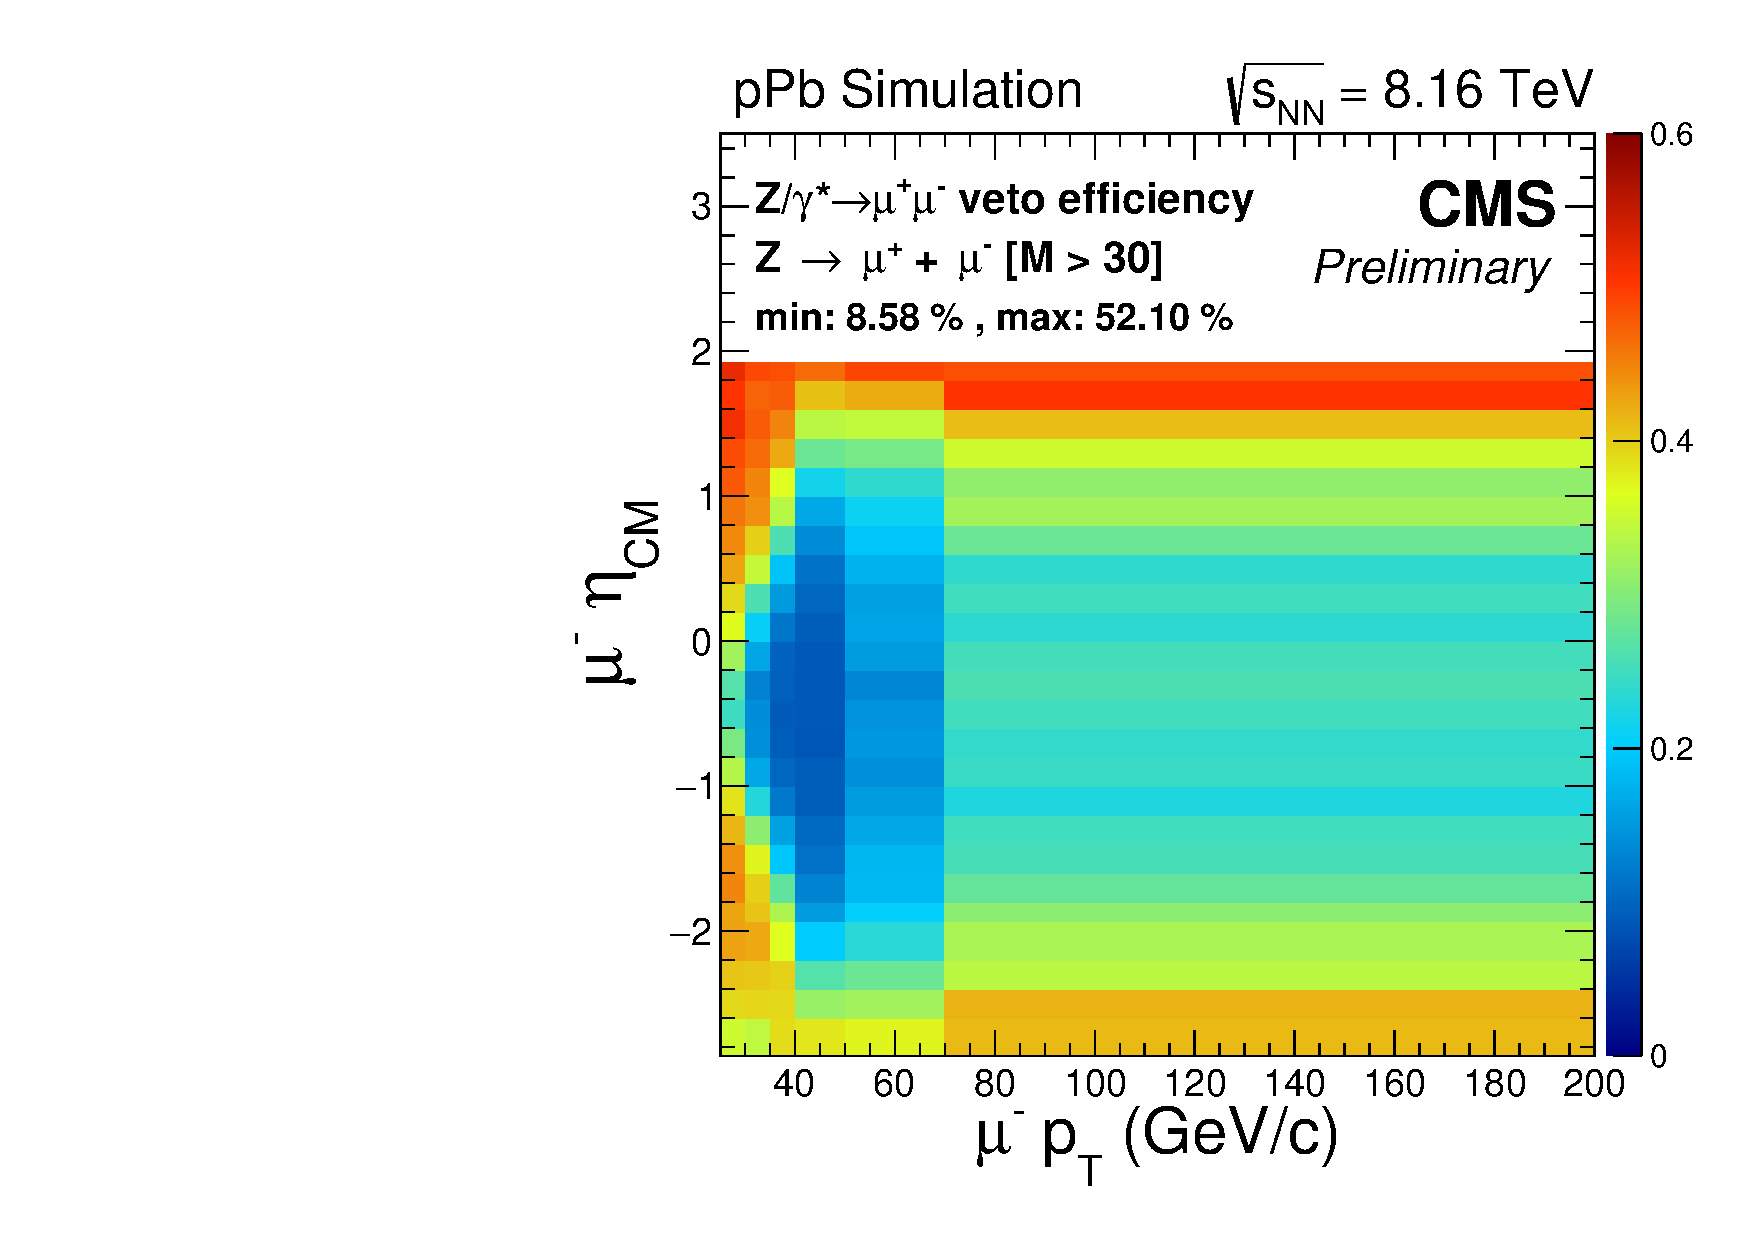
\includegraphics[width=0.45\textwidth]{Figures/WBoson/Analysis/Efficiency/eff2D_Pt_EtaCM_MC_ZToMuMu_M_30_Inf_PA_Minus_DrellYanVeto}
 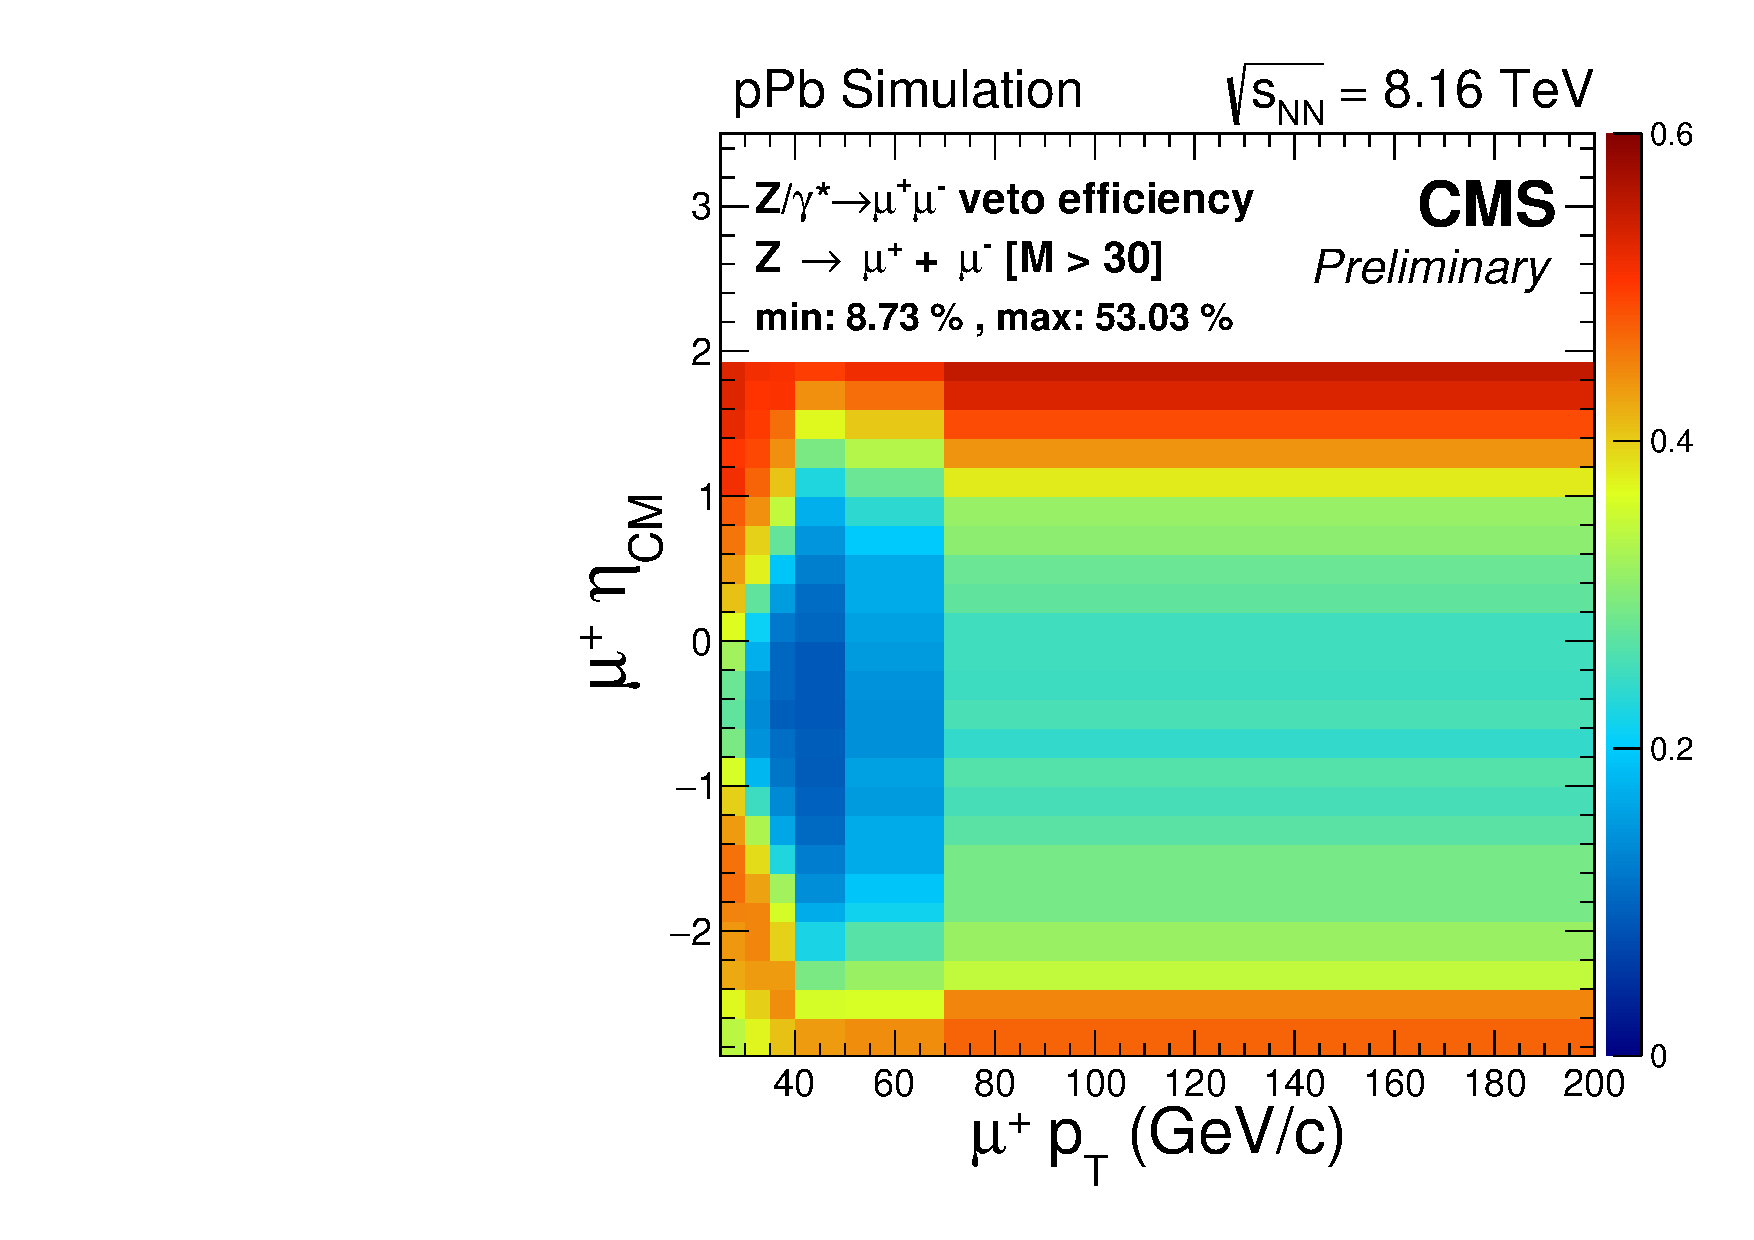
\includegraphics[width=0.45	\textwidth]{Figures/WBoson/Analysis/Efficiency/eff2D_Pt_EtaCM_MC_ZToMuMu_M_30_Inf_PA_Plus_DrellYanVeto}
 \caption{Survival probability of single muons from a \DYToMuMu (M$ > 30$~\GeVcc) simulation, as a function of the muon \etaMuCM and \ptMu, separated in negative (left) and positive (right) charged muons. Muons are required to have $\pt > 25$~\GeVc and $|\eta| < 2.4$, match the trigger and pass the isolation and identification criteria.}
 \label{fig:DrellYanVetoZEfficiency2D}
\end{figure}


%%------------------------------------------------------------%%
\subsubsection{Event selection summary} \label{sec:WBoson_Analysis_Selection_WSelection}

In summary, the signal selection consists of the detection of a high-\pt muon, passing the identification criteria detailed in \sect{sec:WBoson_Analysis_Selection_MuonIdentification}. The muon candidate is required to have $\pt > 25$~\GeVc, be isolated and match the trigger (see \sect{sec:WBoson_Analysis_Selection_Trigger}). The events entering the signal region are also required to satisfy the \RunpPb global event filter (\sect{sec:WBoson_Analysis_Selection_EventFilter}) and the \DYToMuMu veto (\sect{sec:WBoson_Analysis_Selection_DrellYanVeto}).

The other signature of a \WToMuNu event is a high-\pt neutrino, estimated through the \ptmiss. No explicit selection is applied on the missing transverse momentum. The \ptmiss is directly used to extract the event yields by fitting the signal and background components. Apart from the main signal sample, two more samples are used:
\begin{itemize}
 \item \ZToMuMu control sample: selects \ZToMuMu events by reverting the \DYToMuMu veto and selecting \mumu pairs with invariant mass within the \Z-boson mass window. Used to derive corrections for the weak boson \pt (\sect{sec:WBoson_Analysis_Corrections_WeakBosonPTReweighing}) and the \ptmiss (\sect{sec:WBoson_Analysis_Corrections_MET}).
 \item \QCD jet control sample: selects non-isolated muon events by reverting the muon isolation cut. Used to determine the shape of the QCD jet background from data.
\end{itemize}

The conditions used to define the signal and control regions of interest are illustrated in \fig{fig:EventSelectionDiagram}.

\begin{figure}[htb]
 \centering
 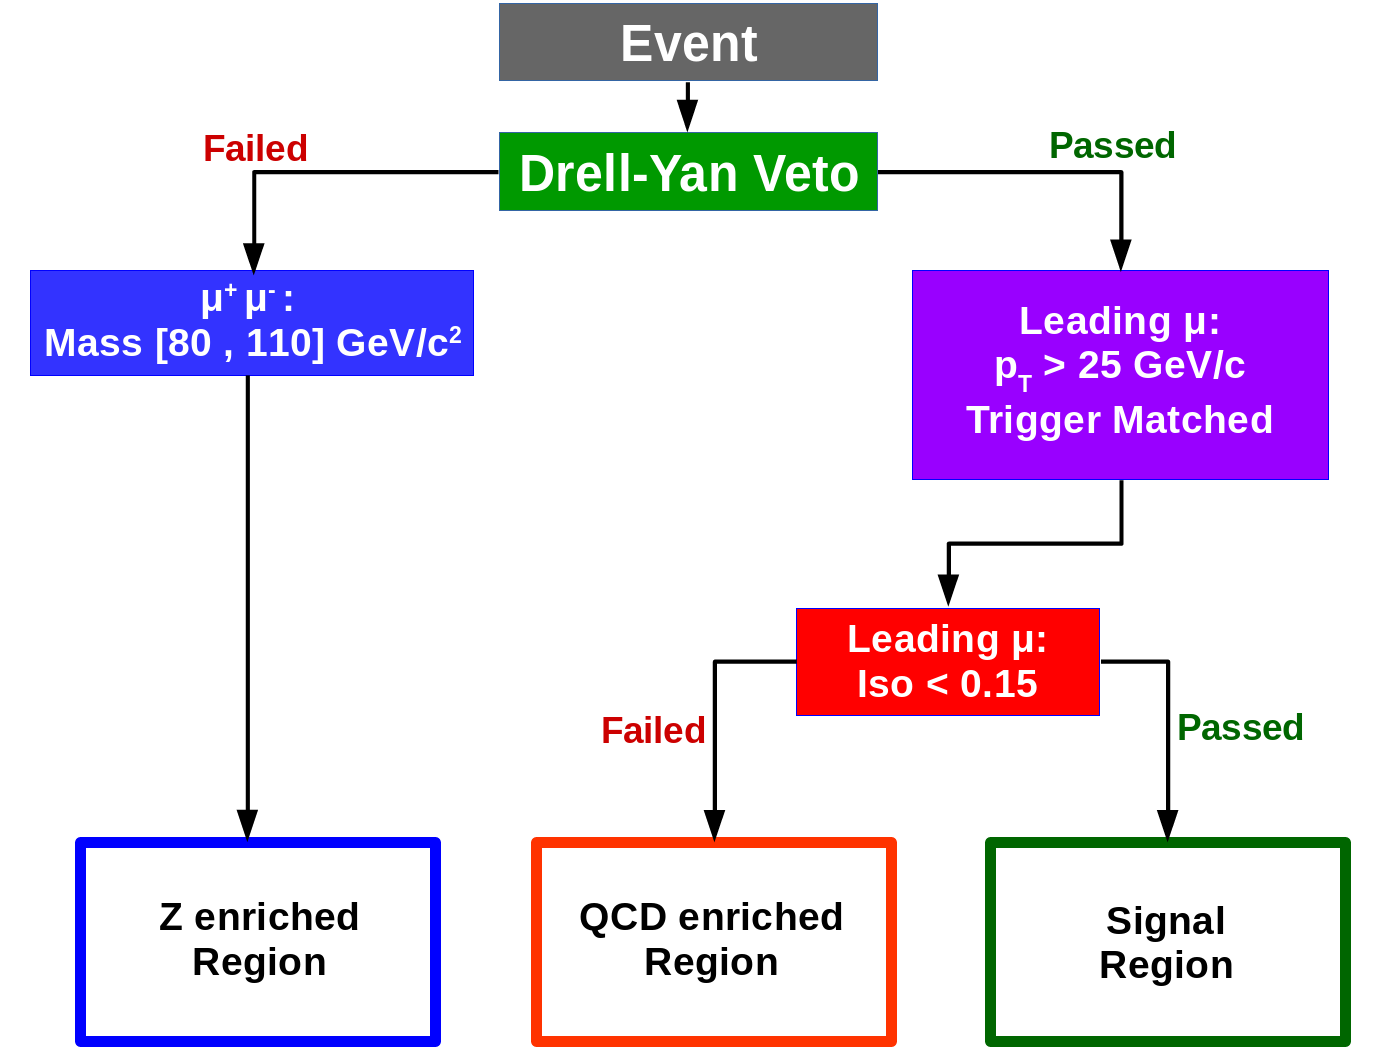
\includegraphics[width=0.8\textwidth]{Figures/WBoson/Analysis/EventSelection/FlowChar.png}
 \caption{Flowchart illustrating the way the events are classified}
 \label{fig:EventSelectionDiagram}
\end{figure}

% END OF SUBSECTION


\subsection{Correction for weak-boson transverse momentum} \label{sec:WBoson_Analysis_Corrections_WeakBosonPTReweighing}

In a \RunpPb collision at high energies, the partons can be described as moving collinearly with the proton or the \Pb nucleus, contributing momentum only along the beam axis. As a result, at leading order, \Wb and \Z bosons are produced with no transverse momentum. Higher order processes, such as NLO or next-to-NLO, can radiate quarks and gluons that recoil against the weak boson, which acquires transverse momentum in the process.

Since the simulations were produced using the \POWHEG NLO generator, the absence of higher order contributions can lead to a mismodelling of the weak boson \pt, which can then affect the \pt distribution of the boson decay products (e.g. muon and neutrino). To check this, one can select \ZToMuMu events and compare the \pt distribution of \Z boson candidates from simulation and data.

The \pt distribution of \Z bosons has been measured in an on-going CMS analysis of the Drell--Yan production in \pPb collisions at \SI{8.16}{\TeV}~\footnote{The details of the CMS Drell--Yan analysis can be checked in the private link \url{http://cms.cern.ch/iCMS/analysisadmin/cadilines?line=HIN-18-003&tp=an&id=2036&ancode=HIN-18-003}}, which makes use of the same data and electroweak NLO simulations presented in this chapter. As part of the DY analysis, the measurement of the \Z-boson \pt distribution in the dimuon mass region [60 , 120]~\GeVcc was compared, after correcting for acceptance and efficiency, to the generated one from \POWHEG and found to disagree by up to 20\%. To correct for the disagreement, the ratio between the  measured and simulated \pt-differential \ZToMuMu cross sections was parametrised as a function of the \Z-boson \pt, resulting in:

\begin{equation}
 w^{\Z}\left(\pt\right) = \frac{\left(\frac{\dd\sigma[\ZToMuMu]}{\dd\pt}\right)^{\text{data}}}{\left(\frac{\dd\sigma[\ZToMuMu]}{\dd\pt}\right)^{\text{MC}}} = \frac{1}{1.19 -0.37\times\pt^{-0.37}}
 \label{eq:DY_DatavsMC}
\end{equation}

and the generated \Z-boson \pt distribution was then weighed per event using $w^{\Z}\left(\pt\right)$.

Considering that \Z and \Wb bosons have similar production mechanisms and masses, $w^{\Z}\left(\pt\right)$ is also used to weigh, on an event-by-event basis, the generated \Wb-boson \pt spectrum. The boson \pt weighing is applied to the \POWHEG simulations of both signal (\WToMuNu) and electroweak backgrounds (\WToTauNu , \DYToMuMu and \DYToTauTau).

The impact of the boson \pt weighing is checked on a \Wb-boson enhanced sample in data and simulation, made by applying a requirement on the transverse mass, defined as $M_{\text{T}} = \sqrt{\pt^{\mu}\cdot\ptmiss\cdot(1-\cos\left({\Delta{\theta}}\right))}$, where $\Delta{\theta}$ is the azimuthal angle between the \ptvecmiss and muon $\ptvec^{\mu}$. The events of the \Wb-boson enhanced sample are selected from the signal region by requiring $M_{\text{T}} > 60$~\GeVc, and the corresponding muon \pt distribution is then compared before and after applying the boson \pt weighing in \fig{fig:WEventPTDist}. The simulated muon \pt distribution is observed to describe better the data  in the high-\pt region ($\pt^{\mu} \gtrsim 40$~\GeVc) after weighing the generated \Wb-boson boson \pt distribution.

\begin{figure}[htb!]
 \centering
  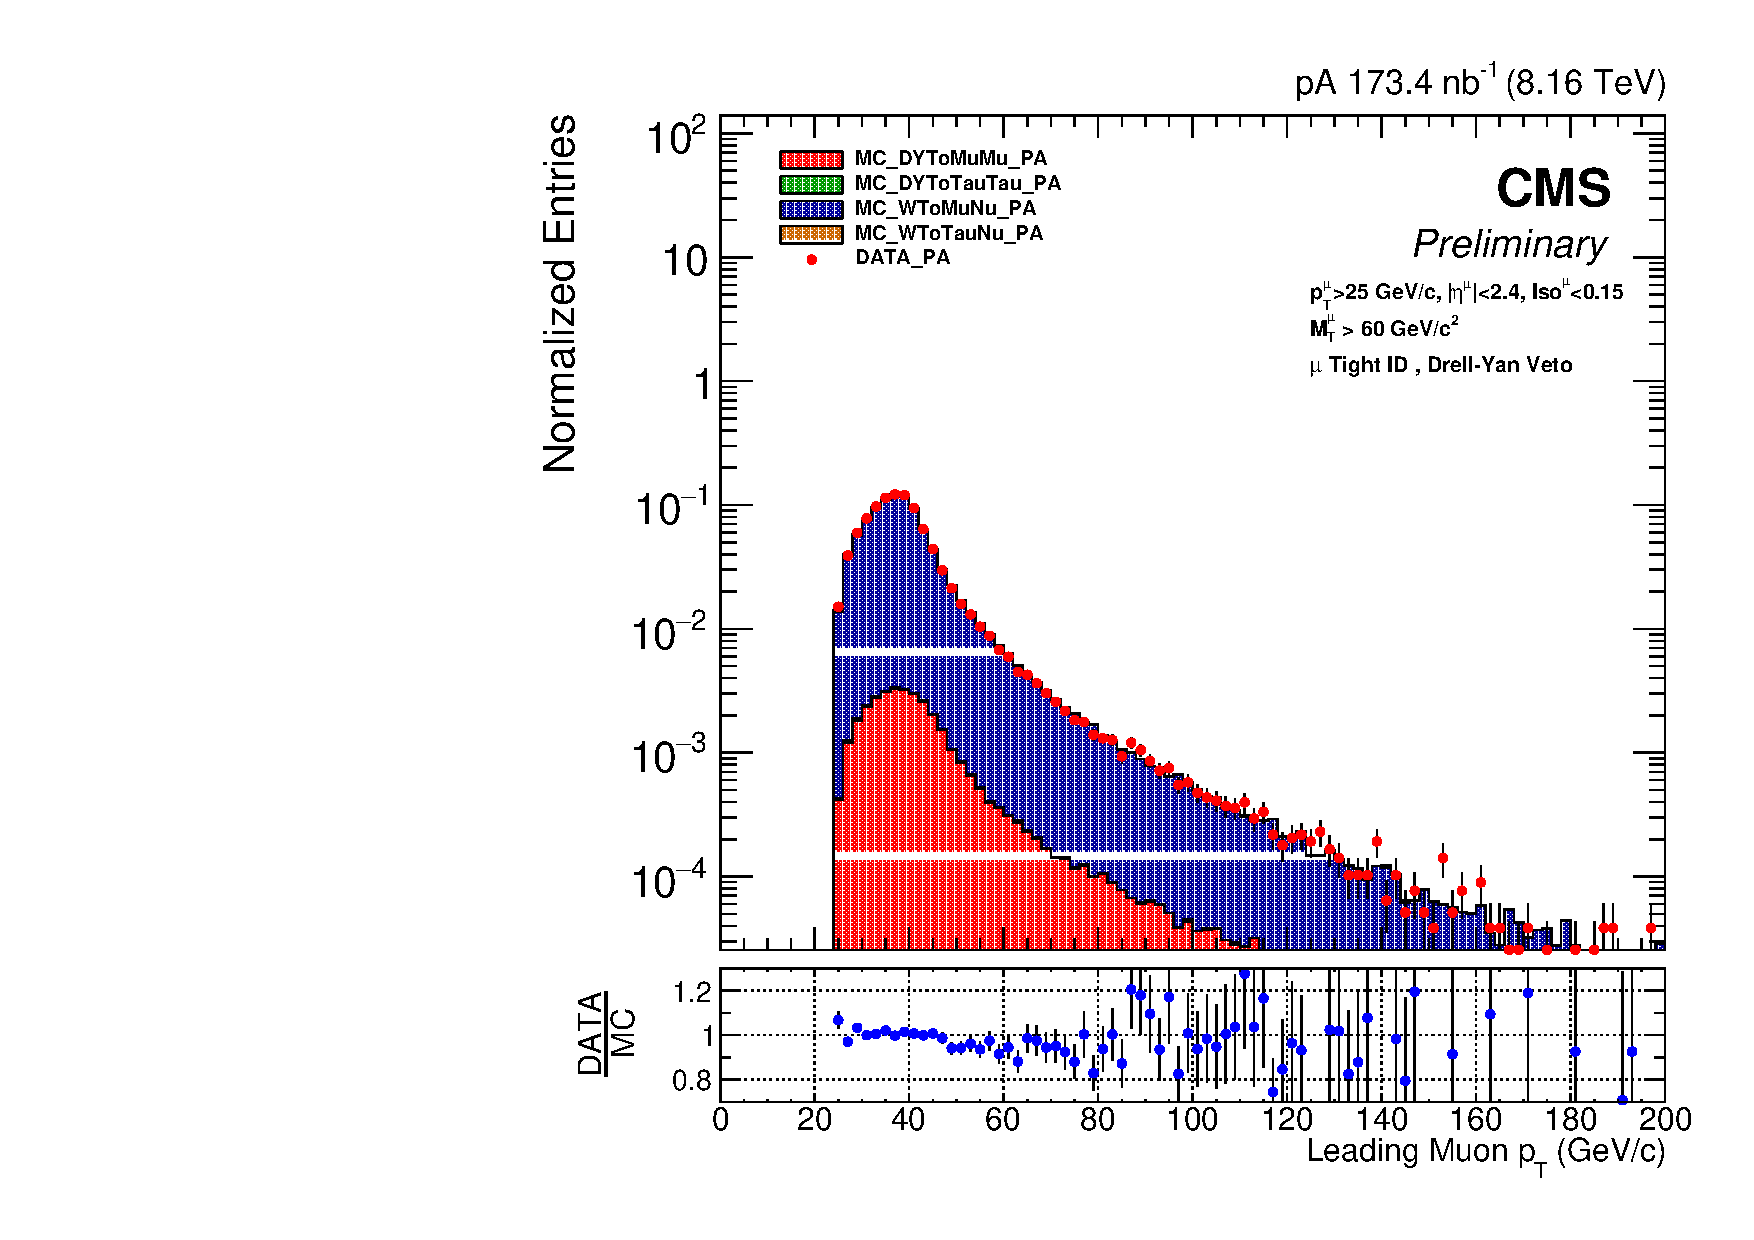
\includegraphics[width=0.45\textwidth]{Figures/WBoson/Analysis/Correction/BosonPT/c_DATAvsMCStack_MC_PA_WToMu_Plus_Mu_PT.pdf}
  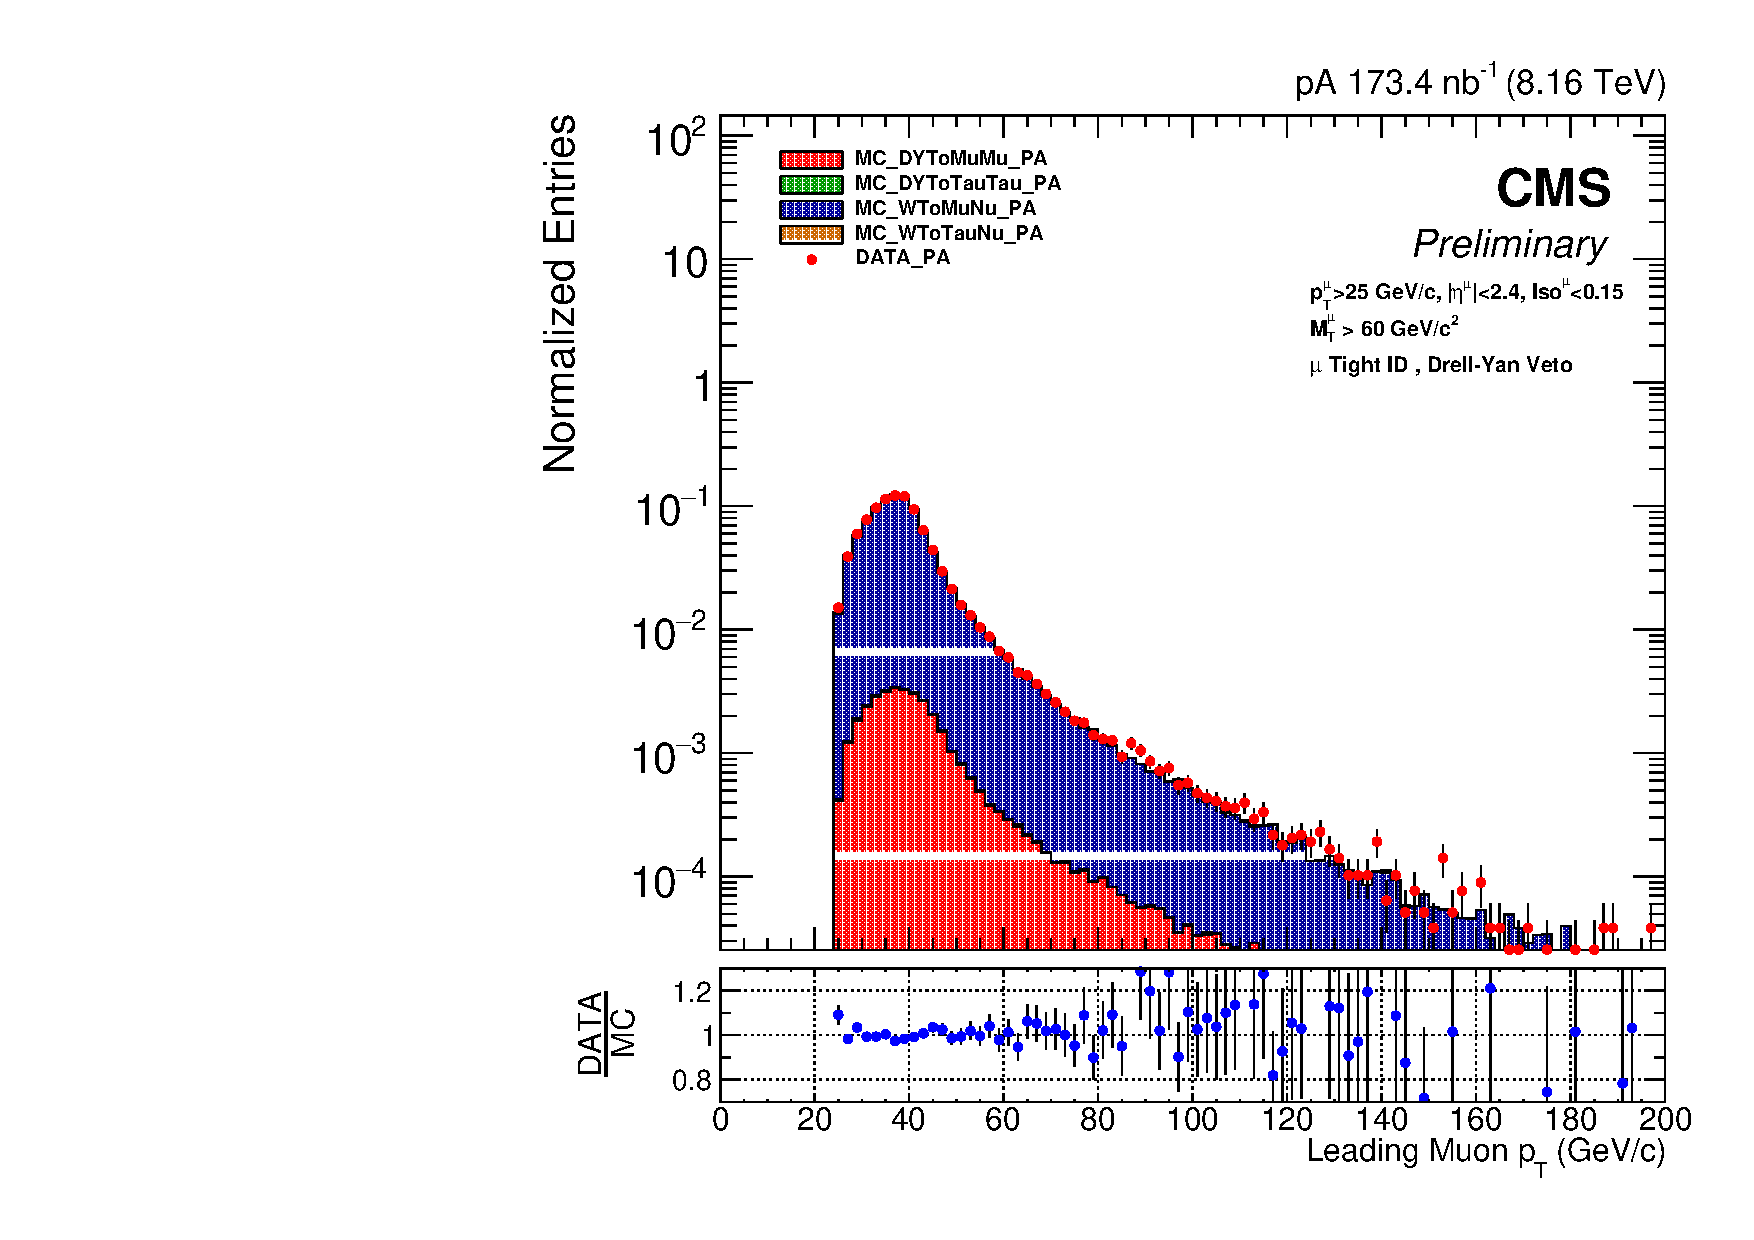
\includegraphics[width=0.45\textwidth]{Figures/WBoson/Analysis/Correction/BosonPT/c_DATAvsMCStack_MC_PA_WToMu_Plus_Mu_PT_NOMINAL.pdf}
 \caption{Muon \pt distribution extracted from the \Wb-boson enhanced sample before (left) and after (right) applying the boson \pt weights. The red points correspond to data, while the blue and red filled areas correspond to events from the \WToMuNu and \DYToMuMu simulations, respectively. The bottom panels shows the ratio of data over simulation.}
 \label{fig:WEventPTDist}
\end{figure}


\subsection{Corrections for missing transverse momentum} \label{sec:WBoson_Analysis_Corrections_MET}

Since the \Wb-boson analysis relays on \ptmiss distributions from simulations to extract the signal, it is important that the simulated \ptmiss describes the data. To achieve this, the \pt distribution of the reconstructed particles, including those recoiling against the weak boson (referred as the recoil), have to be well modelled.

The \ptmiss vector derived from \WToMuNu events can be decomposed, according to \eq{eq:MET}, in two parts: the \pt vector of the muon candidate (\ptMuvec) and the \pt vector of the recoil (\utvec), as defined in:

\begin{equation}
 \ptvecmiss = -\left( \utvec + \ptMuvec \right )
 \label{eq:METSep}
\end{equation}

The recoil \utvec is measured via the \ptvec vectorial sum of all particles identified in an event with the PF algorithm \textit{excluding} the muon from the \Wb-boson decay, as given by:

\begin{equation}
 \utvec = \left(\sum_{\text{particles}} \ptvec\right) - \ptMuvec
 \label{eq:recoil}
\end{equation}

The recoil is a complex quantity that includes particles from the hard scattering that balances the \Wb-boson \pt and from the underlying event (e.g. spectator parton interactions and multiple parton scatterings), as well as effects related to the detector (e.g. electronic noise, \pt resolution, reconstruction efficiency and acceptance) and the accelerator (e.g. beam-beam remnants). As a result, the recoil is difficult to simulate precisely in \RunpPb collisions and the mismodelling of the recoil \ut can affect the signal extraction.

To improve the modelling of the \ptmiss in the signal region, the \ptmiss is corrected in two steps. First, the distribution of the simulated event activity measured as a function of the total energy deposited in the HF calorimeter (hereafter referred as the HF energy) is weighed to the level observed in data as detailed in \sect{sec:WBoson_Analysis_Corrections_EventActivityReweighing}. Afterwards, the simulated recoil is calibrated following the procedure described in \sect{sec:WBoson_Analysis_Corrections_RecoilCalib}.

\subsubsection{Event activity weighing}\label{sec:WBoson_Analysis_Corrections_EventActivityReweighing}

The muon isolation and the \ptmiss are computed by summing over particles produced in the event. As a consequence, any disagreement in the modelling of the event activity (EA) can impact the muon efficiency and the signal extraction. The disagreement between data and the \POWHEG simulations embedded in \EPOS minimum bias events can be caused by the presence of hard probes such as \Wb bosons, which bias the event activity towards higher particle  multiplicity compared to minimum bias events.

To check if the event activity is well modelled in the simulations, the distribution of the number of tracks per event and the HF energy is compared between data and simulation in a \ZToMuMu control sample. The \ZToMuMu events are selected by requiring a \mumu pair within the invariant mass region $80 < M_{\mumu} < 110$~\GeVcc as detailed in \sect{sec:WBoson_Analysis_Selection_WSelection}. The data-simulation comparisons are shown in \fig{fig:HFNoCorr}, and it is observed that the simulated samples are indeed not able to reproduce the event activity present in \RunpPb data.

\begin{figure}[htb!]
 \centering
  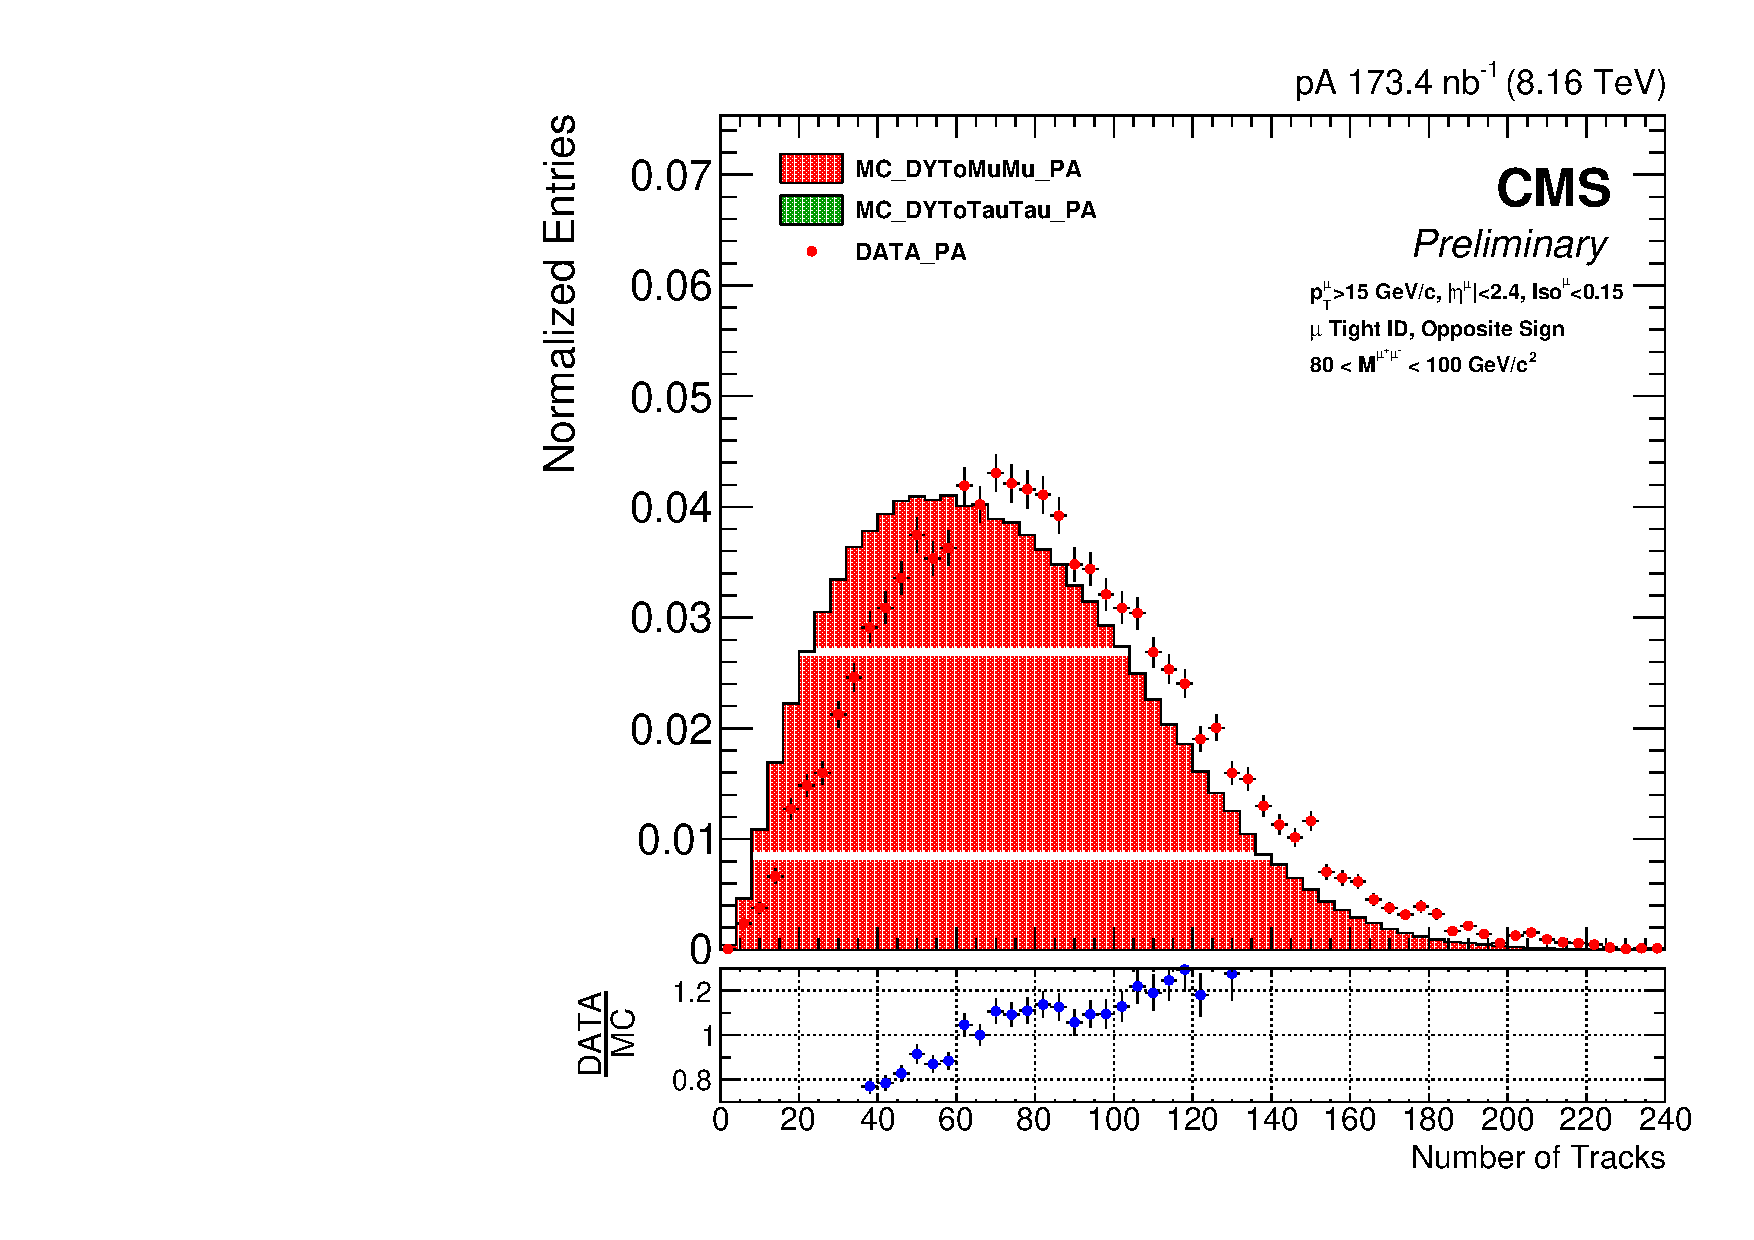
\includegraphics[width=0.40\textwidth]{Figures/WBoson/Analysis/Correction/EventActivityReweighing/c_DATAvsMCStack_MC_PA_ZToMuMu_Track_N.pdf}
  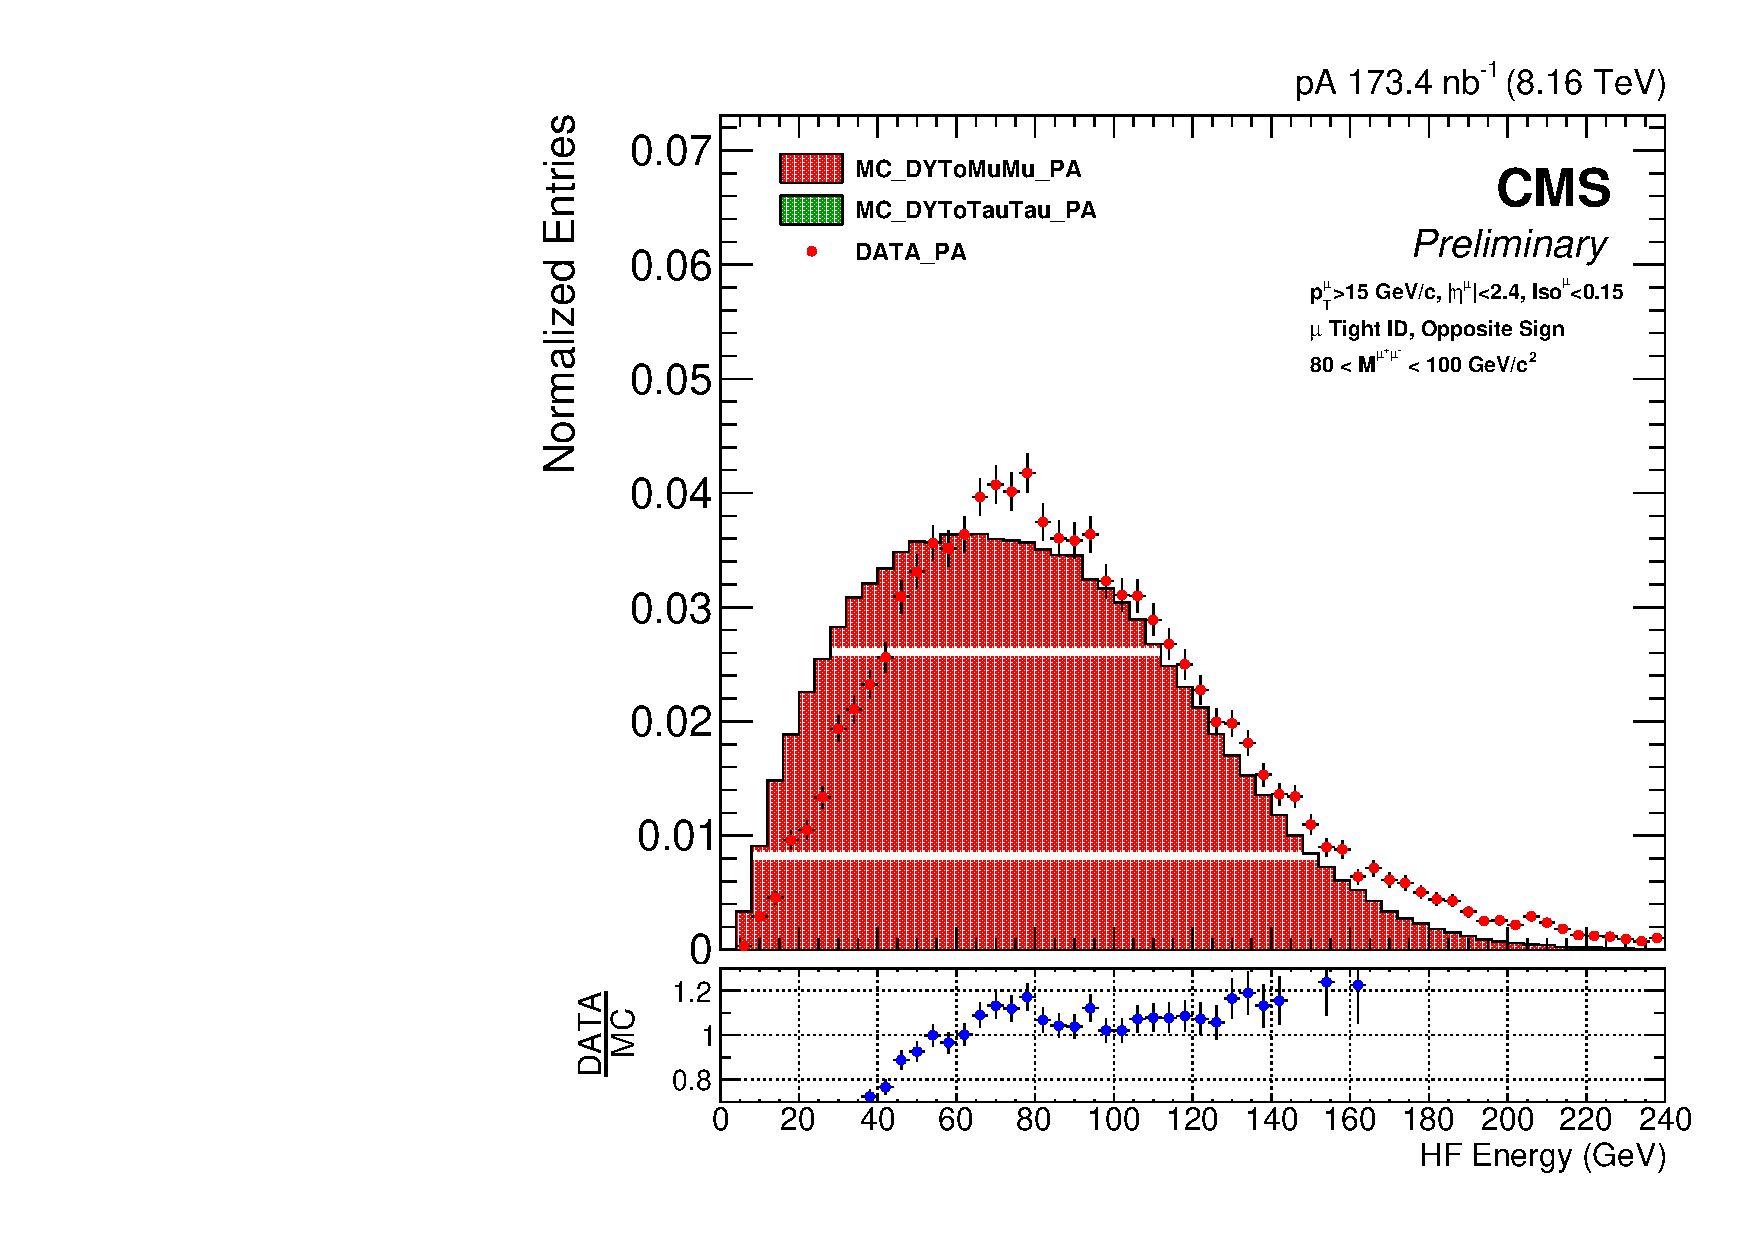
\includegraphics[width=0.40\textwidth]{Figures/WBoson/Analysis/Correction/EventActivityReweighing/c_DATAvsMCStack_MC_PA_ZToMuMu_HF_E.pdf}
 \caption{Distribution of the number of tracks per event (left) and the total energy deposited in the HF calorimeter (right) in \ZToMuMu events. The red points and filled area correspond to data and \DYToMuMu simulation, respectively.}
 \label{fig:HFNoCorr}
\end{figure}

The modelling of the event activity is improved using a set of weights determined from the ratio of the number of \ZToMuMu events extracted from data and simulation in different bins of HF energy ($E_{\text{HF}}$), as given by:

\begin{equation}
 w^{\text{EA}}\left(E_{\text{HF}}\right) = \frac{N_{\ZToMuMu}^{\text{data}}\left[E_{\text{HF}}\right]}{N_{\ZToMuMu}^{\text{MC}}\left[E_{\text{HF}}\right]}
\end{equation}

The $w^{\text{EA}}\left(E_{\text{HF}}\right)$ weights are used, event-by-event, to weigh the HF energy distribution of the electroweak and \ttbar simulations. \fig{fig:HFrewCheck} shows that the HF energy weighing improves the simulation-to-data agreement of the \ptmiss distribution of \ZToMuMu events. The remaining level of disagreement in the \ptmiss is then corrected for by calibrating the simulated recoil as explained in the next section.

\begin{figure}[htb!]
 \centering
 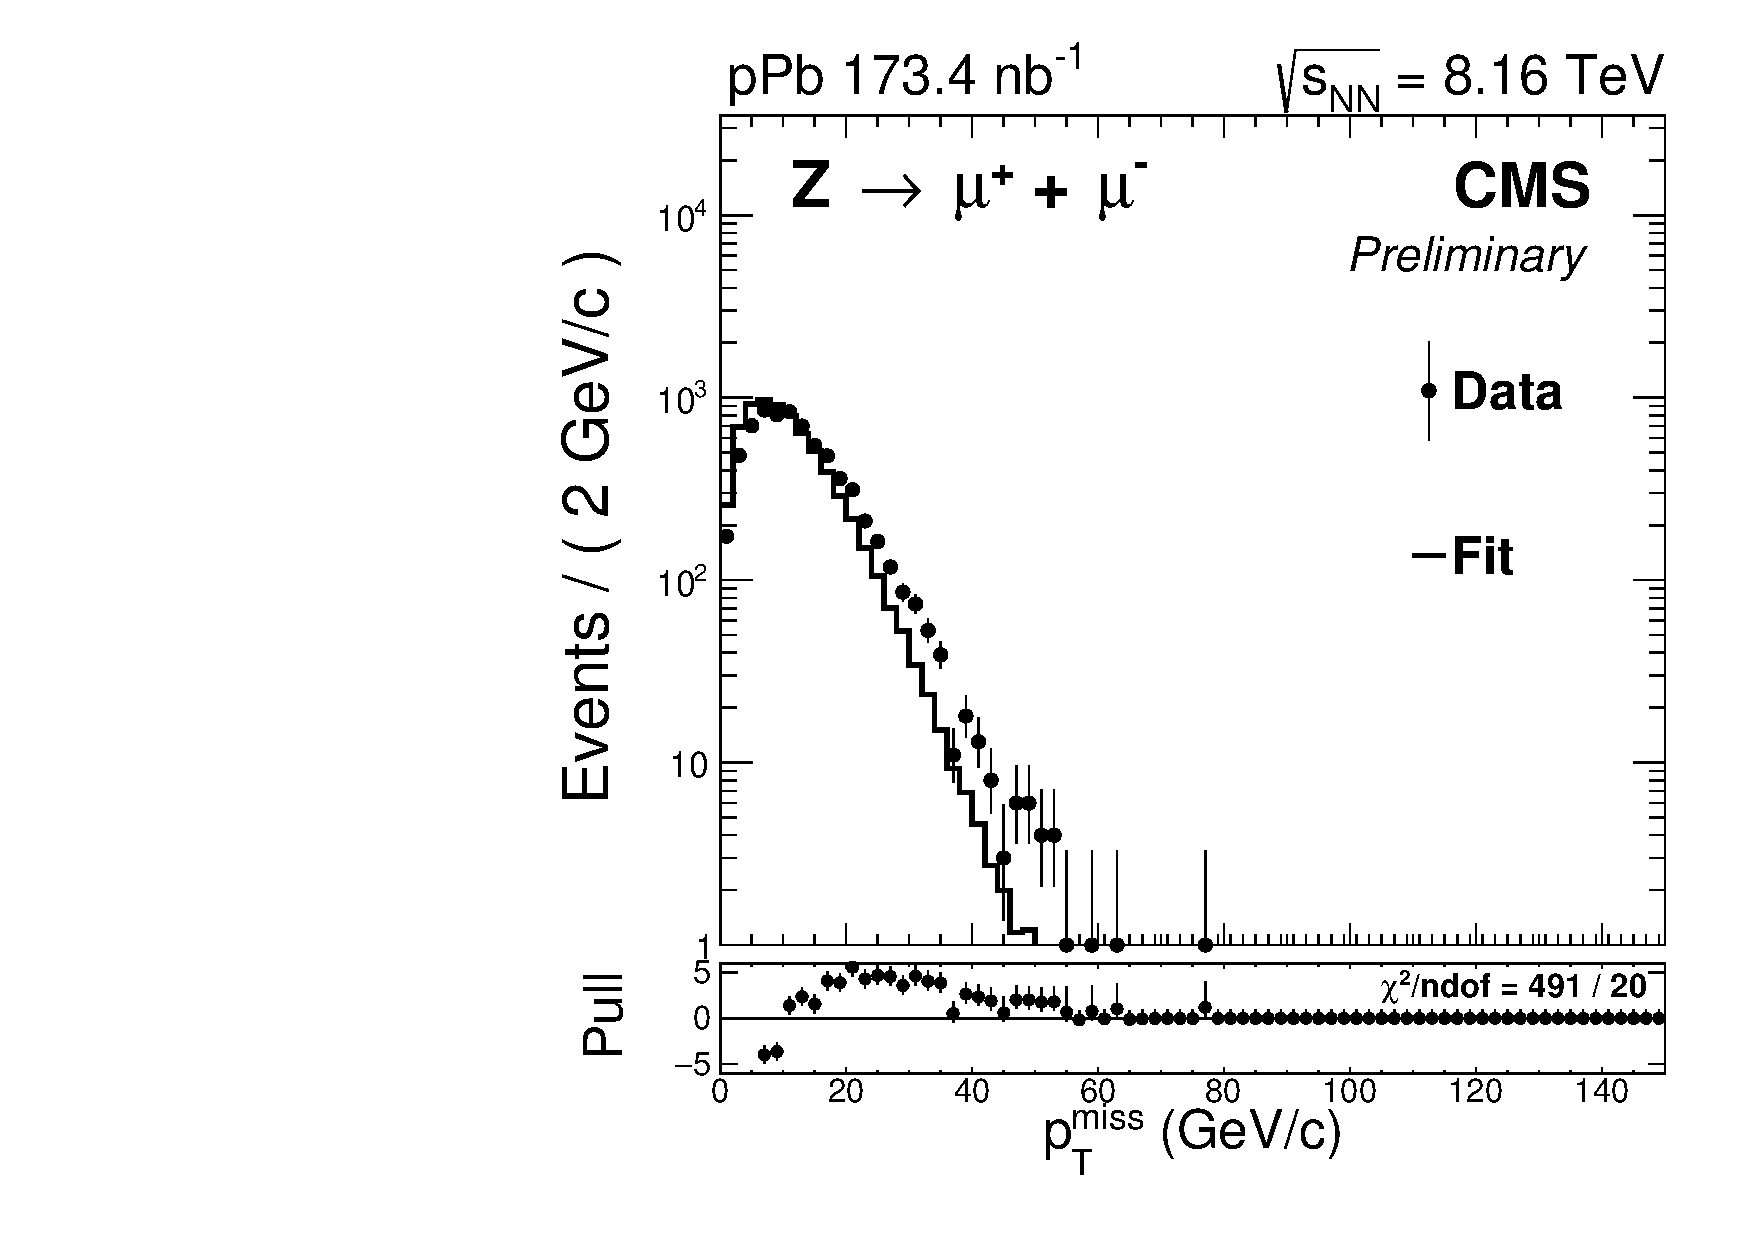
\includegraphics[width=0.4\textwidth]{Figures/WBoson/Analysis/Correction/Recoil/CheckFits/Z/METPF_RAW/PLOT_MET_DATA_ZToMuPl_PA_Model_TEMP_DY_MuEtaCM_-286_193_MuIso_0_15.pdf}
 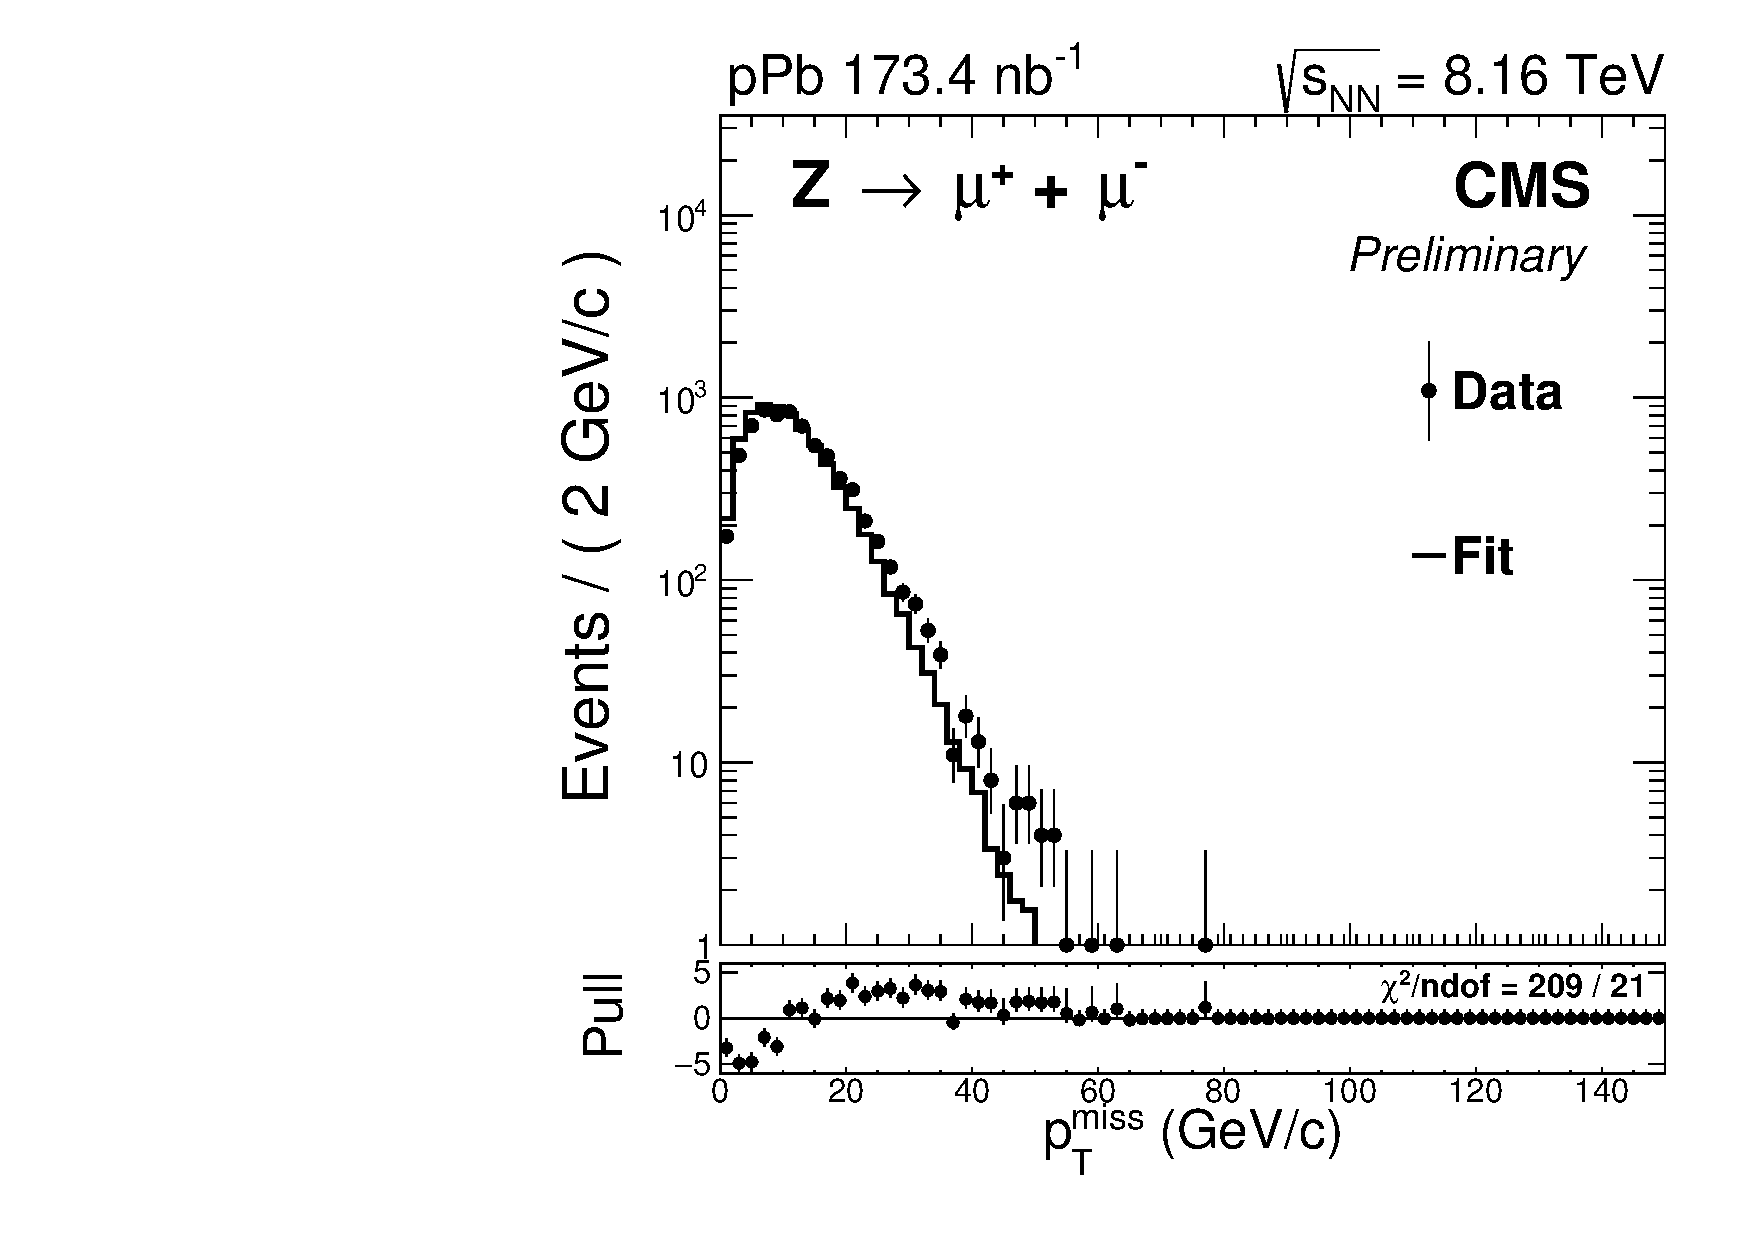
\includegraphics[width=0.4\textwidth]{Figures/WBoson/Analysis/Correction/Recoil/CheckFits/Z/METPF_RAW_HFrew/PLOT_MET_DATA_ZToMuPl_PA_Model_TEMP_DY_MuEtaCM_-286_193_MuIso_0_15.pdf}
 \caption{Comparison of the \ptmiss distribution in data and simulation for \ZToMuMu events before (left) and after (right) applying the HF energy weights.}
 \label{fig:HFrewCheck}
\end{figure}


\subsubsection{Recoil calibration} \label{sec:WBoson_Analysis_Corrections_RecoilCalib}

The recoil calibration procedure starts by measuring the recoil in \ZToMuMu events in data and simulation, and then parametrise, in each sample, the components of the recoil \utvec with respect to the transverse momentum of the \Z boson (\qtZ). Afterwards, these parametrisations are used to scale in each event the simulated \utvec components according to the weak boson \pt, from each electroweak simulation, to match the average recoil distribution measured in data.

The \ZToMuMu control sample employed to extract the recoil calibration is the same as the one used to derive  the event activity weights described in the previous section. In addition, the simulated HF energy and the generated \Z-boson \pt distributions of the control sample have been weighed accordingly.

\paragraph{Extraction of the recoil scale and resolution.} Since there are no neutrinos produced in the initial hard scattering of \ZToMuMu events, the \ptmiss spectrum can be used to directly measure the \ptmiss resolution. \fig{fig:METZBoson} compares the \ptmiss spectra extracted from data and simulation in the \ZToMuMu control sample. It is observed that the simulation does not properly describe the \ptmiss distribution measured in data.

\begin{figure}[htb!]
 \centering
 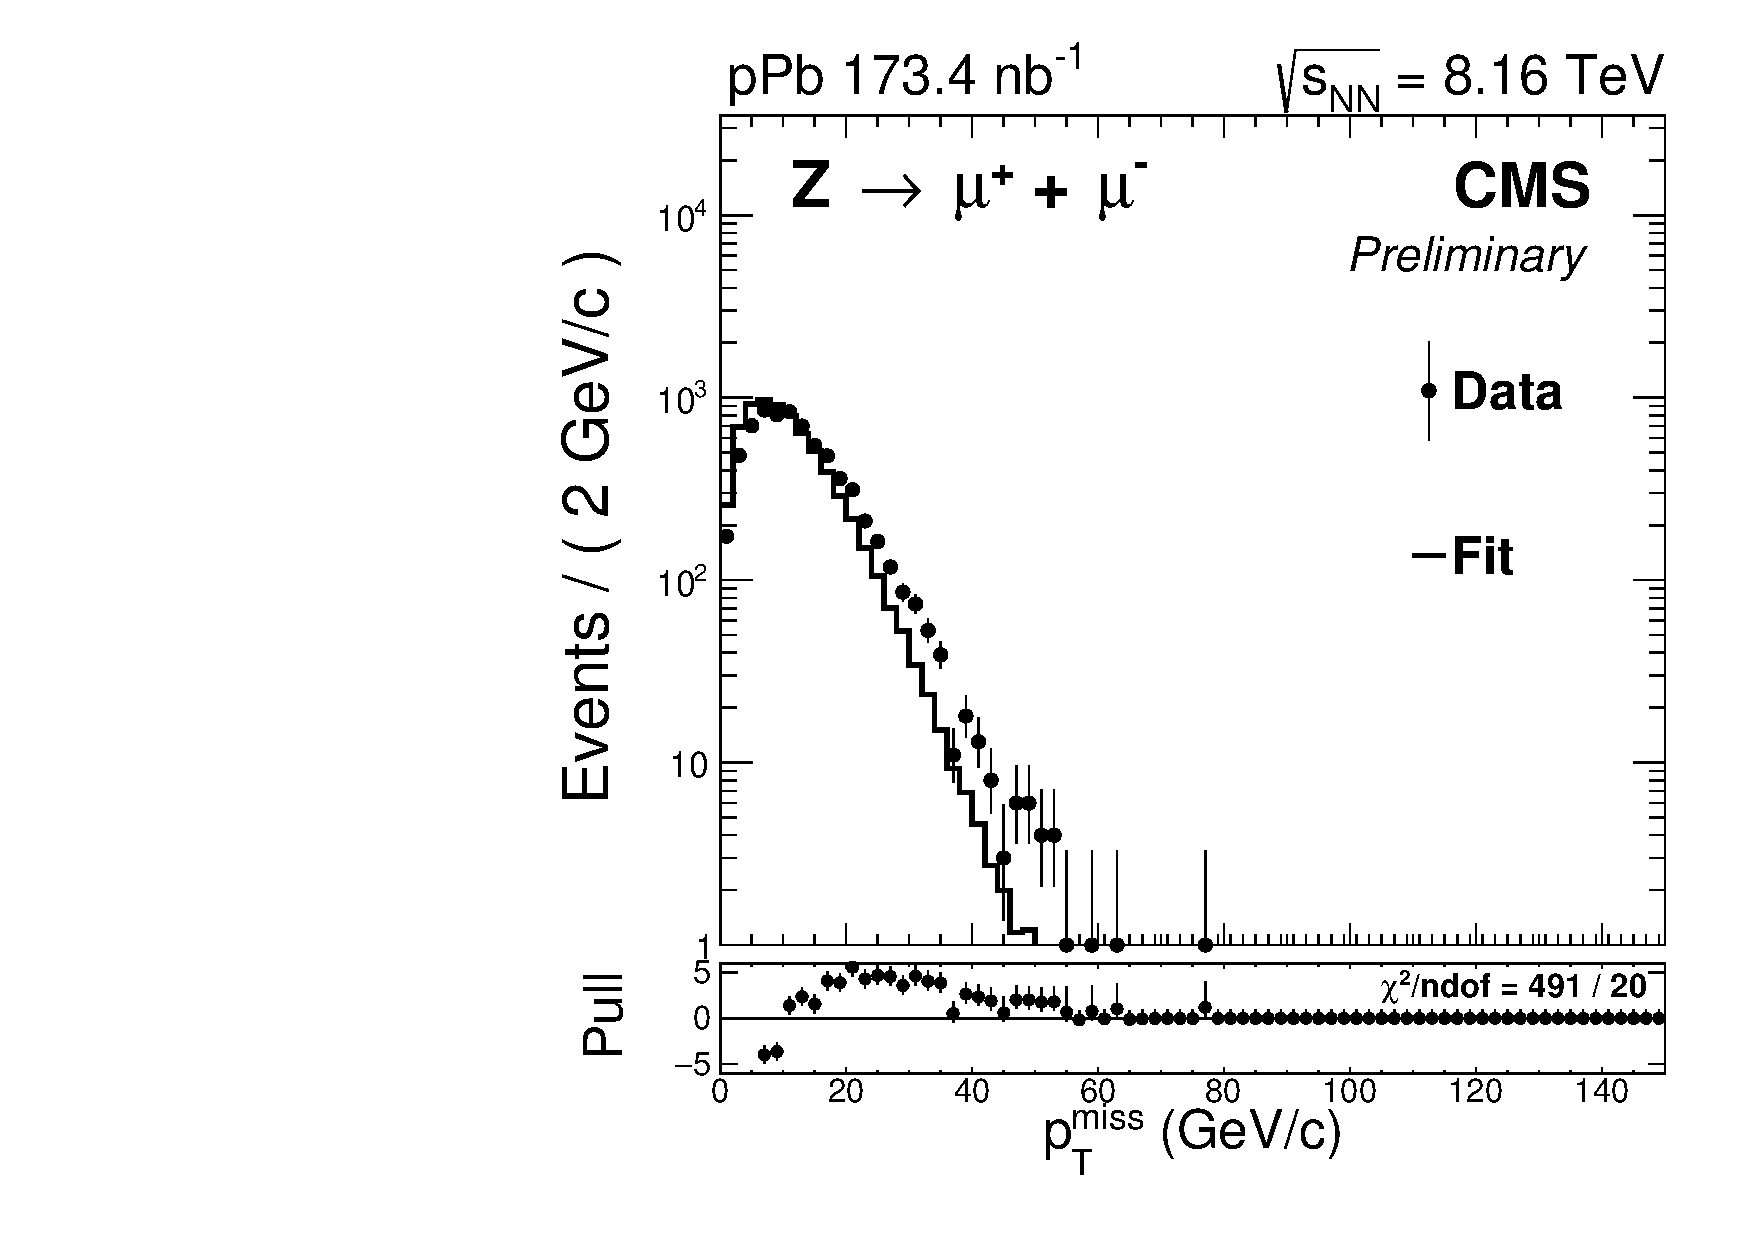
\includegraphics[width=0.5\textwidth]{Figures/WBoson/Analysis/Correction/Recoil/CheckFits/Z/METPF_RAW/PLOT_MET_DATA_ZToMuPl_PA_Model_TEMP_DY_MuEtaCM_-286_193_MuIso_0_15.pdf}
 \caption{Distribution of the \ptmiss in data and simulation for \ZToMuMu selected events.}
 \label{fig:METZBoson}
\end{figure}

In the case of \ZToMuMu events, the recoil \utvec is measured by \textit{subtracting} the \pt vector of the \Z-boson candidate ($\qtZvec = \ptvec^{\mu^{+}} + \ptvec^{\mu^{-}}$) from the \ptvecmiss, according to:

\begin{equation}
 \utvec = -\ptvecmiss - \qtZvec
 \label{eq:recoilZBoson}
\end{equation}

The recoil \utvec is then projected along the \Z-boson \qtZvec direction. The parallel and perpendicular components of \utvec, with respect to the \qtZvec, are labelled as \utpar and \utper, respectively. \fig{fig:RecoilComp} shows the components of the recoil in \ZToMuMu events.

\begin{figure}[htb!]
 \centering
 \begin{tikzpicture}
  \draw[dashed, thick] (-4.4,0)--(4.4,0) node[right]{};
  \draw[dashed, thick] (0,-3.0)--(0,3.0) node[above]{};
  \draw[line width=2pt,black,-stealth](0,0)--(-2.8,-1.2) node[anchor=north west]{\utvec};
  \draw[line width=1pt,black,-stealth](-2.8,0)--(-2.8,-1.2) node[anchor=south east]{\utpar};
  \draw[line width=1pt,black,-stealth](0,0)--(-2.8,0) node[anchor=south west]{\utper};
  \draw[dashed,->,black,thick](0,0)--(-1.2,1.2) node[anchor=south east]{\ptvecmiss};
  \draw[line width=1pt,black,-stealth](0,0)--(2,-2) node[anchor=south west]{$\ptvec\left(\mu^{+}\right)$};
  \draw[line width=1pt,black,-stealth](0,0)--(2,2) node[anchor=south west]{$\ptvec\left(\mu^{-}\right)$};
  \draw[line width=3pt,black,-stealth](0,0)--(4,0) node[anchor=south west]{$\qtvec\left(\text{Z}\right)	$};
 \end{tikzpicture}
 \caption{Definition and components of the recoil \utvec for \ZToMuMu events.}
 \label{fig:RecoilComp}
\end{figure}

The \utpar and \utper recoil components are evaluated event-by-event and sorted in 30 bins of \qtZ defined within the range $0 < \qtZ < 140$~\GeVc. The distributions of \utpar and \utper from data and simulation are fitted separately in each \qtZ bin with a weighed sum of two Gaussian functions, according to:

\begin{equation}
 \begin{aligned}
  F\left(u_{\parallel}\right) &= N_{\parallel} \cdot \left( f_{\parallel} \cdot  \exp\left[{\frac{\left(u_{\parallel} - \mu_{\parallel}\right)^{2}}{2 \cdot \sigma_{\parallel,1}^{2}}}\right]  + \left(1-f_{\parallel}\right)\cdot \exp\left[{\frac{\left(u_{\parallel} - \mu_{\parallel}\right)^{2}}{2 \cdot \sigma_{\parallel,2}^{2}}}\right]  \right) \\
  F\left(u_{\perp}\right) &= N_{\perp} \cdot \left( f_{\perp} \cdot  \exp\left[{\frac{\left(u_{\perp} - \mu_{\perp}\right)^{2}}{2 \cdot \sigma_{\perp,1}^{2}}}\right]  + \left(1-f_{\perp}\right)\cdot \exp\left[{\frac{\left(u_{\perp} - \mu_{\perp}\right)^{2}}{2 \cdot \sigma_{\perp,2}^{2}}}\right]  \right)
 \end{aligned}
 \label{eq:gaussFit}
\end{equation}

where $N_{\parallel(\perp)}$ corresponds to the number of events in each \qtZ bin, $f_{\parallel(\perp)}$ is the weight of the Gaussian components, $\mu_{\parallel(\perp)}$ is the mean of the Gaussian functions, and $\sigma_{\parallel(\perp),1}$ and $\sigma_{\parallel(\perp),2}$ are the corresponding Gaussian widths. The parameters $f_{\parallel}$ and $f_{\perp}$ are fixed to: $f_{\parallel} = f_{\perp} = 0.70$ in data and $f_{\parallel} = f_{\perp} = 0.45$ in simulation, to obtain a better convergence of the fits. The other parameters are left free.

Examples of the distributions of the parallel and perpendicular recoil components are shown in \fig{fig:RecoilFits} for data and simulation. Also, the fits performed with the weighed combination of Gaussian functions and their pull distributions are presented.

\begin{figure}[htb!]
 \centering
 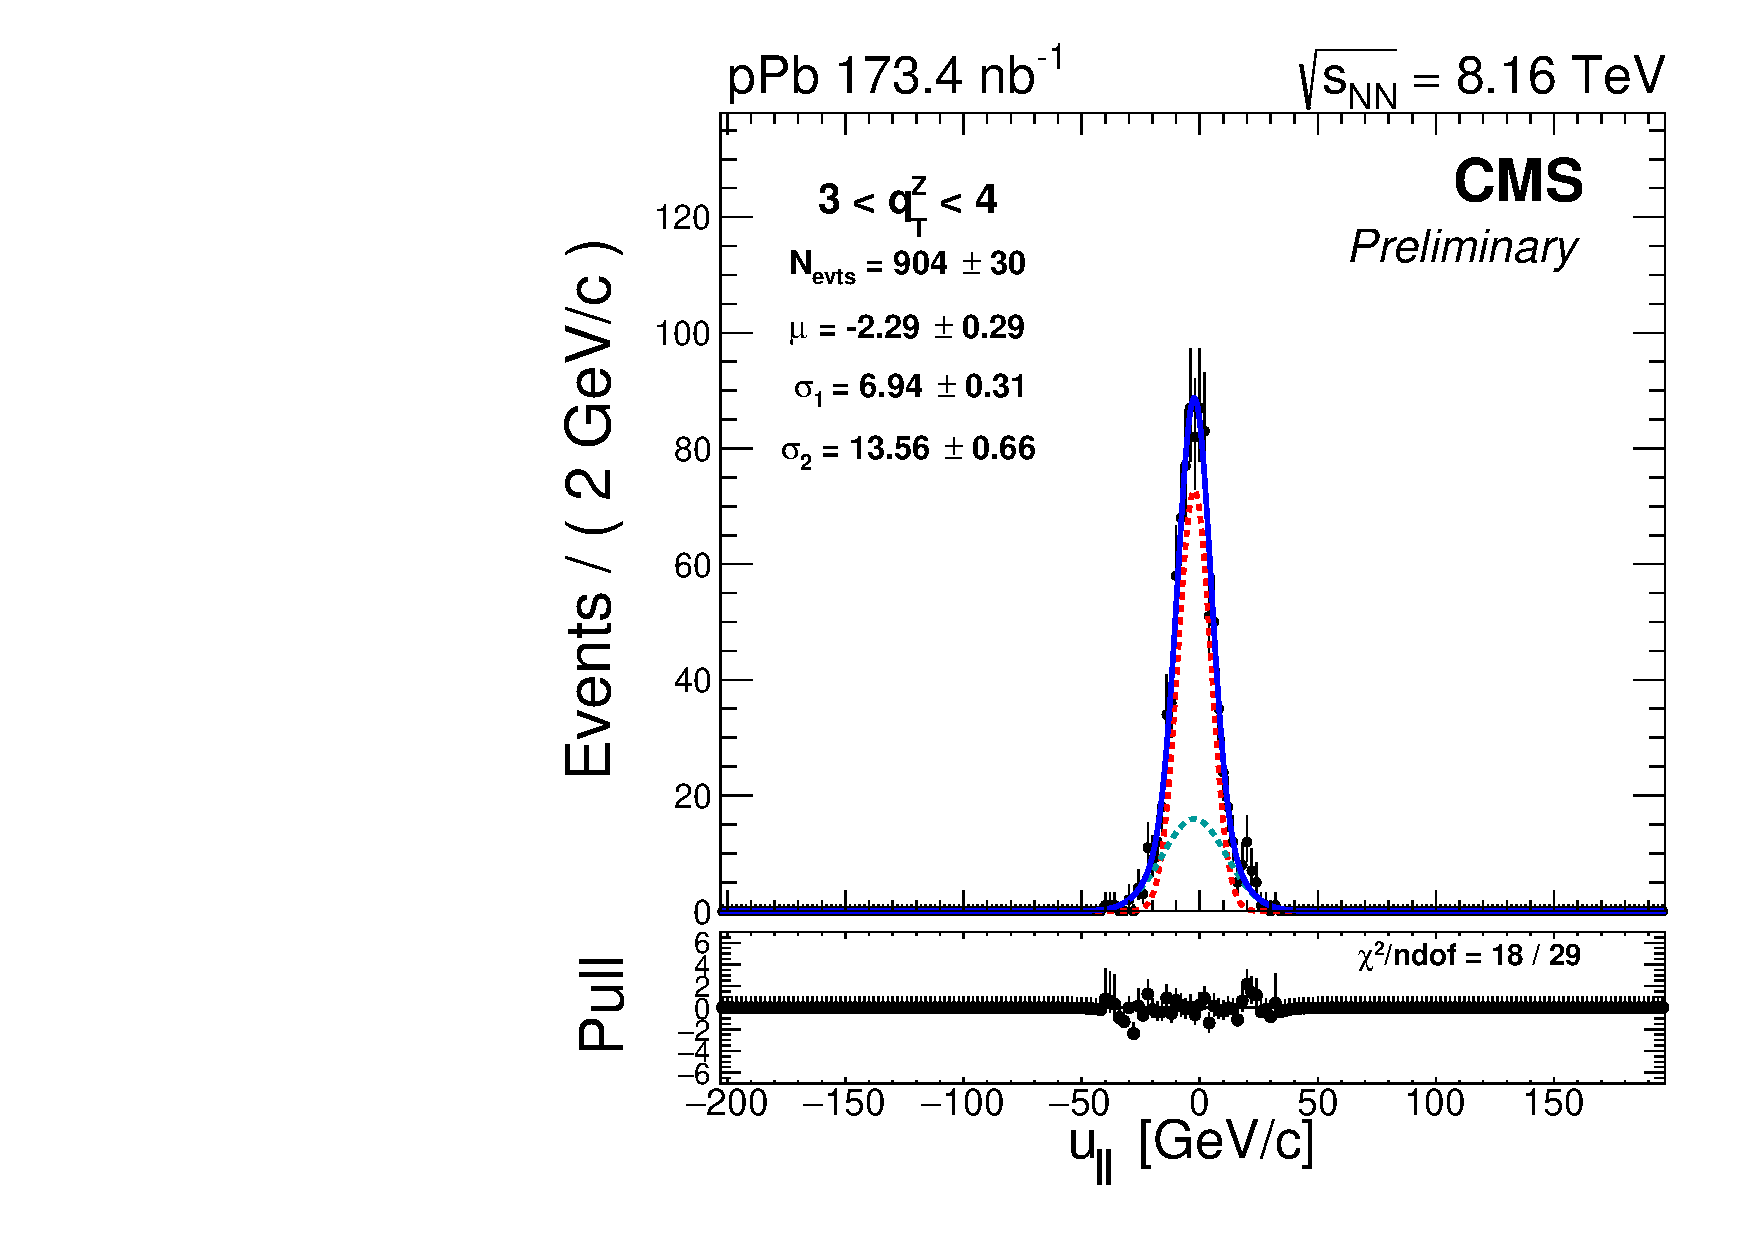
\includegraphics[width=0.4\textwidth]{Figures/WBoson/Analysis/Correction/Recoil/RecoilFits/Data/pfu1fit_2.pdf}
 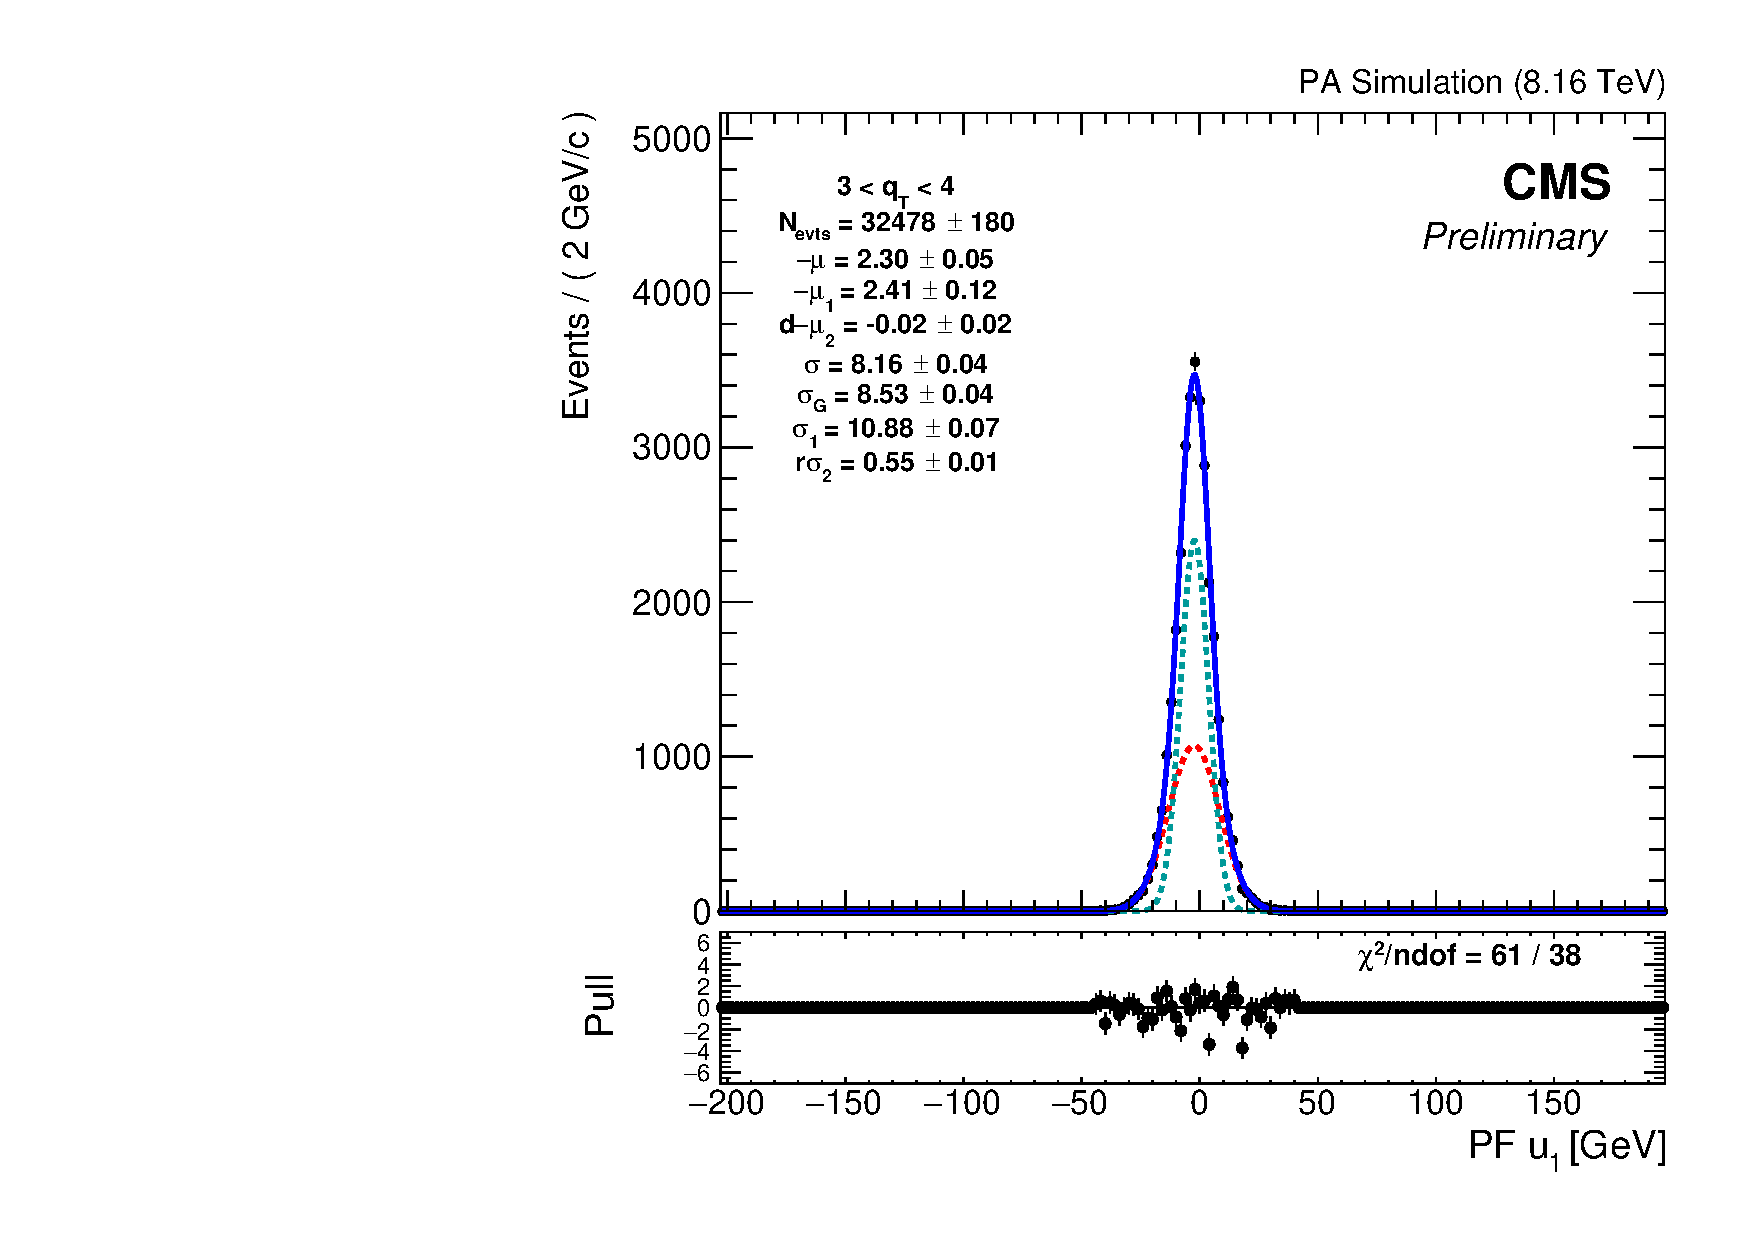
\includegraphics[width=0.4\textwidth]{Figures/WBoson/Analysis/Correction/Recoil/RecoilFits/MC/pfu1fit_2.pdf} \\
 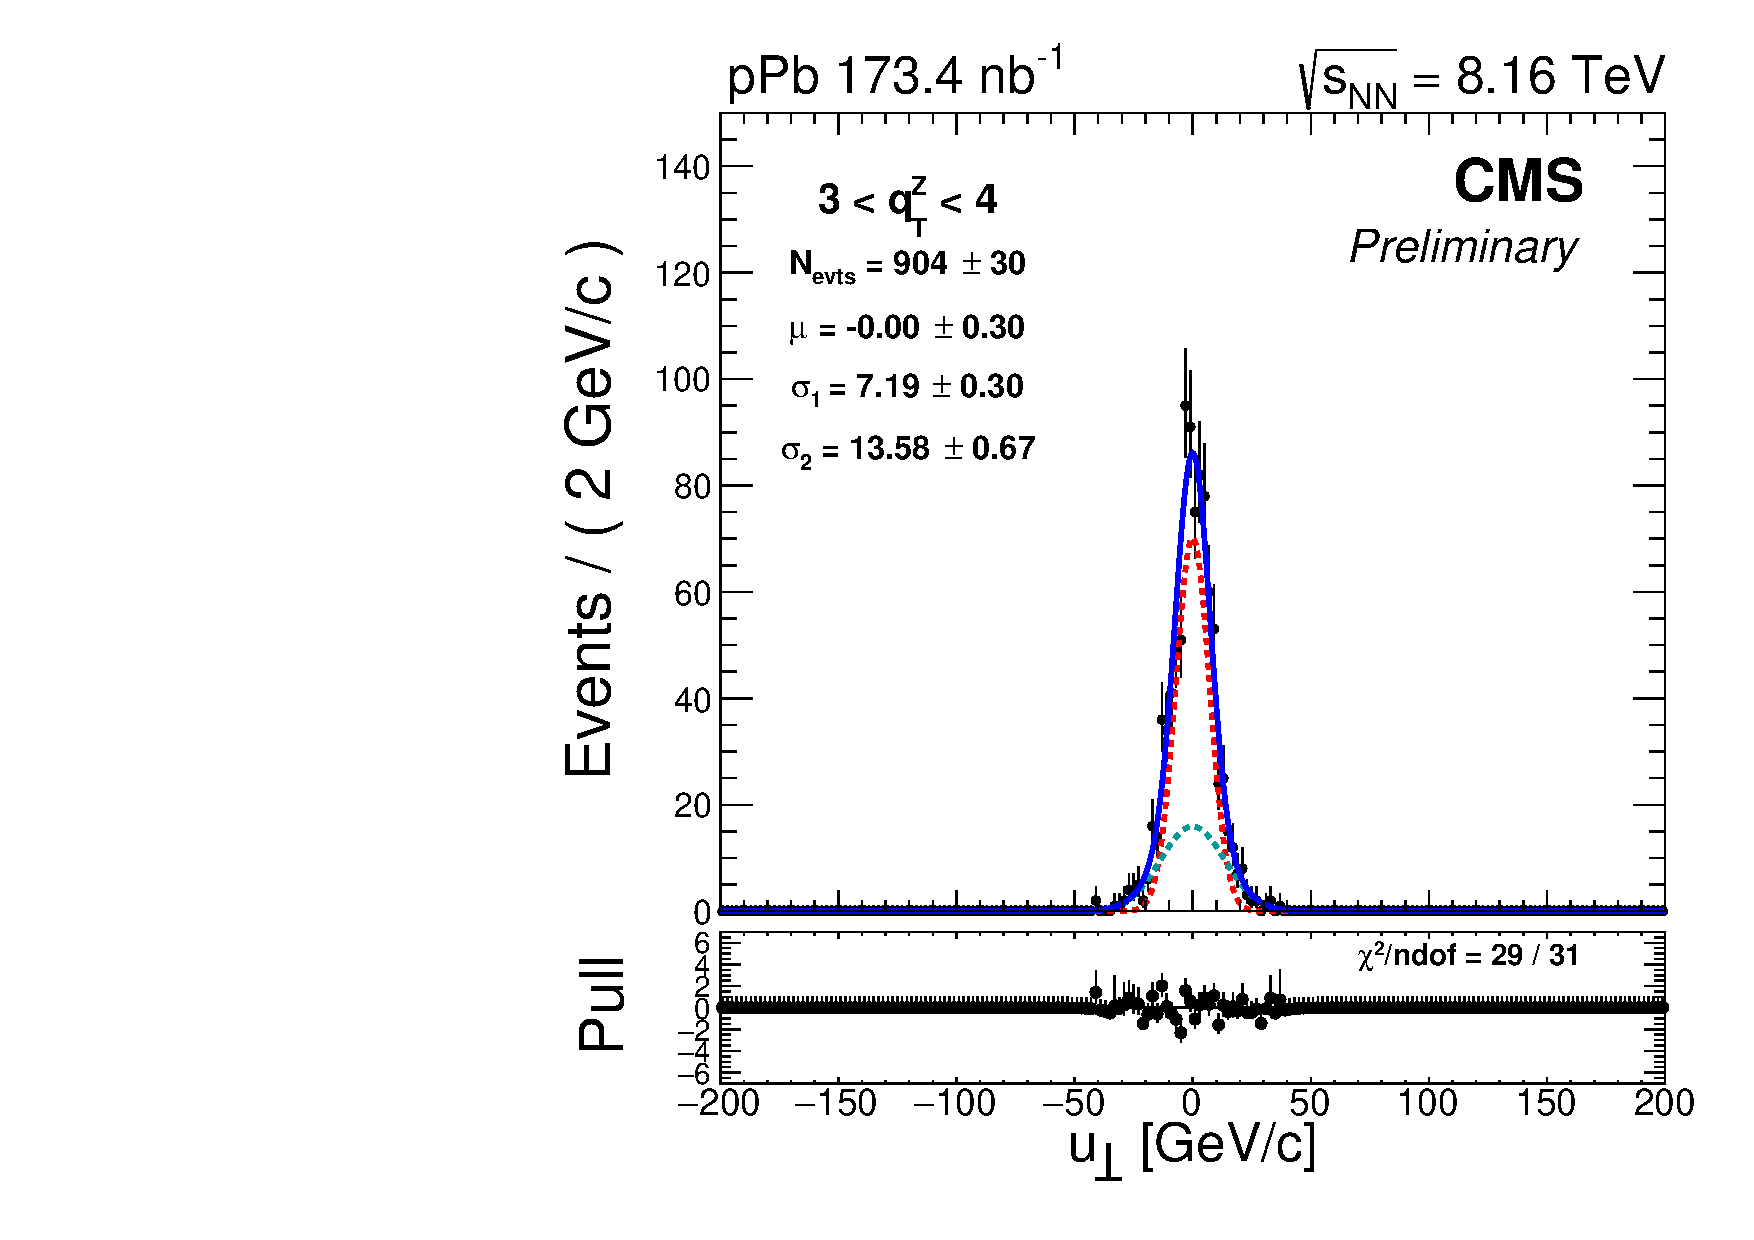
\includegraphics[width=0.4\textwidth]{Figures/WBoson/Analysis/Correction/Recoil/RecoilFits/Data/pfu2fit_2.pdf}
 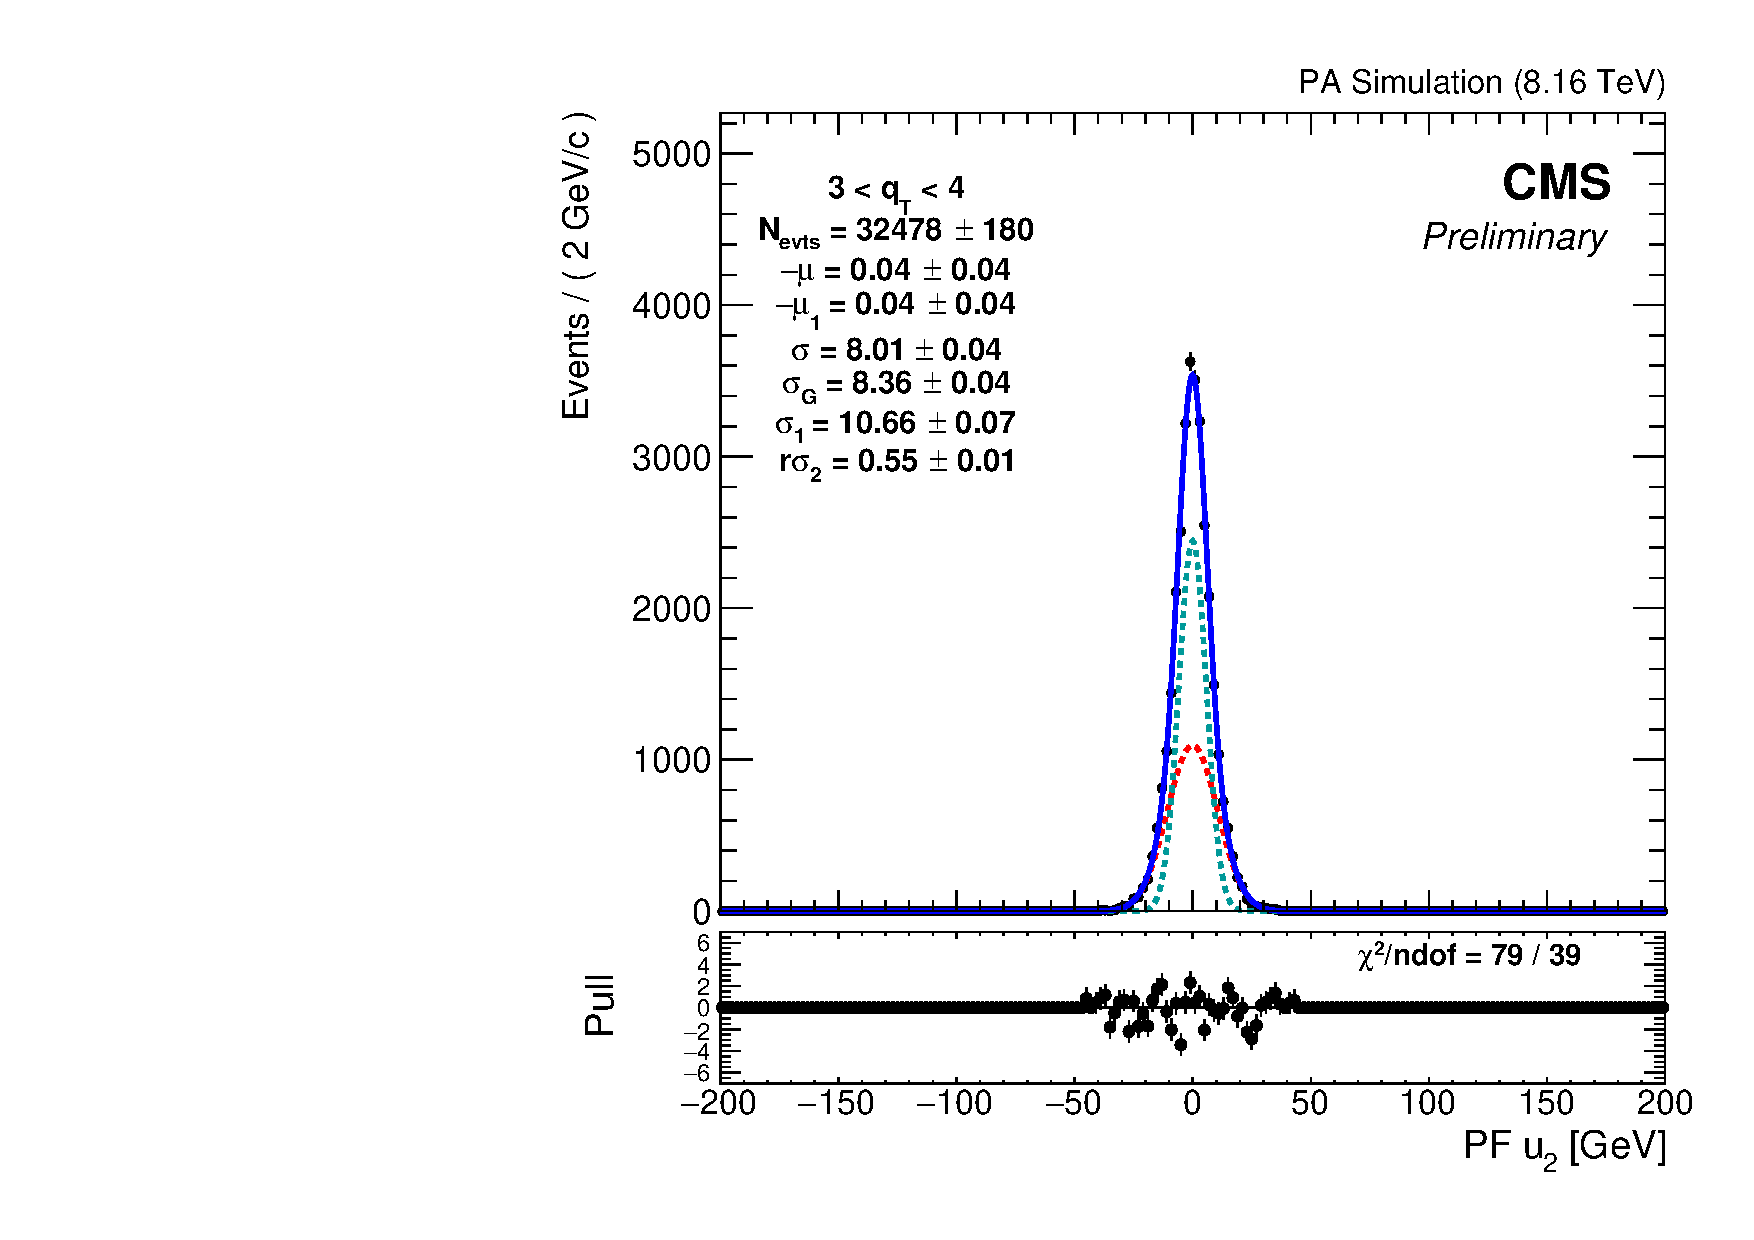
\includegraphics[width=0.4\textwidth]{Figures/WBoson/Analysis/Correction/Recoil/RecoilFits/MC/pfu2fit_2.pdf}
 \caption{Distributions of the \utpar (top) and \utper (bottom) recoil components in data (left) and simulation (right). The fit function is based on a weighted sum of two Gaussian distributions as defined in  in \eq{eq:gaussFit}. The plots correspond to the \qtZ bin [3, 4]~\GeVc.}
 \label{fig:RecoilFits}
\end{figure}

\paragraph{Parameterisation of the recoil scale.} The Gaussian mean parameter $\mu_{\parallel}$ of the recoil parallel component is extracted in each \qtZ bin by fitting the recoil \utper distribution as shown in \fig{fig:RecoilFits}. The profile of $\mu_{\parallel}$ as a function of \qtZ is then fitted using the following function: 

\begin{equation} 
 \mu_{\parallel}\left(\qtZ\right) = -\left(c_{0} + c_{1}\qtZ\right)\left(\frac{1 + \text{Erf}\left[\alpha{\cdot}\left(\qtZ\right)^{\beta}\right]}{2}\right)
 \label{eq:equparparam}
\end{equation}

where $c_{0}$, $c_{1}$, $\alpha$ and $\beta$ are free parameters, and $\text{Erf}(x)$ is the Gaussian error function. These fits are shown in \fig{fig:figU1RecoilScaleFit}, where the sign of $\mu_{\parallel}$ has been reversed to plot the results in the positive y-axis. The slope $c_{1}$ and intercept $c_{0}$ parameters are found to be $c_{1}{\approx}0.9$ and $c_{0}<1.0$~\GeVc, which means that the average \utpar is roughly $10\%$ lower than \qtZ and the contributions at $\qtZ=0$ are negligible. The distributions of the average \utpar for data and simulation are observed to be in good agreement.

\begin{figure}[htb!]
 \centering
 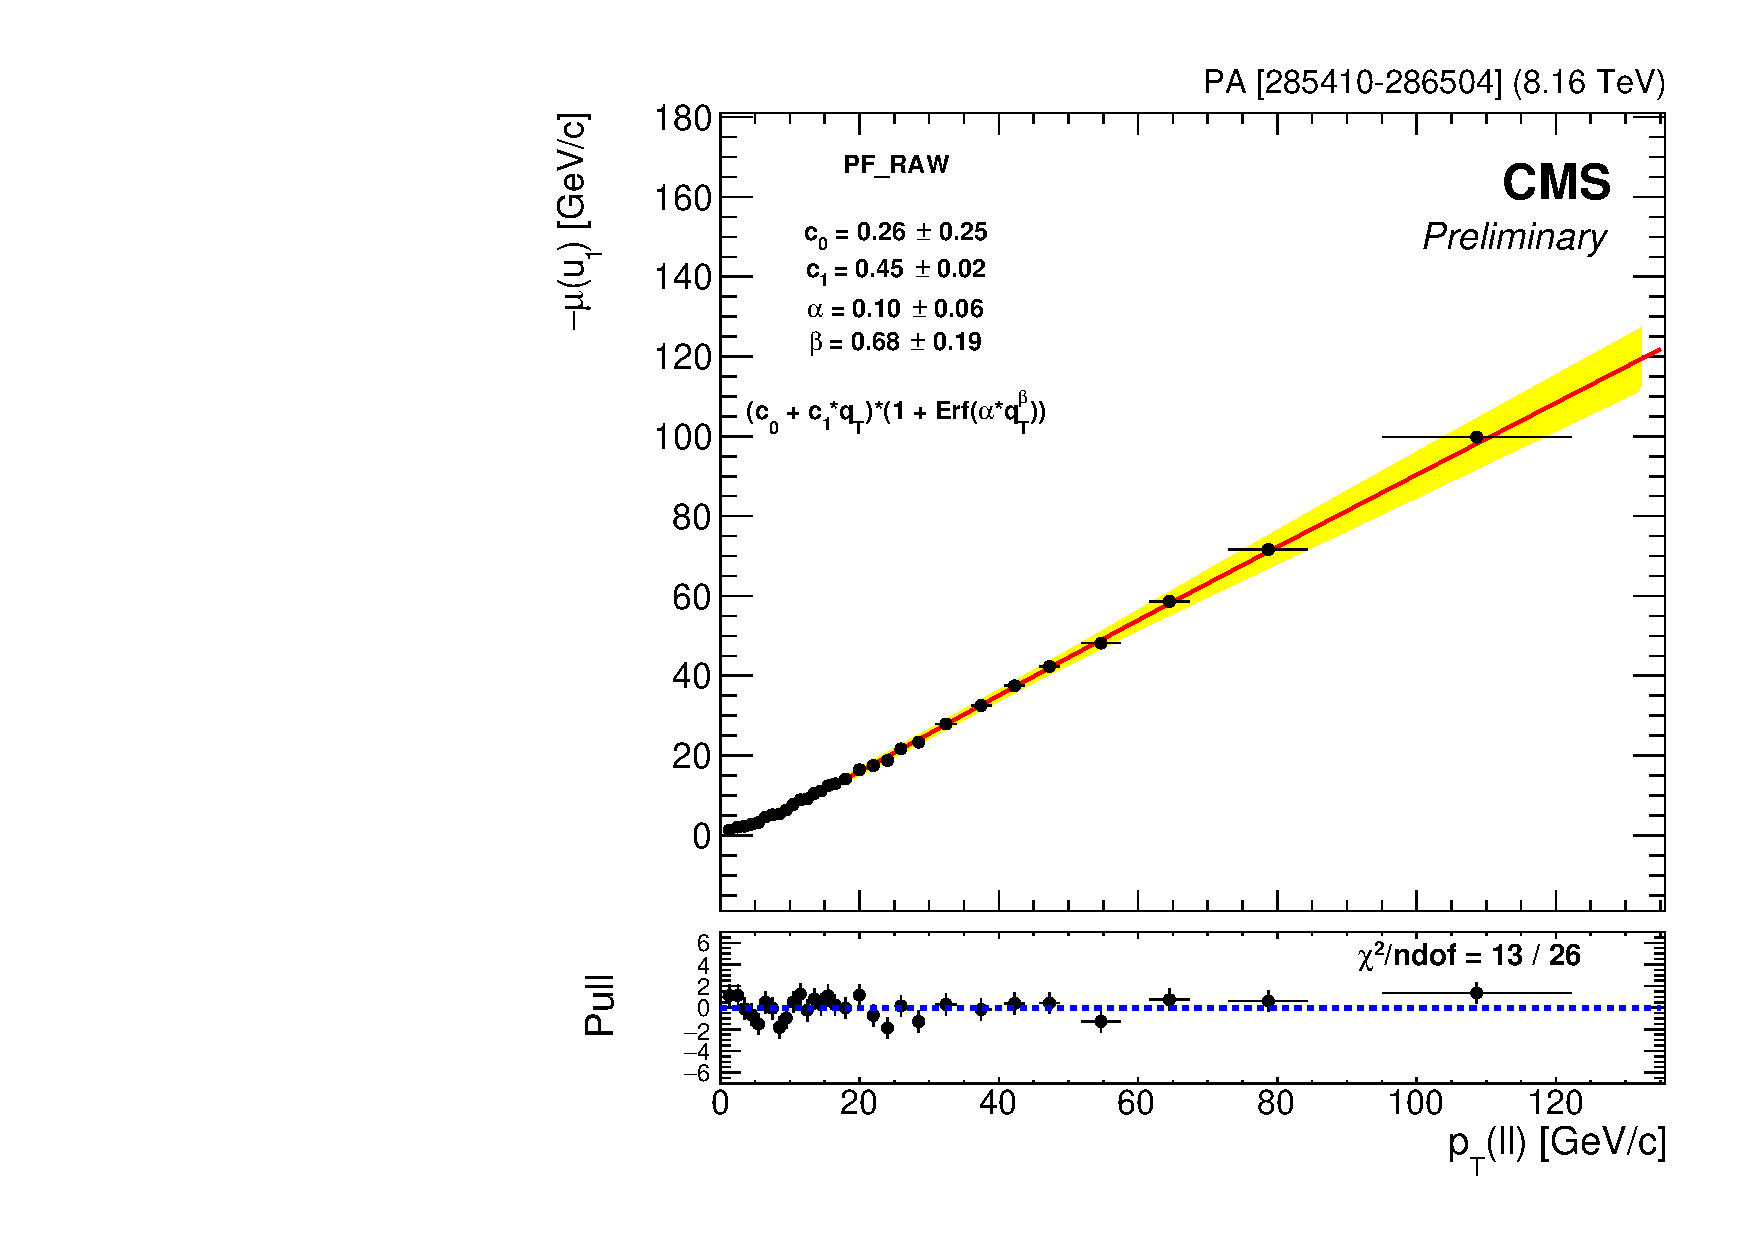
\includegraphics[width=0.45\textwidth]{Figures/WBoson/Analysis/Correction/Recoil/RecoilFitsqT/Data/fitPFu1mean.pdf}
 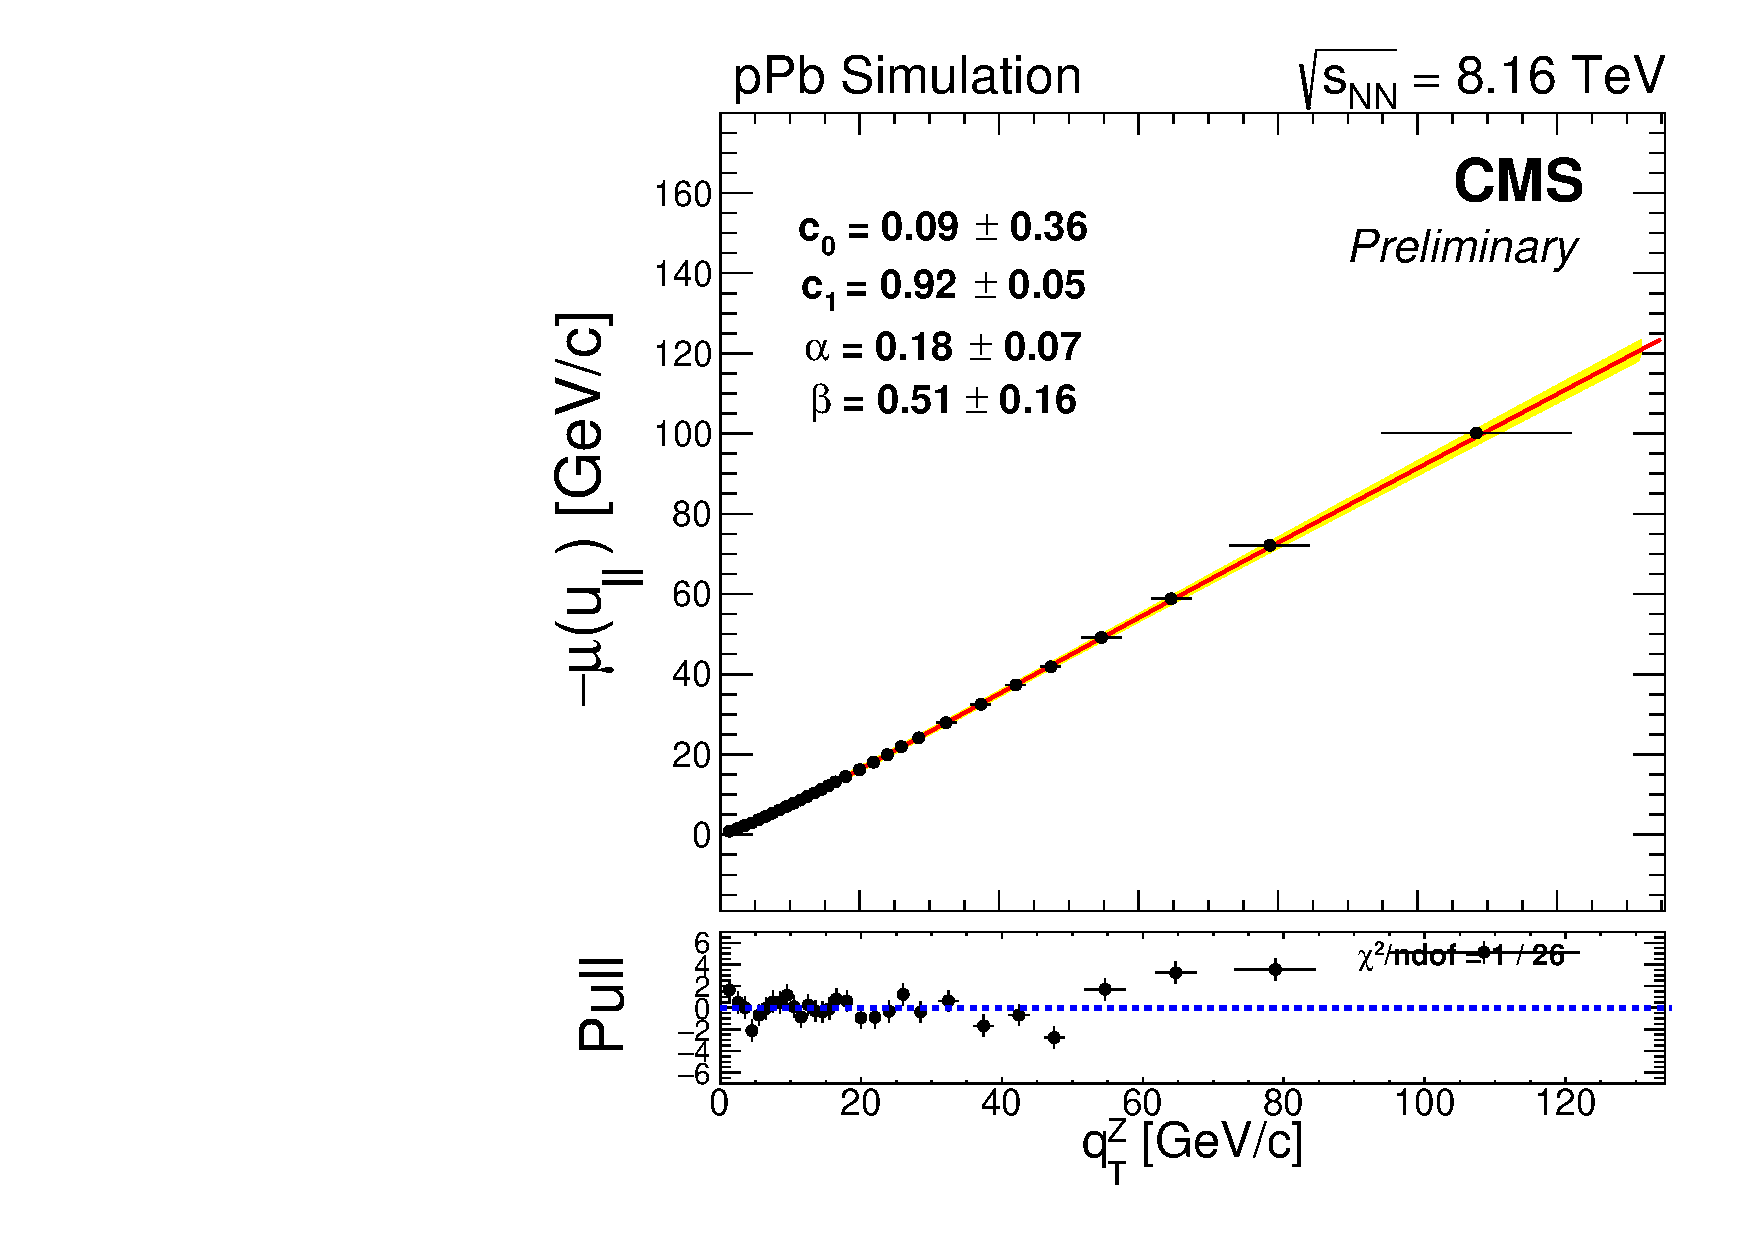
\includegraphics[width=0.45\textwidth]{Figures/WBoson/Analysis/Correction/Recoil/RecoilFitsqT/MC/fitPFu1mean.pdf}
 \caption{Fits of the profile of $-\mu_{\parallel}$ as a function of \qtZ. The results are derived from \ZToMuMu events in data (left) and simulation (right). The yellow band represents the 68\% error band of the  fit.}
 \label{fig:figU1RecoilScaleFit}
\end{figure}

In the case of the perpendicular recoil component, the average \utper value should be zero based on momentum conservation. To check this, the profile of the Gaussian mean parameter $\mu_{\perp}$ as a function of \qtZ is fitted in data and simulation with a constant function:

\begin{equation}
 \mu_{\perp}\left(\qtZ\right) = c_{0}
\end{equation}
 
The outcome of the fits is shown in \fig{fig:figU2RecoilScaleFit}. As expected, the $\mu_{\perp}$ is found to be consistent with zero in simulation and data, showing that there is no bias that affects the average value of the recoil component perpendicular to \qtZvec. From now on, $\mu_{\perp}$ is fixed to zero.

\begin{figure}[htb!]
 \centering
 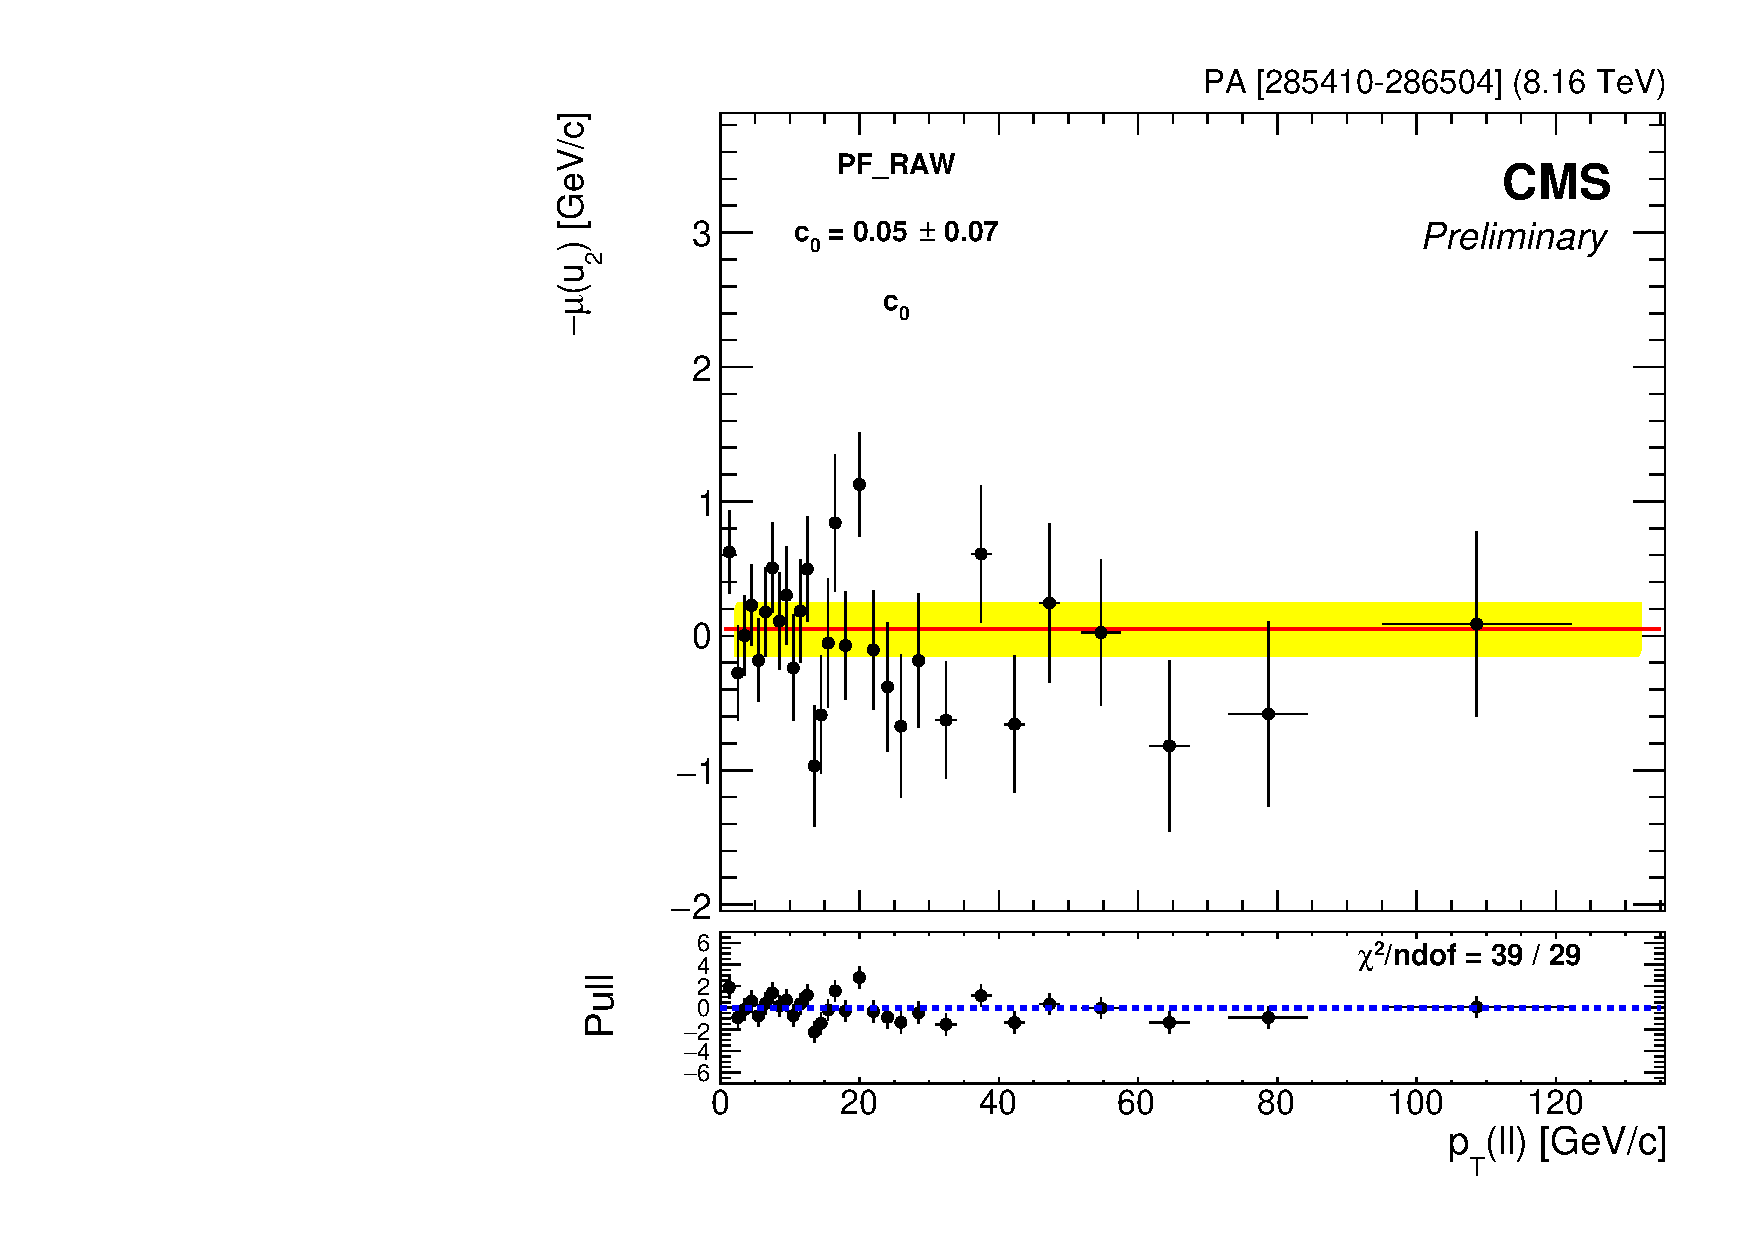
\includegraphics[width=0.45\textwidth]{Figures/WBoson/Analysis/Correction/Recoil/RecoilFitsqT/Data/fitPFu2mean.pdf}
 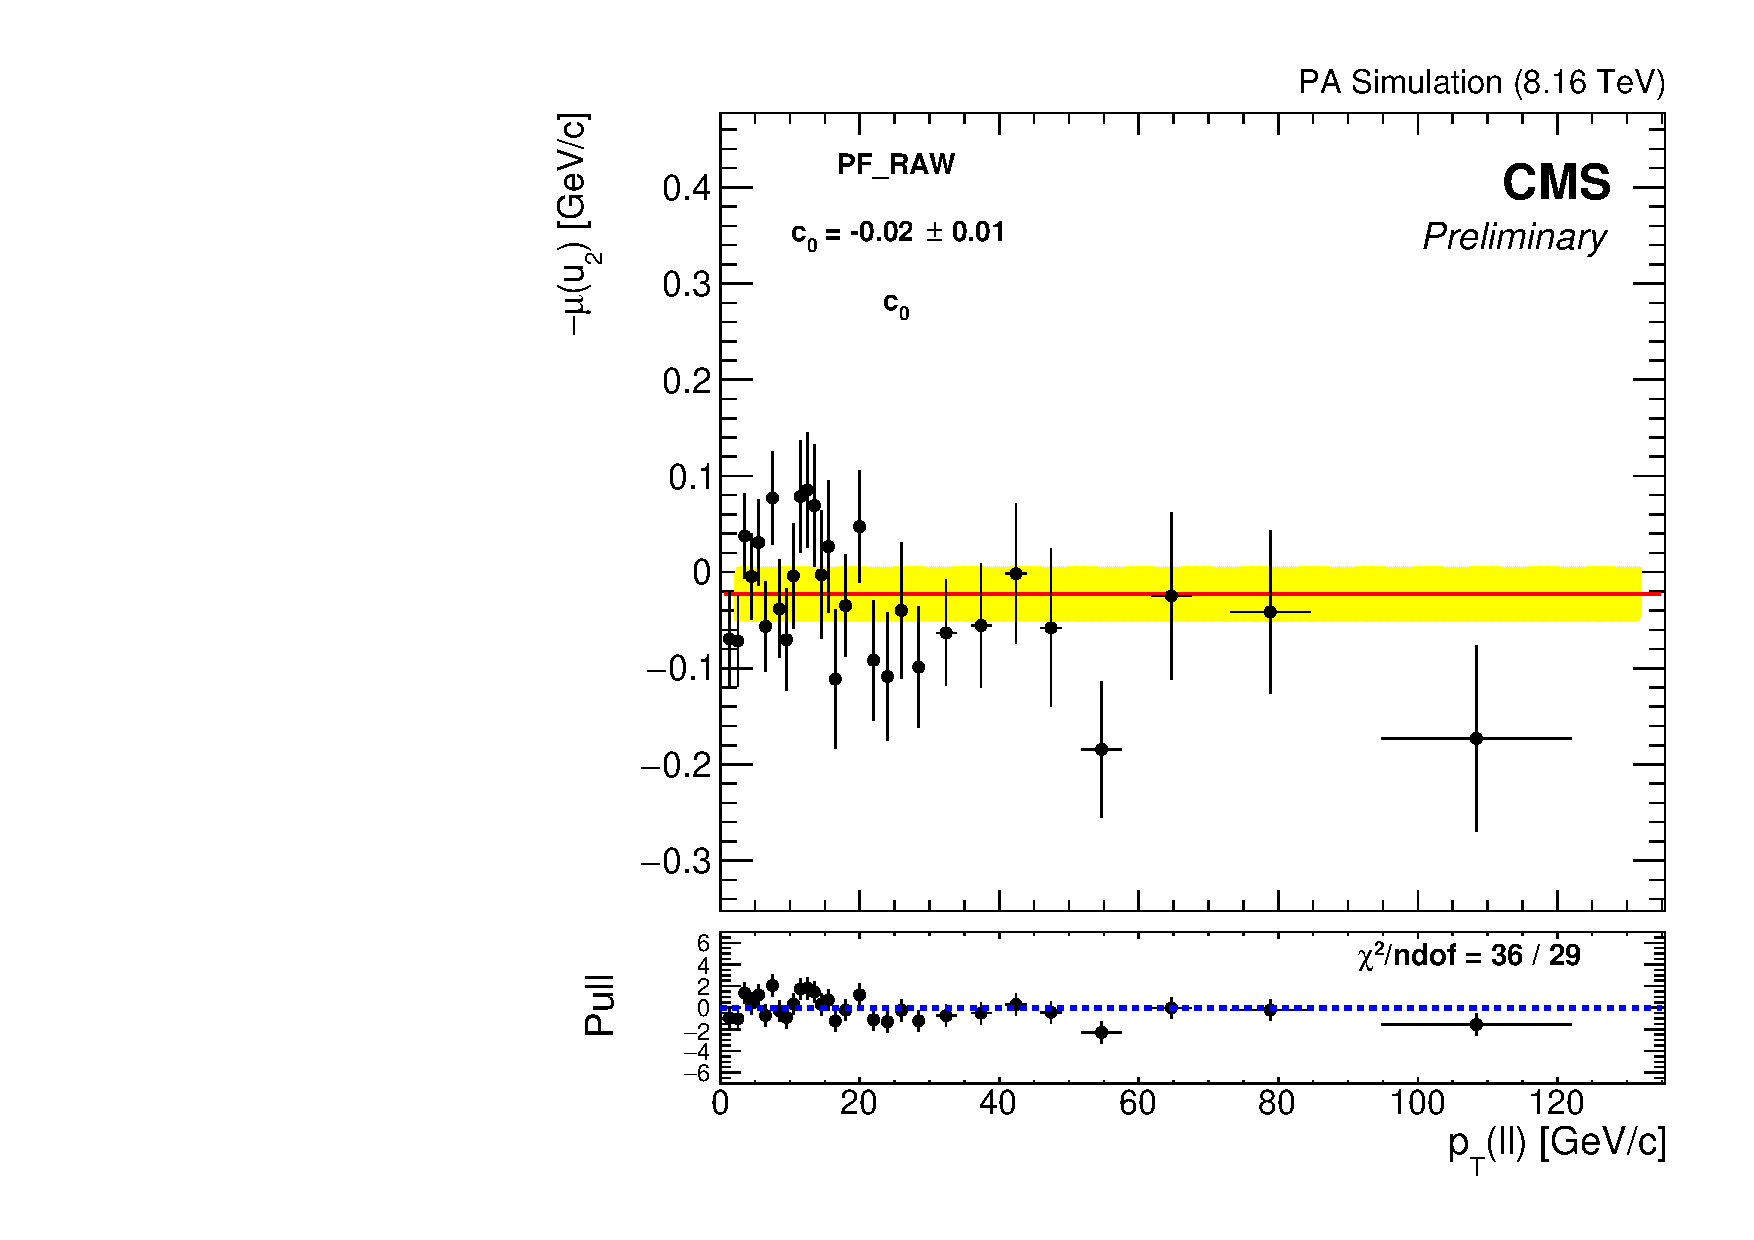
\includegraphics[width=0.45\textwidth]{Figures/WBoson/Analysis/Correction/Recoil/RecoilFitsqT/MC/fitPFu2mean.pdf}
 \caption{Fits of the profile of $\mu_{\perp}$ as a function of \qtZ. The results are derived from \ZToMuMu events in data (left) and simulation (right). The yellow band represents the 68\% error band of the fit.}
 \label{fig:figU2RecoilScaleFit}
\end{figure}

\paragraph{Parameterisation of the recoil resolution.} The two Gaussian width parameters ($\sigma_{\parallel(\perp),1}$ and $\sigma_{\parallel(\perp),2}$) of the parallel (perpendicular) component of the recoil are also extracted from the recoil fits for each \qtZ bin. The $\sigma_{\parallel(\perp),1}$ and $\sigma_{\parallel(\perp),2}$ parameters of \utpar (\utper) are parametrised as a function of \qtZ using the following formula:

\begin{equation}
 \sigma_{1,2}\left(\qtZ\right) = \sqrt{s_{0}^{2} + s_{1}^{2} \cdot q_{T}^{\alpha}}
 \label{eq:equreolnparam} 
\end{equation}

where $s_{0}$, $s_{1}$ and $\alpha$ are free parameters. The results of the fits to the $\sigma_{1}$ and $\sigma_{2}$ profiles as a function of \qtZ are presented in \fig{fig:figU1RecoilResolutionFit} for \utpar and in \fig{fig:figU2RecoilResolutionFit} for \utper. In addition, the profiles of the weighed average of the two Gaussian width parameters, given by:

\begin{equation}
 \begin{aligned}
  \sigma_{\perp} &= f_{\perp} \cdot \sigma_{\perp,1} + (1 - f_{\perp}) \cdot \sigma_{\perp,2} \\
  \sigma_{\parallel} &= f_{\parallel} \cdot \sigma_{\parallel,1} + (1 - f_{\parallel}) \cdot \sigma_{\parallel,2}
 \end{aligned}
 \label{eq:SigmaAvg} 
\end{equation}

are also fitted using \eq{eq:equreolnparam} and the results are shown in \fig{fig:figU2RecoilResolutionFit} and \fig{fig:figU1RecoilResolutionFit}.

\begin{figure}[htb!]
 \centering
 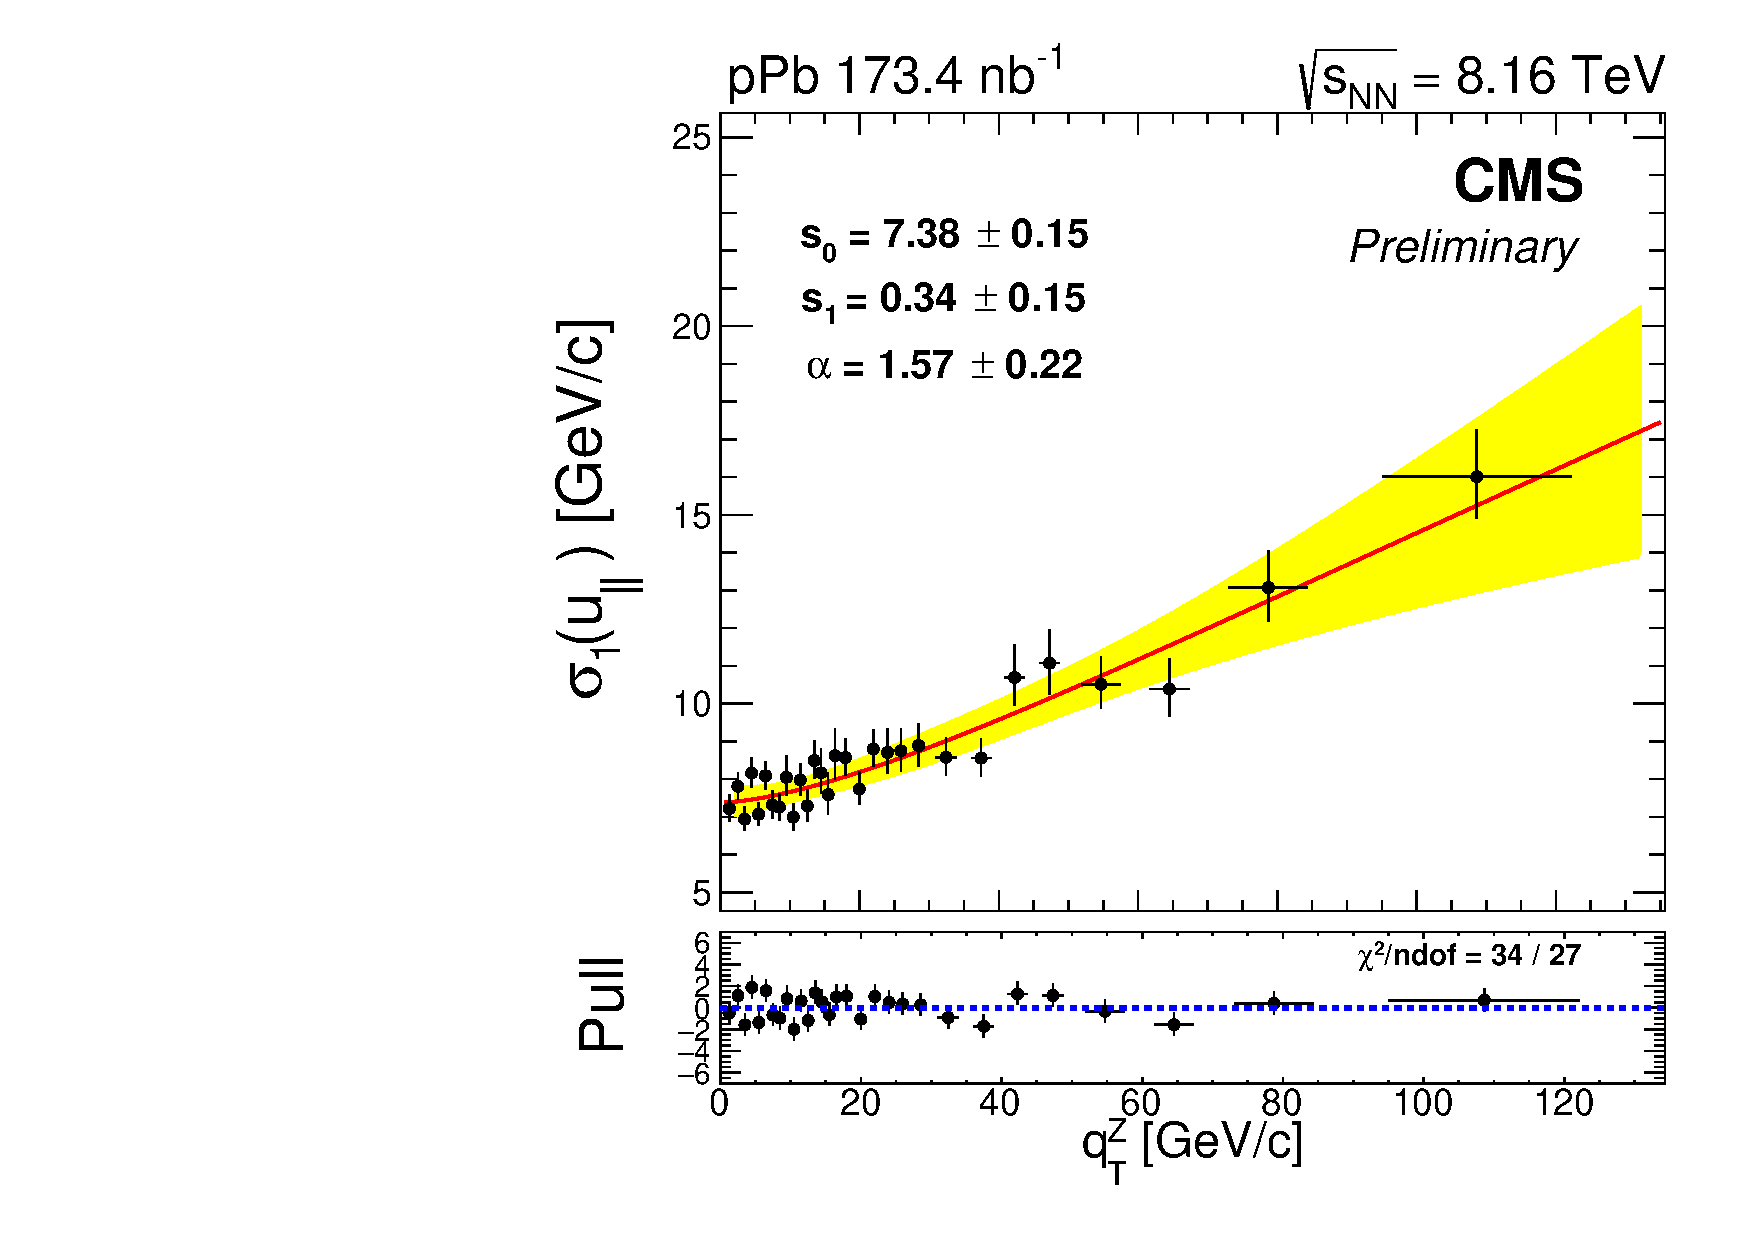
\includegraphics[width=0.3\textwidth]{Figures/WBoson/Analysis/Correction/Recoil/RecoilFitsqT/Data/fitPFu1sigma1.pdf}
 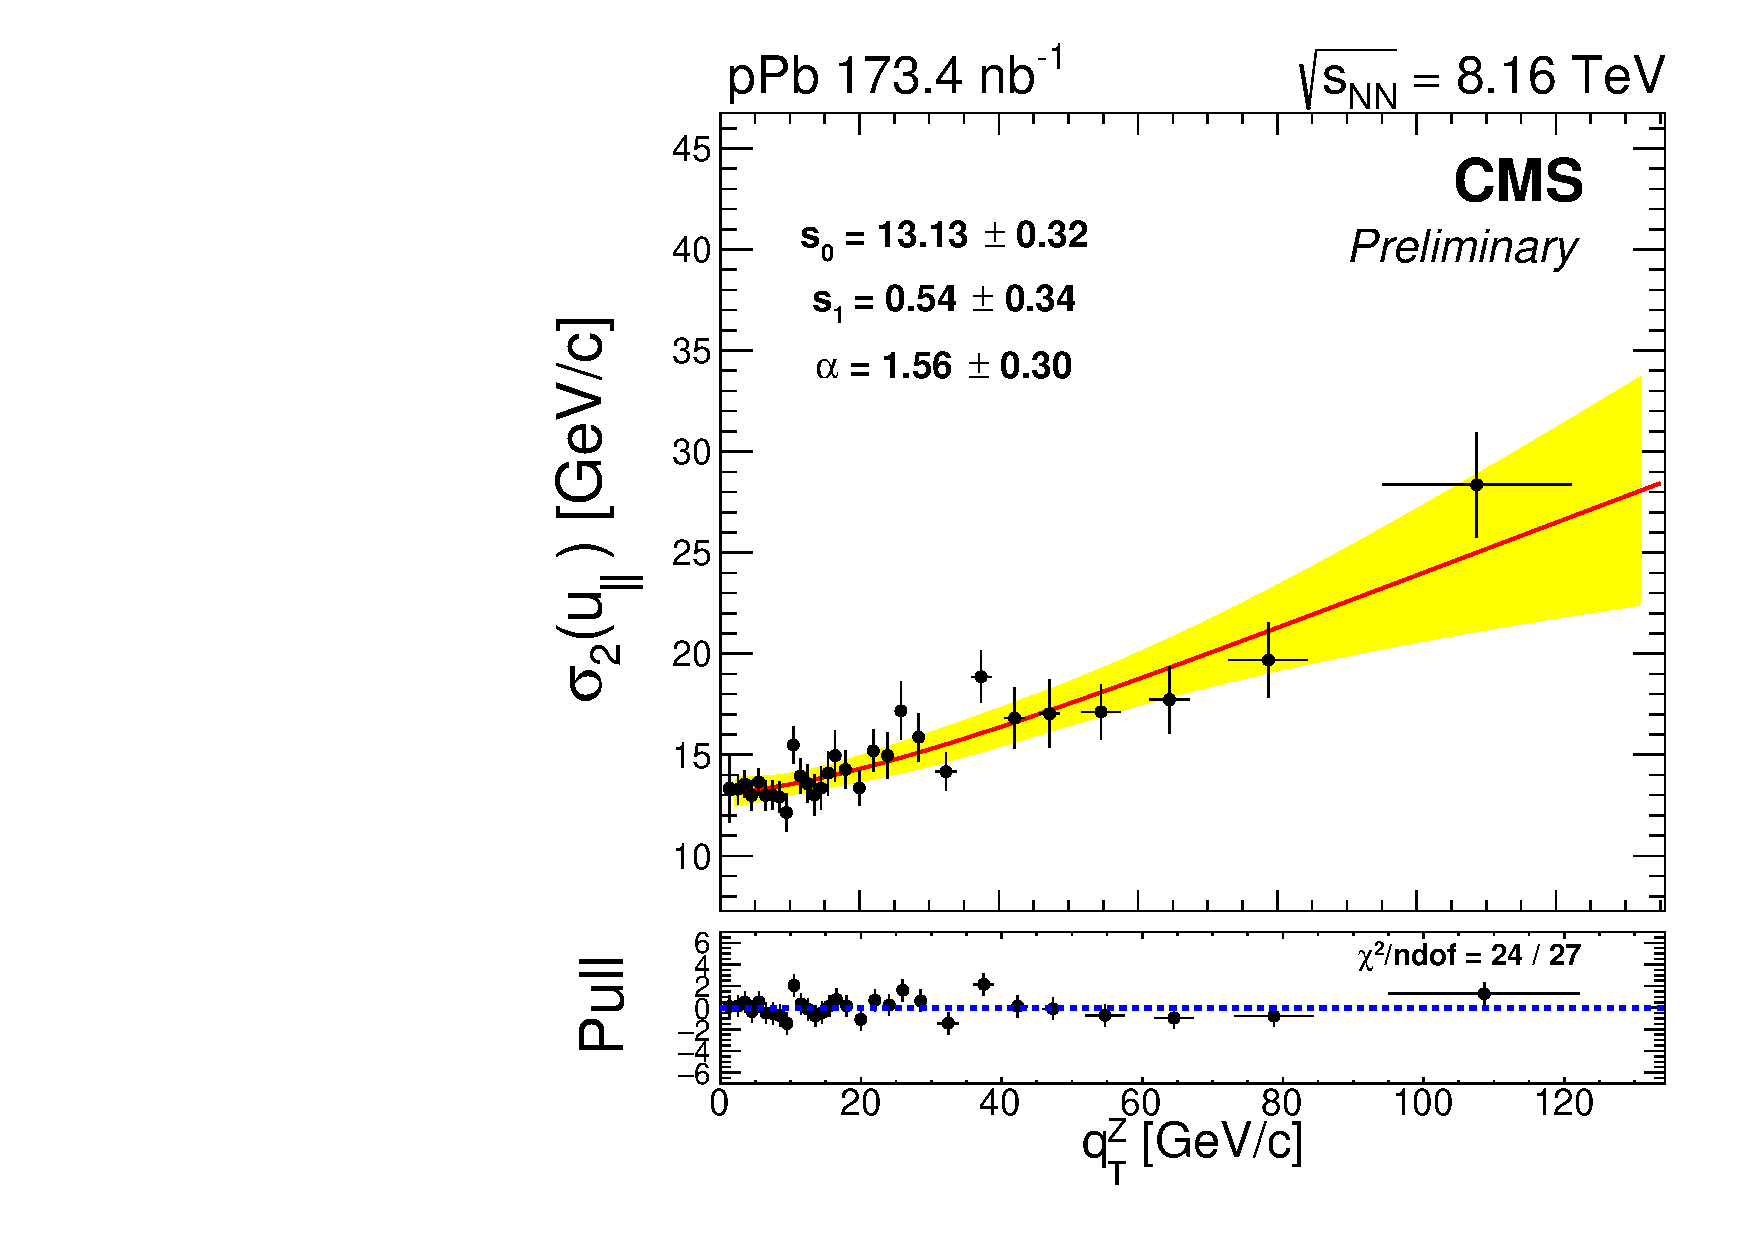
\includegraphics[width=0.3\textwidth]{Figures/WBoson/Analysis/Correction/Recoil/RecoilFitsqT/Data/fitPFu1sigma2.pdf}
 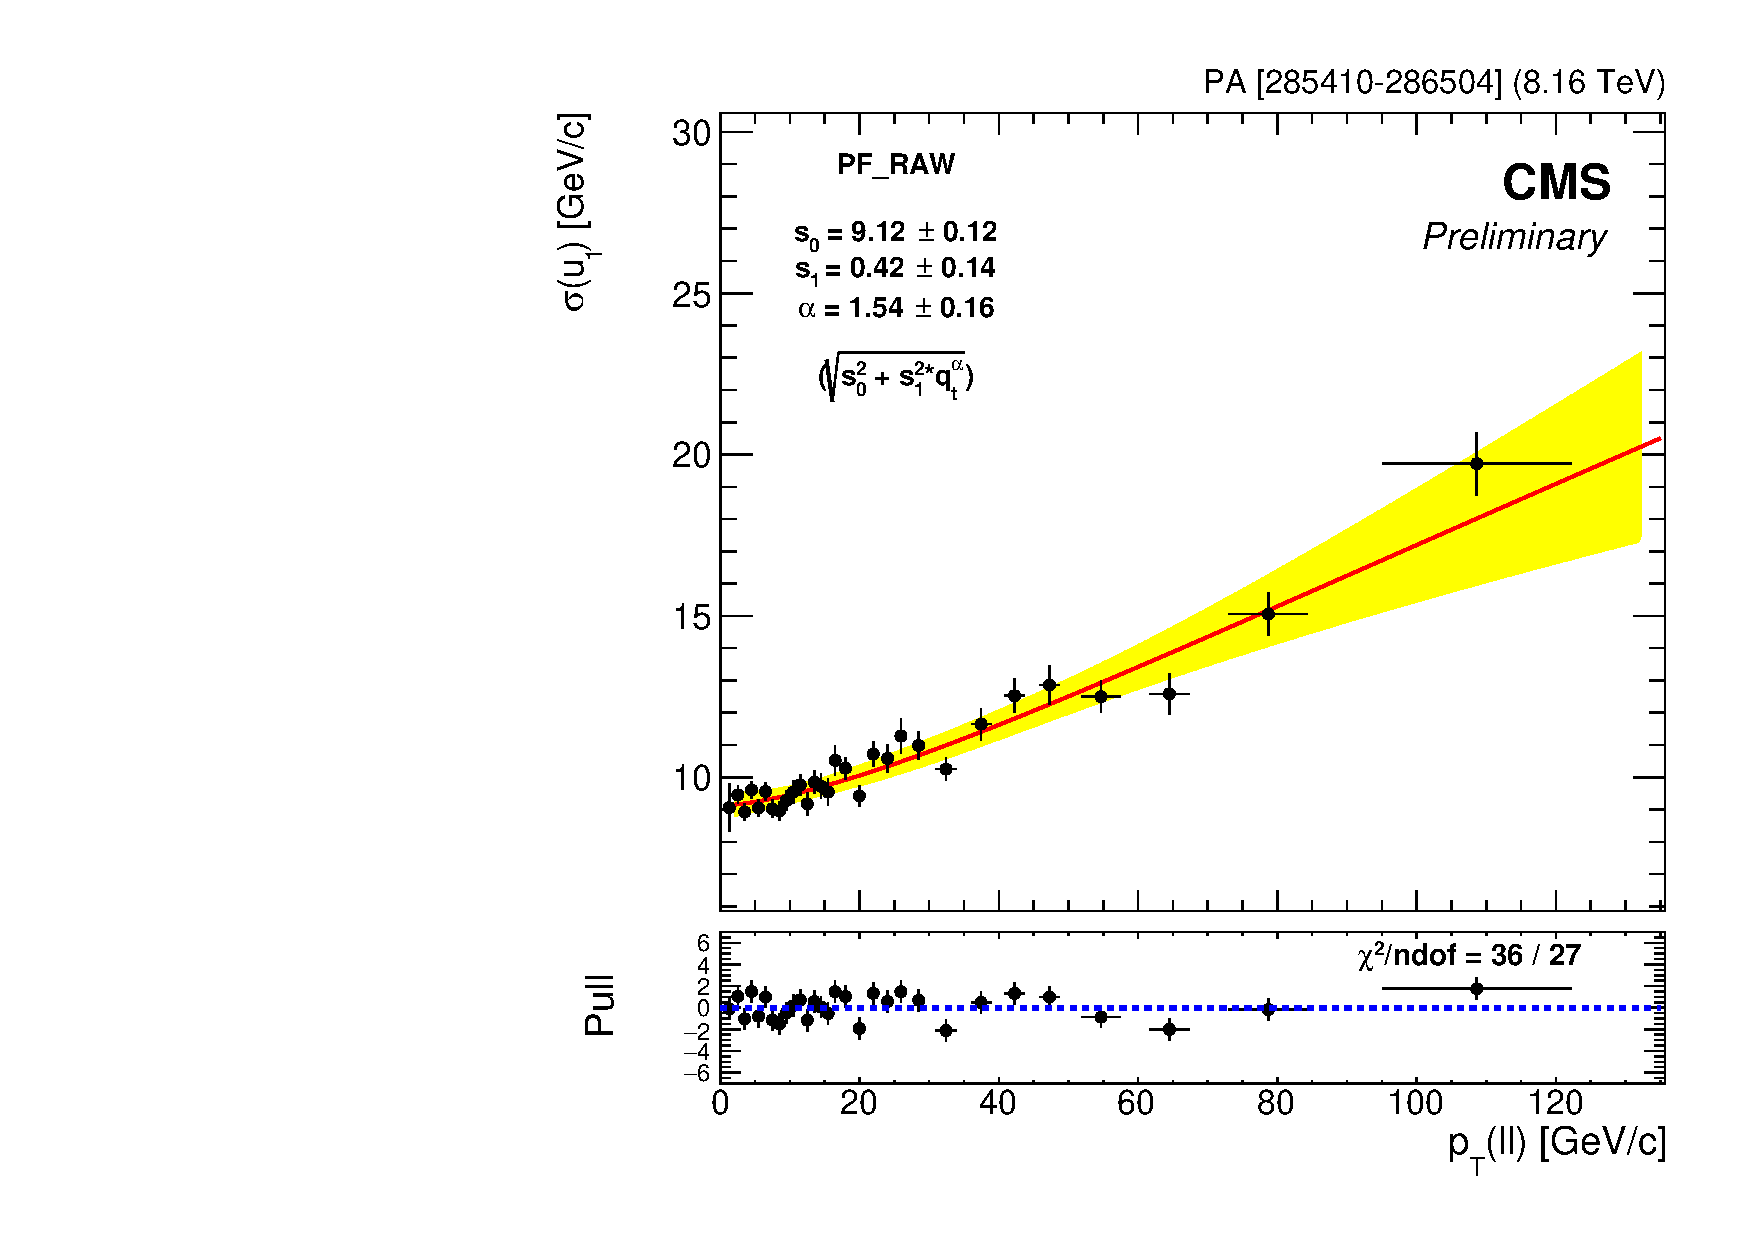
\includegraphics[width=0.3\textwidth]{Figures/WBoson/Analysis/Correction/Recoil/RecoilFitsqT/Data/fitPFu1sigma.pdf} \\
 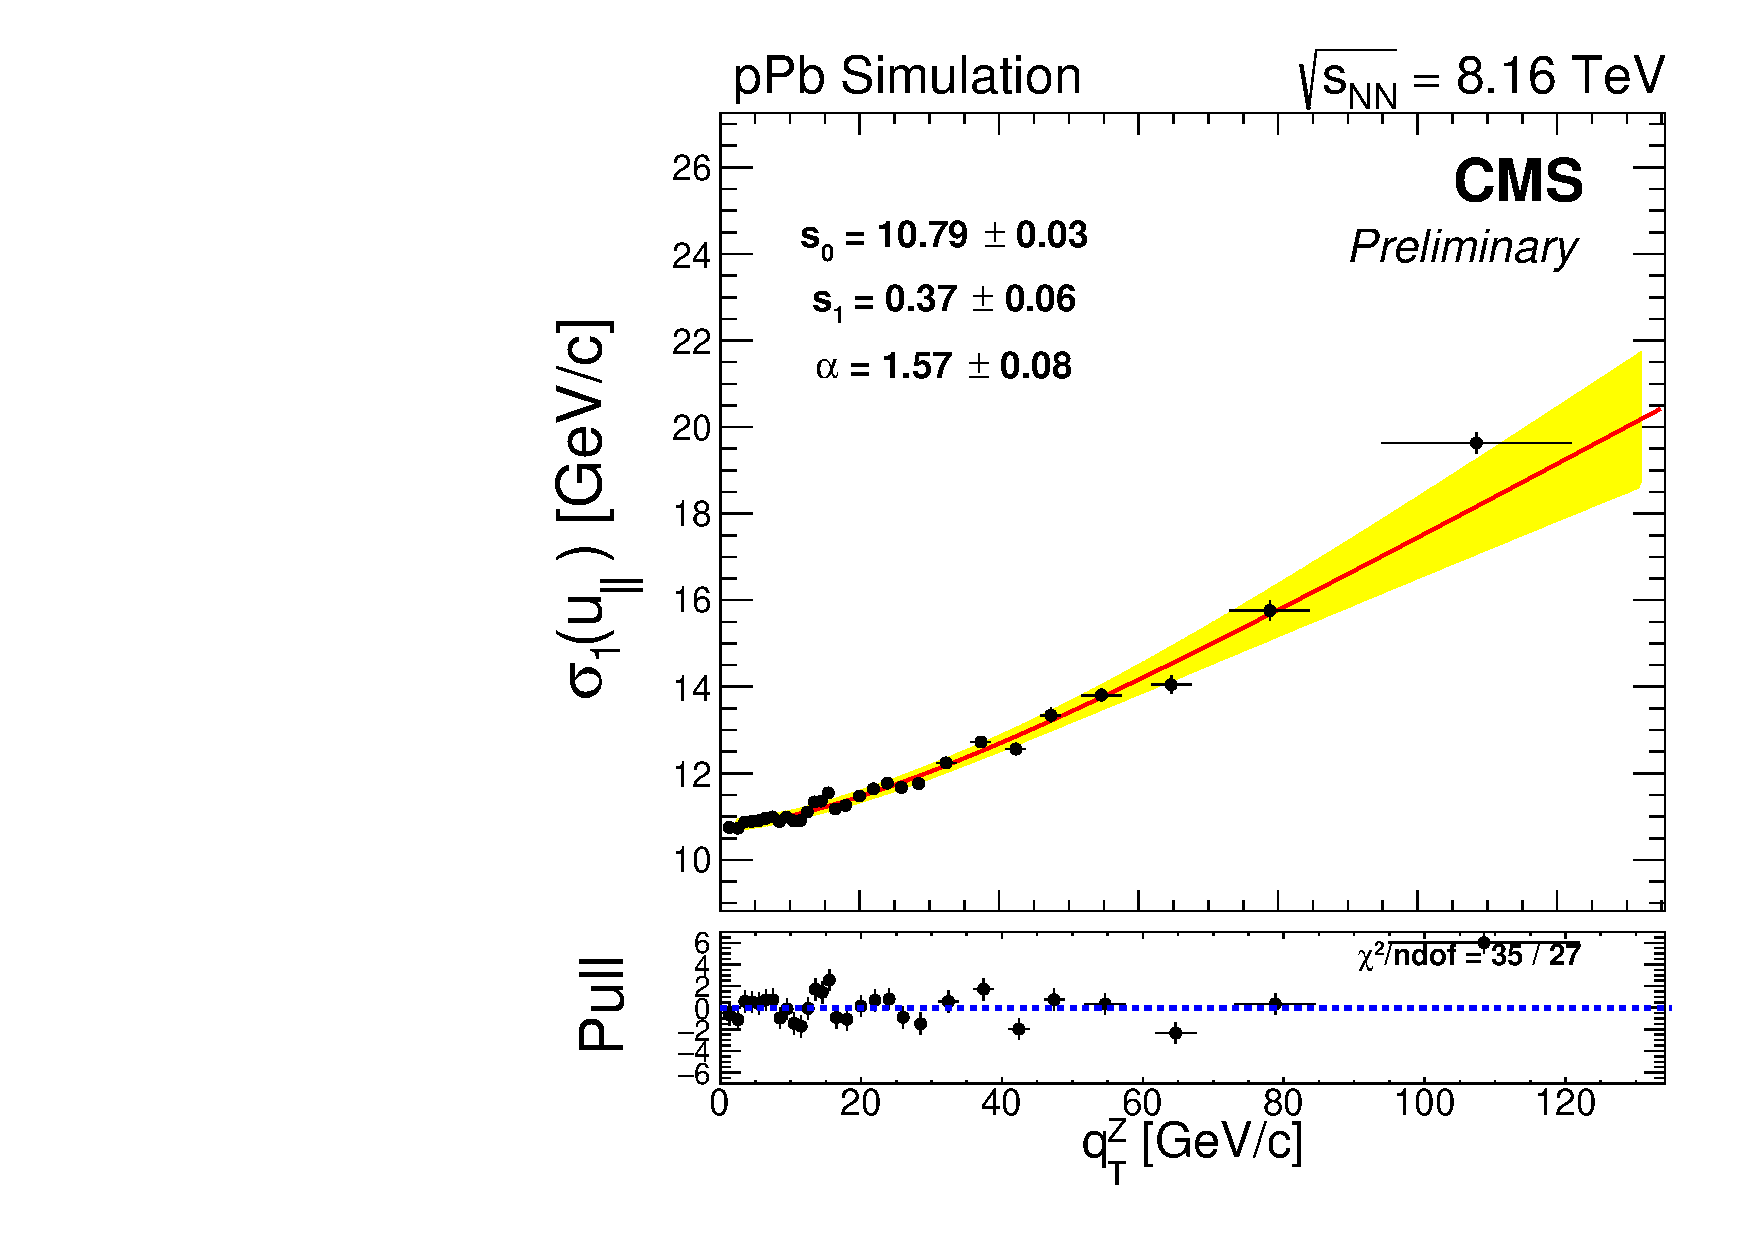
\includegraphics[width=0.3\textwidth]{Figures/WBoson/Analysis/Correction/Recoil/RecoilFitsqT/MC/fitPFu1sigma1.pdf}
 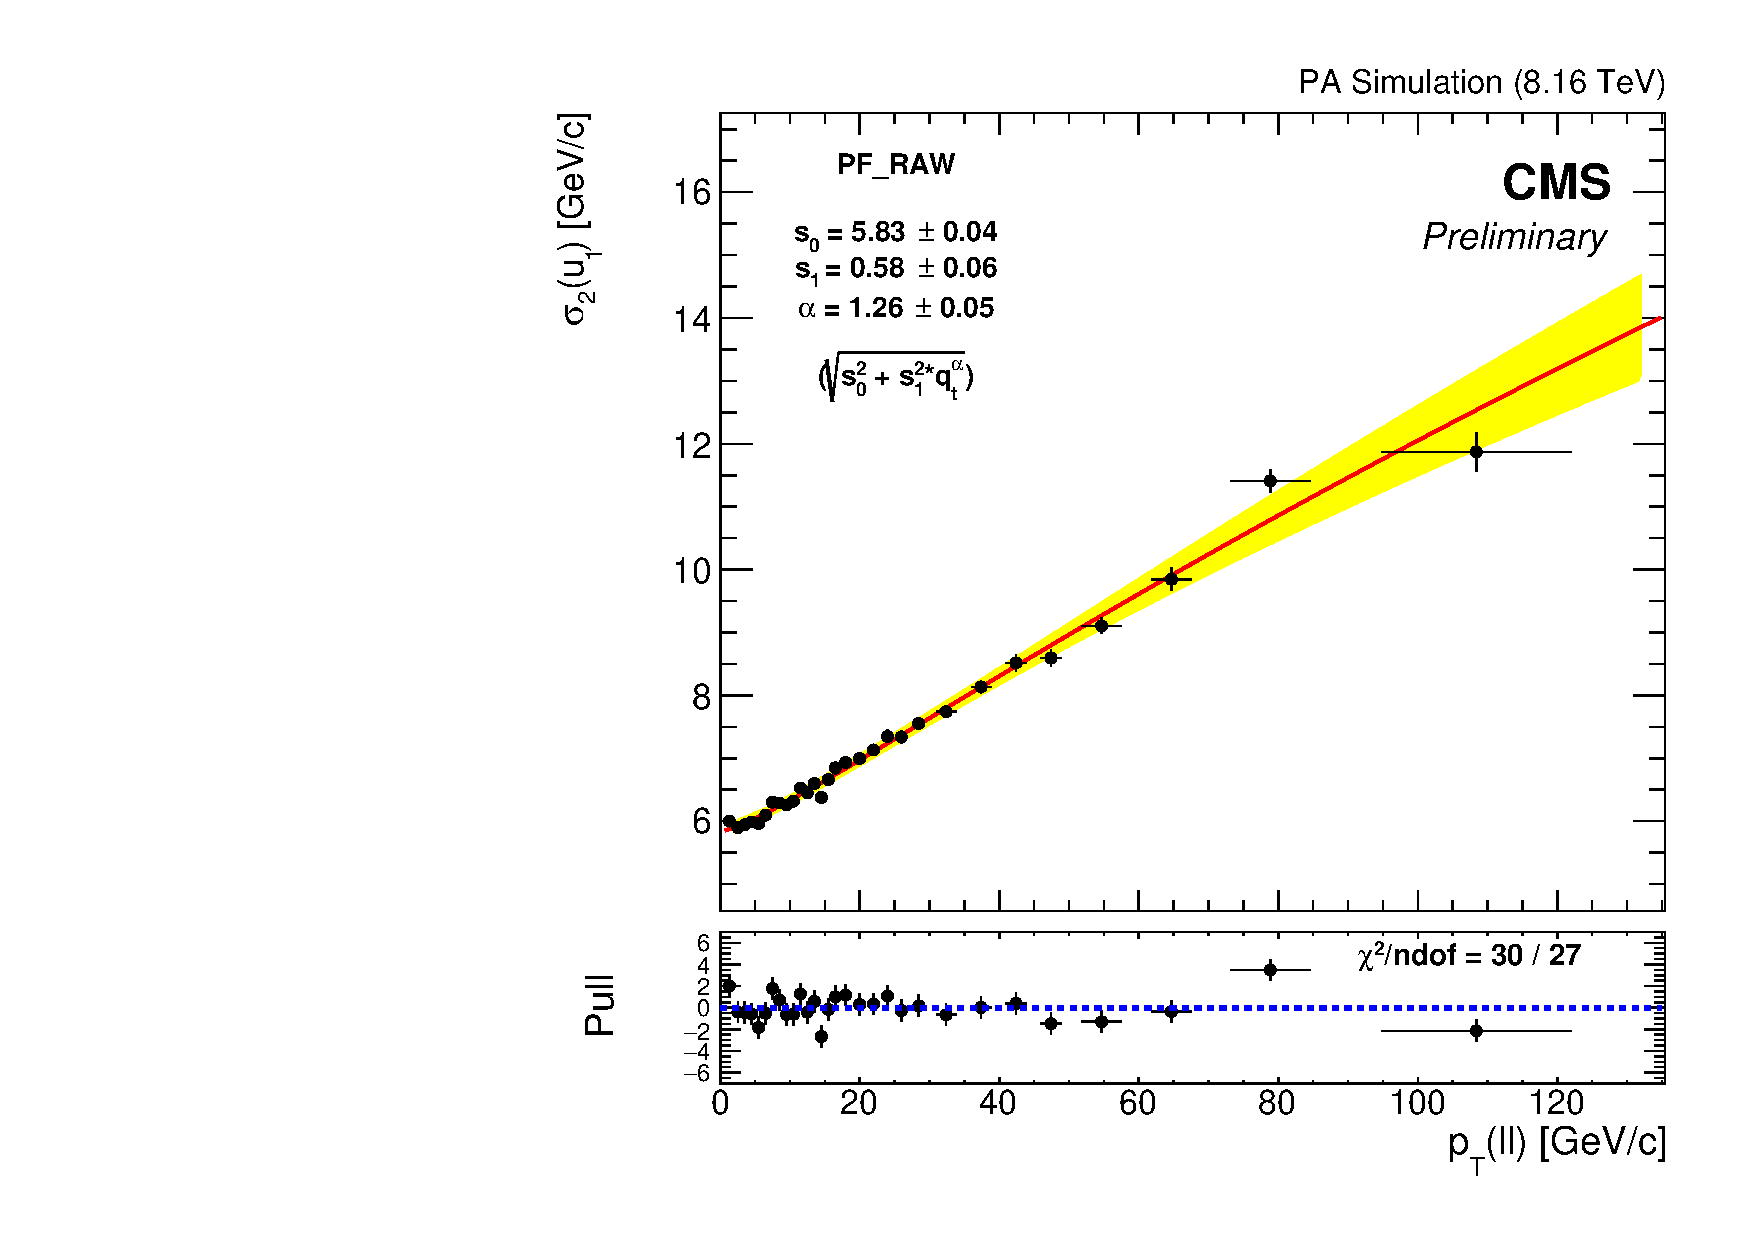
\includegraphics[width=0.3\textwidth]{Figures/WBoson/Analysis/Correction/Recoil/RecoilFitsqT/MC/fitPFu1sigma2.pdf}
 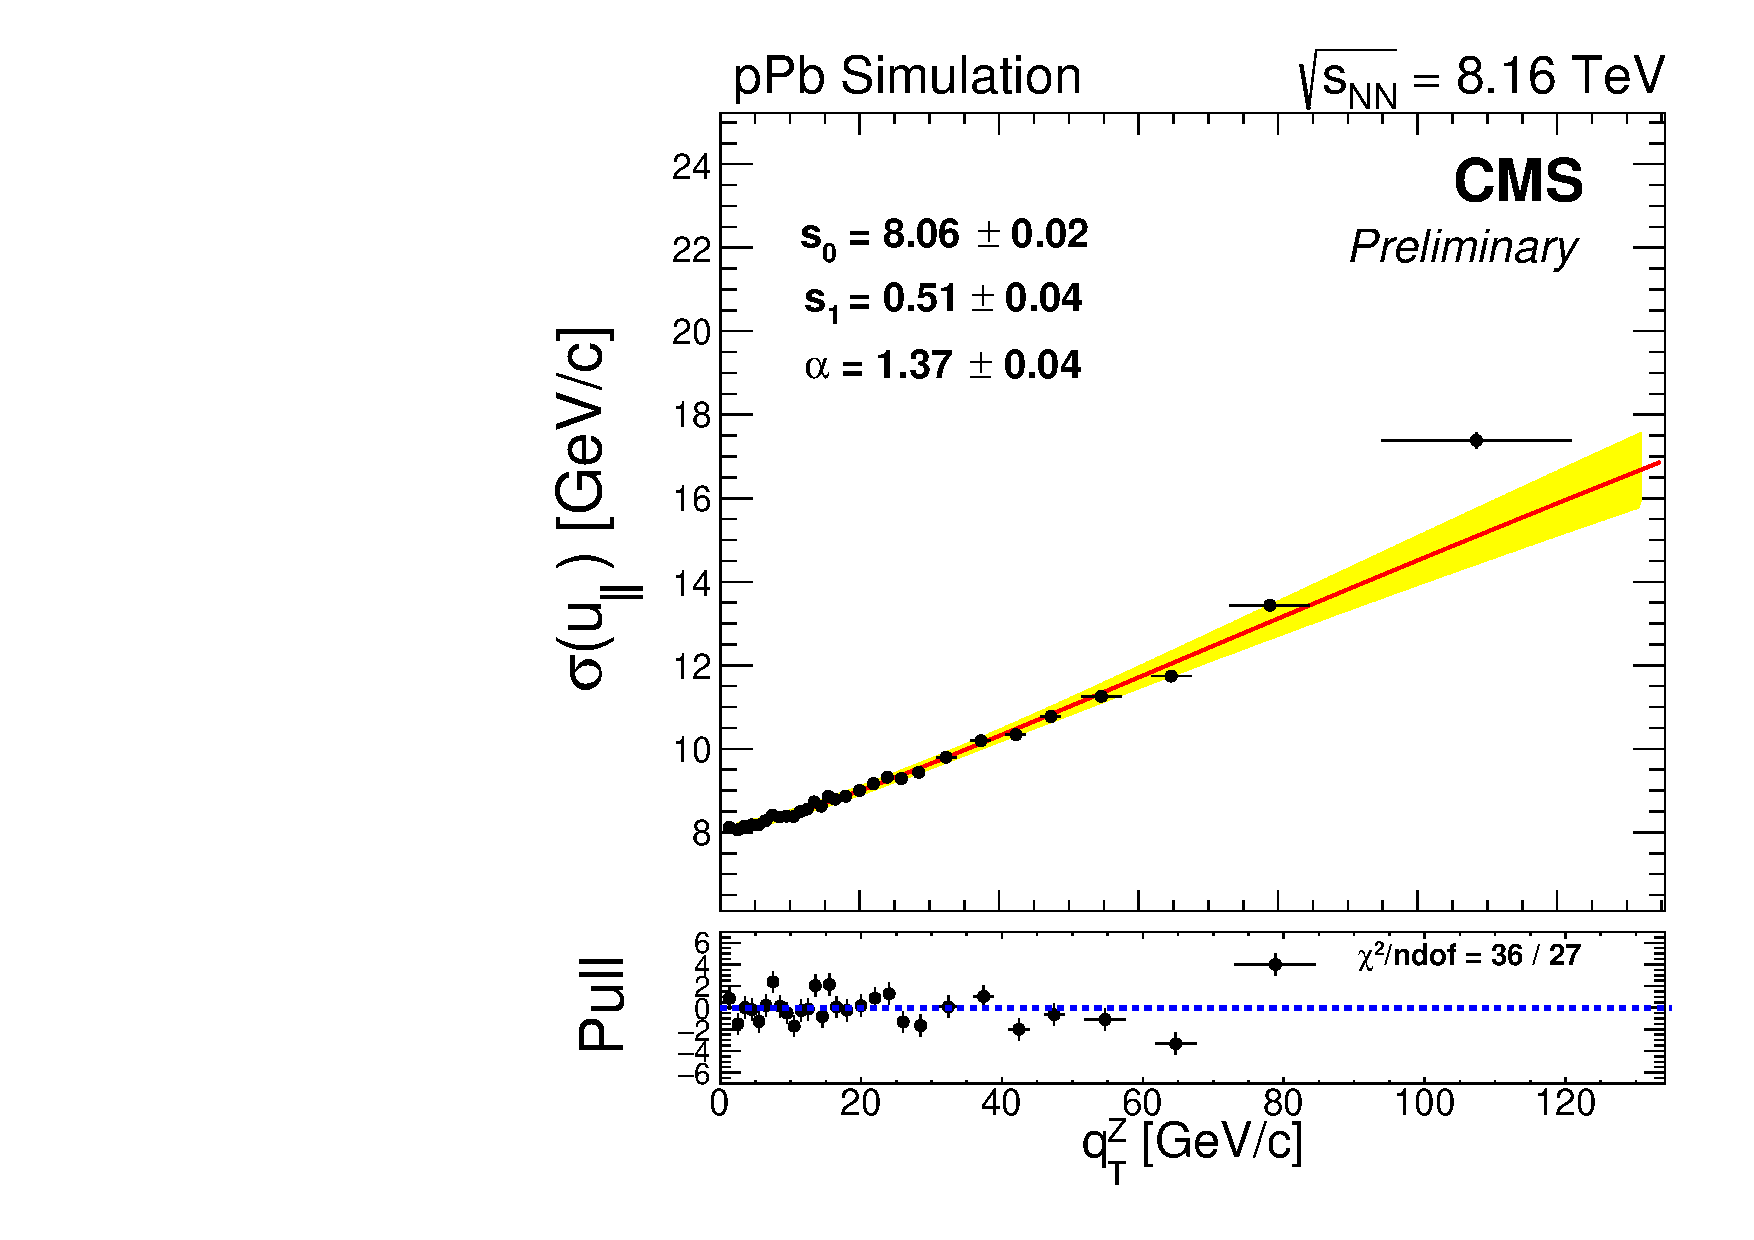
\includegraphics[width=0.3\textwidth]{Figures/WBoson/Analysis/Correction/Recoil/RecoilFitsqT/MC/fitPFu1sigma.pdf}
 \caption{Fits to the profile of the $\sigma_{\parallel,1}$ (left), $\sigma_{\parallel,2}$ (middle) and weighed average $\sigma_{\parallel}$ (right) values of the parallel recoil component as a function of \qtZ. . The results are derived from \ZToMuMu events in data (top) and simulation (bottom).}
 \label{fig:figU1RecoilResolutionFit}
\end{figure}

\begin{figure}[htb!]
 \centering
 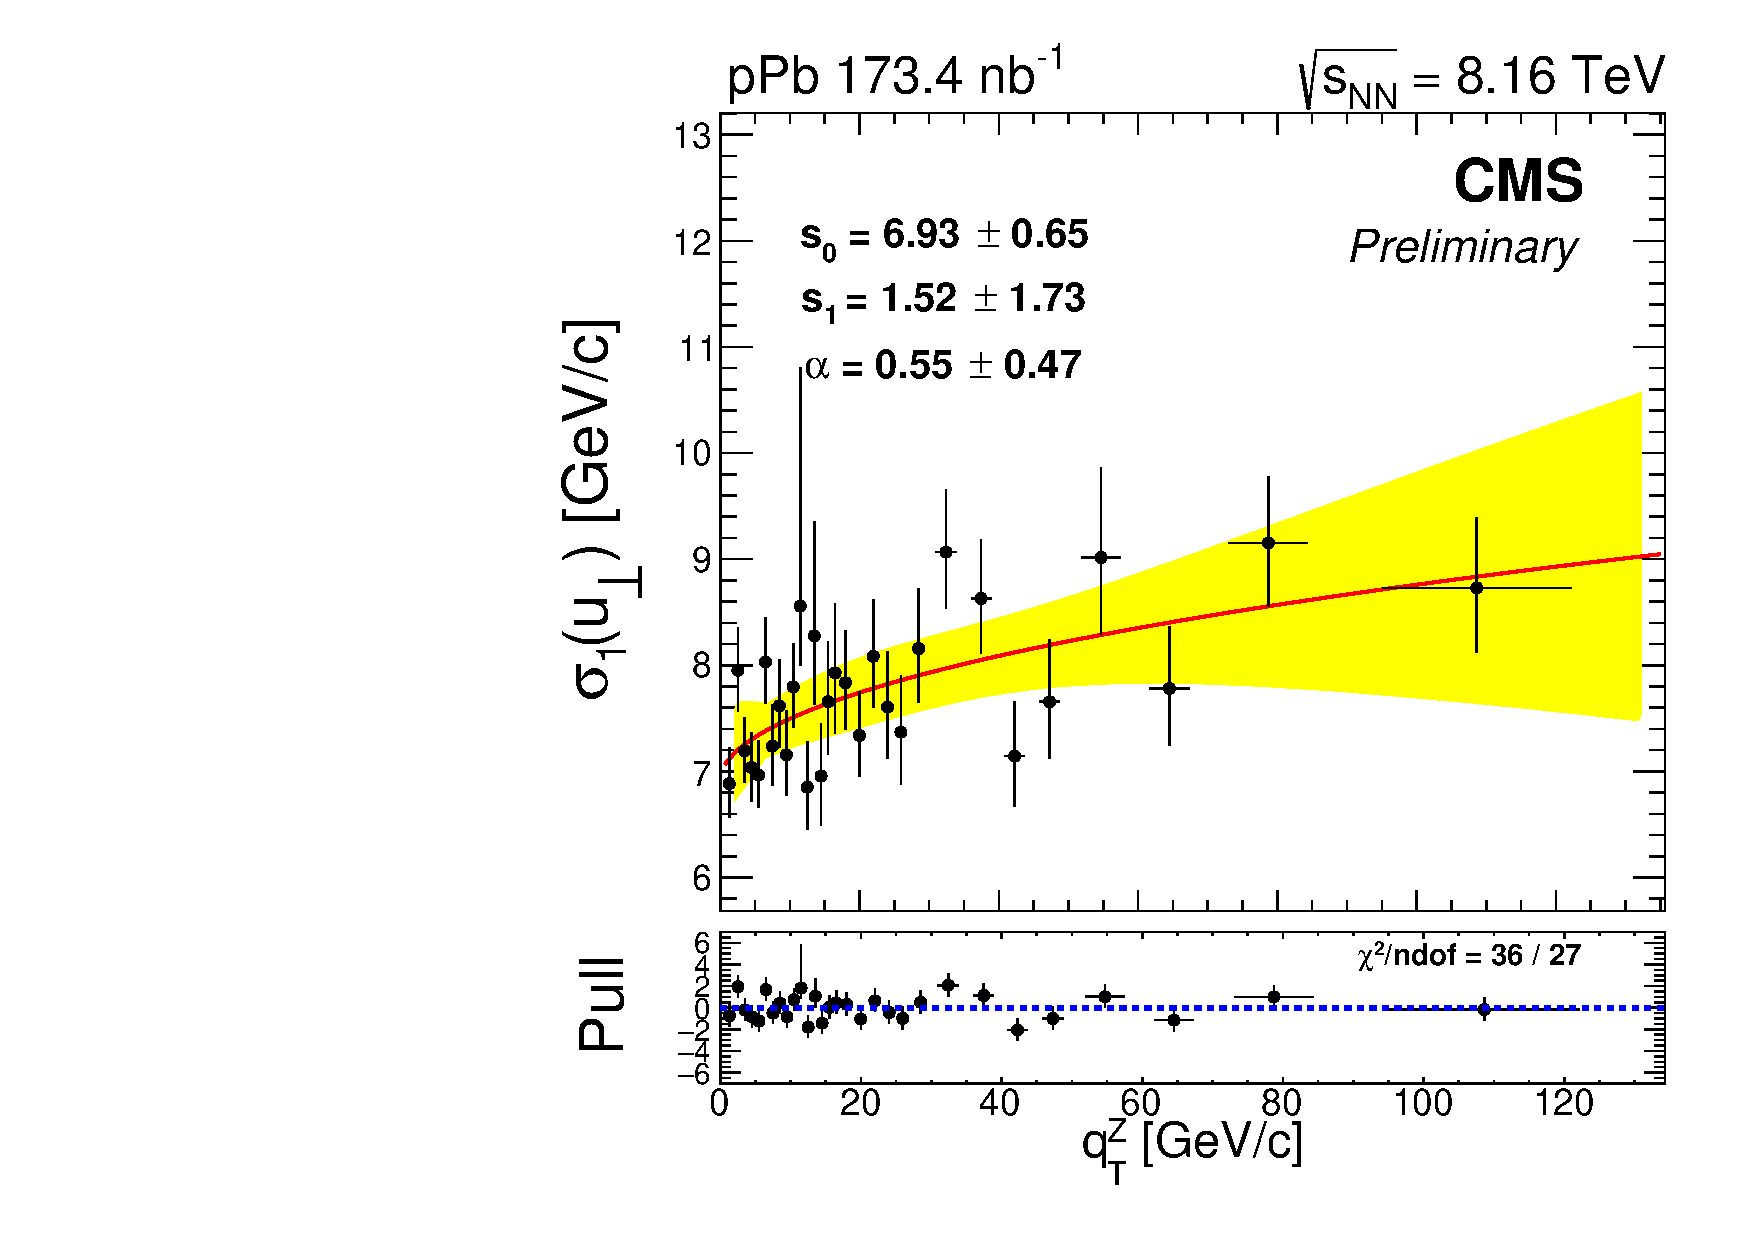
\includegraphics[width=0.3\textwidth]{Figures/WBoson/Analysis/Correction/Recoil/RecoilFitsqT/Data/fitPFu2sigma1.pdf}
 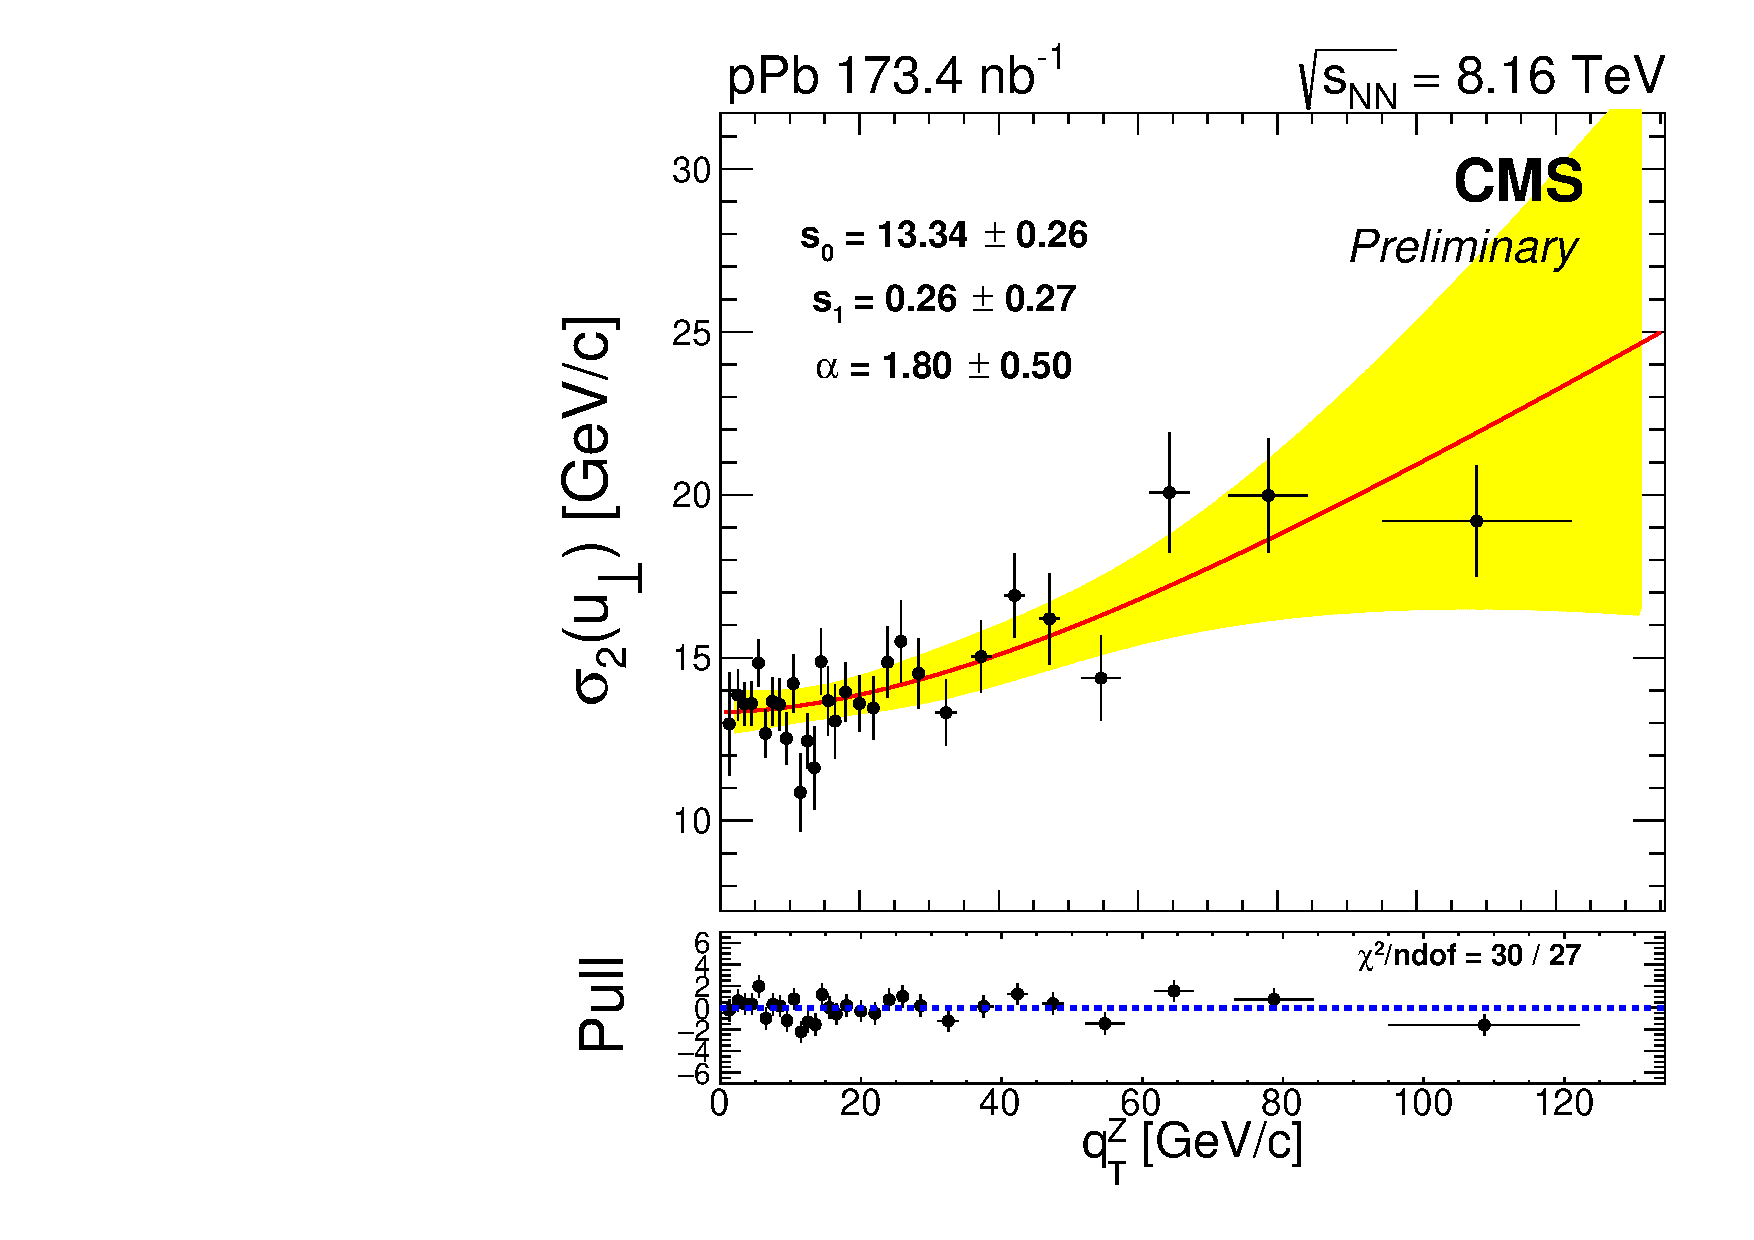
\includegraphics[width=0.3\textwidth]{Figures/WBoson/Analysis/Correction/Recoil/RecoilFitsqT/Data/fitPFu2sigma2.pdf}
 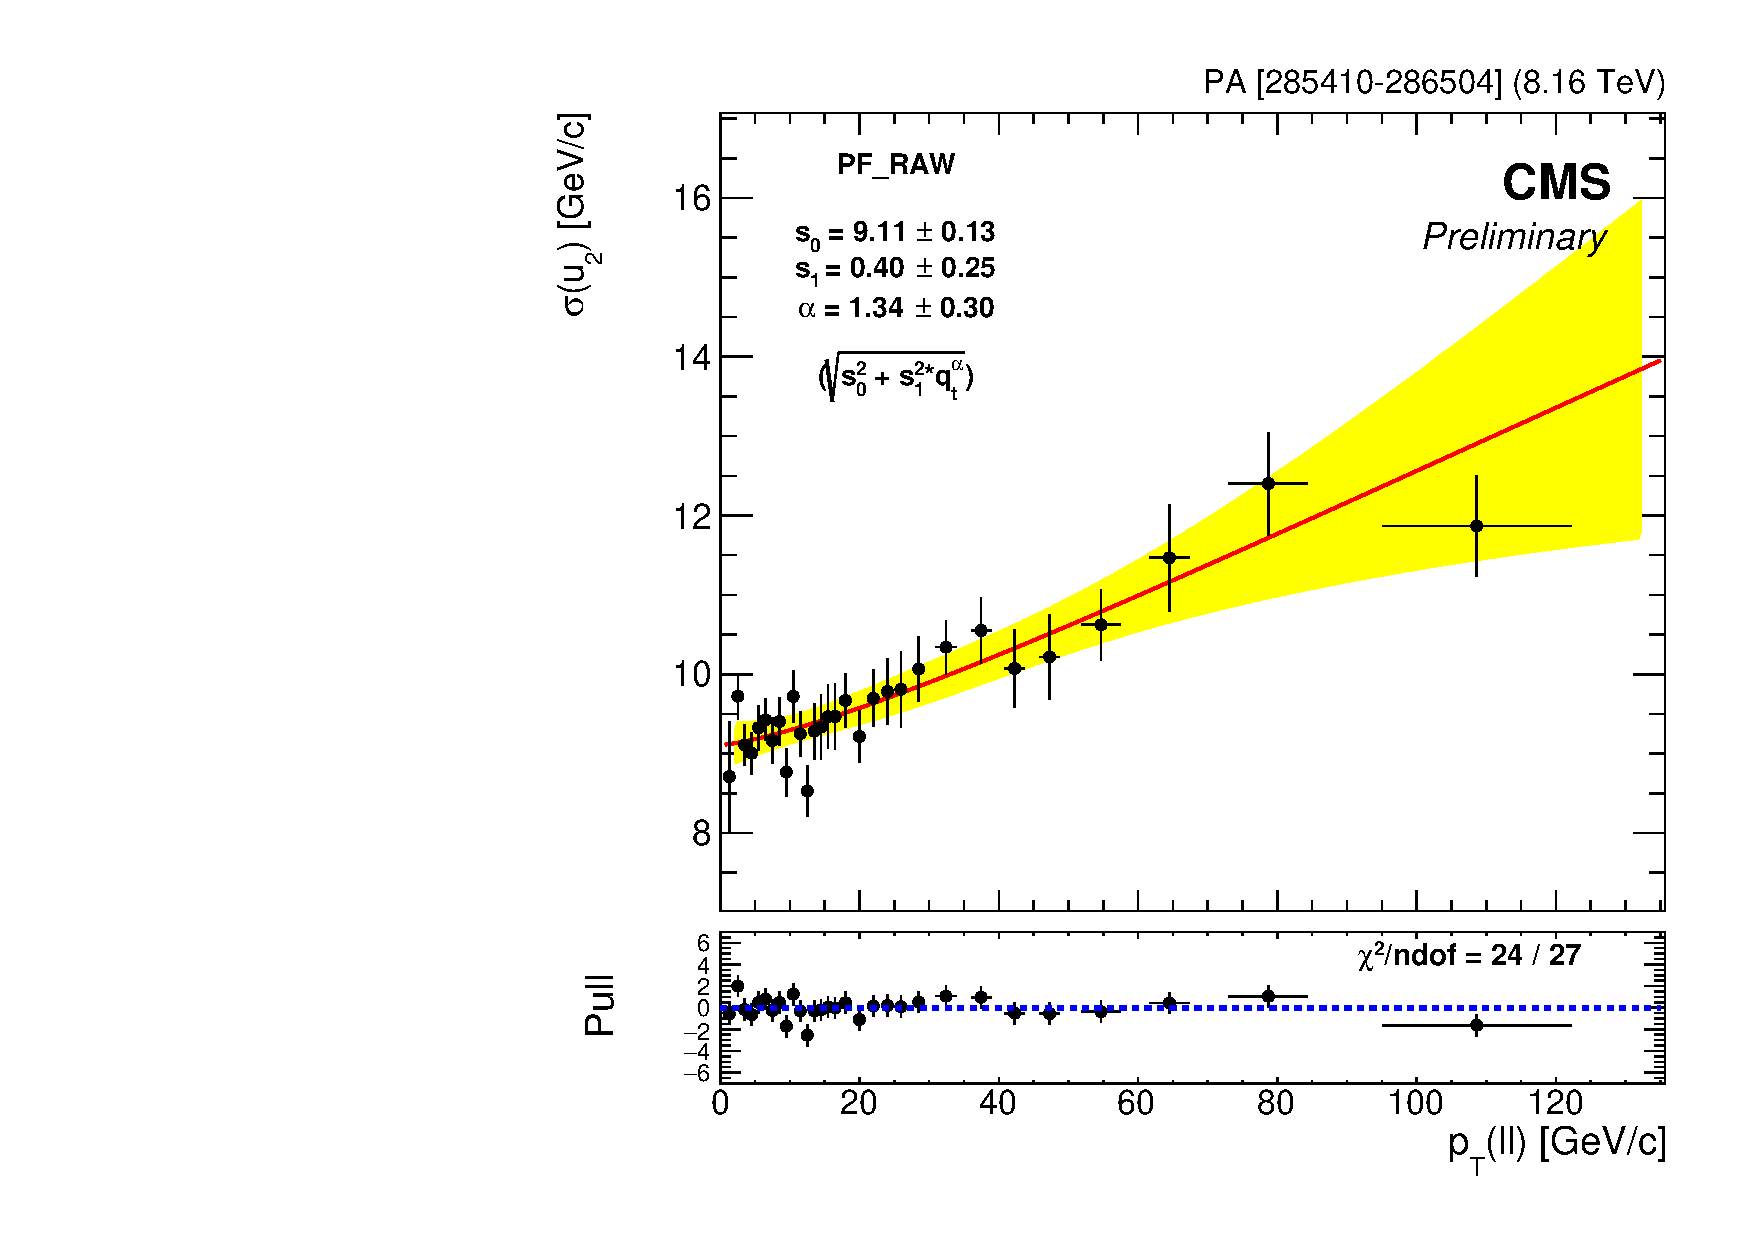
\includegraphics[width=0.3\textwidth]{Figures/WBoson/Analysis/Correction/Recoil/RecoilFitsqT/Data/fitPFu2sigma.pdf} \\
 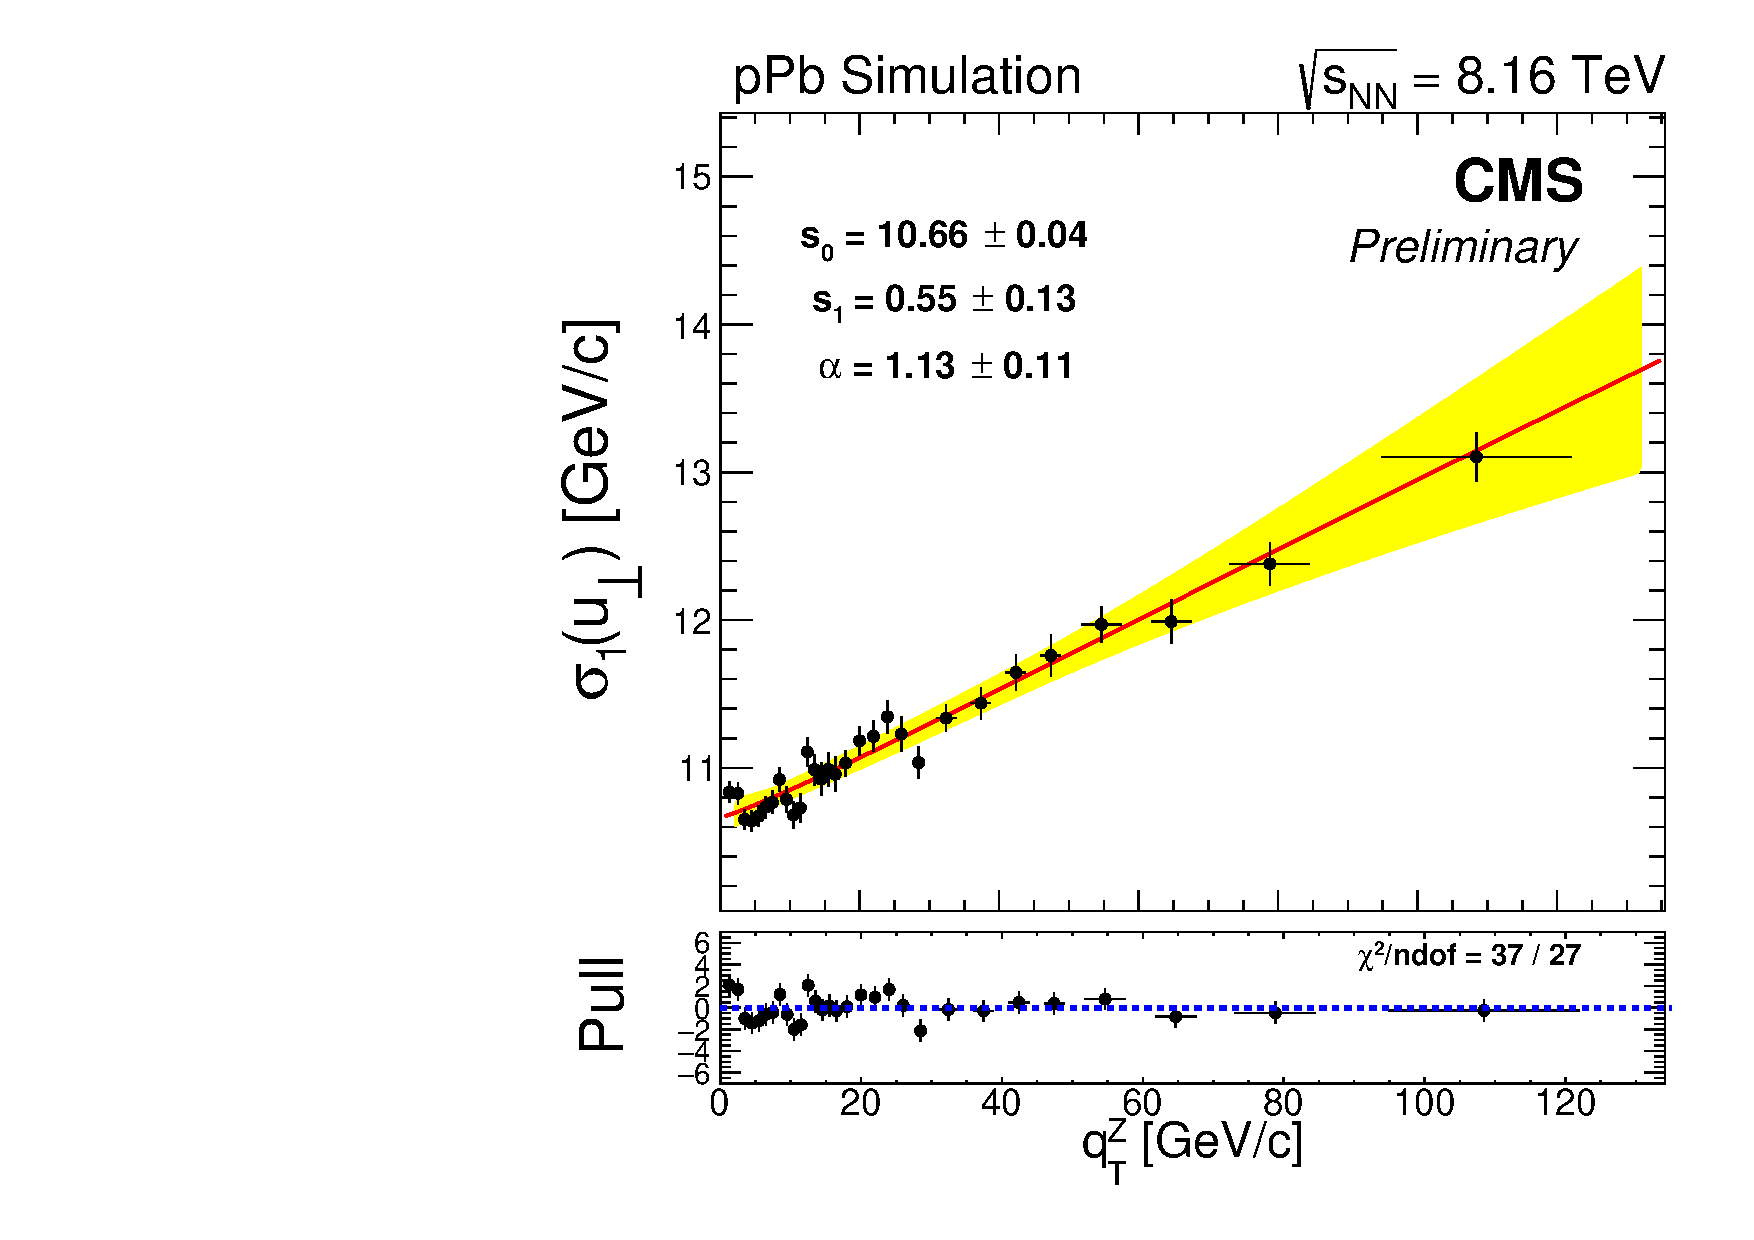
\includegraphics[width=0.3\textwidth]{Figures/WBoson/Analysis/Correction/Recoil/RecoilFitsqT/MC/fitPFu2sigma1.pdf}
 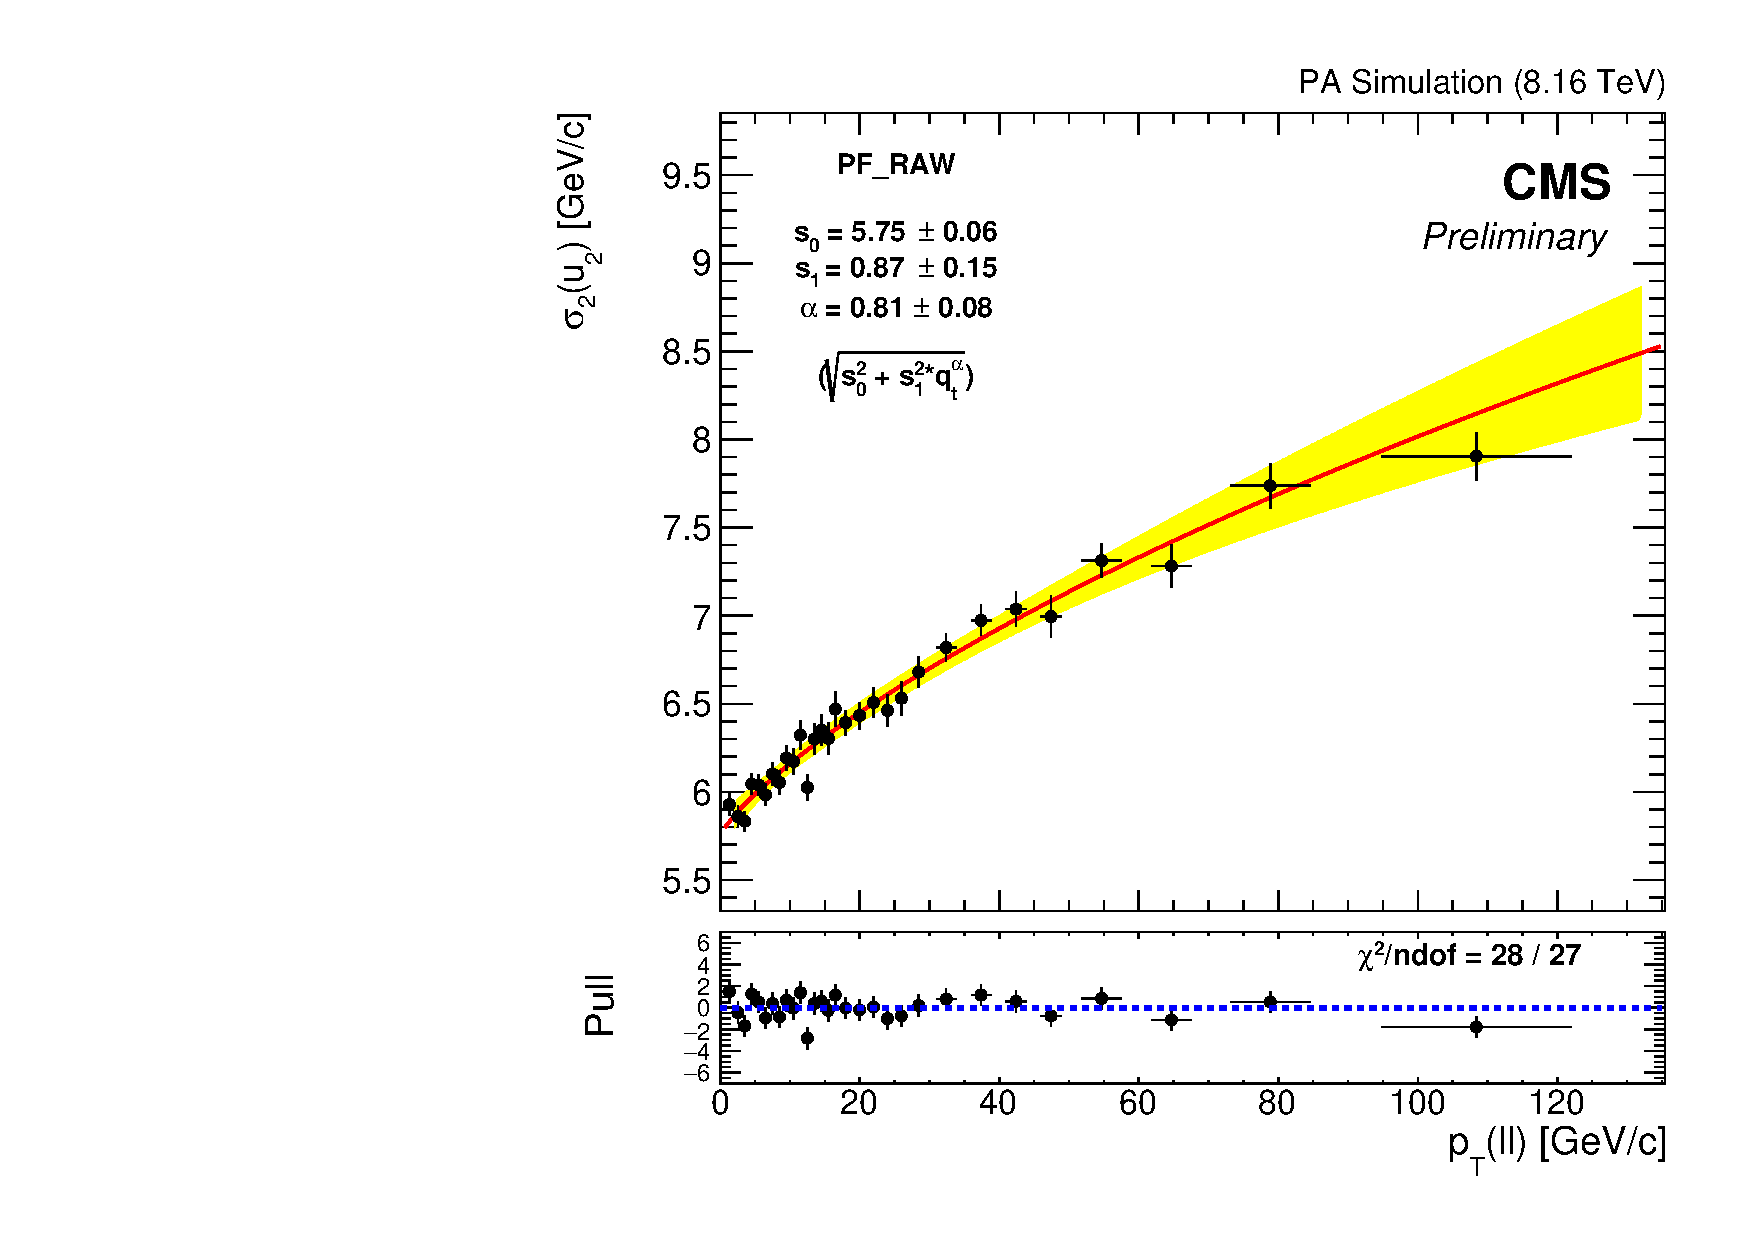
\includegraphics[width=0.3\textwidth]{Figures/WBoson/Analysis/Correction/Recoil/RecoilFitsqT/MC/fitPFu2sigma2.pdf}
 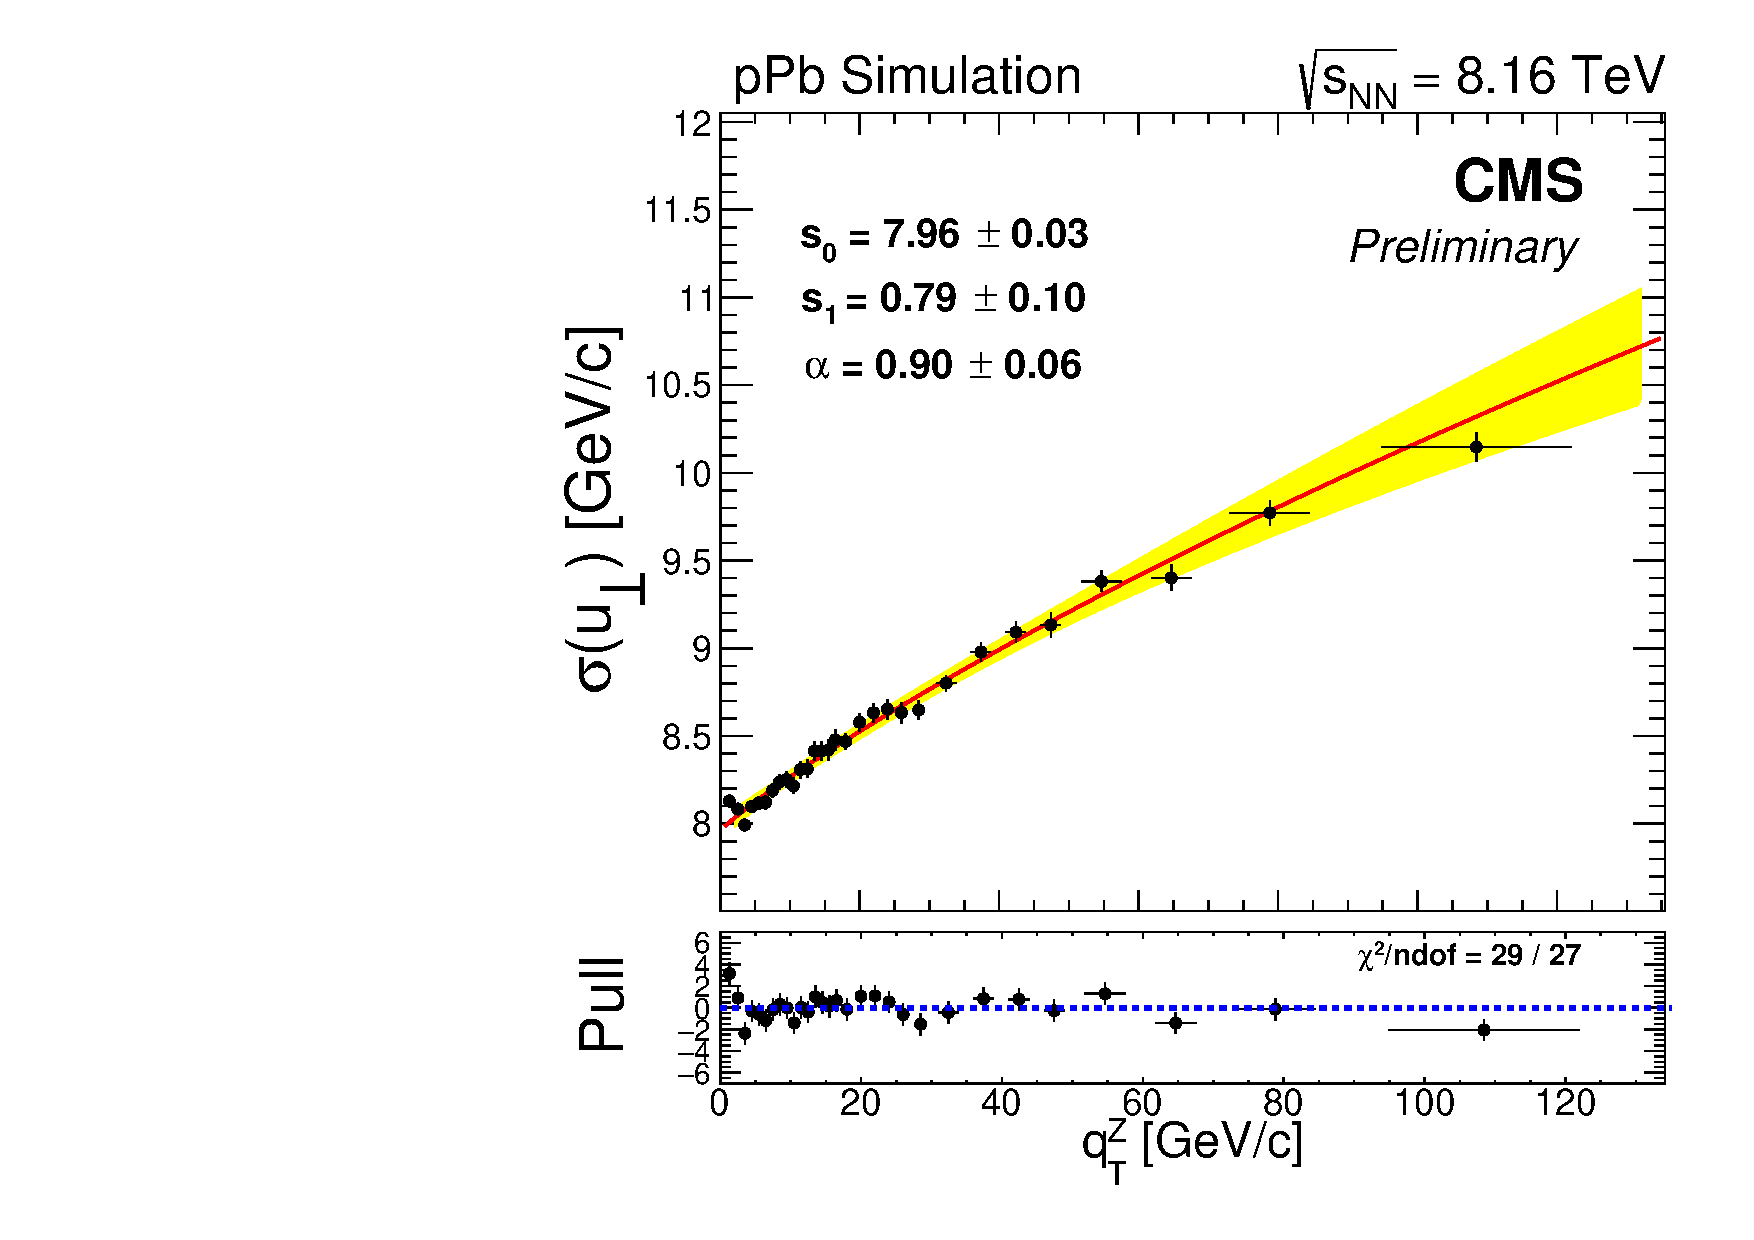
\includegraphics[width=0.3\textwidth]{Figures/WBoson/Analysis/Correction/Recoil/RecoilFitsqT/MC/fitPFu2sigma.pdf}
 \caption{Fits for the $\sigma_{\perp,1}$ (left), $\sigma_{\perp,2}$ (middle) and weighed average $\sigma_{\perp}$ (right) values of the recoil perpendicular component as a function of $q_{T}$. The results are derived from \ZToMuMu events in data (top) and simulation (bottom).}
 \label{fig:figU2RecoilResolutionFit}
\end{figure}

It is observed in \fig{fig:figU1RecoilResolutionFit} and \ref{fig:figU2RecoilResolutionFit}, that the recoil resolution increases with \qtZ. This is expected since high-\pt \Z bosons are produced in association with several jets from higher order processes, which contributes to the recoil resolution. 

Also, the parameter $s_{0}$ of the weighed average $\sigma$, which measure the recoil resolution at $\qtZ = 0~\GeVc$, is found to be larger in data than in simulation, which means that the modelling of the contributions not originating from the hard scattering (e.g. underlying events) are underestimated compared to data. In addition, the contributions to the recoil resolution at high \qtZ are also larger in data than in simulation.

\paragraph{Calibration of the simulated recoil.} The recoil corrections are applied to the following simulated processes: \WToMuNu, \DYToMuMu and \WToTauNu. The simulated recoil distribution is calibrated using the parametric equations obtained in the previous sections for the Gaussian mean $\mu(\qt)$ and weighed-average  width $\sigma(\qt)$. These parametric equations are summarised below:
\begin{itemize}
  \item Recoil parametric equations from data: 
\begin{equation}
 \begin{aligned}
  \mu^{\text{data}}_{\parallel}\left(\qt\right) &= \left(0.5 + 0.9{\cdot}\qt\right)\left(\frac{1 + \text{Erf}\left[0.1{\cdot}\left(\qt\right)^{0.7}\right]}{2}\right) \\
  \sigma^{\text{data}}_{\parallel}\left(\qt\right) &= \sqrt{9.1^{2} + 0.4^{2}{\cdot}\left(\qt\right)^{1.5}} \\
  \sigma^{\text{data}}_{\perp}\left(\qt\right) &= \sqrt{9.1^{2} + 0.4^{2}{\cdot}\left(\qt\right)^{1.3}}
 \end{aligned}
\end{equation}
  \item Recoil parametric equations from simulation:
\begin{equation}
 \begin{aligned}
  \mu^{\text{MC}}_{\parallel}\left(\qt\right) &= \left(0.1 + 0.9{\cdot}\qt\right)\left(\frac{1 + \text{Erf}\left[0.2{\cdot}\left(\qt\right)^{0.5}\right]}{2}\right) \\
  \sigma^{\text{MC}}_{\parallel}\left(\qt\right) &= \sqrt{8.1^{2} + 0.5^{2}{\cdot}\left(\qt\right)^{1.4}} \\
  \sigma^{\text{MC}}_{\perp}\left(\qt\right) &= \sqrt{8.0^{2} + 0.8^{2}{\cdot}\left(\qt\right)^{0.9}}
 \end{aligned}
\end{equation}
\end{itemize}

The procedure to calibrate the simulated recoil starts by computing the \pt vector of the boson (\qtvec) and simulated recoil ($\utvec^{\text{MC}}$). The boson \qtvec is determined using the reconstructed muon information whenever possible, as described below:
\begin{itemize}
 \item \WToMuNu: \qtvec is the \ptvec sum of the reconstructed muon and generated neutrino.
 \item \WToTauNu: \qtvec is the generated \Wb boson \pt vector.
 \item \DYToMuMu: if one of the muons is not reconstructed, then \qtvec is the \ptvec sum of the reconstructed  muon and the generated-only muon, otherwise \qtvec is equal to the \ptvec sum of both reconstructed muons ($\qtvec^{\DY}$).
\end{itemize}

The recoil $\utvec^{\text{MC}}$ of the simulated event is derived by \textit{removing} from the \ptvecmiss, the reconstructed muons from the decay of the weak boson. In other words, for \WToMuNu events, $\DYToMuMu$ events with only one reconstructed muon ($\DY\to\mu$) and \WToTauNu events, the $\utvec^{\text{MC}} = -\ptvecmiss - \ptMuvec$, while for \DYToMuMu events with both muons reconstructed, the $\utvec^{\text{MC}} = -\ptvecmiss - \qtvec^{\DY}$.

Once the $\utvec^{\text{MC}}$ and \qtvec have been derived for a given event, the $\utvec^{\text{MC}}$ is then separated in a component parallel ($\utpar^{\text{MC}}$) and perpendicular ($\utper^{\text{MC}}$) to the direction of \qtvec. The simulated recoil components are then scaled event-by-event, according to:

\begin{equation}
 \begin{aligned}
  \utpar^{\corr} &= \left(\utpar^{\text{MC}} - \mu_{\parallel}^{\text{MC}}\left(\qt\right)\right){\cdot}\left(\frac{\sigma_{\parallel}^{\text{data}}\left(\qt\right)}{\sigma_{\parallel}^{\text{MC}}\left(\qt\right)}\right) + \mu_{\parallel}^{\text{data}}\left(\qt\right) \\
  \utper^{\corr} &= \utper^{\text{MC}}{\cdot}\left(\frac{\mu_{\perp}^{\text{data}}\left(\qt\right)}{\sigma_{\perp}^{\text{MC}}\left(\qt\right)}\right)
 \end{aligned}
 \label{eq:RecoilCorr}
\end{equation}

Afterwards, the corrected recoil $\utvec^{\corr}$ is propagated to the \ptmiss of the event, as follows:

\begin{itemize}
 \item For \WToMuNu, \WToTauNu and $\DY\to\mu$ events:
\begin{equation}
 \ptmiss = \abs{\ut^{\corr} + \ptMuvec}
\end{equation}
 \item For fully reconstructed \DYToMuMu events:
\begin{equation}
 \ptmiss = \abs{\ut^{\corr} + \qtvec^{\DY}}
\end{equation}
\end{itemize}


As an alternative method used to determine the systematic uncertainty associated to the recoil calibration method, the simulated recoil components are smeared, instead of being scaled, by generating a random recoil component per event according to the following Gaussian distribution functions:

\begin{equation}
 \begin{aligned}
  \utpar^{\corr} &= Gauss\left(\utpar - \mu_{\parallel}^{\text{MC}}\left(\qt\right) + \mu_{\parallel}^{\text{data}}\left(\qt\right), \sqrt{{\sigma_{\parallel}^{\text{data}}\left(\qt\right)}^{2} - {\sigma_{\parallel}^{\text{MC}}\left(\qt\right)}^{2}}\right) \\
  \utper^{\corr} &= Gauss\left(\utper, \sqrt{{\sigma_{\perp}^{\text{data}}\left(\qt\right)}^{2} - {\sigma_{\perp}^{\text{MC}}\left(\qt\right)}^{2}}\right)
 \end{aligned}
 \label{eq:RecoilCorrAlt}
\end{equation}


\paragraph{Closure test.} The recoil calibration is checked using the \ZToMuMu control sample. The \ptmiss spectrum from data and the corrected one from simulation are shown in \fig{fig:recoilClosure}. As can be observed, the agreement between data and simulation is significantly improved after applying the recoil calibration using the scaling method.

\begin{figure}[htb!]
 \centering
 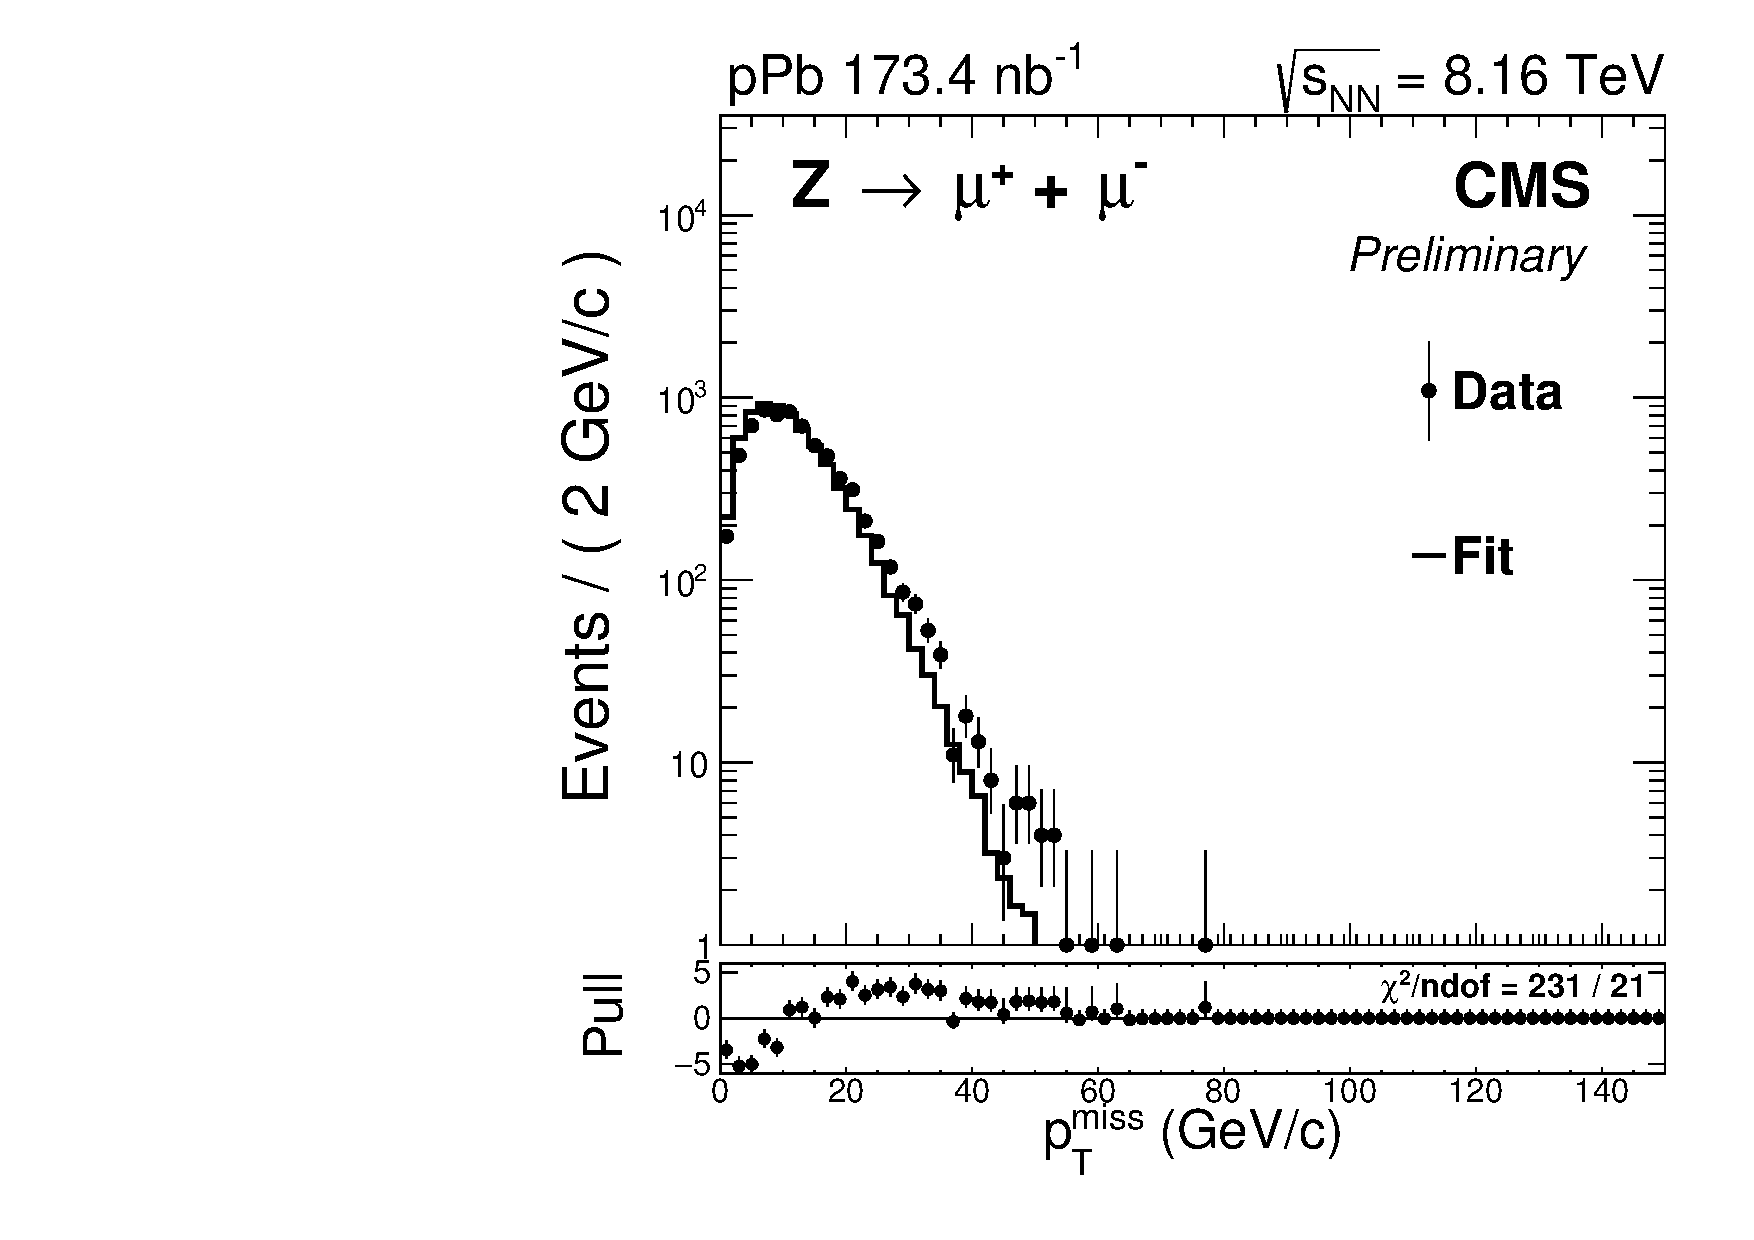
\includegraphics[width=0.45\textwidth]{Figures/WBoson/Analysis/Correction/Recoil/CheckFits/Z/METPF_RAW_HFBosonPTrew/PLOT_MET_DATA_ZToMuPl_PA_Model_TEMP_DY_MuEtaCM_-286_193_MuIso_0_15.pdf}
 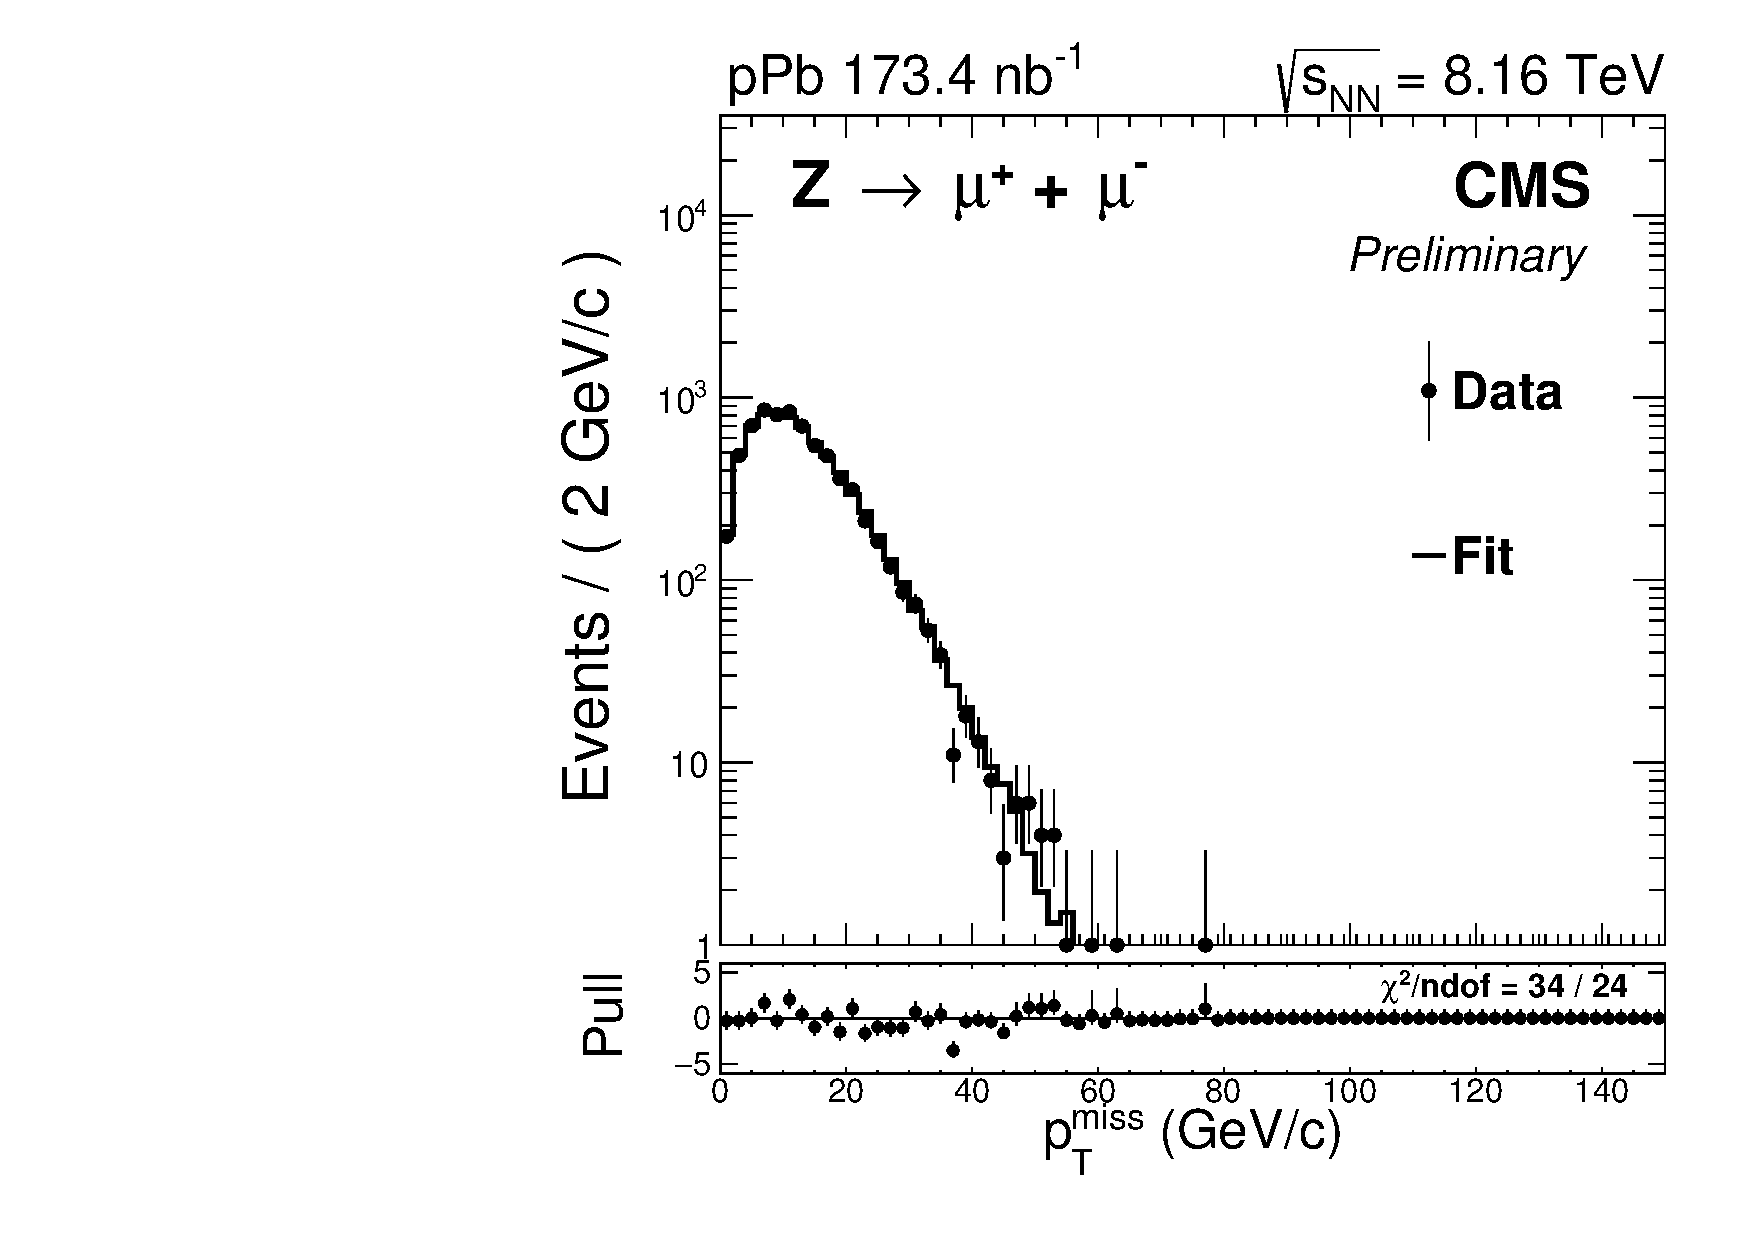
\includegraphics[width=0.45\textwidth]{Figures/WBoson/Analysis/Correction/Recoil/CheckFits/Z/Recoil_ScalingGauss/PLOT_MET_DATA_ZToMuPl_PA_Model_TEMP_DY_MuEtaCM_-286_193_MuIso_0_15.pdf}
 \caption{A comparison of the \ptmiss distribution from \ZToMuMu events between data and simulation, before (left) and after (right) calibrating the simulated recoil. The distributions of the simulated HF energy and generated \Z-boson \pt have been weighed.}
 \label{fig:recoilClosure}
\end{figure}


\paragraph{Impact of the recoil calibration in the signal region.} The \ptmiss distribution in the signal region is compared between data and the simulations. The fit to the data is performed following the signal extraction procedure described in \sect{sec:WBoson_Analysis_SignalExtraction}. The recoil corrections are applied to the electroweak simulations using both the nominal scaling method and the alternative smearing method, and the results are shown in \fig{fig:recoilCorrWreg}. Both the nominal and the alternative recoil calibrations improve significantly the agreement between the \ptmiss distribution extracted from data and simulations.

\begin{figure}[htb!]
 \centering
 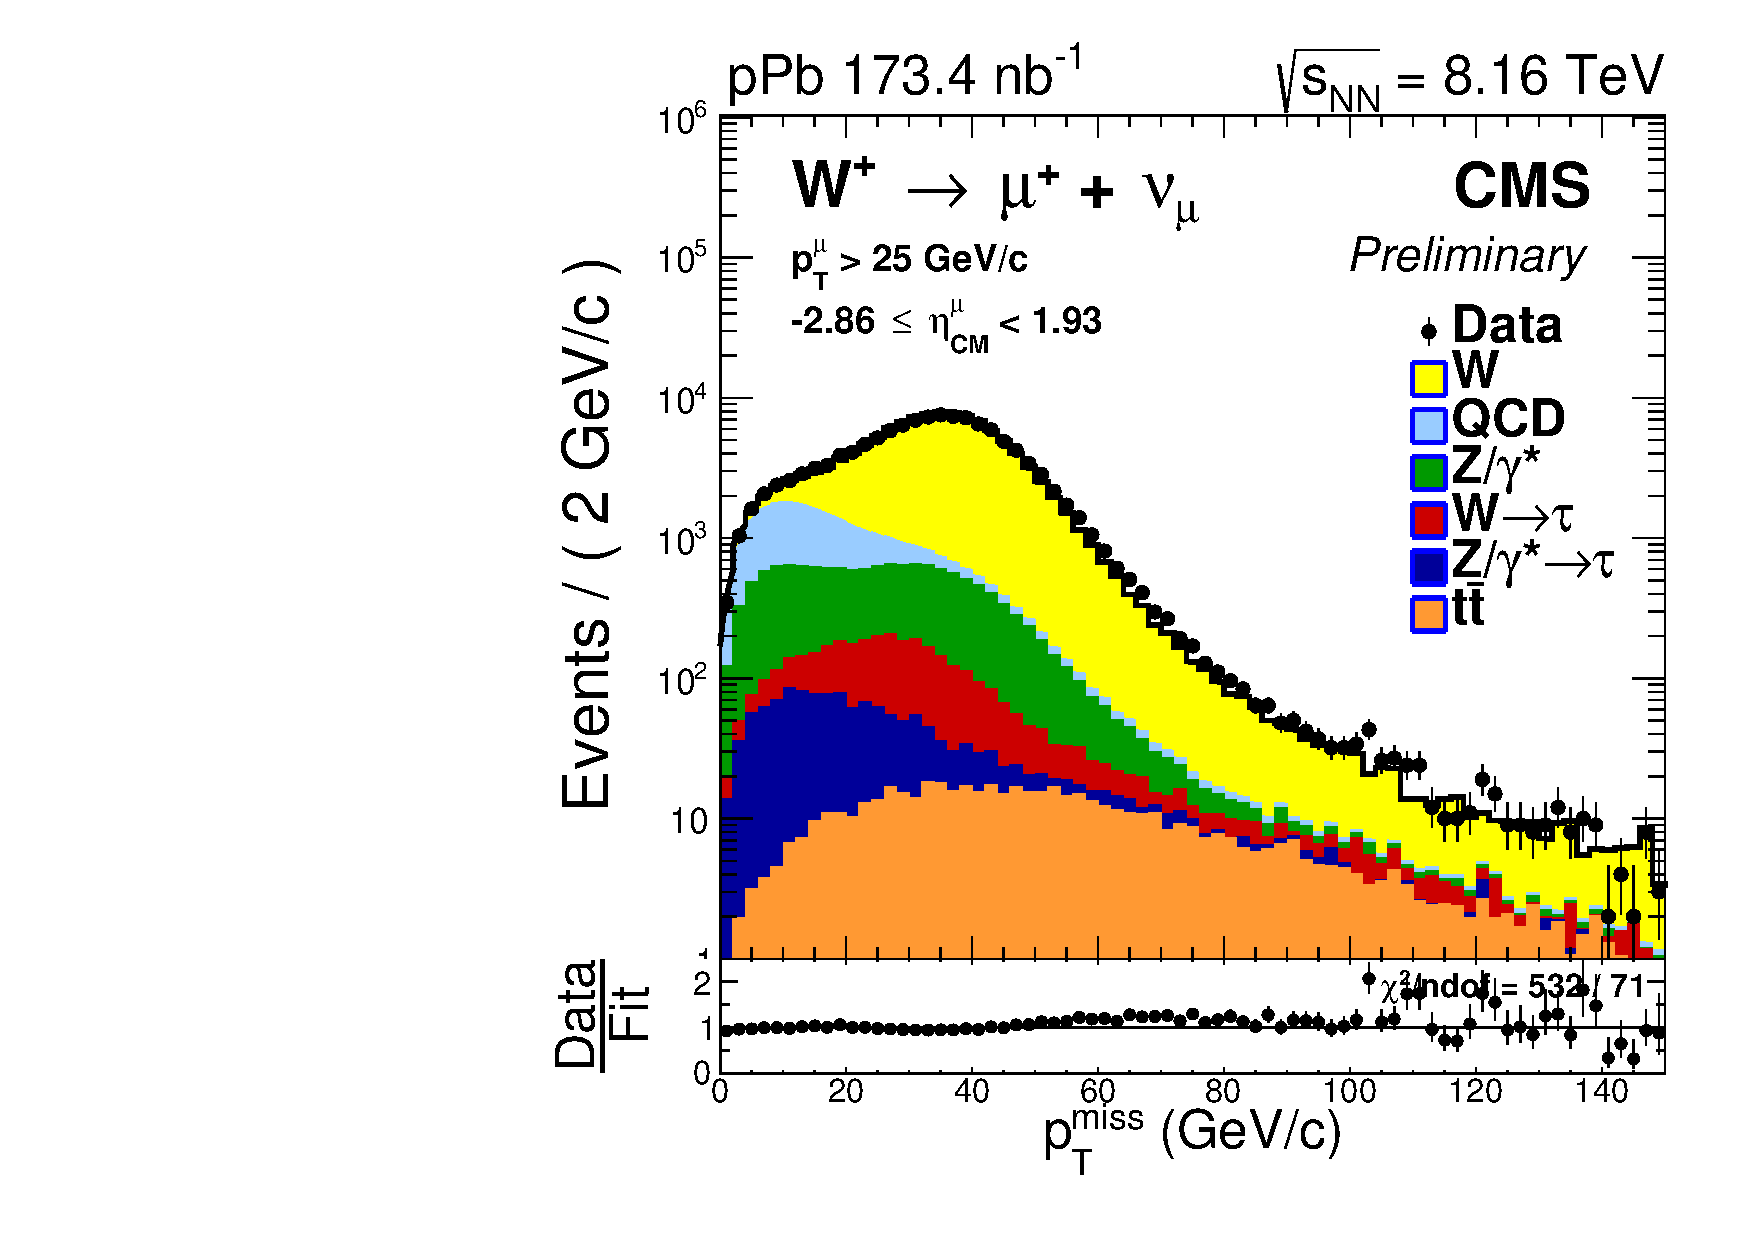
\includegraphics[width=0.45\textwidth]{Figures/WBoson/Analysis/Correction/Recoil/CheckFits/W/METPF_RAW_HFBosonPTrew/PLOT_MET_DATA_WToMuPl_PA_Model_TEMP_WDYDYToTauWToTauTTbar_ModifiedRayleigh_QCD_MuEtaCM_-286_193_MuIso_0_15.pdf}
 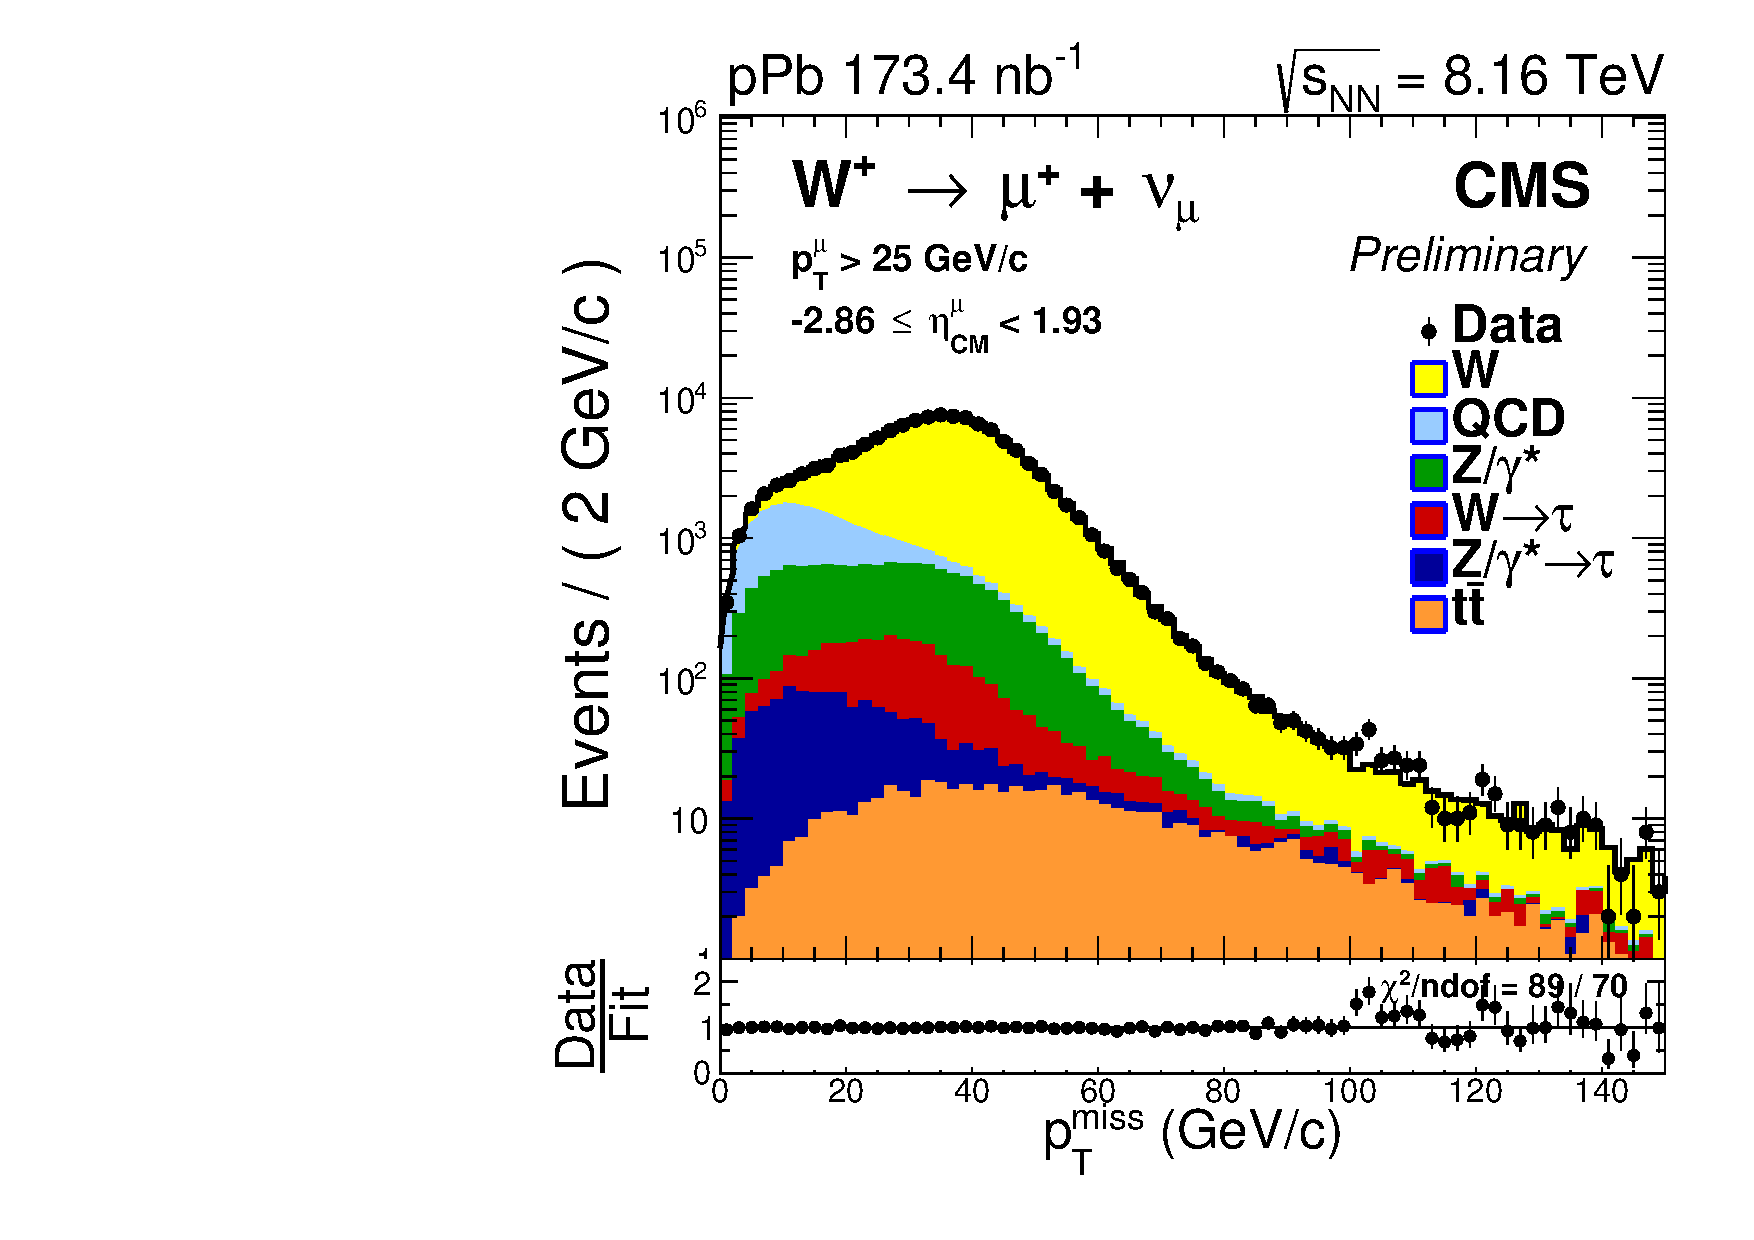
\includegraphics[width=0.45\textwidth]{Figures/WBoson/Analysis/Correction/Recoil/CheckFits/W/Recoil_ScalingGauss/PLOT_MET_DATA_WToMuPl_PA_Model_TEMP_WDYDYToTauWToTauTTbar_ModifiedRayleigh_QCD_MuEtaCM_-286_193_MuIso_0_15.pdf}
 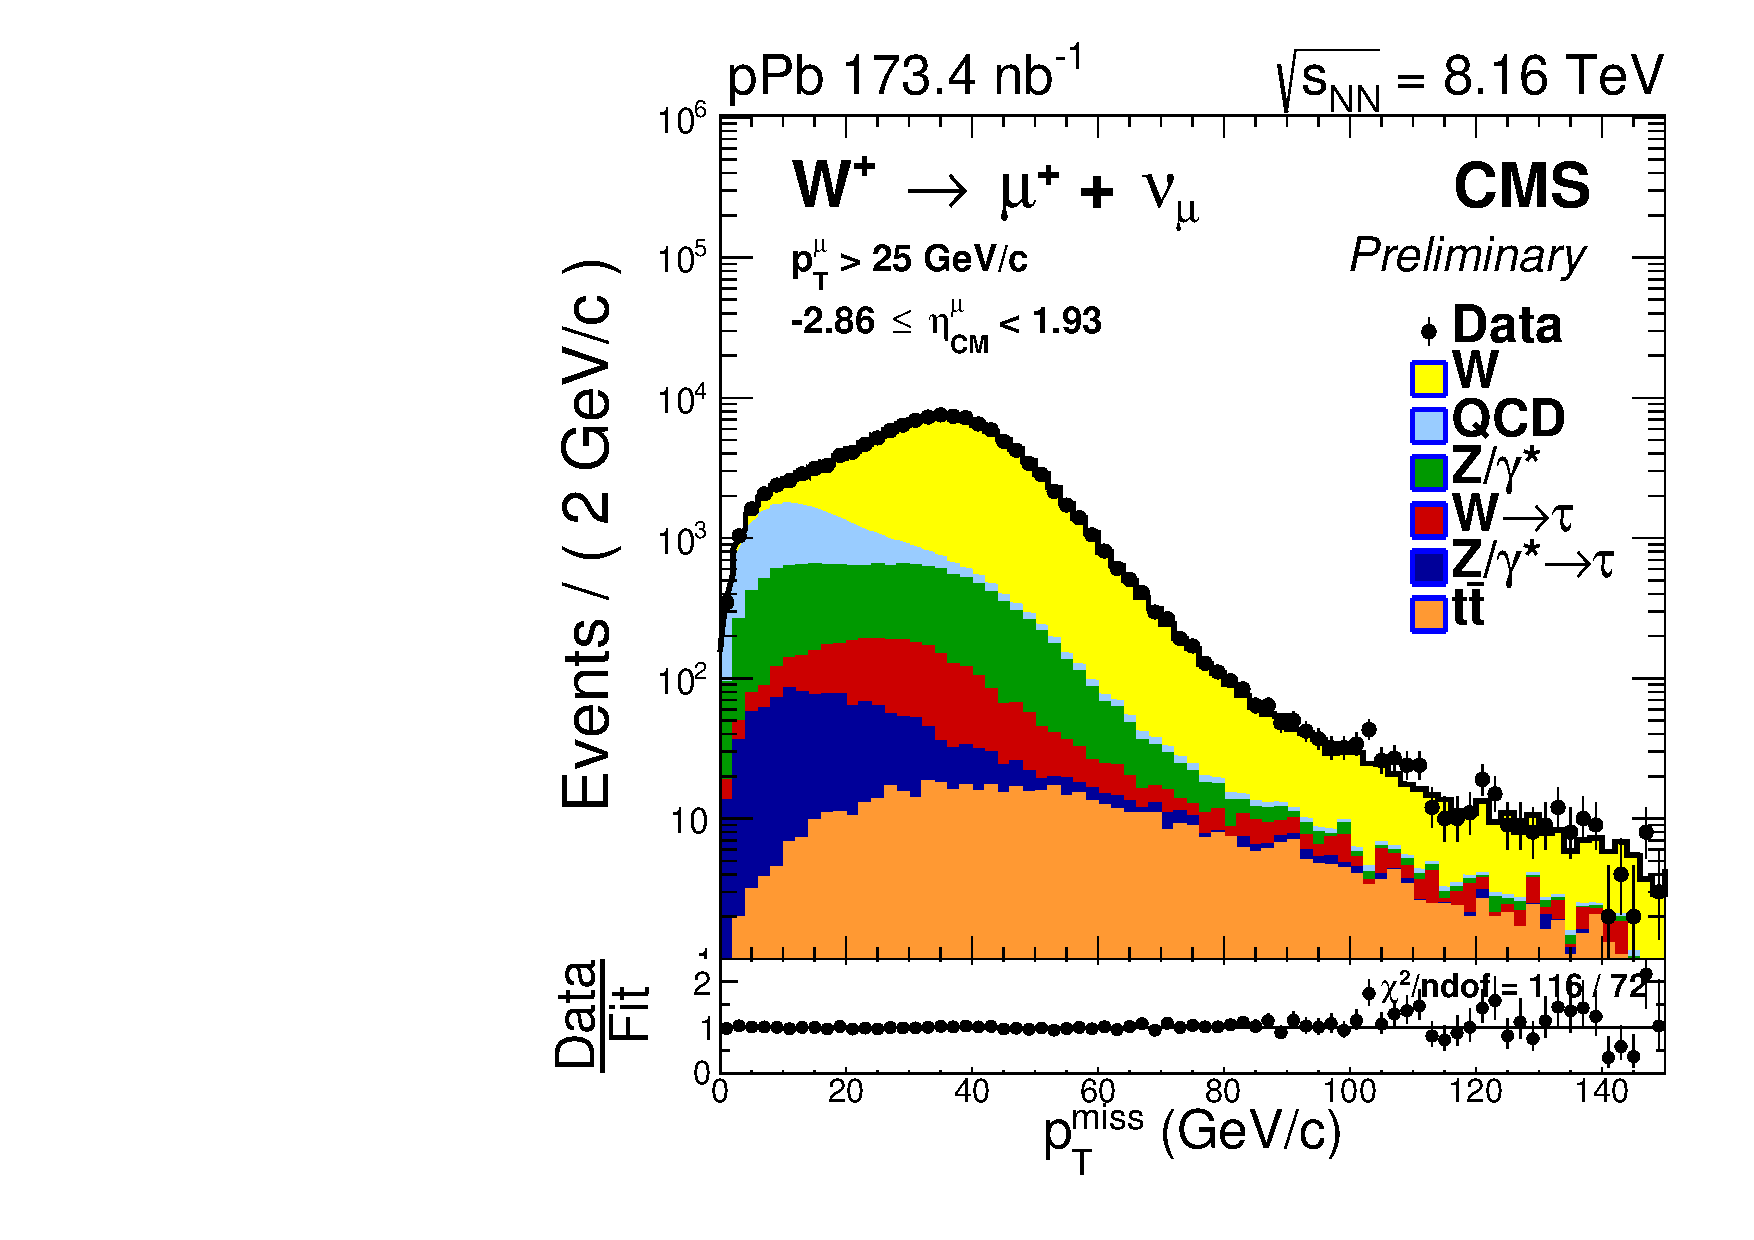
\includegraphics[width=0.45\textwidth]{Figures/WBoson/Analysis/Correction/Recoil/CheckFits/W/Recoil_Smearing/PLOT_MET_DATA_WToMuPl_PA_Model_TEMP_WDYDYToTauWToTauTTbar_ModifiedRayleigh_QCD_MuEtaCM_-286_193_MuIso_0_15.pdf}
 \caption{Comparison of the \ptmiss distribution in data and simulation for positive-charged muons in the  \etaMuCM-inclusive signal region. The results are shown before (top-left) and after (top-right) applying the recoil calibrations using the nominal scaling method. The result using the alternative smearing method (bottom) is also presented. The distributions of the simulated HF energy and generated \Z-boson \pt have been weighed.}
 \label{fig:recoilCorrWreg}
\end{figure}


% END OF SUBSECTION

\subsection{Signal efficiency}\label{sec:WBoson_Analysis_Efficiency}

The \WToMuNu signal efficiency is defined as the probability for a muon with $\pt > 25$~\GeVc and $\abs{\etaMuLAB} < 2.4$, to be reconstructed and pass all the analysis selection criteria. The signal efficiency is obtained from simulation as detailed in \sect{sec:WBoson_Analysis_Efficiency_Simulated} and then corrected using data-to-MC efficiency ratios derived with the tag-and-probe method as explained in \sect{sec:WBoson_Analysis_Efficiency_Corrected}.

\subsubsection{Simulated signal efficiency}\label{sec:WBoson_Analysis_Efficiency_Simulated}

The signal efficiency is estimated using the \WToMuNu simulations since they contain the full history of the signal events, including the generation and reconstruction of the particles. To improve the modelling of the event activity in \RunpPb and the \Wb-boson \pt spectrum, the distribution of the generated \Wb-boson \pt and  simulated HF energy is weighed per event as explained in \sect{sec:WBoson_Analysis_Corrections_WeakBosonPTReweighing} and \sect{sec:WBoson_Analysis_Corrections_EventActivityReweighing}, respectively.

A reconstructed muon is considered an offline muon if it satisfies the signal selection requirements. Among the selection criteria, an offline muon is required to satisfy the isolation and identification criteria defined in \sect{sec:WBoson_Analysis_Selection_MuonIdentification}, match the trigger, have $\ptMu~>~25$~\GeVc and be within the CMS detector coverage $|\etaMuLAB|~<~2.4$.

The signal efficiency of the simulated events is computed as the fraction of \textit{generated} muons matched to an \textit{offline} muon around a cone of $\Delta{R} = \sqrt{\Delta{\eta}^{2} + \Delta{\phi}^{2}} < 0.05$.  All generated muons are required to be within the analysis kinematic region ($\ptMu~>~25$~\GeVc and $\abs{\etaLAB}~<~2.4$) and come from a \Wb-boson decay. The signal efficiency of the \pPb and \Pbp \WToMuNu simulations is derived as a function of the generated muon \etaMuLAB, according to:

\begin{equation}
 \epsilon^{\mu^{\pm}}_{\pPb\,(\Pbp)}\left(\etaMuCM\right) = \left(\frac{N_{\text{off}}^{\mu^{\pm}}\left[\etaMuLAB\right]}{N_{\gen,\pt>25}^{\mu^{\pm}}\left[\etaMuLAB\right]}\right)_{\pPb\,(\Pbp)}
 \label{eq:MCTruthEfficiency}
\end{equation}

where $N_{\text{off}}$ and $N_{\gen}$ are the number of offline and generated muons, accordingly. A comparison of the signal efficiencies from the \pPb and \Pbp simulations is shown in \fig{fig:MCTruthComparison}. A good agreement between the two samples is observed.

\begin{figure}[htb!]
 \centering
 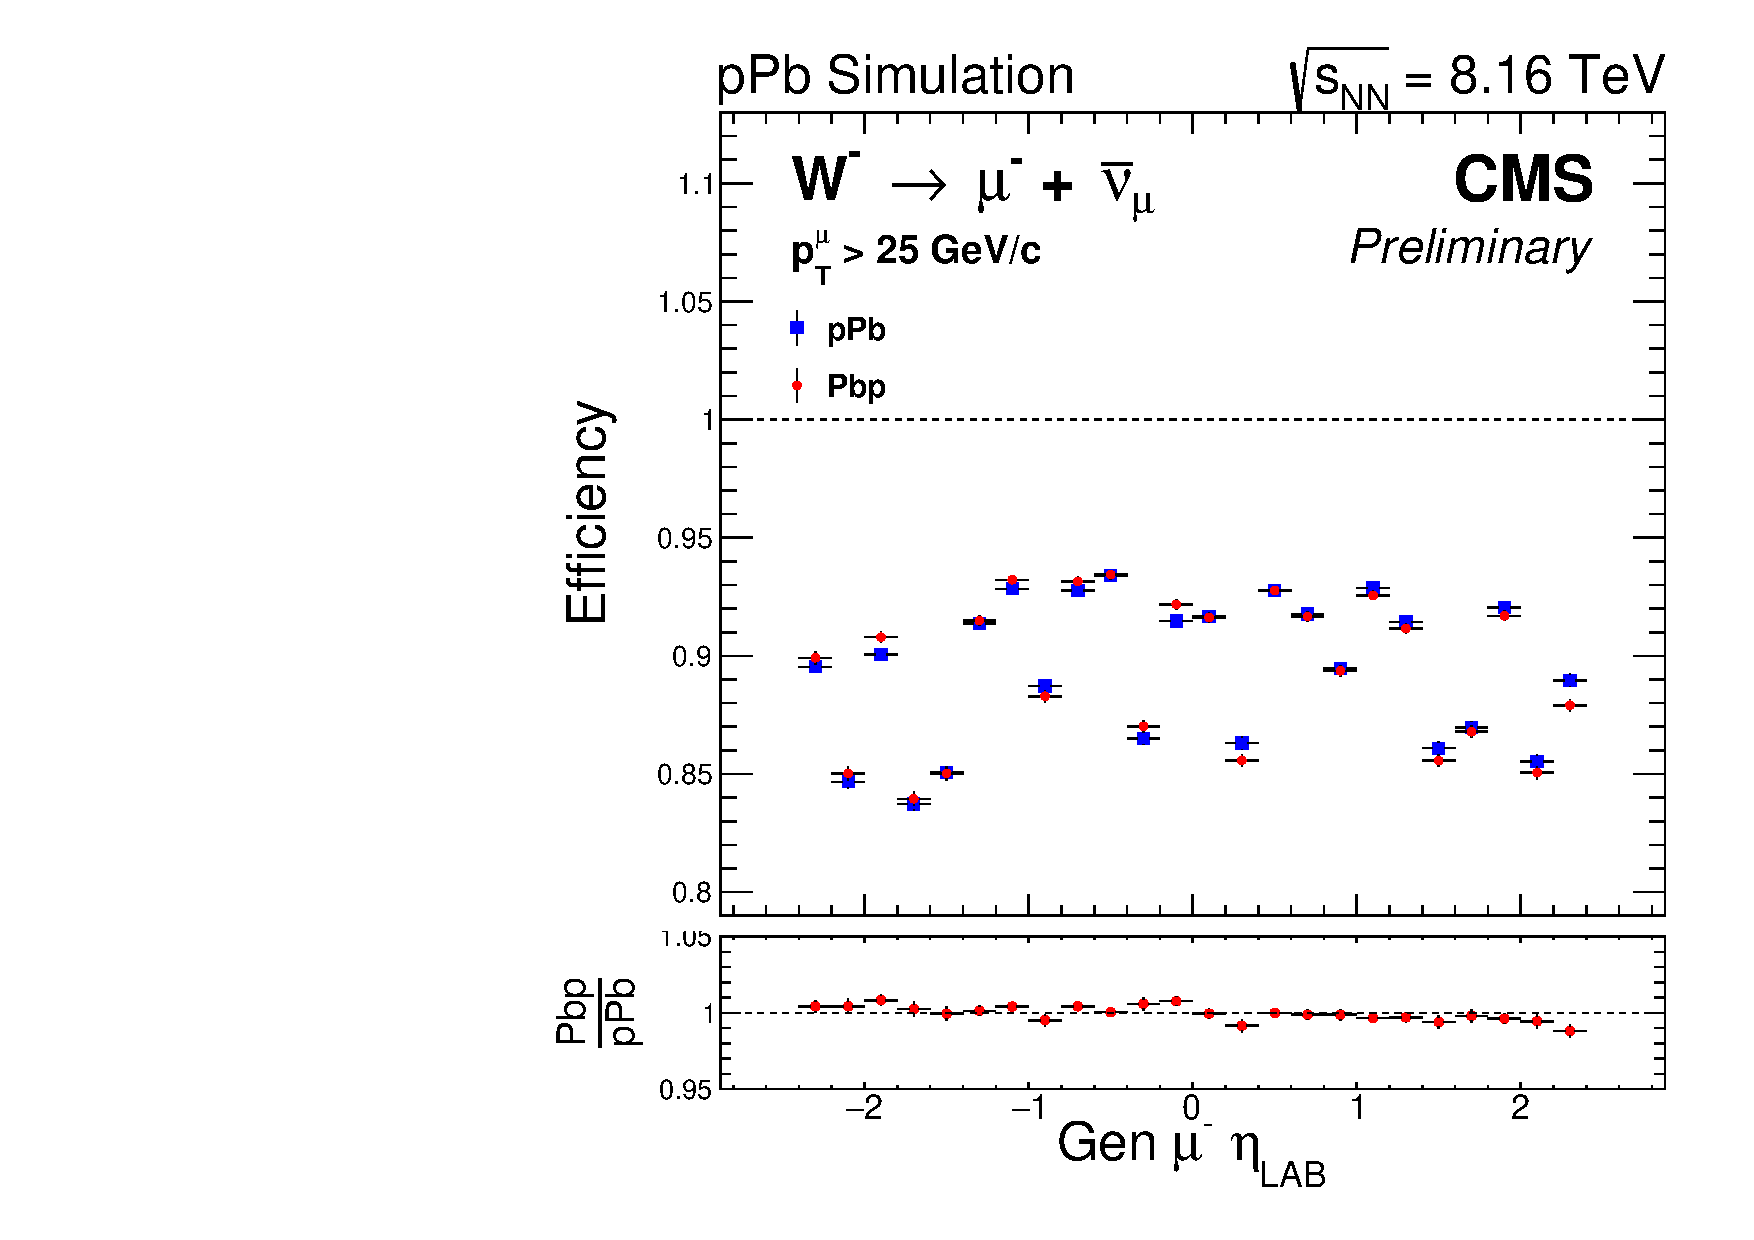
\includegraphics[width=0.45\textwidth]{Figures/WBoson/Analysis/Efficiency/eff1D_Eta_MC_WToMuNu_Minus_Total_HFCorr.pdf}
 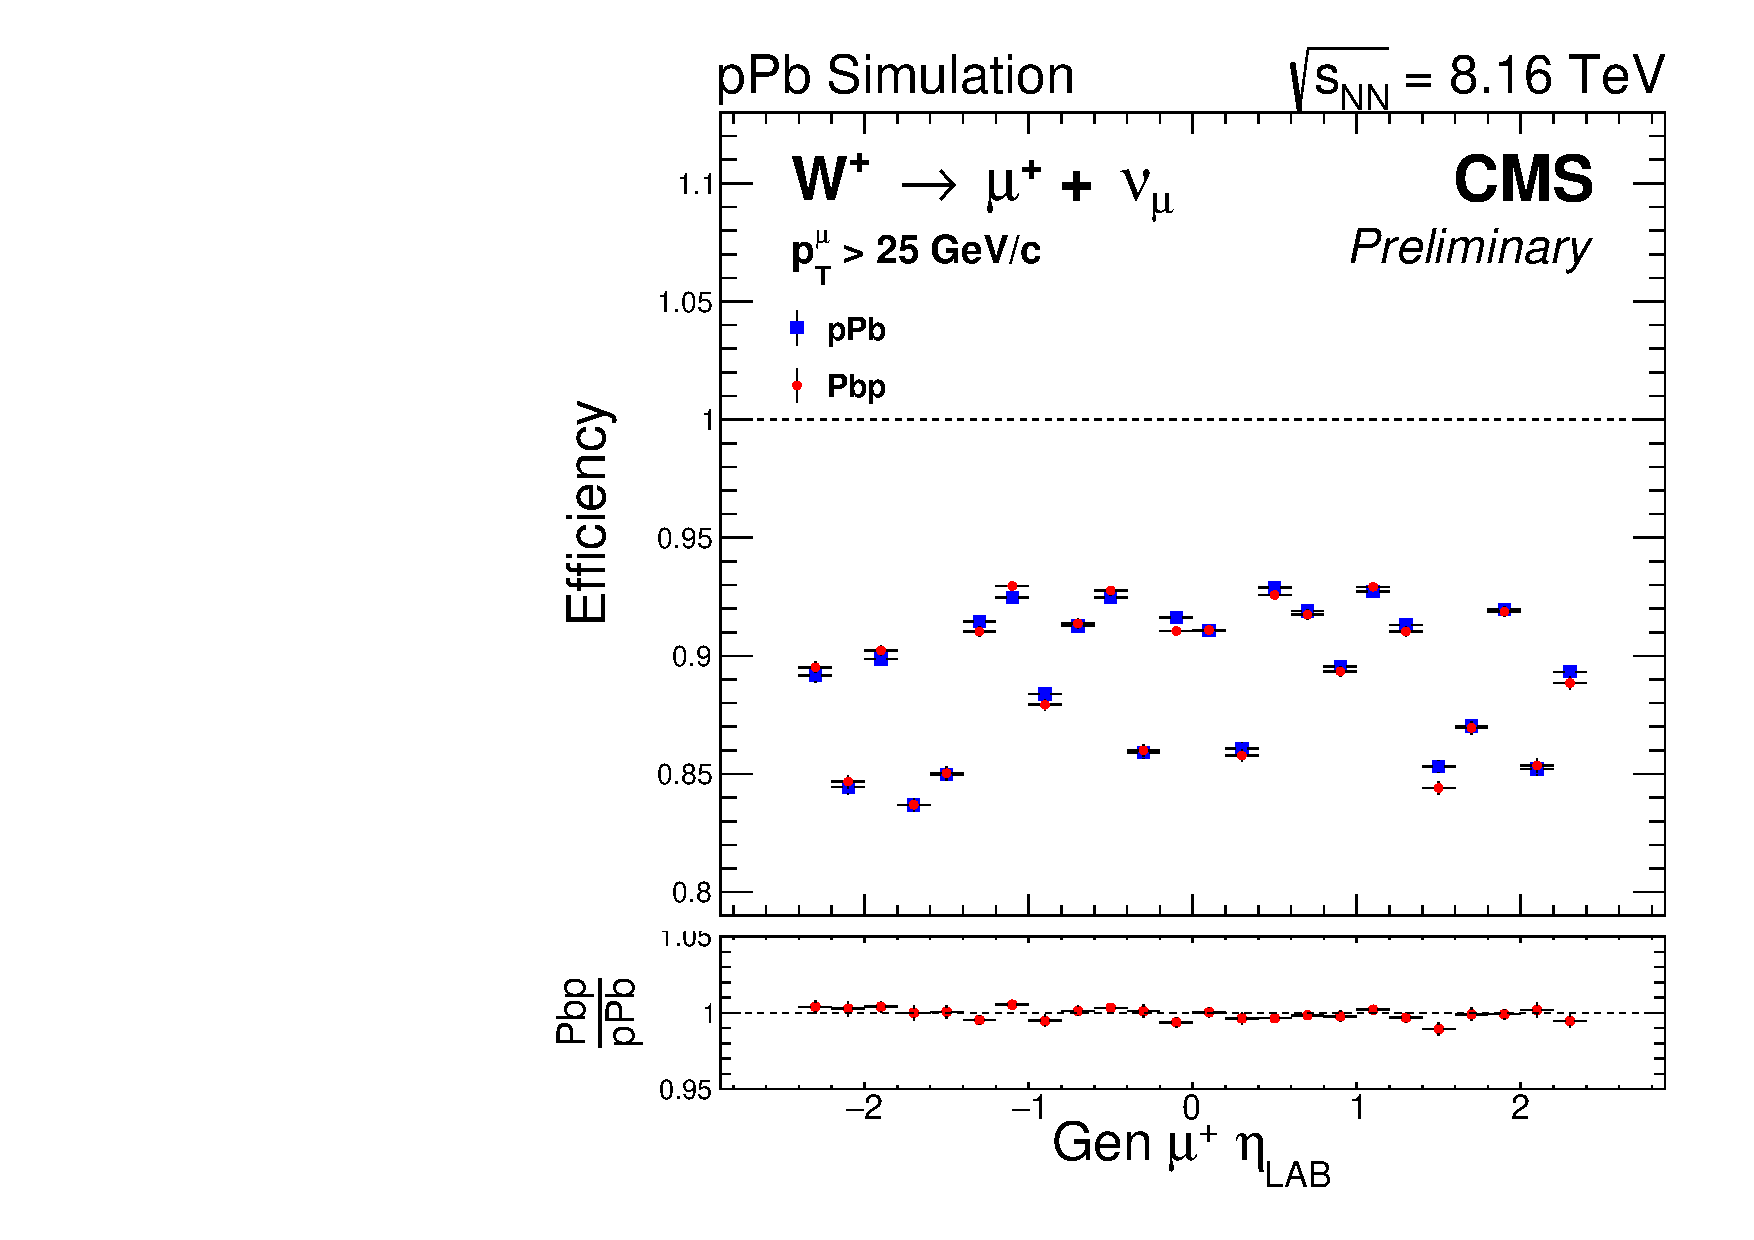
\includegraphics[width=0.45\textwidth]{Figures/WBoson/Analysis/Efficiency/eff1D_Eta_MC_WToMuNu_Plus_Total_HFCorr.pdf}
 \caption{Comparison of the signal efficiency derived from the \pPb and \Pbp \WToMuNu simulations as a function of the generated muon \etaLAB, separated in negative (left) and positive (right) charged muons. The distributions of the simulated HF energy and generated \Wb-boson \pt have been weighed. The bottom panel shows the ratio of \Pbp over \pPb signal efficiencies.}
 \label{fig:MCTruthComparison}
\end{figure}

The signal efficiencies extracted from the \pPb and \Pbp \WToMuNu simulations are then combined in the centre-of-mass frame, and the final simulated signal efficiency $\epsilon^{\mu^{\pm}}_{\MC}$ is obtained as:

\begin{equation}
 \epsilon^{\mu^{\pm}}_{\MC}\left(\etaMuCM\right) = \frac{\Lumi_{\pPb}\cdot\epsilon^{\mu^{\pm}}_{\pPb}\left(\etaMuCM\right) + \Lumi_{\Pbp}\cdot\epsilon^{\mu^{\pm}}_{\Pbp}\left(\etaMuCM\right)}{\Lumi_{\pPb} + \Lumi_{\Pbp}}
 \label{eq:MCEfficiencyPA}
\end{equation}

where $\Lumi_{\pPb}$ and $\Lumi_{\Pbp}$ are the recorded integrated luminosity of each \RunpPb run. The results of the \WToMuNu efficiency, extracted from the simulations, are shown in \fig{fig:MCTruthEfficiency}.

\begin{figure}[htb!]
 \centering
 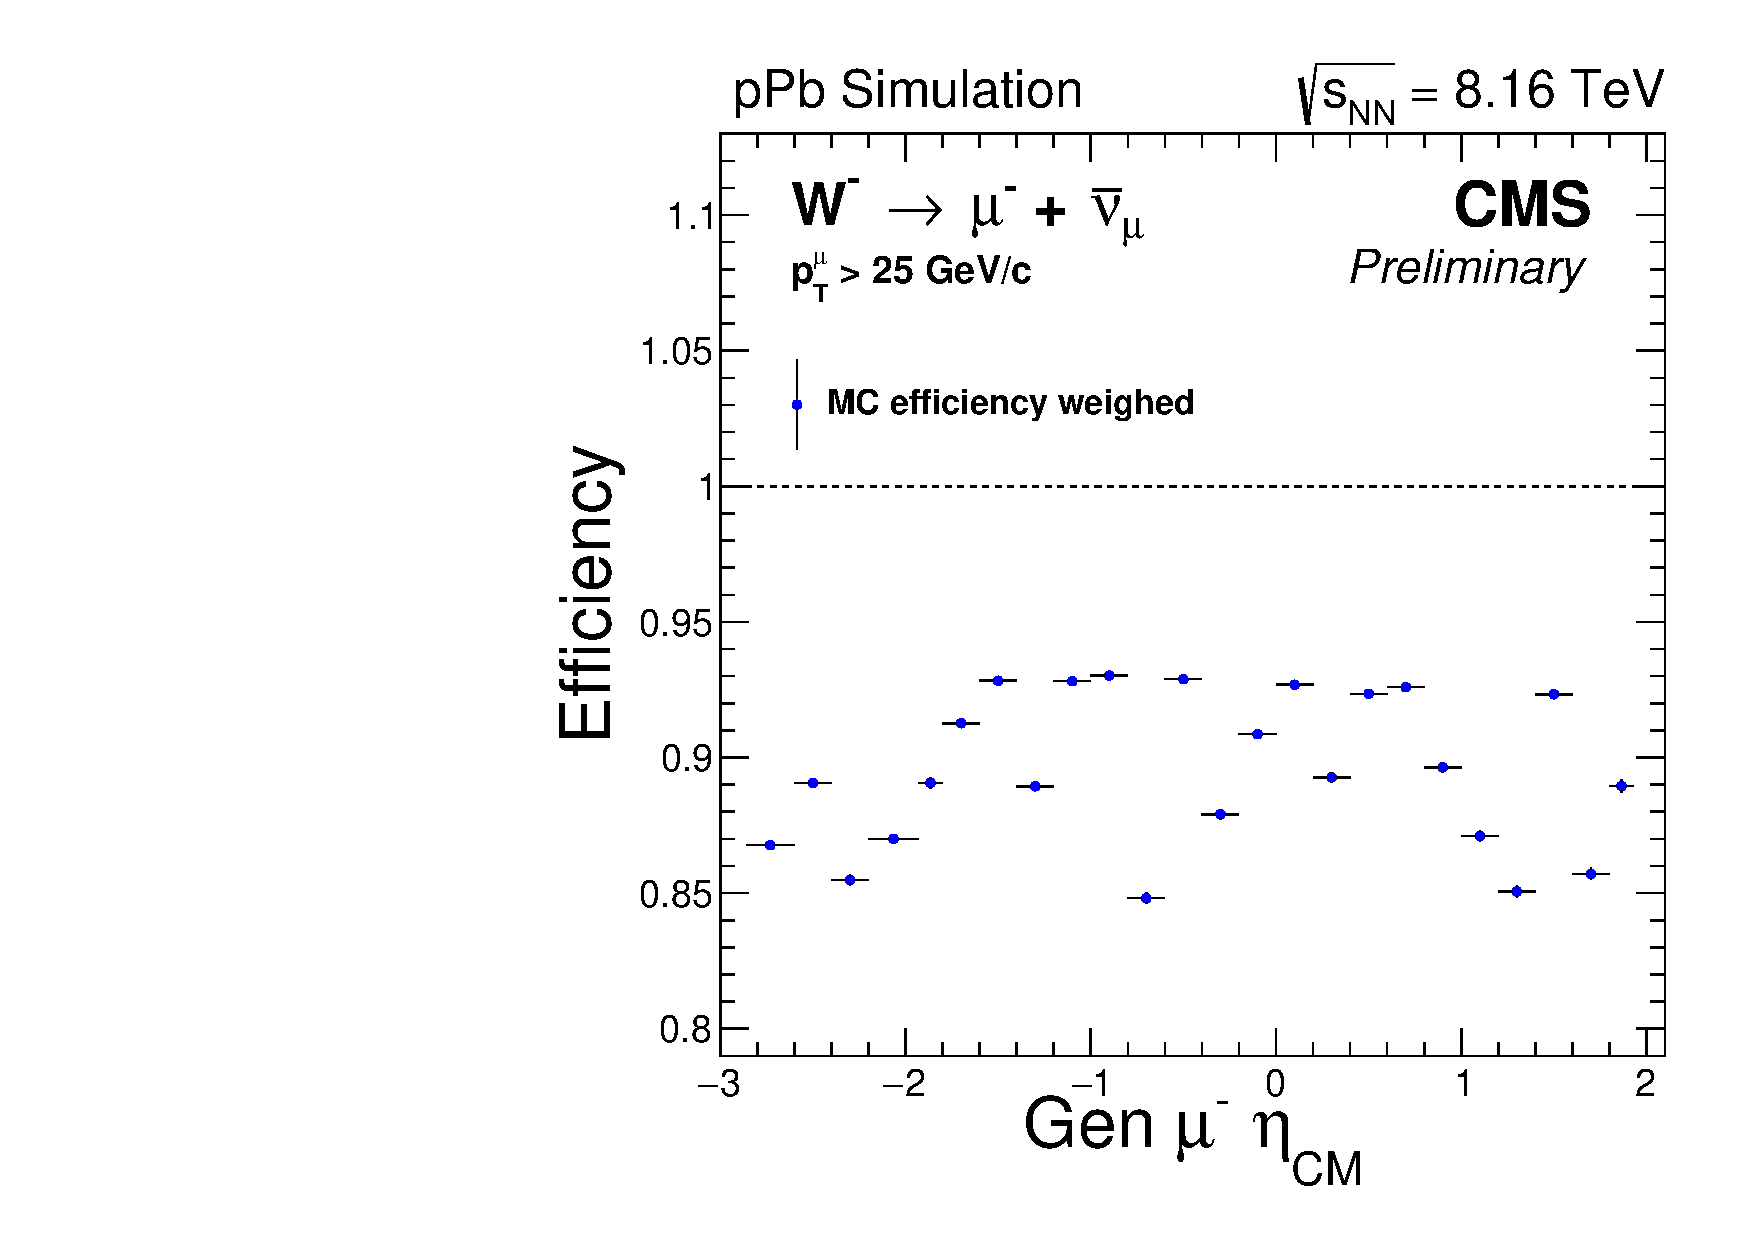
\includegraphics[width=0.45\textwidth]{Figures/WBoson/Analysis/Efficiency/eff1D_EtaCM_MC_WToMuNu_PA_Minus_Total_HFCorrOnly}
 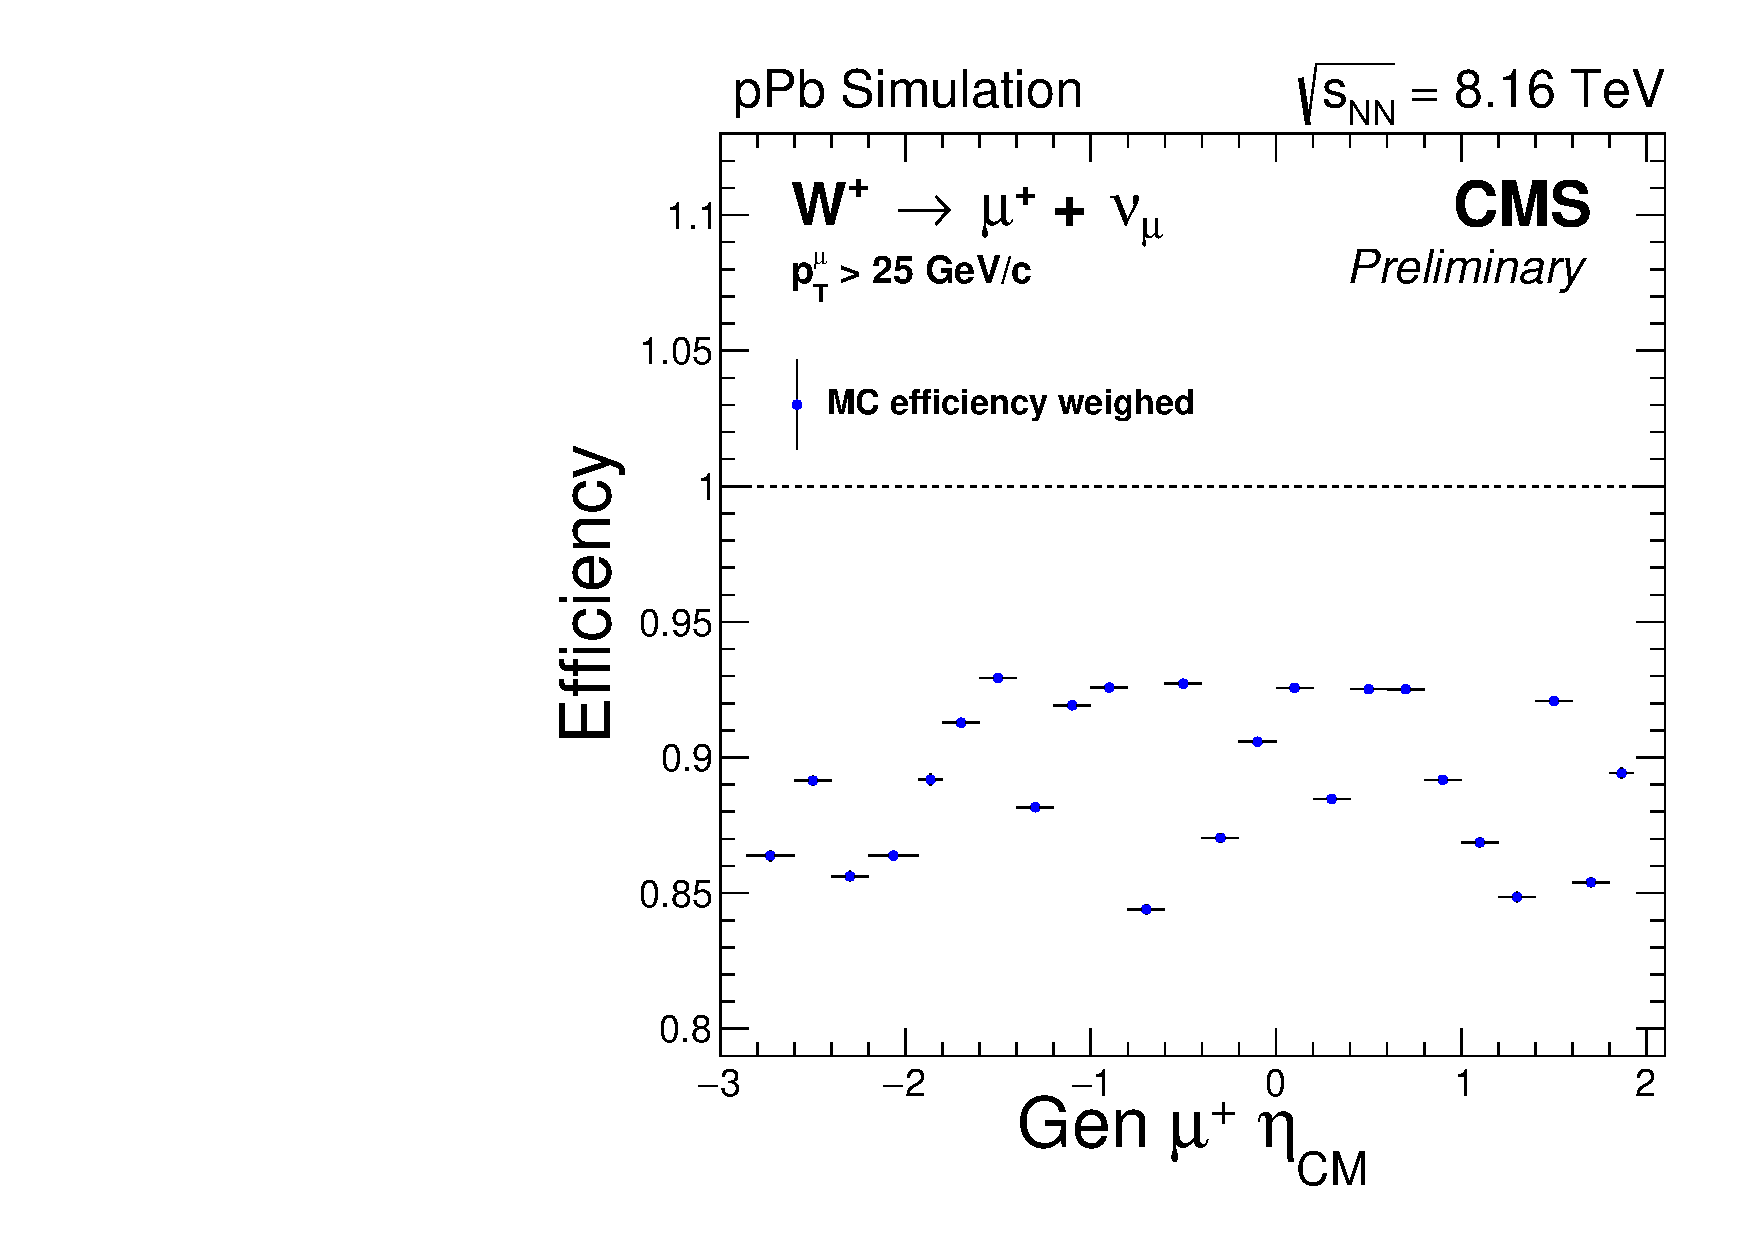
\includegraphics[width=0.45\textwidth]{Figures/WBoson/Analysis/Efficiency/eff1D_EtaCM_MC_WToMuNu_PA_Plus_Total_HFCorrOnly}
 \caption{Simulated signal efficiency derived from the \WToMuNu NLO simulations as a function of the generated muon \etaCM, separated in negative (left) and positive (right) charged muons. The distributions of the simulated HF energy and generated \Wb-boson \pt have been weighed.}
 \label{fig:MCTruthEfficiency}
\end{figure}

\subsubsection{Corrected signal efficiency}\label{sec:WBoson_Analysis_Efficiency_Corrected}

The simulation of the CMS detector is very precise but still far from fully describing all the detector conditions observed in real data. In order to compensate for the imperfections in the simulation, a set of data-to-MC corrections provided by the CMS heavy-ion (HIN) group are used to improve the estimation of the signal efficiency. These corrections are derived from the ratio of efficiencies measured in data and simulation using the tag-and-probe (TnP) method.

The tag-and-probe method is a data-driven technique widely used to compute efficiencies of physical objects, such as muons, produced from the decay of known mass resonances (e.g. \Z bosons). The main advantage of the TnP method is that it can be applied to data and simulation, allowing to asses the differences between the two.

\paragraph{Definition of the tag-and-probe efficiencies.} To study the different elements that enters in the reconstruction and selection of muons, the total muon efficiency is factorised in five different components, according to:

\begin{equation}
 \epsilon^{\mu} = \epsilon_{\text{STA}}\cdot\epsilon_{\text{TRK}}\cdot\epsilon_{\text{ID}}\cdot\epsilon_{\text{Trig}}\cdot\cdot\epsilon_{\text{Iso}}
\end{equation}

where each efficiency component is defined relative to the previous one, as described below:

\begin{itemize}
 \item $\epsilon_{\text{STA}}$ : represents the standalone-muon (STA) reconstruction efficiency. It is probed by tracker tracks and is derived by matching the probe to a standalone muon.
 \item $\epsilon_{\text{trk}}$ : represents the global muon tracking efficiency. It is probed by standalone muons and is derived by matching the probe to a global muon.
 \item $\epsilon_{\text{ID}}$ : represents the muon identification efficiency. It is probed by global muons and is determined by requiring that the probe satisfy the tight identification criteria defined in \sect{sec:WBoson_Analysis_Selection_MuonIdentification}.
 \item $\epsilon_{\text{trig}}$ : represents the muon trigger efficiency. It is probed by global muons passing the identification criteria, and it is determined by requiring that the probe is matched to the muon trigger.
 \item $\epsilon_{\text{iso}}$ : represents the muon isolation efficiency. It is probed by global muons passing the identification criteria and matched to the trigger, and it is computed by requiring that the probe pass the muon isolation requirement ($\iso < 0.15$).
\end{itemize}


\paragraph{Extraction of the tag-and-probe efficiencies.} For high-\pt muons ($\pt > 15$~\GeVc), the dimuon decay of \Z bosons is used to create a clean sample. In each event, a high-quality muon, called the \textit{tag}, is combined with the \textit{probe} of the efficiency being measured, to form a tag-probe pair within the \Z-boson mass window. The tag and the probe are required to have $\pt > 15$~\GeVc and be inside the acceptance of CMS ($|\etaLAB| < 2.4$). In addition, the tag is also required to satisfy the muon isolation and identification criteria, and be matched to the trigger.

The tag-probe pairs are separated into two samples depending on whether the probe pass the selection criteria under study. The efficiency is then determined by performing a simultaneous unbinned maximum likelihood fit to the tag-probe invariant mass distribution ($m_{\text{TP}}$) for failing and passing probes. The \ZToMuMu signal distributions are parametrised with a Voigt profile~\cite{Voigt} and the background distributions with an  exponential. The same procedure is performed for all efficiencies measured in data and simulation.

As an example, the fits to the tag-probe invariant mass distribution for passing and failing probes, used to measure the STA reconstruction efficiency, are shown in \fig{fig:TnPFits}.

\begin{figure}[htb!]
 \centering
 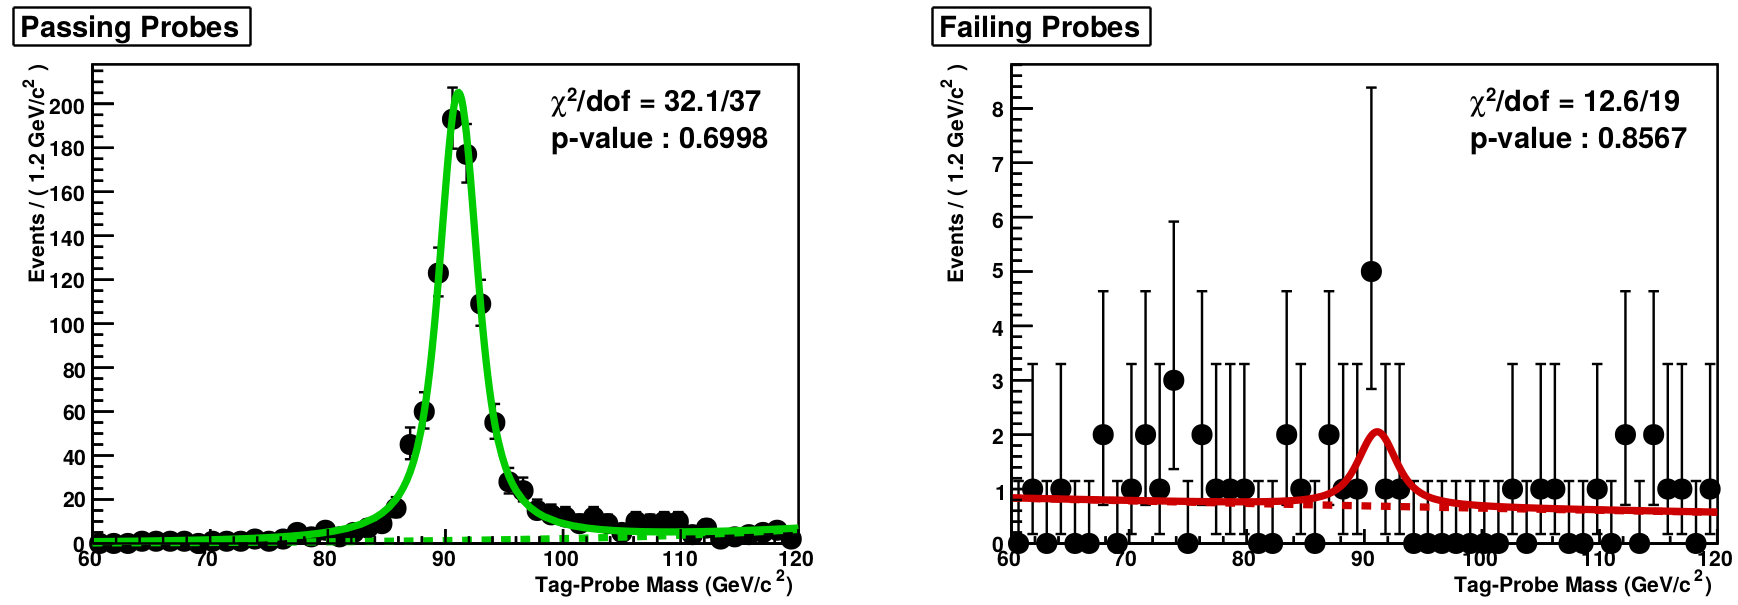
\includegraphics[width=0.9\textwidth]{Figures/WBoson/Analysis/Efficiency/TnP/TnPFit.png}
 \caption{Fits to the tag-probe invariant mass distribution for passing (left) and failing (right) probes, used to measure the STA reconstruction efficiency. The results correspond to the probe kinematic region: $\abs{\etaLAB}<2.4$ and $50 < \pt < 80$~\GeVc. Figures taken from the private Ref.~\cite{Muon_TnP_pPb}.}
 \label{fig:TnPFits}
\end{figure}


\paragraph{Results of the tag-and-probe efficiencies.} The STA reconstruction $\epsilon_{\text{STA}}$ and global muon tracking $\epsilon_{\text{trk}}$ efficiencies are found to be in very good agreement between data and simulation, and no correction is required for the simulated \WToMuNu efficiency.

In the case of the muon identification $\epsilon_{\text{ID}}$ and isolation $\epsilon_{\text{iso}}$ efficiencies, the results obtained from simulation are observed to disagree with those from data, as shown in  \fig{fig:TnPEfficiencyIDIso}. As a result, the efficiencies measured in data and simulation, as a function of the probed \pt, are fitted with: a linear function ($f_{\text{ID}}(\pt) = a\cdot\pt + b$) for muon identification and a displaced error function ($f_{\text{iso}}(\pt) = a\cdot\text{Erf}[(\pt - c)/b] + d$) for  muon isolation. The fits to the efficiencies are performed in three regions of probe \etaLAB, corresponding to: $\abs{\etaMuLAB} < 1.2$,   $1.2 < \abs{\etaMuLAB} < 2.1$ and  $2.1 < \abs{\etaMuLAB} < 2.4$. The ratio of the fitted functions extracted from the data and simulation efficiencies, for muon identification  ($w_{\text{ID}} = f^{\data}_{\text{ID}}\big/f^{\MC}_{\text{ID}}$) and for muon isolation ($w_{\text{iso}} = f^{\data}_{\text{iso}}\big/f^{\MC}_{\text{iso}}$), are used as TnP corrections for the simulated \WToMuNu efficiency.

\begin{figure}[htb!]
 \centering
 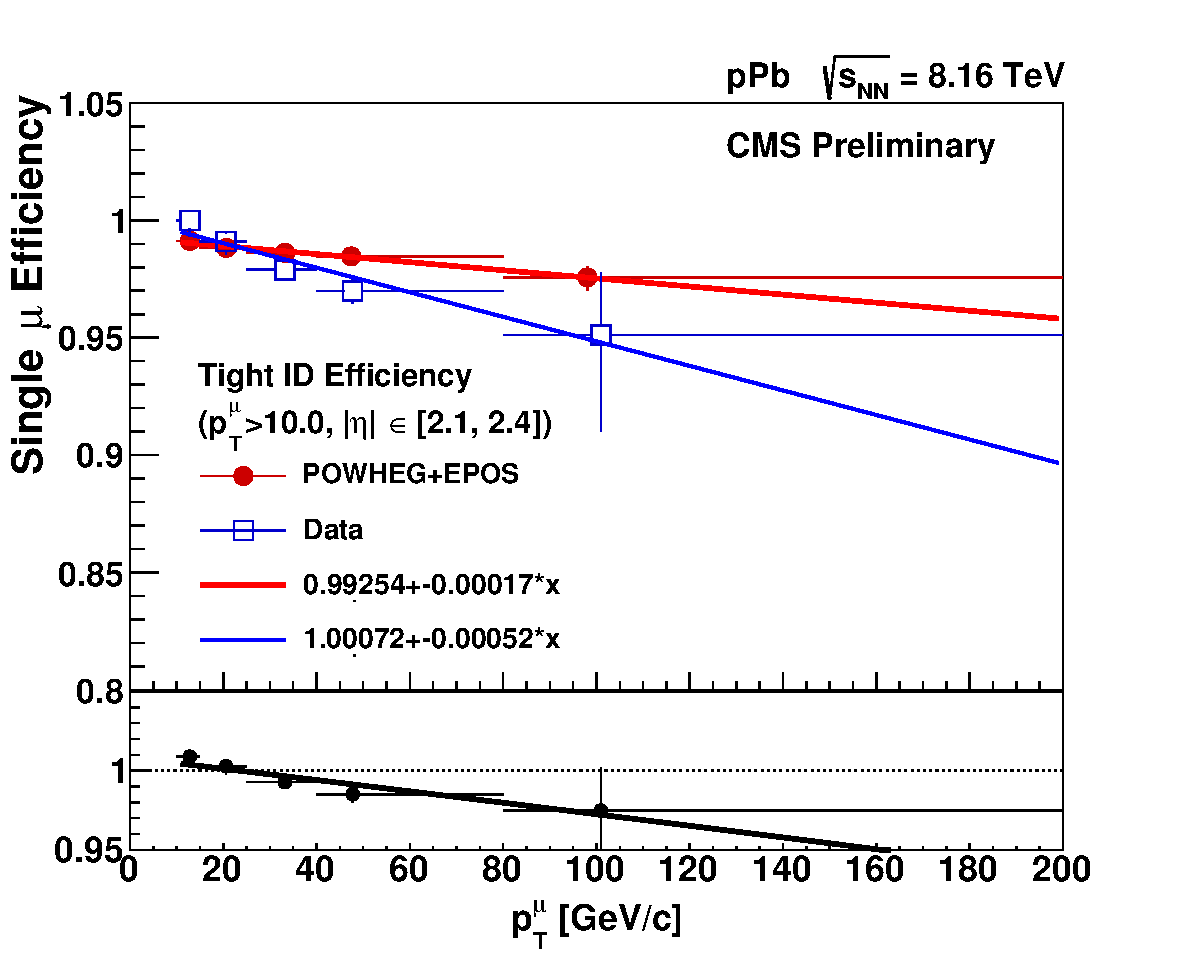
\includegraphics[width=0.45\textwidth]{Figures/WBoson/Analysis/Efficiency/TnP/tpTreeSF7_pPb_RD_MC_PT.pdf}
 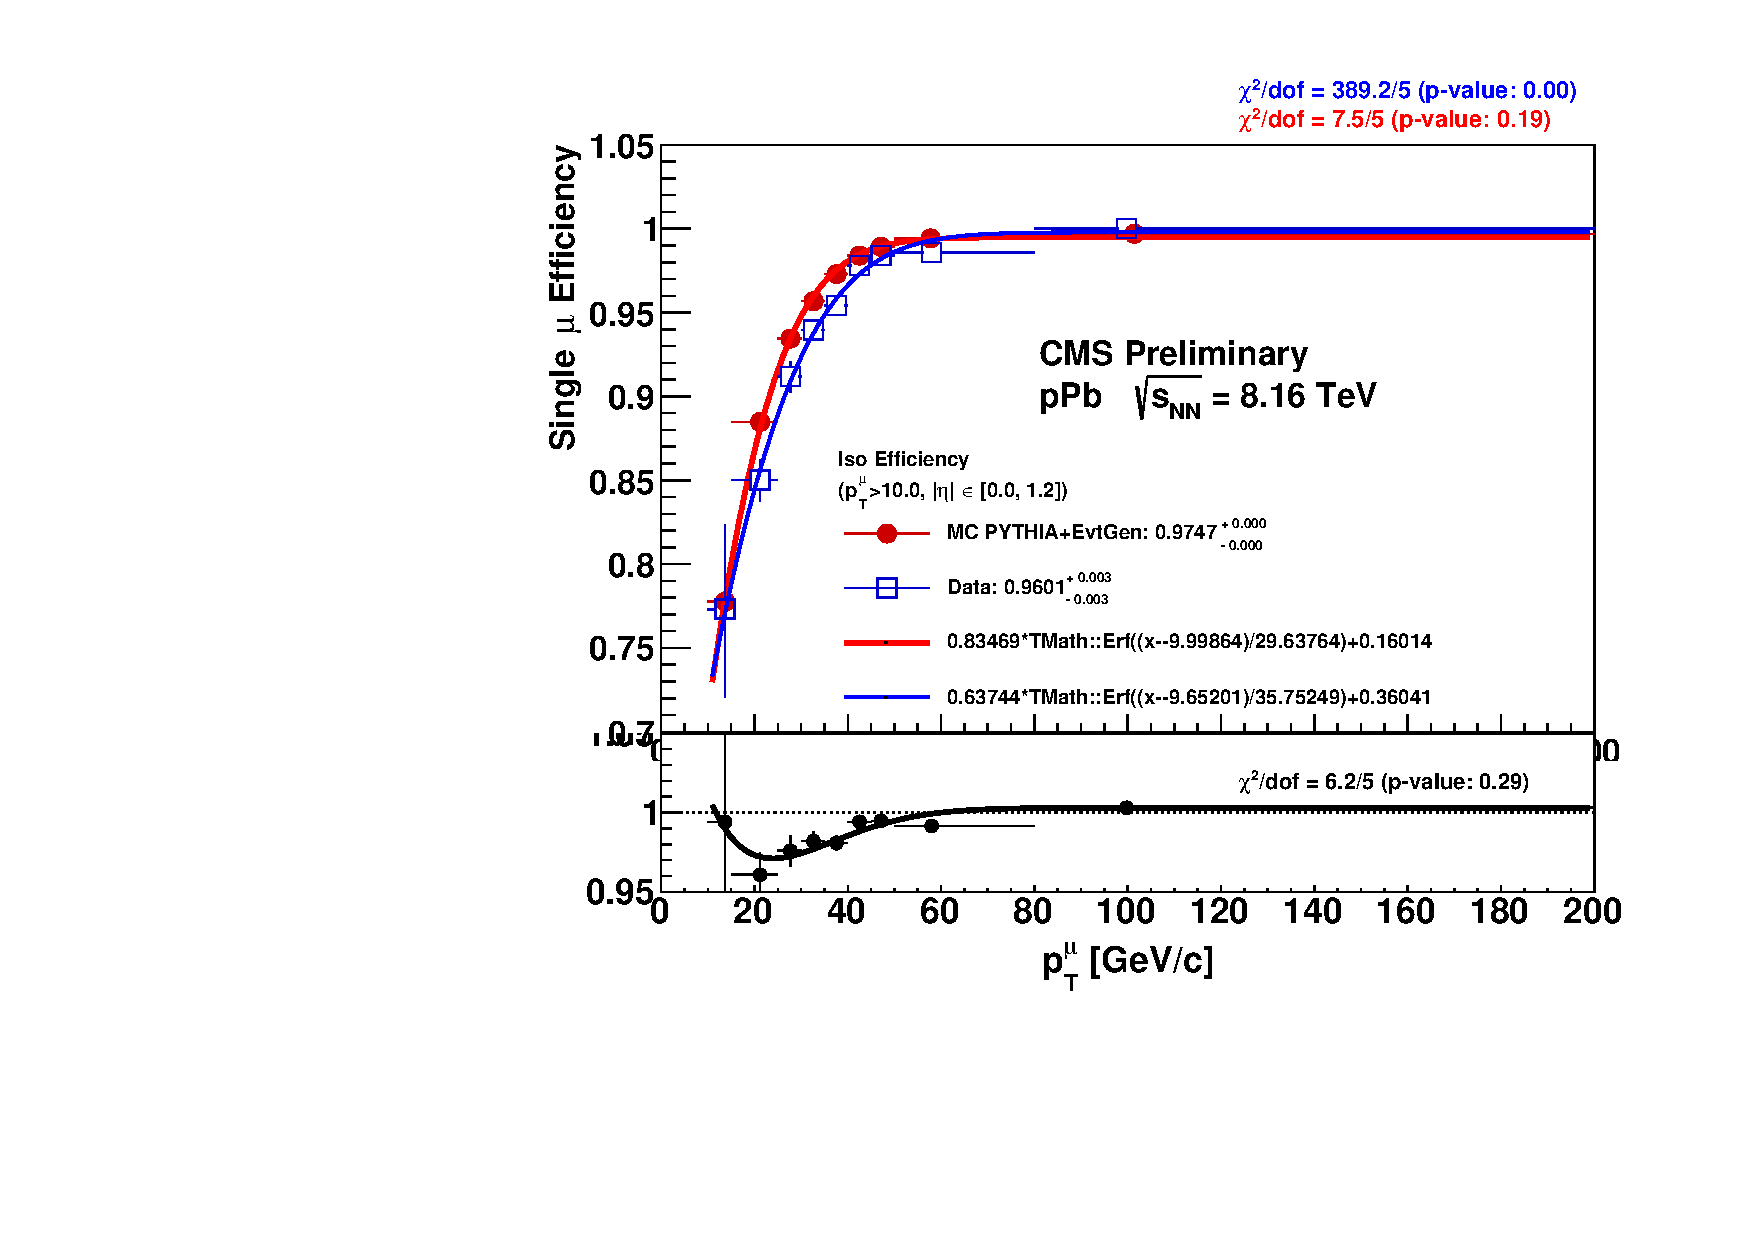
\includegraphics[width=0.45\textwidth]{Figures/WBoson/Analysis/Efficiency/TnP/tpTreeSF3_pPb_RD_MC_PT.pdf}
 \caption{Muon identification (left) and isolation (right) efficiencies extracted from data (blue) and simulation (red) using the TnP method, as a function of the probe \pt. The bottom panels show the data-to-simulation efficiency ratio. The results of the fits to the efficiencies are also shown. Figures taken from the private Ref.~\cite{Muon_TnP_pPb}.}
 \label{fig:TnPEfficiencyIDIso}
\end{figure}

The muon trigger efficiency $\epsilon_{\text{trig}}$ extracted from the simulation is seen to disagree with the results from data as a function of the probe \etaLAB, as presented in \fig{fig:TnPEfficiencyTrigger}. In this case, the ratio of the measured efficiency extracted from data and simulation ($w_{\text{trig}} = \epsilon^{\data}_{\text{ID}}\big/\epsilon^{\MC}_{\text{ID}}$), in each bin of probe \etaLAB, is used to correct the simulated \WToMuNu efficiency.

\begin{figure}[htb!]
 \centering
 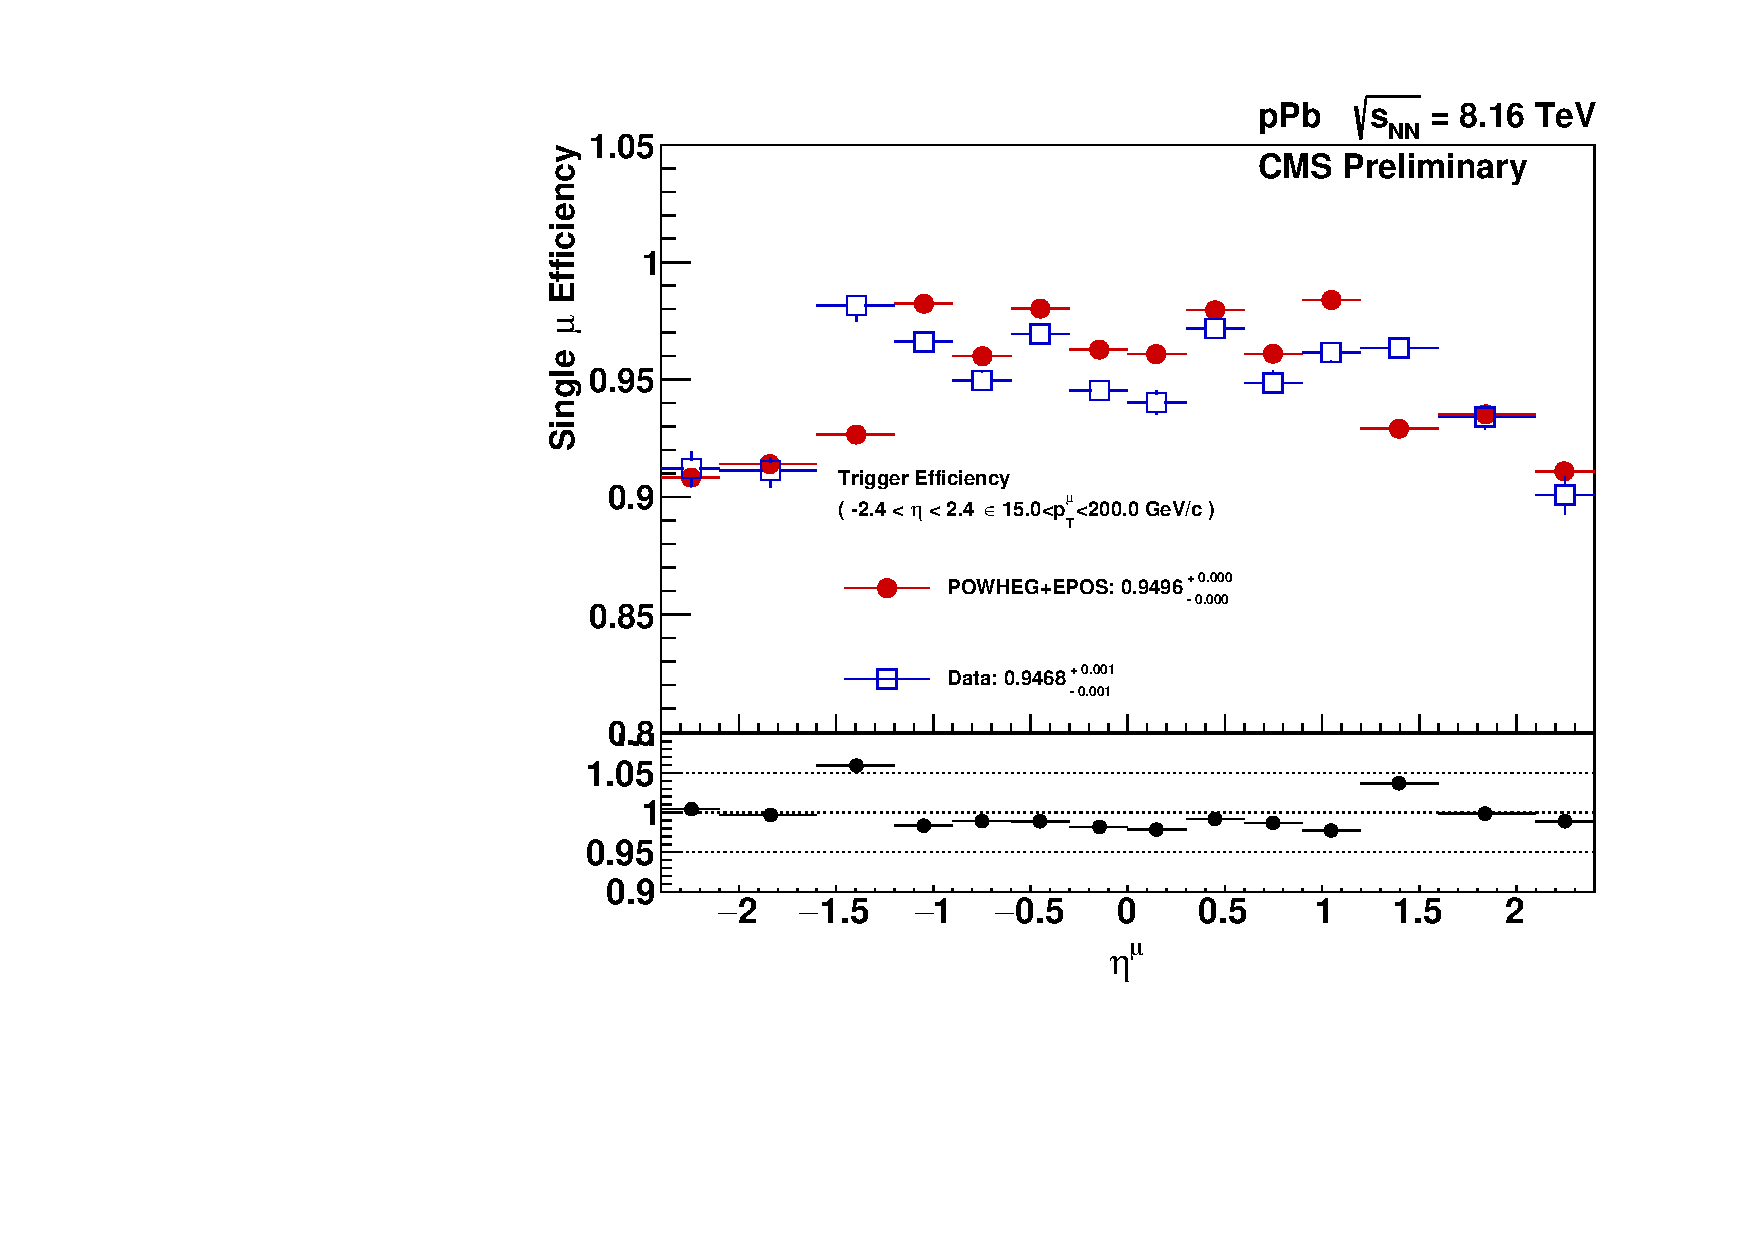
\includegraphics[width=0.45\textwidth]{Figures/WBoson/Analysis/Efficiency/TnP/tpTreeEff0_pPb_RD_MC_Eta.pdf}
 \caption{Muon trigger efficiency extracted from data (blue) and simulation (red) using the TnP method, as a function of the probe \etaLAB. The bottom panel shows the data-to-simulation efficiency ratio. Figure taken from the private Ref.~\cite{Muon_TnP_pPb}.}
 \label{fig:TnPEfficiencyTrigger}
\end{figure}

\paragraph{Correction of the signal efficiency.} The simulated signal efficiency is recomputed by weighing the offline muon yield per event using the TnP corrections provided by the CMS HIN group, for muon identification $w_{\text{ID}}$, trigger $w_{\text{trig}}$ and isolation $w_{\text{iso}}$, according to:

\begin{equation}
 \epsilon^{\mu^{\pm}}_{\corr} = \frac{\left[\sum\limits_{i=1}^{N_{\text{off}}^{\mu^{\pm}}} w_{\text{ID}}\left(\ptMu, \abs{\etaMuLAB}\right) \cdot w_{\text{trig}}\left(\etaLAB\right) \cdot w_{\text{iso}}\left(\ptMu, \abs{\etaMuLAB}\right)\right]}{N_{\gen,\pt>25}^{\mu^{\pm}}}
\end{equation}

where the TnP corrections are evaluated with the offline muon \pt and \etaLAB in each event, and the sum is performed over the simulated signal events.

\paragraph{Uncertainties of the tag-and-probe corrections.} The uncertainties associated to the TnP corrections are driven by the larger background and lower statistics present in data. As a result, only the uncertainties associated to the data efficiencies are propagated to the TnP corrections, while the simulation efficiencies  are fixed. The statistical and systematic components of the TnP correction uncertainties are estimated by performing the following set of variations:

\begin{itemize}

 \item (A) Statistical uncertainty for muon ID and isolation: estimated by generating a hundred sets of TnP corrections using pseudo-experiments. For each pseudo-experiment, the data efficiency points are randomly varied based on a Gaussian distribution of width equal to the statistical uncertainty of the efficiency points. The varied data efficiencies are then refitted providing new TnP corrections.

 \item (B) Statistical uncertainty for muon trigger: estimated with two sets of TnP corrections, determined by varying the data efficiency points up and down according to their statistical uncertainty.

 \item (C) Systematic uncertainty of the efficiency extraction: derived by refitting the tag-probe invariant mass distributions after varying the signal and background functional forms, and by extending the range of the \Z-boson mass window. These uncertainties are then propagated to the TnP corrections by varying the data efficiency points up and down by one standard deviation, producing two sets of TnP corrections.

 \item (D) Systematic uncertainty of the efficiency parametrisation for muon ID and isolation: estimated by using the ratio of the efficiency points from data and simulation ($w = \epsilon^{\data}\big/\epsilon^{\MC}$), instead of the fitted efficiency curves.

\end{itemize}

In addition, an uncertainty of $0.34\%$ is included to account for the impact of the different level of event activity present in data and simulation. This is derived by comparing the simulated muon isolation efficiency  before and after applying the HF energy weighing. Moreover, an uncertainty of $0.6\%$ is also added to account for possible mismodelling of the STA reconstruction efficiency, determined from the maximum difference between  data and simulation.

The uncertainties of the TnP corrections are propagated to the signal efficiency in two ways:

\begin{itemize}
 \item For the hundred TnP corrections described in (A): the signal efficiency is recomputed with each of the TnP corrections and the RMS of the hundred signal efficiencies obtained is then taken as the uncertainty on the signal efficiency.
 \item For the up and down variations used in (B), (C) and (D): the uncertainty on the signal efficiency is determined from the maximum difference between the signal efficiency recomputed with the nominal and each of the varied TnP corrections.

\end{itemize}

The total uncertainty on the signal efficiency due to TnP corrections, is obtained by summing in quadrature the uncertainties from (A), (B), (C) and (D). The additional relative uncertainties of 0.34\% and 0.6\% are also included.


\paragraph{Results of the signal efficiency correction.} The corrected signal efficiency is shown in \fig{fig:CorrEfficiency}, including the  uncertainties due to TnP correction. 

\begin{figure}[htb!]
 \centering
 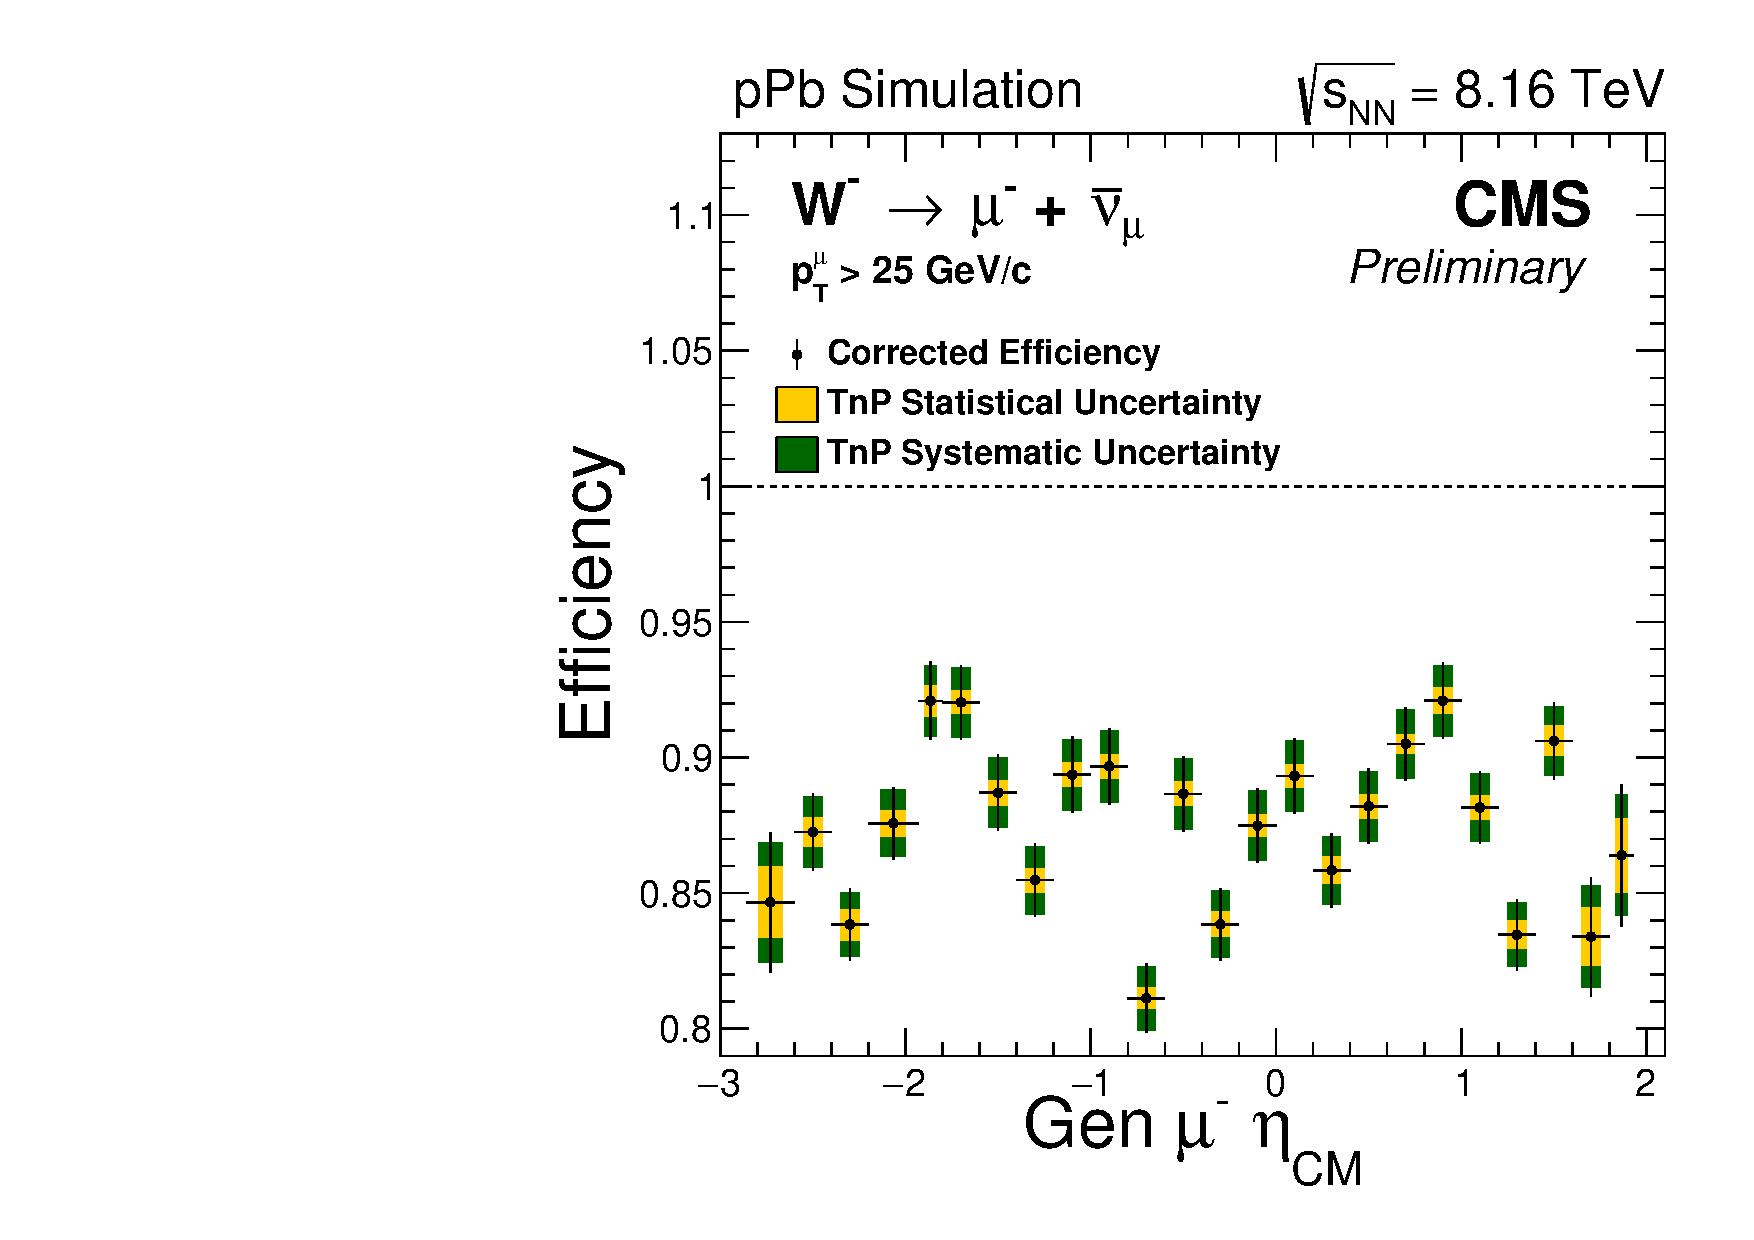
\includegraphics[width=0.45\textwidth]{Figures/WBoson/Analysis/Efficiency/eff1D_EtaCM_MC_WToMuNu_PA_Minus_Total_TnP_Nominal}
 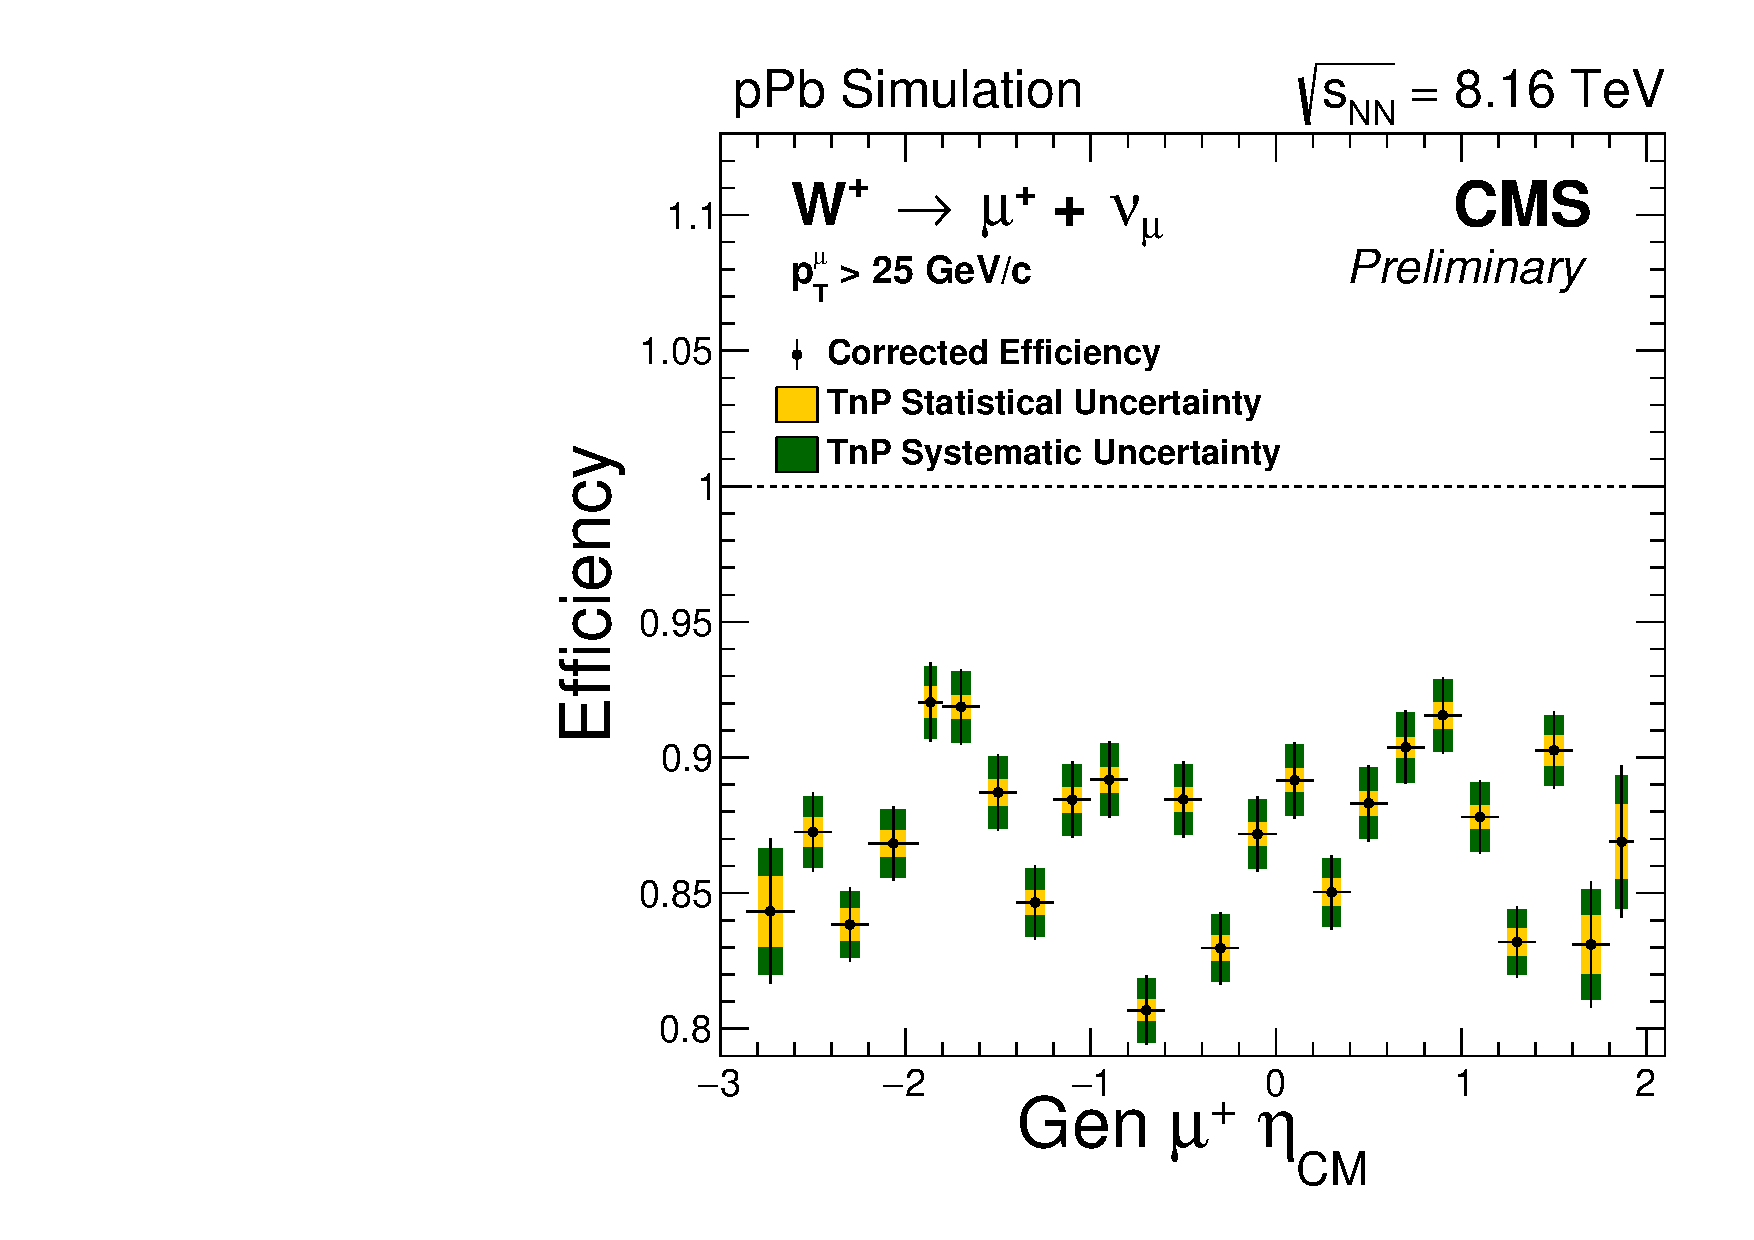
\includegraphics[width=0.45\textwidth]{Figures/WBoson/Analysis/Efficiency/eff1D_EtaCM_MC_WToMuNu_PA_Plus_Total_TnP_Nominal}
 \caption{Corrected signal efficiency as a function of the generated muon \etaCM, separated in negative (left) and positive (right) charged muons. The yellow and green boxes represents the uncertainty on the signal efficiency due to the TnP statistics and systematics, respectively.}
 \label{fig:CorrEfficiency}
\end{figure}

The relative difference between the corrected and the simulated signal efficiencies ($(\epsilon_{\corr}-\epsilon_{\MC})\big/\epsilon_{\MC}$), is presented in \tab{tab:compEfficiency_WToMu_PA} as a function of the generated \etaCM. The largest variation due to the TnP corrections is found to be $4.7\%$.

\begin{table}[htb!]
  \centering
  %\renewcommand{\arraystretch}{1.5}
  \begin{tabular}{|c|*2c|}
    \hline
    $\etaMuCM$ Range & $\mu^{-}$ $\frac{\epsilon_{\corr}-\epsilon_{\MC}}{\epsilon_{\MC}}$ [\%] & $\mu^{+}$ $\frac{\epsilon_{\corr} - \epsilon_{\MC}}{\epsilon_{\MC}}$ [\%]\\
    \hline\hline
    $-$2.86 , $-$2.60 & -2.4 & -2.4\\
    \hline
    $-$2.60 , $-$2.40 & -2.0 & -2.1\\
    \hline
    $-$2.40 , $-$2.20 & -1.9 & -2.1\\
    \hline
    $-$2.20 , $-$1.93 & 0.7 & 0.5\\
    \hline
    $-$1.93 , $-$1.80 & 3.4 & 3.2\\
    \hline
    $-$1.80 , $-$1.60 & 0.8 & 0.6\\
    \hline
    $-$1.60 , $-$1.40 & -4.4 & -4.5\\
    \hline
    $-$1.40 , $-$1.20 & -3.9 & -4.0\\
    \hline
    $-$1.20 , $-$1.00 & -3.7 & -3.8\\
    \hline
    $-$1.00 , $-$0.80 & -3.6 & -3.7\\
    \hline
    $-$0.80 , $-$0.60 & -4.4 & -4.4\\
    \hline
    $-$0.60 , $-$0.40 & -4.6 & -4.6\\
    \hline
    $-$0.40 , $-$0.20 & -4.6 & -4.7\\
    \hline
    $-$0.20 , $+$0.00 & -3.7 & -3.8\\
    \hline
    $+$0.00 , $+$0.20 & -3.6 & -3.7\\
    \hline
    $+$0.20 , $+$0.40 & -3.8 & -3.9\\
    \hline
    $+$0.40 , $+$0.60 & -4.5 & -4.6\\
    \hline
    $+$0.60 , $+$0.80 & -2.3 & -2.3\\
    \hline
    $+$0.80 , $+$1.00 & 2.7 & 2.7\\
    \hline
    $+$1.00 , $+$1.20 & 1.2 & 1.1\\
    \hline
    $+$1.20 , $+$1.40 & -1.9 & -2.0\\
    \hline
    $+$1.40 , $+$1.60 & -1.9 & -2.0\\
    \hline
    $+$1.60 , $+$1.80 & -2.7 & -2.7\\
    \hline
    $+$1.80 , $+$1.93 & -2.9 & -2.8\\
    \hline
  \end{tabular}
  \caption{Relative difference between the corrected and simulated signal efficiencies as a function of the generated muon $\eta_{CM}$, separated in negative and positive charged muons.}
  \label{tab:compEfficiency_WToMu_PA}
\end{table}





% END OF SUBSECTION


\subsection{Signal extraction}\label{sec:WBoson_Analysis_SignalExtraction}

The signal and background event yields are extracted by fitting the \ptmiss distribution from data. The background events correspond to high-\pt muons that satisfy the signal selection criteria and are not produced from a direct decay of a \Wb boson. A brief description of the background sources considered in this analysis is given below:

\begin{itemize}

 \item QCD jet: constitute high-\pt muons produced from semi-leptonic decays of heavy-flavour hadrons formed within jets. Such muons are generally surrounded by a large hadronic activity and their contribution is significantly suppressed by selecting isolated muons ($\iso < 0.15$). However, muons from hadron decays can sometimes pass the isolation criteria and thus, a small fraction of the QCD jet background remains in the signal region.

 \item $\DYToMuMu$: a high-\pt muon produced from a \Z-boson decay or Drell--Yan. The contribution from this process is suppressed by applying the \DYToMuMu veto, which excludes events containing at least one pair of well-identified isolated muons, each with $\pt > 15$~\GeVc. The \DYToMuMu events, in which one of the two muons is produced outside of the CMS coverage ($\abs{\etaLAB}<$ 2.4) or does not satisfy the muon selection criteria, survive the veto. Such events are expected to contribute more in the CMS endcap regions ($|\eta| > 2.0$), where one of the muons from the \DYToMuMu decay escape the detector producing a large \ptmiss.

 \item $\ttbar\rightarrow\mu\nu_{\mu}+X$: a high-\pt muon from semi-leptonic decays of top (anti-)quarks. The inclusive cross section of top-quark pair production in \pPb at $\sqrtsnn = \SI{8.16}{\TeV}$, has been measured by the CMS collaboration to be $\sigma_{\ttbar} = 45 \pm 8~\nbinv$~\cite{HIN-17-002}. The \ttbar process is expected to have a very small impact in the signal region due its small inclusive cross section and its branching ratio (13.4\%) to muons~\cite{PDG}.

 \item $\WToTauNu \rightarrow\mu\nu_{\mu} + X$: consists of the leptonic decay of a \Wb boson into a \PGt lepton, which then decays into a high-\pt muon.

 \item $\DYToTauTau\rightarrow\mu\nu_{\mu}+X$: corresponds to a ditau decay of a \Z boson or virtual photon, where one of the \PGt leptons then decays into a high-\pt muon.
 
\end{itemize}

The largest source of background in the signal region correspond to QCD jets which represents approximately 18\% of events in data. Among the electroweak background processes, the dominant one is the \DYToMuMu background. The electroweak background amounts to roughly 12\% of the events in the signal region, divided as: \DYToMuMu ($9\%$), \WToTauNu ($2\%$) and \DYToTauTau ($1\%$). The \ttbar background contributes roughly $0.5\%$ of  events. Other electroweak processes such as double boson decays ($\Wb\Wb$, $\Wb\Z$ and $\Z\Z$) have been checked to contribute less than 0.03\%, so they are not considered.

The shape of the QCD jet background is modelled using a functional form derived from data as explained in \sect{sec:WBoson_Analysis_SignalExtraction_QCDBackground} and the shapes of the signal, \ttbar background and electroweak background are estimated using the \ptmiss distribution from simulations, as described in \sect{sec:WBoson_Analysis_SignalExtraction_EWKBackground}. \sect{sec:WBoson_Analysis_SignalExtraction_FitModel} introduces the model used to extract the signal. The event yields obtained from the fits are presented in \sect{sec:WBoson_Analysis_SignalExtraction_RawYields} and corrected for efficiency in \sect{sec:WBoson_Analysis_SignalExtraction_CorrectedYields}.

\subsubsection{Modelling of the QCD jet background}\label{sec:WBoson_Analysis_SignalExtraction_QCDBackground}

The QCD jet background cannot be simulated reliably in \RunpPb collisions due to the imprecise knowledge of the production cross sections and nuclear modifications of hadrons, and the inaccurate modelling of the event activity. Thus, a data-driven approach is used to determine the QCD jet shape.

The overall procedure consist of the following steps: first parametrise the \ptmiss shape of the QCD jet background in a region dominated by non-isolated muons, then determine the dependence of the QCD jet functional form with respect to the muon isolation and finally extrapolate the QCD jet shape to low muon isolation values, namely in the signal region.

The shape of the QCD jet background is parametrised by a modified Rayleigh distribution, defined as:

\begin{equation}
 f_{\text{QCD}}\left(\ptmiss\right) = \ptmiss{\cdot}\exp\left(-\frac{\left(\ptmiss\right)^{2}}{2\left( \sigma_{0} + \sigma_{1}\cdot\ptmiss + \sigma_{2}\cdot\left( \ptmiss \right)^{2} \right)^{2}} \right)
 \label{eq:QCD_Nominal}
\end{equation}

where $\sigma_{0}$, $\sigma_{1}$, and $\sigma_{2}$ are free parameters extracted by performing an unbinned maximum-likelihood fit to the \ptmiss distribution in a control sample from data. The events in the control sample are selected by applying all signal selection requirements, except the muon isolation cut. The fits are performed separately for positive and negative charged muon events.

To derive the muon isolation dependence of the QCD jet background parameters, the \ptmiss spectrum in the control sample is fitted with the QCD jet functional form, in five bins of the muon isolation variable with the following boundaries: [ 0.4 , 0.5 , 0.6 , 0.7 , 0.8 , 0.9 ]. Lower muon isolation values ($\iso < 0.4$) are discarded, due to the large contamination from weak boson decays. The results of the QCD jet background fits, corresponding to the lowest and highest muon isolation regions, are shown in \fig{fig:QCD_Fits}.

\begin{figure}[htb!]
 \centering
  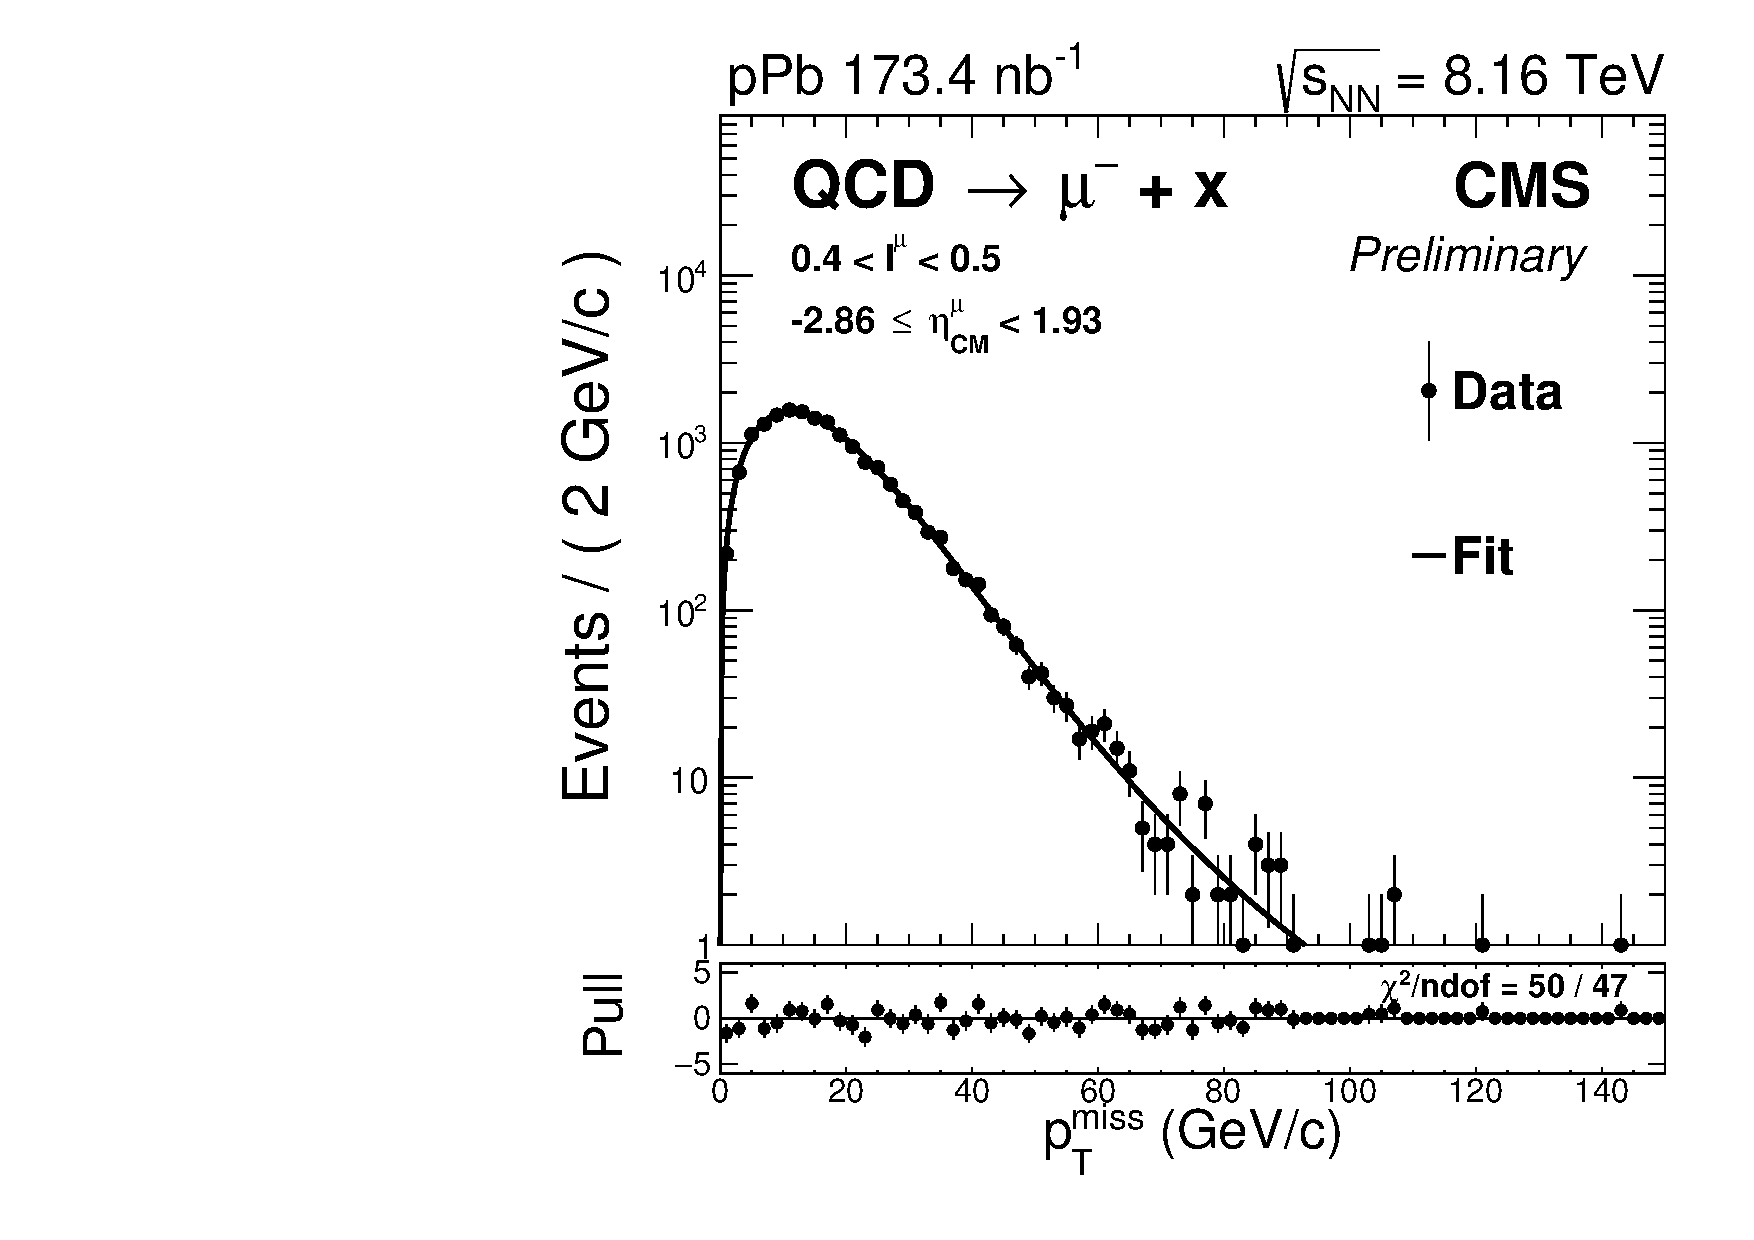
\includegraphics[width=0.45\textwidth]{Figures/WBoson/Analysis/SignalExtraction/QCD_Template/DATA/PLOT_MET_DATA_QCDToMuMi_PA_Model_ModifiedRayleigh_MuEtaCM_-286_193_MuIso_40_50.pdf}
  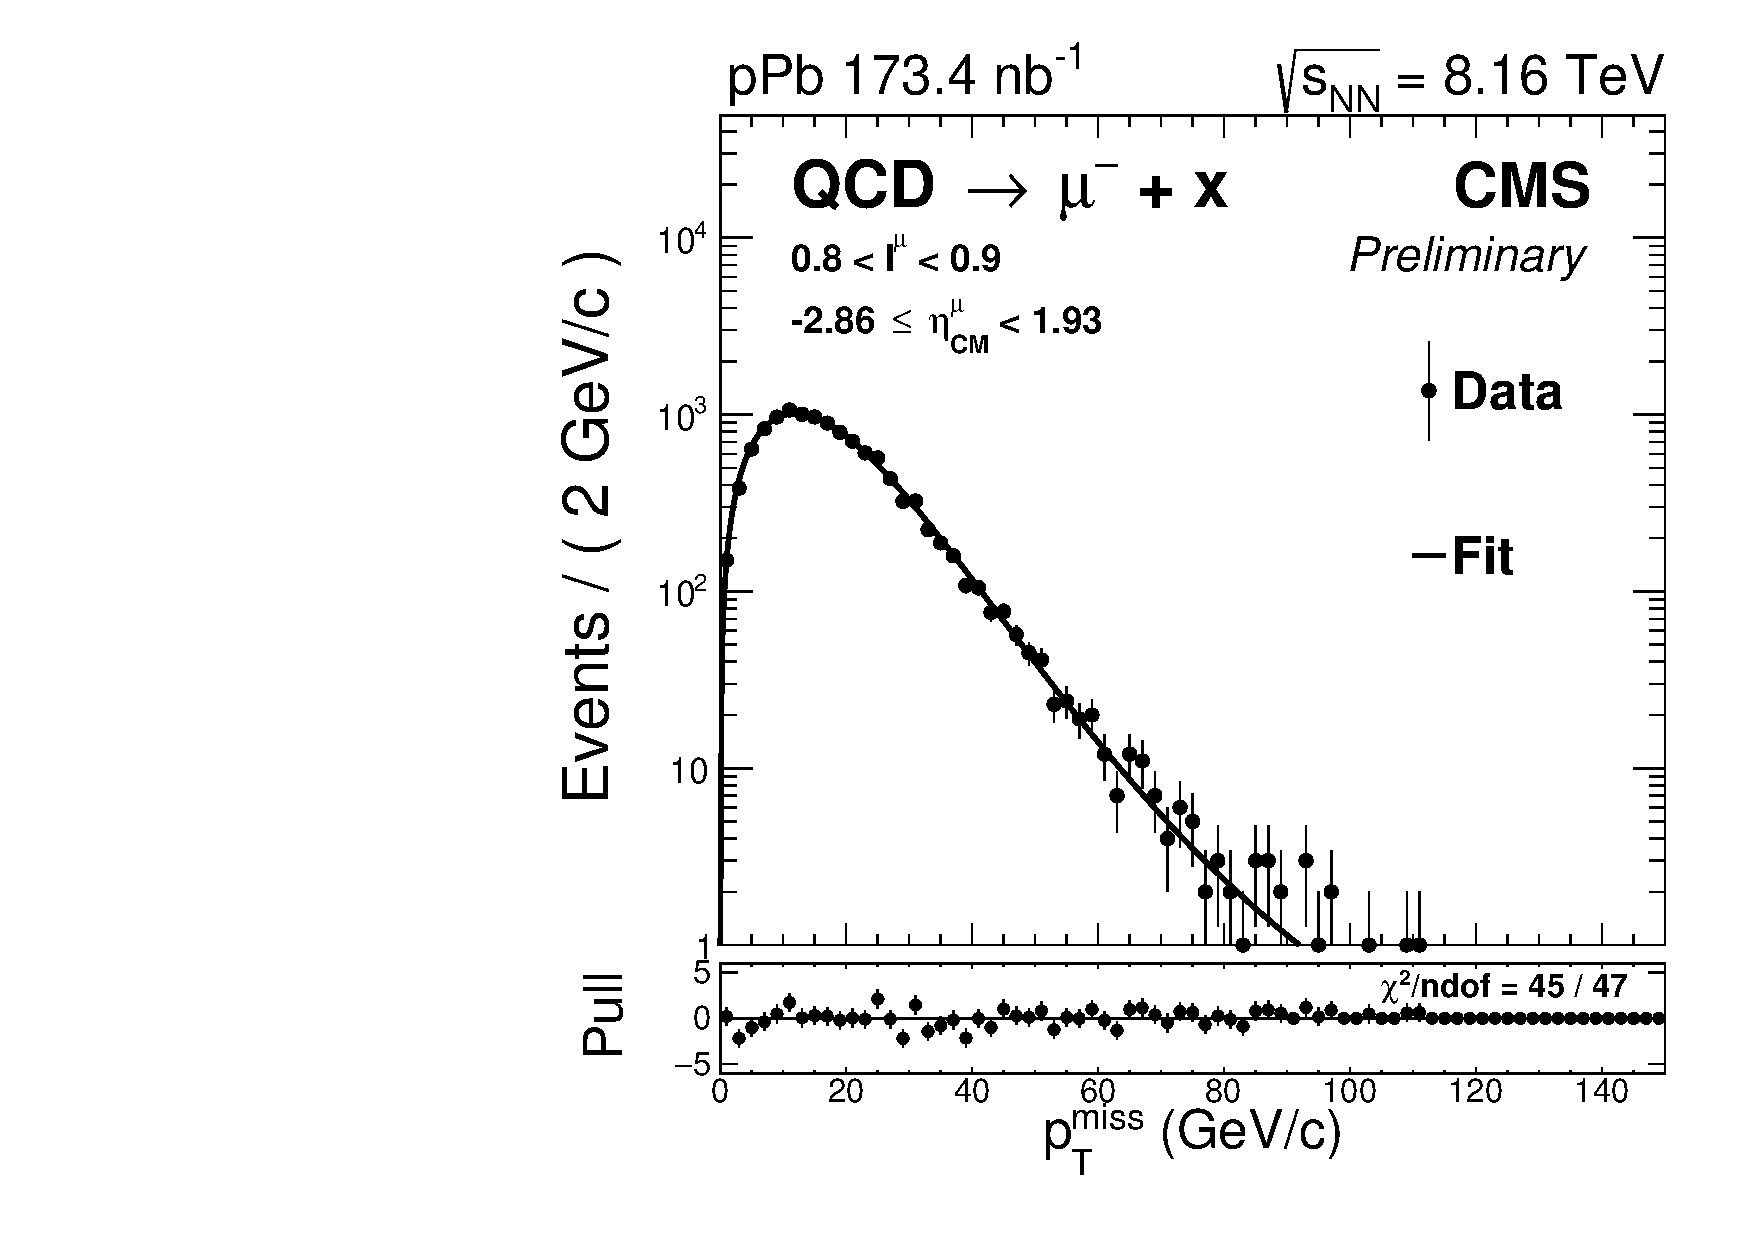
\includegraphics[width=0.45\textwidth]{Figures/WBoson/Analysis/SignalExtraction/QCD_Template/DATA/PLOT_MET_DATA_QCDToMuMi_PA_Model_ModifiedRayleigh_MuEtaCM_-286_193_MuIso_80_90.pdf}\\
  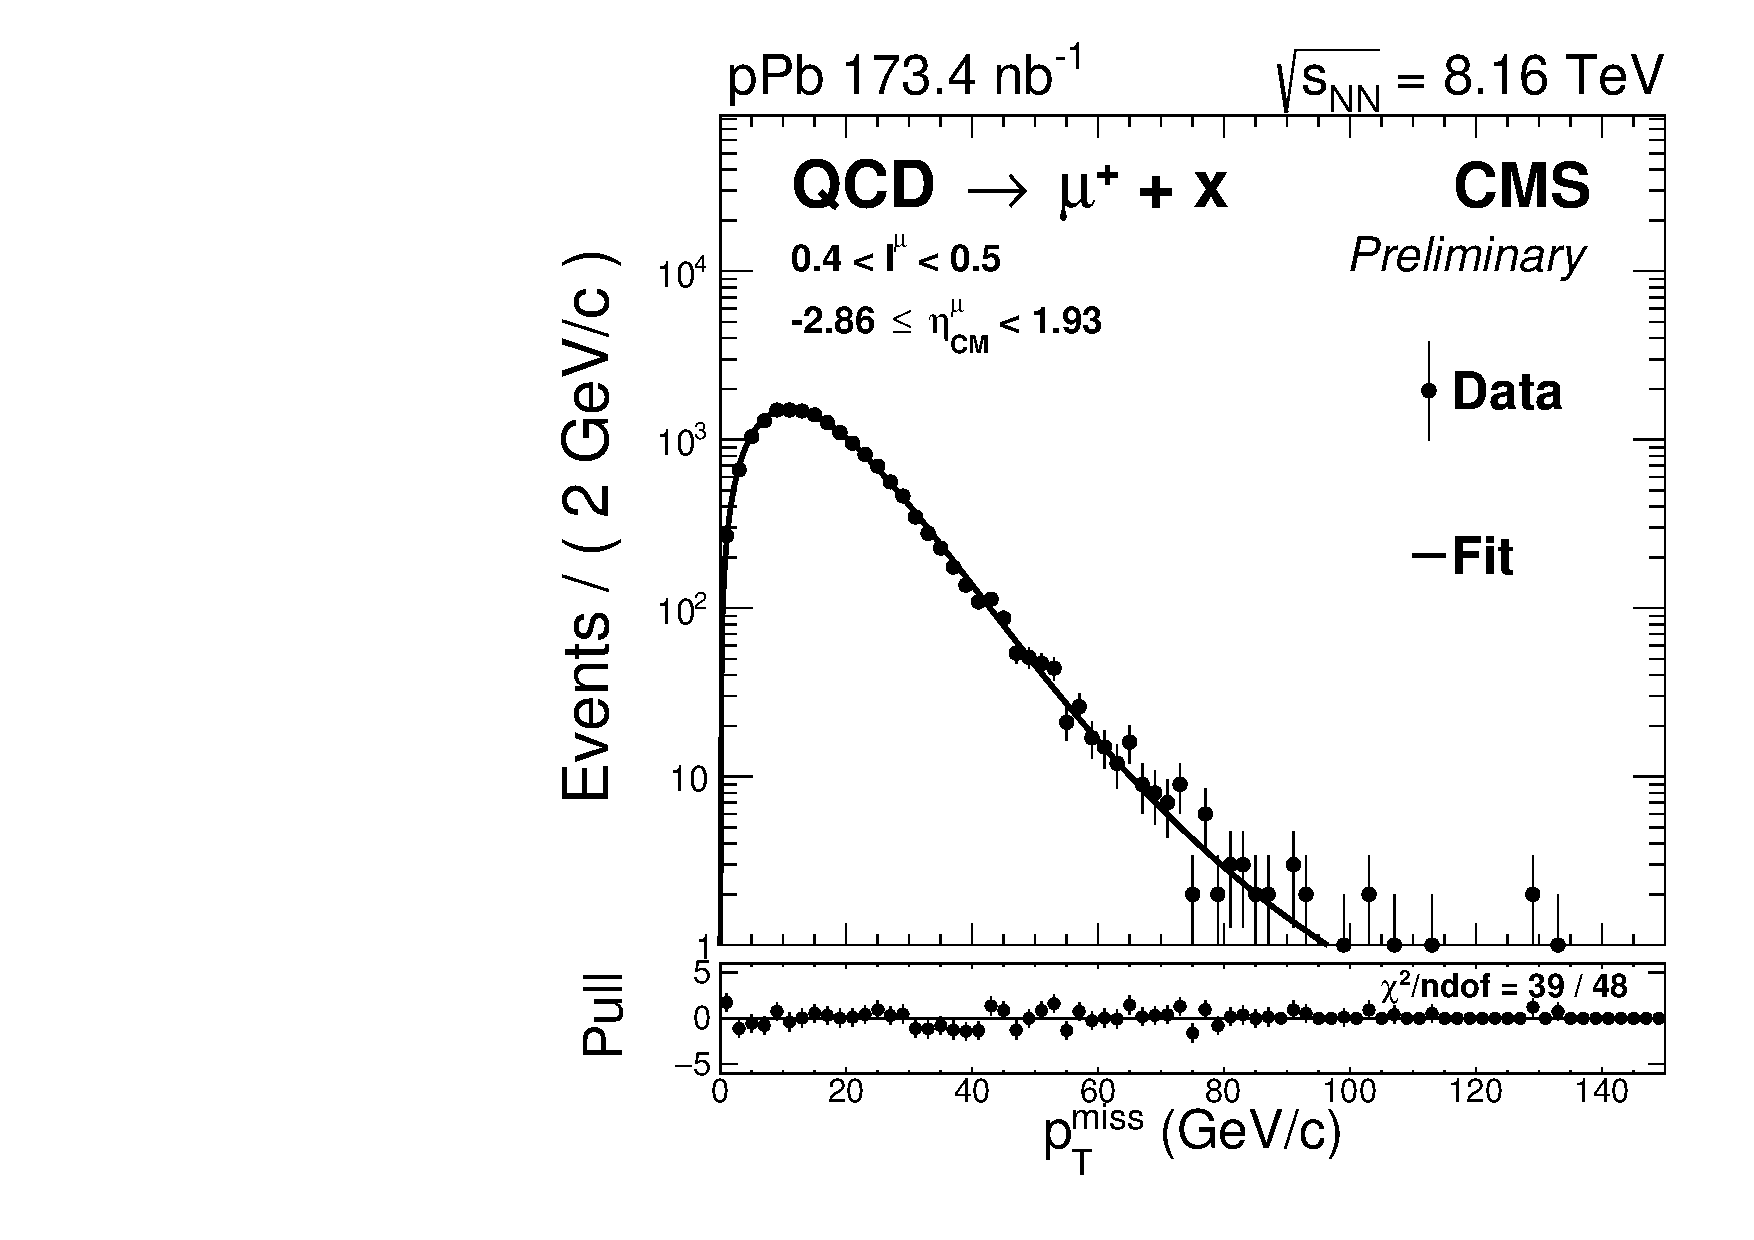
\includegraphics[width=0.45\textwidth]{Figures/WBoson/Analysis/SignalExtraction/QCD_Template/DATA/PLOT_MET_DATA_QCDToMuPl_PA_Model_ModifiedRayleigh_MuEtaCM_-286_193_MuIso_40_50.pdf}
  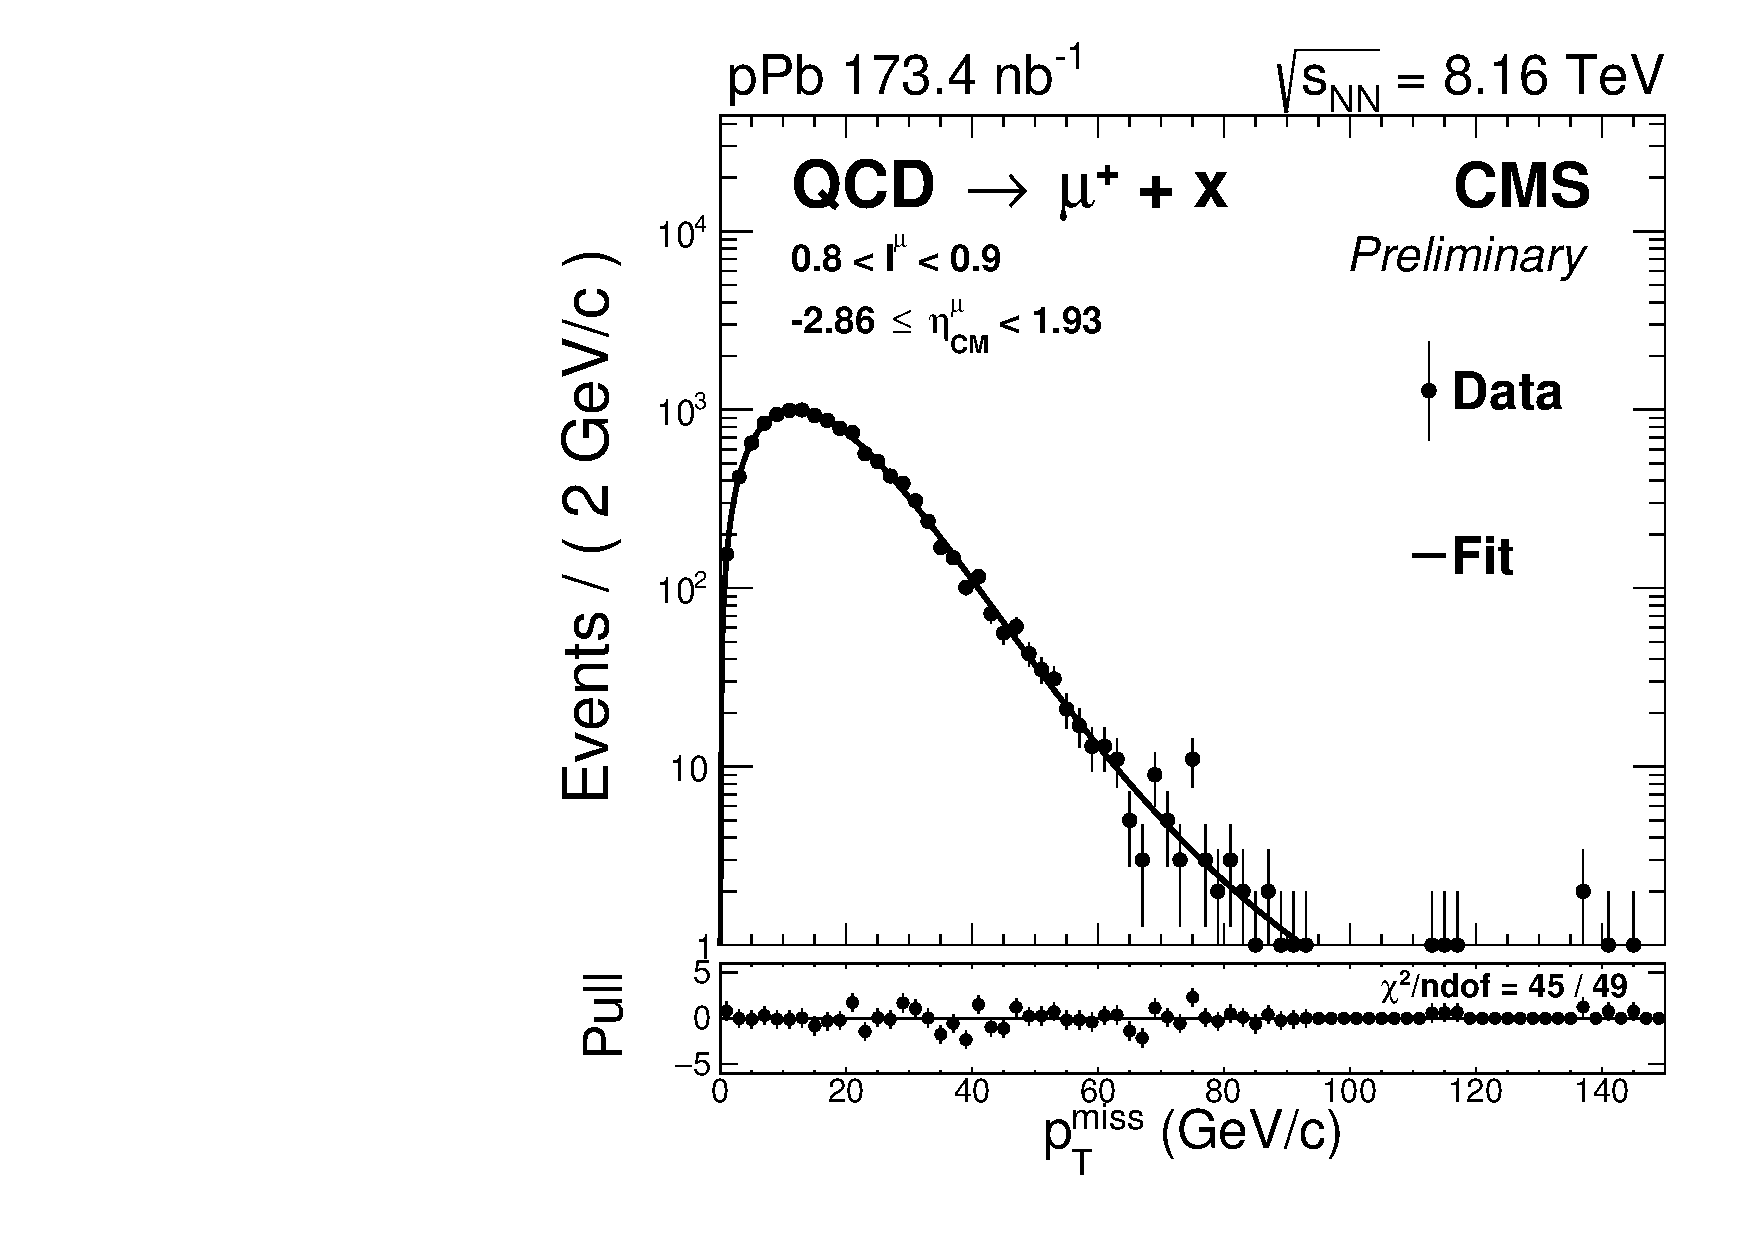
\includegraphics[width=0.45\textwidth]{Figures/WBoson/Analysis/SignalExtraction/QCD_Template/DATA/PLOT_MET_DATA_QCDToMuPl_PA_Model_ModifiedRayleigh_MuEtaCM_-286_193_MuIso_80_90.pdf}
 \caption{QCD jet background fits to the \ptmiss distribution in a control sample of non-isolated muon events  corresponding to the muon isolation bins: $0.4 < \iso < 0.5$ (left) and $0.8 < \iso < 0.9$ (right). The results are shown for positive (top) and negative (bottom) charged muons separately.}
 \label{fig:QCD_Fits}
\end{figure}

The QCD background parameters $\sigma_{0}$, $\sigma_{1}$, and $\sigma_{2}$, are extracted from the fits to the \ptmiss spectrum in each muon isolation bin, and their profile as a function of \iso is observed to be well described by a linear function, given by:

\begin{equation}
 \sigma_{i}\left(\iso\right) = \hat{\sigma}_{i} + s_{i}{\cdot}\iso
\end{equation}

where $\hat{\sigma}_{i}$ and $s_{i}$ are free parameters extracted separately for each QCD background parameter. The outcome of the linear fits is shown in \fig{fig:QCD_Extrapolation}.

\begin{figure}[htb!]
 \centering
 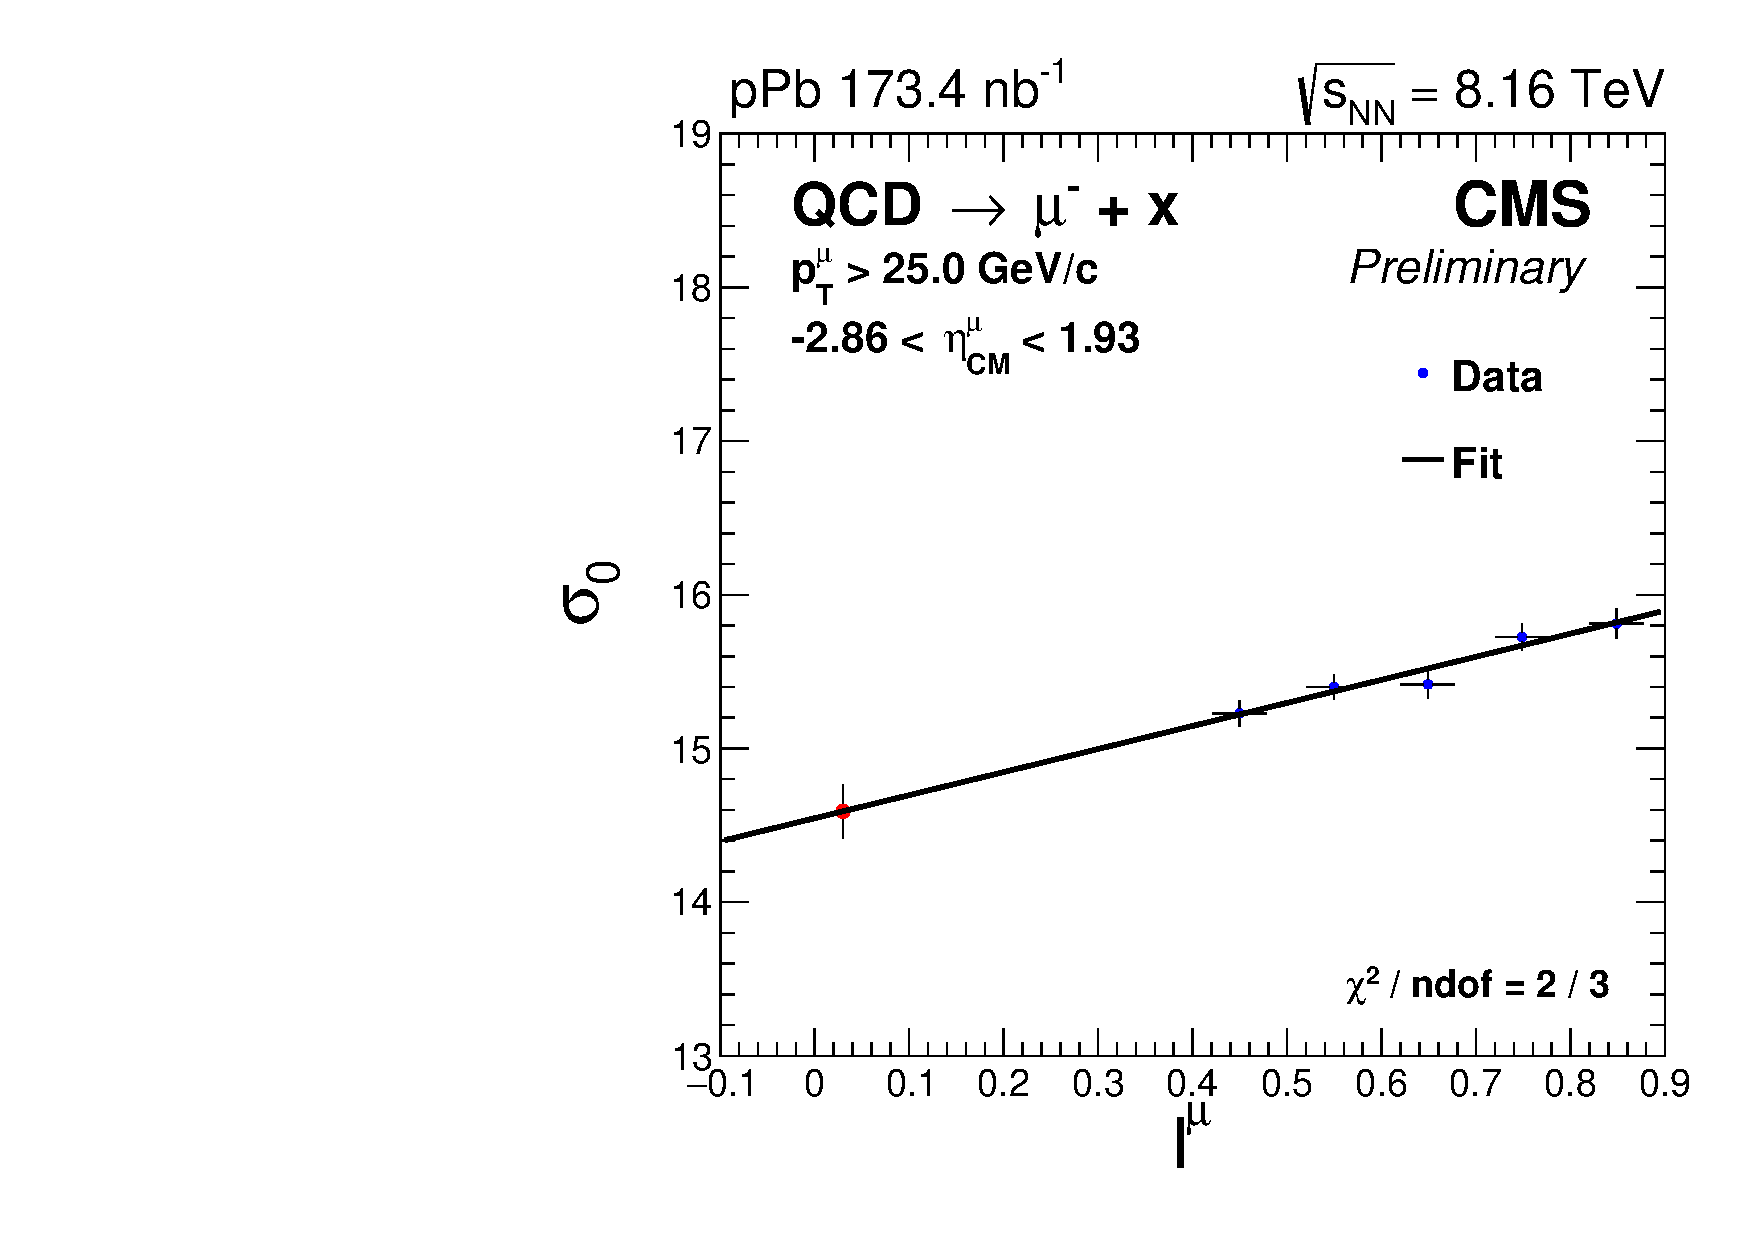
\includegraphics[width=0.32\textwidth]{Figures/WBoson/Analysis/SignalExtraction/QCD_Template/EXTRAPOLATION/graph_Sigma0_QCDToMuMi_PA_-29_eta_19_250_pt_1000000.pdf}
 \includegraphics[width=0.32\textwidth]{Figures/WBoson/Analysis/SignalExtraction/QCD_Template/EXTRAPOLATION/graph_Sigma1_QCDToMuMi_PA_-29_eta_19_250_pt_1000000.pdf}
 \includegraphics[width=0.32\textwidth]{Figures/WBoson/Analysis/SignalExtraction/QCD_Template/EXTRAPOLATION/graph_Sigma2_QCDToMuMi_PA_-29_eta_19_250_pt_1000000.pdf}
%%
 \includegraphics[width=0.32\textwidth]{Figures/WBoson/Analysis/SignalExtraction/QCD_Template/EXTRAPOLATION/graph_Sigma0_QCDToMuPl_PA_-29_eta_19_250_pt_1000000.pdf}
 \includegraphics[width=0.32\textwidth]{Figures/WBoson/Analysis/SignalExtraction/QCD_Template/EXTRAPOLATION/graph_Sigma1_QCDToMuPl_PA_-29_eta_19_250_pt_1000000.pdf}
 \includegraphics[width=0.32\textwidth]{Figures/WBoson/Analysis/SignalExtraction/QCD_Template/EXTRAPOLATION/graph_Sigma2_QCDToMuPl_PA_-29_eta_19_250_pt_1000000.pdf}
 \caption{Linear fits to the profile of the QCD background parameters: $\sigma_{0}$ (left), $\sigma_{1}$ (middle) and $\sigma_{2}$ (right), with respect to the muon isolation variable \iso. The results are shown for negative (top) and positive (bottom) charged muons in the \etaMuCM-inclusive range. The red points represents the value obtained by linearly extrapolating to $\iso = 0.03$.}
 \label{fig:QCD_Extrapolation}
\end{figure}

The $\sigma_{0}$, $\sigma_{1}$, and $\sigma_{2}$ parameters are extrapolated to the signal region (average muon isolation of 0.03) using the parametrisation as a function of \iso extracted from the linear fits. The values of the QCD background parameters derived from the extrapolation are presented in \tab{tab:QCD_Extrapolation}.

\begin{table}[htb!]
 \centering
 \begin{tabular}{|c|c|c|}\hline
   Parameter & $\text{QCD jet} \to \mu^{-}$ & $\text{QCD jet} \to \mu^{+}$ \\\hline
   $\sigma_{0}$ & 14.6$\pm$0.2 & 14.7$\pm$0.2 \\\hline
   $\sigma_{1}$ & 6.3$\pm$0.2 & 6.8$\pm$0.2 \\\hline
   $\sigma_{2}$ & 0.5$\pm$0.2 & 0.5$\pm$0.1 \\\hline
 \end{tabular}
 \caption{QCD background parameters extrapolated to $\iso = 0.03$. The results are presented for positive and negative charged muons in the \etaMuCM-inclusive range.}
 \label{tab:QCD_Extrapolation}
\end{table}

The dependence of the extrapolated QCD jet shape on the muon \etaMuCM is checked by splitting the control sample in different \etaMuCM bins, and then repeating the QCD jet shape extraction procedure for each \etaMuCM bin. The results of the extrapolated values of $\sigma_{0}$, $\sigma_{1}$, and $\sigma_{2}$, determined for each \etaMuCM bin, are compared in \fig{fig:QCD_Extrapolation_Eta} to the results obtained in the \etaMuCM-inclusive range.

\begin{figure}[htb!]
 \centering
  \includegraphics[width=0.32\textwidth]{Figures/WBoson/Analysis/SignalExtraction/QCD_Template/EXTRAPOLATION_ETA/exGraph_ETA_Sigma0_QCDToMuMi_PA.pdf}
  \includegraphics[width=0.32\textwidth]{Figures/WBoson/Analysis/SignalExtraction/QCD_Template/EXTRAPOLATION_ETA/exGraph_ETA_Sigma1_QCDToMuMi_PA.pdf}
  \includegraphics[width=0.32\textwidth]{Figures/WBoson/Analysis/SignalExtraction/QCD_Template/EXTRAPOLATION_ETA/exGraph_ETA_Sigma2_QCDToMuMi_PA.pdf}
%%
  \includegraphics[width=0.32\textwidth]{Figures/WBoson/Analysis/SignalExtraction/QCD_Template/EXTRAPOLATION_ETA/exGraph_ETA_Sigma0_QCDToMuPl_PA.pdf}
  \includegraphics[width=0.32\textwidth]{Figures/WBoson/Analysis/SignalExtraction/QCD_Template/EXTRAPOLATION_ETA/exGraph_ETA_Sigma1_QCDToMuPl_PA.pdf}
  \includegraphics[width=0.32\textwidth]{Figures/WBoson/Analysis/SignalExtraction/QCD_Template/EXTRAPOLATION_ETA/exGraph_ETA_Sigma2_QCDToMuPl_PA.pdf}
 \caption{Muon $\etaMuCM$ dependence of $\sigma_{0}$ (left), $\sigma_{1}$ (middle) and $\sigma_{2}$ (right) parameters extrapolated to $\iso = 0.03$. The results are shown for negative (top) and positive (bottom) charged muons. The red line corresponds to the QCD jet parameter extrapolated in the \etaMuCM-inclusive range.}
 \label{fig:QCD_Extrapolation_Eta}
\end{figure}

It is observed that the $\sigma_{0}$, $\sigma_{1}$, and $\sigma_{2}$ parameters, extrapolated to low muon isolation, do not vary significantly with respect to \etaMuCM and are found to be consistent with the corresponding values obtained in the \etaMuCM-inclusive range. As a result, the extrapolated parameters derived in the \etaMuCM-inclusive range for $\mu^{+}$ and $\mu^{-}$, are used to fix the QCD jet background shape when fitting the signal.


\subsubsection{Modelling of the signal, \ttbar and electroweak backgrounds}\label{sec:WBoson_Analysis_SignalExtraction_EWKBackground}

The \ptmiss  distribution of the signal, as well as, the \ttbar and electroweak background events, are estimated using the corresponding \POWHEG simulations mentioned in \sect{sec:WBoson_Analysis_Sample_MC}. The simulated events for each process are required to satisfy the signal selection criteria summarised in \sect{sec:WBoson_Analysis_Selection_WSelection}.

In order to improve the description of the data, several corrections are applied to the simulations. First, the simulated HF energy distribution is weighed as explained in \sect{sec:WBoson_Analysis_Corrections_EventActivityReweighing}. Then, the generated weak boson \pt distribution from the \WToMuNu, \WToTauNu, \DYToMuMu and \DYToTauTau simulations, is weighed as described in \sect{sec:WBoson_Analysis_Corrections_WeakBosonPTReweighing} And finally, the recoil of \WToMuNu, \WToTauNu and \DYToMuMu events is calibrated as detailed in \sect{sec:WBoson_Analysis_Corrections_RecoilCalib}, improving the agreement of the \ptmiss distribution between data and simulation.

Once the simulations have been corrected, the \ptmiss shape of the signal, \ttbar background and electroweak background, is determined by building a template histogram of the simulated \ptmiss distribution (2~\GeVc bin width). These template histograms are then used in the fitting procedure describe in the next section.


\subsubsection{Fit model}\label{sec:WBoson_Analysis_SignalExtraction_FitModel}

The number of \WToMuNu signal events is obtained by performing an unbinned maximum-likelihood fit of the observed \ptmiss distribution in different muon \etaMuCM regions. The fits are done using a combination of template histograms and a functional form. The data analysis framework RooFit v3.60~\cite{RooFit} is used to make the fits.

The total fit model includes six contributions: the signal \WToMuNu template ($\euscr{T}_{\Wb}$), the electroweak background templates \DYToMuMu ($\euscr{T}_{\DYToMu}$), \WToTauNu ($\euscr{T}_{\WToTau}$) and \DYToTauTau ($\euscr{T}_{\DYToTau}$), the \ttbar background template ($\euscr{T}_{\ttbar}$), and the QCD jet background functional form ($\euscr{F}_{\QCD}$). The model used to fit the data is:

\begin{equation}
   N_{\Wb} \cdot \left( {\euscr{T}_{\Wb}} + {r_{\DYToMu} \cdot \euscr{T}_{\DYToMu}} + {r_{\WToTau} \cdot \euscr{T}_{\WToTau}} + {r_{\DYToTau} \cdot \euscr{T}_{\DYToTau}} + {r_{\ttbar} \cdot \euscr{T}_{\ttbar}} \right) + { N_{\QCD} \cdot \euscr{F}_{\QCD} }
 \label{eq:FitModel}
\end{equation}

where $N_{\Wb}$ and $N_{\QCD}$ are the normalisation factors of the \WToMuNu signal and QCD jet background, $r_{\ttbar}$ represents the ratio of \ttbar background events over the number of signal events ($N_{\ttbar}\big/N_{\Wb}$), and 
$r_{\DYToMu}$, $r_{\DYToTau}$ and $r_{\WToTau}$ are the corresponding ratios for the \DYToMuMu, \DYToTauTau and \WToTauNu background processes, respectively.

The shapes of the signal, \ttbar background and electroweak background processes are defined based on template histograms extracted from simulations. Being very small and with a moderately discriminating shape, the  electroweak and \ttbar background components cannot be directly and independently fitted on data. Instead, we take advantage that their nuclear modification should be small and close to the one of the \Wb-boson signal. Thus, the ratios of \DYToMuMu, \DYToTauTau, \WToTauNu and \ttbar events over the number of \WToMuNu events, are fixed to the results from simulations after having normalised all the MC samples to the recorded integrated luminosity of data as detailed in \sect{sec:WBoson_Analysis_Sample_MC} and applied all analysis corrections and selection criteria.

The QCD jet background contribution is taken into account by means of a functional form depending on three parameters. For the fits to the \ptmiss distribution in the signal region, the $\sigma_{0}$ , $\sigma_{1}$ and $\sigma_{2}$ parameters are fixed to the extrapolated values mentioned in \tab{tab:QCD_Extrapolation}, and the normalisation is left free.

The \ptmiss distribution is fitted separately for \WToMuNuPl and \WToMuNuMi events. Only the signal ($N_{\Wb}$) and the QCD jet background ($N_{\QCD}$) normalisation factors are left free when fitting the signal region in data. The fits are done in the \etaMuCM-inclusive range and in bins of muon \etaMuCM. The results of the fits performed in the \etaMuCM-inclusive range are shown in \fig{fig:SignalFit} and those performed in the other muon \etaMuCM bins are presented in \app{app:WBoson_SignalExtraction_Fits}.

\begin{figure}[htb!]
 \centering
 \includegraphics[width=0.45\textwidth]{Figures/WBoson/Analysis/SignalExtraction/Signal/LIN/PLOT_MET_DATA_WToMuMi_PA_Model_TEMP_WDYDYToTauWToTauTTbar_ModifiedRayleigh_QCD_MuEtaCM_-286_193_MuIso_0_15.pdf}
%%
 \includegraphics[width=0.45\textwidth]{Figures/WBoson/Analysis/SignalExtraction/Signal/LIN/PLOT_MET_DATA_WToMuPl_PA_Model_TEMP_WDYDYToTauWToTauTTbar_ModifiedRayleigh_QCD_MuEtaCM_-286_193_MuIso_0_15.pdf}
 \caption{The \ptmiss distribution for \WToMuNuMi (left) and  \WToMuNuPl (right) events within the \etaMuCM-inclusive range, shown in linear scale. Unbinned fits to the data (black points) are performed with six contributions, stacked from top to bottom: \WToMuNu (yellow), QCD jet (light blue), \DYToMuMu (green), \WToTauNu (red), \DYToTauTau (dark blue) and \ttbar (orange). The lower panel, on each figure, display the ratio of the measurements over the result of the fit. The $\chi^{2}$ test value over the number of degrees of freedom is also shown.}
 \label{fig:SignalFit}
\end{figure}

\subsubsection{Extracted event yields}\label{sec:WBoson_Analysis_SignalExtraction_RawYields}

The results of the fits to the data in each of the different muon \etaCM bins are summarized in \tab{tab:RawYields_WToMuMi_PA} and \tab{tab:RawYields_WToMuPl_PA} for \WToMuNuMi and \WToMuNuPl events, respectively.

\begin{table}[htb!]
  \centering
  \resizebox{\textwidth}{!}{
  %\renewcommand{\arraystretch}{1.5}
  \begin{tabular}{|c|*7c|}
    \hline
    $\etaMuCM$ Range & Total & Signal & \DYToMuMu & \WToTauNu & \DYToTauTau & \ttbar & QCD\\
    \hline\hline
    $-$2.86 , $-$2.60 & 5210 & $4041 \pm 65$ & $560 \pm 9$ & $135 \pm 2$ & $45 \pm 1$ & $3.1 \pm 0.1$ & $427 \pm 40$\\
    \hline
    $-$2.60 , $-$2.40 & 4308 & $3395 \pm 60$ & $461 \pm 8$ & $102 \pm 2$ & $36 \pm 1$ & $4.0 \pm 0.1$ & $310 \pm 37$\\
    \hline
    $-$2.40 , $-$2.20 & 4273 & $3276 \pm 59$ & $449 \pm 8$ & $100 \pm 2$ & $36 \pm 1$ & $5.9 \pm 0.1$ & $407 \pm 38$\\
    \hline
    $-$2.20 , $-$1.93 & 6423 & $4920 \pm 74$ & $654 \pm 10$ & $156 \pm 2$ & $62 \pm 1$ & $12.9 \pm 0.2$ & $617 \pm 48$\\
    \hline
    $-$1.93 , $-$1.80 & 3140 & $2419 \pm 52$ & $303 \pm 6$ & $79 \pm 2$ & $28 \pm 1$ & $8.4 \pm 0.2$ & $302 \pm 34$\\
    \hline
    $-$1.80 , $-$1.60 & 4822 & $3672 \pm 64$ & $435 \pm 8$ & $117 \pm 2$ & $45 \pm 1$ & $15.2 \pm 0.3$ & $537 \pm 43$\\
    \hline
    $-$1.60 , $-$1.40 & 4727 & $3631 \pm 64$ & $390 \pm 7$ & $117 \pm 2$ & $39 \pm 1$ & $18.8 \pm 0.3$ & $533 \pm 43$\\
    \hline
    $-$1.40 , $-$1.20 & 4521 & $3590 \pm 64$ & $340 \pm 6$ & $109 \pm 2$ & $45 \pm 1$ & $21.6 \pm 0.4$ & $416 \pm 40$\\
    \hline
    $-$1.20 , $-$1.00 & 4626 & $3666 \pm 65$ & $306 \pm 5$ & $118 \pm 2$ & $48 \pm 1$ & $25.2 \pm 0.4$ & $463 \pm 42$\\
    \hline
    $-$1.00 , $-$0.80 & 4722 & $3762 \pm 66$ & $277 \pm 5$ & $119 \pm 2$ & $45 \pm 1$ & $32 \pm 1$ & $488 \pm 43$\\
    \hline
    $-$0.80 , $-$0.60 & 4198 & $3425 \pm 63$ & $238 \pm 4$ & $102 \pm 2$ & $46 \pm 1$ & $32 \pm 1$ & $355 \pm 39$\\
    \hline
    $-$0.60 , $-$0.40 & 4648 & $3738 \pm 66$ & $245 \pm 4$ & $119 \pm 2$ & $54 \pm 1$ & $35 \pm 1$ & $456 \pm 43$\\
    \hline
    $-$0.40 , $-$0.20 & 4344 & $3478 \pm 64$ & $226 \pm 4$ & $111 \pm 2$ & $50 \pm 1$ & $36 \pm 1$ & $443 \pm 41$\\
    \hline
    $-$0.20 , $+$0.00 & 4474 & $3510 \pm 65$ & $260 \pm 5$ & $113 \pm 2$ & $43 \pm 1$ & $39 \pm 1$ & $509 \pm 43$\\
    \hline
    $+$0.00 , $+$0.20 & 4643 & $3654 \pm 65$ & $309 \pm 6$ & $114 \pm 2$ & $47 \pm 1$ & $42 \pm 1$ & $477 \pm 43$\\
    \hline
    $+$0.20 , $+$0.40 & 4638 & $3533 \pm 64$ & $335 \pm 6$ & $111 \pm 2$ & $50 \pm 1$ & $42 \pm 1$ & $567 \pm 44$\\
    \hline
    $+$0.40 , $+$0.60 & 4718 & $3528 \pm 63$ & $390 \pm 7$ & $114 \pm 2$ & $46 \pm 1$ & $39 \pm 1$ & $601 \pm 44$\\
    \hline
    $+$0.60 , $+$0.80 & 4552 & $3375 \pm 62$ & $446 \pm 8$ & $103 \pm 2$ & $48 \pm 1$ & $37 \pm 1$ & $544 \pm 43$\\
    \hline
    $+$0.80 , $+$1.00 & 4637 & $3325 \pm 61$ & $489 \pm 9$ & $103 \pm 2$ & $43 \pm 1$ & $37 \pm 1$ & $640 \pm 44$\\
    \hline
    $+$1.00 , $+$1.20 & 4612 & $3265 \pm 60$ & $539 \pm 10$ & $105 \pm 2$ & $45 \pm 1$ & $29 \pm 1$ & $630 \pm 44$\\
    \hline
    $+$1.20 , $+$1.40 & 4053 & $2769 \pm 55$ & $517 \pm 10$ & $78 \pm 2$ & $38 \pm 1$ & $23.8 \pm 0.5$ & $627 \pm 42$\\
    \hline
    $+$1.40 , $+$1.60 & 4251 & $2917 \pm 56$ & $620 \pm 12$ & $96 \pm 2$ & $39 \pm 1$ & $21.5 \pm 0.4$ & $557 \pm 42$\\
    \hline
    $+$1.60 , $+$1.80 & 3844 & $2506 \pm 51$ & $611 \pm 12$ & $78 \pm 2$ & $35 \pm 1$ & $15.4 \pm 0.3$ & $599 \pm 41$\\
    \hline
    $+$1.80 , $+$1.93 & 2640 & $1719 \pm 42$ & $439 \pm 11$ & $54 \pm 1$ & $22 \pm 1$ & $9.6 \pm 0.2$ & $397 \pm 33$\\
    \hline
  \end{tabular}
  }
  \caption{Event yields of \WToMuNuMi and background processes, extracted from the fits to the \ptmiss distribution in each muon $\etaMuCM$ region. All analysis selection criteria are applied including the muon $p_{T} > 25$~GeV/c. All uncertainties shown are statistical only.}
  \label{tab:RawYields_WToMuMi_PA}
\end{table}


\begin{table}[htb!]
  \centering
  \resizebox{\textwidth}{!}{
  %\renewcommand{\arraystretch}{1.5}
  \begin{tabular}{|c|*7c|}
    \hline
    $\etaMuCM$ Range & Total & Signal & \DYToMuMu & \WToTauNu & \DYToTauTau & \ttbar & QCD\\
    \hline\hline
    $-$2.86 , $-$2.60 & 4465 & $3358 \pm 59$ & $583 \pm 10$ & $67 \pm 1$ & $44 \pm 1$ & $3.3 \pm 0.1$ & $409 \pm 38$\\
    \hline
    $-$2.60 , $-$2.40 & 4234 & $3247 \pm 58$ & $526 \pm 9$ & $65 \pm 1$ & $35 \pm 1$ & $4.2 \pm 0.1$ & $358 \pm 36$\\
    \hline
    $-$2.40 , $-$2.20 & 4377 & $3351 \pm 60$ & $500 \pm 9$ & $61 \pm 1$ & $36 \pm 1$ & $6.5 \pm 0.1$ & $423 \pm 38$\\
    \hline
    $-$2.20 , $-$1.93 & 6847 & $5257 \pm 76$ & $714 \pm 10$ & $101 \pm 1$ & $53 \pm 1$ & $14.3 \pm 0.2$ & $706 \pm 49$\\
    \hline
    $-$1.93 , $-$1.80 & 3592 & $2762 \pm 55$ & $335 \pm 7$ & $56 \pm 1$ & $29 \pm 1$ & $8.5 \pm 0.2$ & $400 \pm 36$\\
    \hline
    $-$1.80 , $-$1.60 & 5421 & $4299 \pm 69$ & $488 \pm 8$ & $94 \pm 2$ & $50 \pm 1$ & $16.0 \pm 0.3$ & $471 \pm 43$\\
    \hline
    $-$1.60 , $-$1.40 & 5343 & $4375 \pm 70$ & $446 \pm 7$ & $96 \pm 2$ & $45 \pm 1$ & $18.0 \pm 0.3$ & $364 \pm 42$\\
    \hline
    $-$1.40 , $-$1.20 & 5129 & $4182 \pm 69$ & $375 \pm 6$ & $98 \pm 2$ & $41 \pm 1$ & $23.4 \pm 0.4$ & $405 \pm 43$\\
    \hline
    $-$1.20 , $-$1.00 & 5382 & $4465 \pm 72$ & $339 \pm 5$ & $100 \pm 2$ & $53 \pm 1$ & $28.3 \pm 0.5$ & $395 \pm 43$\\
    \hline
    $-$1.00 , $-$0.80 & 5467 & $4485 \pm 73$ & $306 \pm 5$ & $100 \pm 2$ & $50 \pm 1$ & $32 \pm 1$ & $491 \pm 45$\\
    \hline
    $-$0.80 , $-$0.60 & 4738 & $3960 \pm 68$ & $244 \pm 4$ & $89 \pm 2$ & $42 \pm 1$ & $29 \pm 1$ & $373 \pm 41$\\
    \hline
    $-$0.60 , $-$0.40 & 5349 & $4435 \pm 73$ & $255 \pm 4$ & $99 \pm 2$ & $49 \pm 1$ & $38 \pm 1$ & $473 \pm 45$\\
    \hline
    $-$0.40 , $-$0.20 & 5027 & $4146 \pm 70$ & $238 \pm 4$ & $88 \pm 1$ & $46 \pm 1$ & $37 \pm 1$ & $468 \pm 43$\\
    \hline
    $-$0.20 , $+$0.00 & 5161 & $4269 \pm 71$ & $268 \pm 4$ & $99 \pm 2$ & $45 \pm 1$ & $39 \pm 1$ & $439 \pm 43$\\
    \hline
    $+$0.00 , $+$0.20 & 5473 & $4352 \pm 72$ & $308 \pm 5$ & $100 \pm 2$ & $52 \pm 1$ & $39 \pm 1$ & $621 \pm 47$\\
    \hline
    $+$0.20 , $+$0.40 & 5175 & $4179 \pm 70$ & $337 \pm 6$ & $99 \pm 2$ & $48 \pm 1$ & $37 \pm 1$ & $475 \pm 44$\\
    \hline
    $+$0.40 , $+$0.60 & 5482 & $4334 \pm 71$ & $399 \pm 7$ & $93 \pm 2$ & $43 \pm 1$ & $36 \pm 1$ & $576 \pm 46$\\
    \hline
    $+$0.60 , $+$0.80 & 5722 & $4469 \pm 72$ & $469 \pm 8$ & $99 \pm 2$ & $51 \pm 1$ & $38 \pm 1$ & $595 \pm 47$\\
    \hline
    $+$0.80 , $+$1.00 & 6061 & $4652 \pm 72$ & $561 \pm 9$ & $99 \pm 2$ & $48 \pm 1$ & $37 \pm 1$ & $664 \pm 48$\\
    \hline
    $+$1.00 , $+$1.20 & 5814 & $4404 \pm 70$ & $595 \pm 9$ & $102 \pm 2$ & $41 \pm 1$ & $33 \pm 1$ & $639 \pm 47$\\
    \hline
    $+$1.20 , $+$1.40 & 5365 & $4050 \pm 67$ & $570 \pm 9$ & $87 \pm 1$ & $35 \pm 1$ & $23.9 \pm 0.4$ & $596 \pm 45$\\
    \hline
    $+$1.40 , $+$1.60 & 5768 & $4308 \pm 68$ & $674 \pm 11$ & $92 \pm 1$ & $39 \pm 1$ & $21.5 \pm 0.3$ & $633 \pm 46$\\
    \hline
    $+$1.60 , $+$1.80 & 5320 & $3969 \pm 65$ & $662 \pm 11$ & $81 \pm 1$ & $34 \pm 1$ & $16.1 \pm 0.3$ & $557 \pm 44$\\
    \hline
    $+$1.80 , $+$1.93 & 3600 & $2654 \pm 53$ & $450 \pm 9$ & $63 \pm 1$ & $19.8 \pm 0.4$ & $9.3 \pm 0.2$ & $404 \pm 36$\\
    \hline
  \end{tabular}
  }
  \caption{Event yields of \WToMuNuPl and background processes, extracted from the fits to the \ptmiss distribution in each muon $\etaMuCM$ region. All analysis selection criteria are applied including the muon $p_{T} > 25$~GeV/c. All uncertainties shown are statistical only.}
  \label{tab:RawYields_WToMuPl_PA}
\end{table}




\subsubsection{Corrected event yields}\label{sec:WBoson_Analysis_SignalExtraction_CorrectedYields}

The signal event yields extracted from the fits are corrected by taking into account the efficiency of the detector, according to:

\begin{equation}
 N^{\pm}_{\mu}\left(\etaMuCM\right) = \frac{N^{\pm}_{\mu,\text{raw}}\left(\etaMuCM\right)}{\epsilon^{\pm}_{\corr}\left(\etaMuCM\right)}
 \label{eq:CorrectedYield}
\end{equation}

where $N_{\mu,\text{raw}}$ is the number of signal events extracted from the fits, $N_{\mu}$ is the number of signal events after correcting for efficiency and $\epsilon_{\corr}^{\pm}$ is the signal efficiency corrected with the TnP corrections. The statistical uncertainty of the corrected signal yields are computed based on error propagation with:

\begin{equation}
 \delta{N^{\pm}_{\mu}} = \frac{\delta{N^{\pm}_{\mu,\text{raw}}}\left(\etaMuCM\right)}{\epsilon^{\pm}_{\corr}\left(\etaMuCM\right)}
\label{eq:CorrectedYieldStatError}
\end{equation}

where $\delta{N^{\pm}_{\mu,\text{raw}}}$ is the uncertainty of the signal event yield determined from the fits to the data. The results of the corrected signal event yields for each muon \etaMuCM range are summarized in \tab{tab:CorrYields_WToMuMi_PA} and \tab{tab:CorrYields_WToMuPl_PA} for \WToMuNuMi and \WToMuNuPl events, accordingly.

\begin{table}[htb!]
  \centering
  %\renewcommand{\arraystretch}{1.5}
  \begin{tabular}{|c|*3c|}
    \hline
    $\etaMuCM$ Range & Extracted yield & Efficiency ($\%$) & Corrected yield\\
    \hline\hline
    $-$2.86 , $-$2.60 & $4041 \pm 65$ & $84.7 \pm 0.2$ & $4773 \pm 77$\\
    \hline
    $-$2.60 , $-$2.40 & $3395 \pm 60$ & $87.3 \pm 0.2$ & $3891 \pm 69$\\
    \hline
    $-$2.40 , $-$2.20 & $3276 \pm 59$ & $83.8 \pm 0.2$ & $3907 \pm 71$\\
    \hline
    $-$2.20 , $-$1.93 & $4920 \pm 74$ & $87.6 \pm 0.2$ & $5619 \pm 84$\\
    \hline
    $-$1.93 , $-$1.80 & $2419 \pm 52$ & $92.1 \pm 0.2$ & $2627 \pm 56$\\
    \hline
    $-$1.80 , $-$1.60 & $3672 \pm 64$ & $92.0 \pm 0.1$ & $3990 \pm 70$\\
    \hline
    $-$1.60 , $-$1.40 & $3631 \pm 64$ & $88.7 \pm 0.2$ & $4093 \pm 72$\\
    \hline
    $-$1.40 , $-$1.20 & $3590 \pm 64$ & $85.5 \pm 0.2$ & $4200 \pm 75$\\
    \hline
    $-$1.20 , $-$1.00 & $3666 \pm 65$ & $89.4 \pm 0.2$ & $4102 \pm 73$\\
    \hline
    $-$1.00 , $-$0.80 & $3762 \pm 66$ & $89.7 \pm 0.2$ & $4195 \pm 74$\\
    \hline
    $-$0.80 , $-$0.60 & $3425 \pm 63$ & $81.1 \pm 0.2$ & $4222 \pm 78$\\
    \hline
    $-$0.60 , $-$0.40 & $3738 \pm 66$ & $88.7 \pm 0.2$ & $4216 \pm 75$\\
    \hline
    $-$0.40 , $-$0.20 & $3478 \pm 64$ & $83.8 \pm 0.2$ & $4148 \pm 76$\\
    \hline
    $-$0.20 , $+$0.00 & $3510 \pm 65$ & $87.5 \pm 0.2$ & $4012 \pm 74$\\
    \hline
    $+$0.00 , $+$0.20 & $3654 \pm 65$ & $89.3 \pm 0.2$ & $4091 \pm 73$\\
    \hline
    $+$0.20 , $+$0.40 & $3533 \pm 64$ & $85.8 \pm 0.2$ & $4116 \pm 74$\\
    \hline
    $+$0.40 , $+$0.60 & $3528 \pm 63$ & $88.2 \pm 0.2$ & $4000 \pm 72$\\
    \hline
    $+$0.60 , $+$0.80 & $3375 \pm 62$ & $90.5 \pm 0.2$ & $3729 \pm 68$\\
    \hline
    $+$0.80 , $+$1.00 & $3325 \pm 61$ & $92.1 \pm 0.2$ & $3610 \pm 66$\\
    \hline
    $+$1.00 , $+$1.20 & $3265 \pm 60$ & $88.2 \pm 0.2$ & $3704 \pm 68$\\
    \hline
    $+$1.20 , $+$1.40 & $2769 \pm 55$ & $83.5 \pm 0.2$ & $3318 \pm 65$\\
    \hline
    $+$1.40 , $+$1.60 & $2917 \pm 56$ & $90.6 \pm 0.2$ & $3219 \pm 61$\\
    \hline
    $+$1.60 , $+$1.80 & $2506 \pm 51$ & $83.4 \pm 0.2$ & $3005 \pm 61$\\
    \hline
    $+$1.80 , $+$1.93 & $1719 \pm 42$ & $86.4 \pm 0.3$ & $1990 \pm 48$\\
    \hline
  \end{tabular}
  \caption{Corrected event yields of \WToMuNuMi, given for each muon $\etaMuCM$ bin. All analysis selection criteria are applied including the muon $p_{T} > 25$~GeV/c. The muon efficiency has been corrected by applying the tag-and-probe corrections, HF energy weights and vector boson \pt weights, event by event. All uncertainties shown are statistical only.}
  \label{tab:CorrYields_WToMuMi_PA}
\end{table}


\begin{table}[htb!]
  \centering
  %\renewcommand{\arraystretch}{1.5}
  \begin{tabular}{|c|*3c|}
    \hline
    $\etaMuCM$ Range & Extracted yield & Efficiency ($\%$) & Corrected yield\\
    \hline\hline
    $-$2.86 , $-$2.60 & $3358 \pm 59$ & $84.3 \pm 0.2$ & $3982 \pm 70$\\
    \hline
    $-$2.60 , $-$2.40 & $3247 \pm 58$ & $87.3 \pm 0.2$ & $3721 \pm 66$\\
    \hline
    $-$2.40 , $-$2.20 & $3351 \pm 60$ & $83.8 \pm 0.2$ & $3997 \pm 71$\\
    \hline
    $-$2.20 , $-$1.93 & $5257 \pm 76$ & $86.8 \pm 0.2$ & $6055 \pm 87$\\
    \hline
    $-$1.93 , $-$1.80 & $2762 \pm 55$ & $92.0 \pm 0.2$ & $3001 \pm 60$\\
    \hline
    $-$1.80 , $-$1.60 & $4299 \pm 69$ & $91.9 \pm 0.1$ & $4679 \pm 75$\\
    \hline
    $-$1.60 , $-$1.40 & $4375 \pm 70$ & $88.7 \pm 0.2$ & $4931 \pm 79$\\
    \hline
    $-$1.40 , $-$1.20 & $4182 \pm 69$ & $84.7 \pm 0.2$ & $4940 \pm 82$\\
    \hline
    $-$1.20 , $-$1.00 & $4465 \pm 72$ & $88.4 \pm 0.2$ & $5049 \pm 81$\\
    \hline
    $-$1.00 , $-$0.80 & $4485 \pm 73$ & $89.2 \pm 0.2$ & $5029 \pm 82$\\
    \hline
    $-$0.80 , $-$0.60 & $3960 \pm 68$ & $80.7 \pm 0.2$ & $4908 \pm 85$\\
    \hline
    $-$0.60 , $-$0.40 & $4435 \pm 73$ & $88.5 \pm 0.2$ & $5015 \pm 83$\\
    \hline
    $-$0.40 , $-$0.20 & $4146 \pm 70$ & $83.0 \pm 0.2$ & $4996 \pm 85$\\
    \hline
    $-$0.20 , $+$0.00 & $4269 \pm 71$ & $87.2 \pm 0.2$ & $4897 \pm 81$\\
    \hline
    $+$0.00 , $+$0.20 & $4352 \pm 72$ & $89.2 \pm 0.2$ & $4881 \pm 81$\\
    \hline
    $+$0.20 , $+$0.40 & $4179 \pm 70$ & $85.0 \pm 0.2$ & $4915 \pm 82$\\
    \hline
    $+$0.40 , $+$0.60 & $4334 \pm 71$ & $88.3 \pm 0.2$ & $4908 \pm 81$\\
    \hline
    $+$0.60 , $+$0.80 & $4469 \pm 72$ & $90.4 \pm 0.2$ & $4944 \pm 79$\\
    \hline
    $+$0.80 , $+$1.00 & $4652 \pm 72$ & $91.6 \pm 0.2$ & $5081 \pm 79$\\
    \hline
    $+$1.00 , $+$1.20 & $4404 \pm 70$ & $87.8 \pm 0.2$ & $5016 \pm 80$\\
    \hline
    $+$1.20 , $+$1.40 & $4050 \pm 67$ & $83.2 \pm 0.2$ & $4867 \pm 80$\\
    \hline
    $+$1.40 , $+$1.60 & $4308 \pm 68$ & $90.3 \pm 0.2$ & $4773 \pm 76$\\
    \hline
    $+$1.60 , $+$1.80 & $3969 \pm 65$ & $83.1 \pm 0.2$ & $4776 \pm 78$\\
    \hline
    $+$1.80 , $+$1.93 & $2654 \pm 53$ & $86.9 \pm 0.2$ & $3054 \pm 61$\\
    \hline
  \end{tabular}
  \caption{Corrected event yields of \WToMuNuPl, given for each muon $\etaMuCM$. All analysis selection criteria are applied including the muon $p_{T} > 25$~GeV/c. The muon efficiency has been corrected by applying the tag-and-probe corrections, HF energy weights and vector boson \pt weights, event by event. All uncertainties shown are statistical only.}
  \label{tab:CorrYields_WToMuPl_PA}
\end{table}






% END OF SUBSECTION

\subsection{Observables} \label{sec:WBoson_Analysis_Observables}

The main motivation behind measuring the \Wb-boson production in \RunpPb collisions is to probe the nuclear modifications of the PDFs. To accomplish this, the efficiency-corrected \WToMuNu event yields are combined to measure three kinds of observables: cross sections, muon charge asymmetry and forward-backward ratios.

\paragraph{\WToMuNu cross sections.} The \WToMuNupm differential cross sections are computed as a function of \etaMuCM, according to:

\begin{equation}
 \frac{\dd\sigma{(\WToMuNupm)}}{\dd\etaMuCM}\left(\etaMuCM\right) = \frac{N^{\pm}_{\PGm}\left(\etaMuCM\right)}{\Lumi \cdot \Delta{\etaMuCM}}
 \label{eq:CrossSection}
\end{equation}

where $\Lumi = 173.4{\pm}6.1$~\nbinv is the recorded integrated luminosity, $\Delta\etaMuCM$ is the width of the \etaMuCM range in which the measurement is performed and $N_{\PGm}\left(\etaMuCM\right)$ is the number of signal events after correcting for efficiency.

\paragraph{Muon charge asymmetry.} The muon charge asymmetry measures the difference between the event yields of the \WToMuNuMi and \WToMuNuPl processes, which is sensitive to the number of protons and neutrons in the nucleus (isospin effect), and to the flavour dependence of the nuclear modifications of the PDFs. It is defined in the following way:

\begin{equation}
 \ChgAsym\left(\etaMuCM\right) = \frac{N_{\PGm}^{+}\left(\etaMuCM\right) - N_{\PGm}^{-}\left(\etaMuCM\right)}{N_{\PGm}^{+}\left(\etaMuCM\right) + N_{\PGm}^{-}\left(\etaMuCM\right)}
 \label{eq:MuonChargeAsymmetry}
\end{equation}

where $N_{\PGm}^{-}$ and $N_{\PGm}^{+}$ represents the efficiency-corrected number of \WToMuNuMi and \WToMuNuPl events, respectively.

\paragraph{Forward-backward ratios.} To probe the modification of the PDFs between different pseudorapidity regions, the signal event yields  measured in the forward region ($\etaMuCM > 0$) are combined with those measured in the backward region ($\etaMuCM < 0$), to derive forward-backward ratios. These ratios are computed separately for \WToMuNuPl and \WToMuNuMi events in the following way:

\begin{equation}
 \RFBpm\left(\etaMuCM\right) = \frac{ N^{\pm}_{\PGm}\left(+\etaMuCM\right) }{ N^{\pm}_{\PGm}\left(-\etaMuCM\right) }
 \label{eq:MuonForwardBackwardAsymmetryCharged}
\end{equation}

A forward-backward ratio is also derived for all \WToMuNu events, by combining the yields of the \WToMuNuMi and \WToMuNuPl processes, according to:

\begin{equation}
 \RFB\left(\etaMuCM\right) = \frac{ N^{+}_{\PGm}\left(+\etaMuCM\right) + N^{-}_{\PGm}\left(+\etaMuCM\right) }{ N^{+}_{\PGm}\left(-\etaMuCM\right) + N^{-}_{\PGm}\left(-\etaMuCM\right) }
 \label{eq:MuonForwardBackwardAsymmetry}
\end{equation}

% END OF SUBSECTION

\subsection{Systematic uncertainties}\label{sec:WBoson_Analysis_Systematics}

This section presents the different sources and the procedure employed to determine the systematic uncertainties in the measurement of the \Wb-boson production in \RunpPb collisions. 

%%------------------------------------------------------------%%
\subsubsection{Luminosity}

The recorded integrated luminosity of the 2016 \RunpPb data sample is 173.4~\nbinv, and is known with a precision of 3.5\%~\cite{LUM-17-002}. Since the integrated luminosity cancels in forward-backward ratios and in the muon charge asymmetry, it only affects the measurement of the \WToMuNu differential cross sections. In this case, this 3.5\% systematic uncertainty is global and the bin-to-bin correlations is 100\%. This uncertainty is the dominant one on the \WToMuNu differential cross sections.


%%------------------------------------------------------------%%
\subsubsection{Signal efficiency}

The dominant systematic uncertainty on the forward-backward ratios and muon charge asymmetry are due to the estimation of the signal efficiency. Since the signal efficiencies are computed from simulations and corrected using the TnP corrections, two sources of systematic uncertainties are considered. The first one corresponds to the theoretical modelling of the simulated signal, which takes into account the uncertainty on the nuclear PDFs and the impact of the renormalisation and factorisation scales. The second source corresponds to the TnP correction uncertainties, which derives from the \ZToMuMu control sample used to extract the TnP data efficiencies.

\paragraph{Theoretical modelling.} The NLO model used to generate the simulations can impact the measurement of the signal efficiencies. The main sources of theoretical uncertainties include the choice of the nuclear parton distribution function (EPPS16+CT14), and the renormalisation and factorisation scales.

Since the PDFs are not calculable from first principles but are determined experimentally, in particular by the measurements reported here, the inclusion of any PDF introduces an additional systematic uncertainty. Thus, it is important to determine the impact of a change of PDF on the signal efficiencies. The procedure to derive the theoretical uncertainties of the PDF variations consist of reweighing the simulations event-by-event using weights derived from \POWHEG after applying various PDF sets. The PDF sets are accessed through the LHAPDF6~\cite{LHAPDF6} framework and consist of 56 CT14 PDFs and 40 EPPS16 nuclear corrections. Once the simulations are reweighed with each PDF set, the efficiencies are recomputed and used to recalculate all the observables. The nPDF uncertainty is determined by combining the EPPS16+CT14 PDF variations of the observables using the Hessian approach, as recommended by the EPPS16 authors~\cite{EPPS16}. 

Moreover, the uncertainty due to the renormalisation ($\mu_{R}$) and factorisation ($\mu_{F}$) scales is computed by varying these two scales in \POWHEG using the following six combinations:
\begin{equation*}
(\mu_{R} , \mu_{F}) = [\ (0.5 , 0.5)\ ,\ (1.0 , 0.5)\ ,\ (0.5 , 1.0)\ ,\ (1.0 , 2.0)\ ,\ (2.0 , 1.0)\ ,\ (2.0 , 2.0)\ ]
\end{equation*}

The simulations are reweighed event by event using the \POWHEG weights produced with each set of scales, then the efficiencies are recomputed and the observables are recalculated for each varied efficiency. The variations on the observables are combined by taking the envelope (i.e. the maximum variation in each \etaMuCM range).

The systematic uncertainties from the PDF and scale variations are summed in quadrature, and amount to 0.1\%. Thus, the theoretical uncertainties have negligible impact on the signal efficiencies.

\paragraph{Tag-and-probe correction.} The main source of systematic uncertainty in the measurement of the signal efficiency arises from the application of the TnP corrections. As mentioned in \sect{sec:WBoson_Analysis_Efficiency_Corrected}, the statistical and systematic uncertainties of the TnP corrections are derived from the muon identification, isolation and trigger efficiencies measured in data.

It is crucial to consider the correlation between the different TnP uncertainties as a function of muon pseudorapidity and its charge, since they could cancel in the forward-backward ratios and muon charge asymmetry. The statistical TnP variations are uncorrelated between the different \etaLAB ranges in which they were derived. The systematic TnP variations are considered to be fully correlated as a function of muon charge since the detector response is the same for muons and anti-muons, and uncorrelated between the different \etaCM ranges (spanning different detectors).

To compute the uncertainties, the muon charge asymmetry and the forward-backward ratios are recalculated for each efficiency derived by varying the TnP corrections. The TnP uncertainties are then determined by taking the difference between the value obtained with the varied TnP correction and its nominal value, combining the uncertainties as explained in \sect{sec:WBoson_Analysis_Efficiency_Corrected}. If the source of TnP correction is correlated in muon charge or pseudorapidity, the corresponding signal yields are varied at the same time. Moreover, for the \Wpm differential cross sections, the statistical and systematic TnP uncertainties are calculated by propagating the uncertainties on the corrected signal efficiency.

The systematic uncertainty due to the TnP corrections amounts to 3.2\% and the dominant TnP uncertainties  are derived from the TnP systematic variations of the muon isolation (2.5\%) and trigger (1.1\%) components.

%%------------------------------------------------------------%%
\subsubsection{QCD jet background}

The systematic uncertainty in the QCD jet background originates from the uncertainty in the modelling of the QCD jet \ptmiss distribution in the signal region. The nominal procedure consists in fixing the parameters of the modified Rayleigh distribution from the fits extrapolated from data as explained in \sect{sec:WBoson_Analysis_SignalExtraction_QCDBackground}. In order to estimate the uncertainty of the mismodelling of the QCD jet background shape, both the parameters and the functional form are varied.

\paragraph{QCD jet background parameters.} The first source of systematic uncertainty reflects the possible mismodelling of the QCD jet background shape due to the \etaMuCM dependence of the QCD background parameters. In order to check this, the parameters of the nominal QCD jet model are set free but constrained to be near their nominal values by using a Gaussian penalty. The width of the penalty Gaussian function is fixed, for a given QCD background parameter, to the root mean square (RMS) of the set of extrapolated results along all \etaMuCM ranges, shown in \fig{fig:QCD_Extrapolation_Eta}. The RMS values used in the Gaussian penalty for the $\sigma_{0}$,  $\sigma_{1}$ and  $\sigma_{2}$ parameters are presented in \tab{tab:QCDContrainPar}. The difference between the number of signal events extracted from the Gaussian-constrained fits and the nominal fits is taken as the systematic uncertainty, which is then propagated to all observables. This source of uncertainty is considered to be fully uncorrelated since the \ptmiss distribution in each \etaMuCM range is fitted separately.

\begin{table}[htb!]
  \centering
  \begin{tabular}{|c|c c|}\hline
  \multirow{2}{*}{Parameter} & \multicolumn{2}{|c|}{RMS} \\
   & $QCD \to \mu^{-}$ & $QCD \to \mu^{+}$ \\\hline
  $\sigma_{0}$ & 1.0 & 0.5 \\\hline
  $\sigma_{1}$ & 0.9 & 0.9\\\hline
  $\sigma_{2}$ & 0.7 & 0.6\\\hline
  \end{tabular}
  \caption{The RMS of the set of QCD background parameters extrapolated along all \etaMuCM regions.}
  \label{tab:QCDContrainPar}
\end{table}

Another systematic variation consists of changing the muon isolation point used to extrapolate the QCD background parameters. In the nominal case, the isolation point of 0.03 is determined from the average muon isolation value in data within the signal region. As an alternative case, the muon isolation distribution is checked in a QCD \PYTHIA simulated sample satisfying the signal selection criteria, and the average isolation value is determined to be approximately 0.08. As a result, the QCD background parameters are recomputed by extrapolating them to an isolation point of $\iso=0.08$, and the fits are redone by fixing the QCD background parameters to the extrapolated values in the \etaMuCM-inclusive range as in the nominal case. The difference between the number of signal events extracted from the fits using the varied QCD background shape and the nominal results is taken as the systematic uncertainty. This uncertainty is propagated to all observables. The QCD background parameters extrapolated to $\iso=0.08$ are listed in \tab{tab:QCDFixedPar_Iso0p08}. Since the result in each \etaMuCM range varies independently, the uncertainty is considered to be fully uncorrelated.

\begin{table}[htb!]
  \centering
  \begin{tabular}{|c|c|c|}\hline
   Parameter & $QCD \to \mu^{-}$ & $QCD \to \mu^{+}$ \\\hline
   $\sigma_{0}$ & 14.67 & 14.79 \\\hline
   $\sigma_{1}$ & 6.28 & 6.71 \\\hline
   $\sigma_{2}$ & 0.50 & 0.49 \\\hline
  \end{tabular}
  \caption{QCD shape parameters extrapolated to the average muon isolation point $\text{iso} = 0.08$.}
  \label{tab:QCDFixedPar_Iso0p08}
\end{table}

The systematic uncertainty associated to the \etaMuCM dependence of the QCD background parameters amounts to 1.1\%, while the uncertainty corresponding to the change of extrapolation point represents 0.2\%.

\paragraph{QCD jet background functional form.} To assign a systematic uncertainty due to the assumed functional form for modelling the QCD jet background \ptmiss distribution, the shape of the QCD jet background is described using a different model. The alternative \ptmiss functional form employed, taken from Ref.\cite{HIN-13-007}, is given by: 

\begin{equation}\label{eq:QCDMultiJet}
  f_{\text{QCD}}\left(\ptmiss\right) = \left(\ptmiss+x_0\right)^{\alpha}\cdot\exp\left(\beta\cdot\sqrt{\ptmiss+x_0}\right)
\end{equation}

The extrapolation procedure explained in \sect{sec:WBoson_Analysis_SignalExtraction_QCDBackground} is redone using the alternative model. All the fits are remade using the alternative QCD background functional form fixed to the parameters extrapolated in the \etaMuCM-inclusive range. The difference between the number of signal events measured using the alternative QCD background model and the nominal results is taken as the systematic uncertainty due to mismodelling of the QCD jet background shape. This systematic uncertainty is propagated to all observables and amounts to 0.6\%. The bin-to-bin correlation is taken to be fully uncorrelated.

%%------------------------------------------------------------%%
\subsubsection{Electroweak and \ttbar backgrounds}

The \ttbar background and the different sources of electroweak background are described using template histograms derived from simulations. The simulated samples are scaled to the recorded integrated luminosity of data using the NLO \POWHEG cross sections for the electroweak processes and the CMS measured cross section for the \ttbar production. Since for each these background sources, the ratio of background over signal events is fixed to simulation when performing the fits, a systematic uncertainty is assigned to each source by varying up and down their cross sections as explained below. The systematic uncertainty in each \etaMuCM range is derived by taking the maximum difference between the nominal and the up/down variations. The bin-to-bin correlations in muon charge and pseudorapidity are considered correlated since the total cross section is used to normalise all simulated events.

\paragraph{\texorpdfstring{\DYToMuMu}\ background.} The uncertainty on the ratio of $\Z/\Wb$ total cross sections is estimated using the Monte Carlo for FeMtobarn processes (MCFM) program~\cite{MCFM} at NLO with the CT14+EPPS16 nuclear PDFs. A relative uncertainty of $0.8\%$ for $Z/\Wm$ and $1.3\%$ for $Z/\Wp$ cross-section ratios is determined with MCFM taking into account the PDF uncertainties. Since the cross sections in the muon channel depend on the branching ratio associated to each process, their uncertainty has to also be taken into account. The values of the branching ratios correspond to $\textrm{BR}(\ZToMuMu) = (3.366 \pm 0.007)\%$ and $\textrm{BR}(\WToMuNu) = (10.63 \pm 0.15)\%$~\cite{PDG}, which gives a relative uncertainty on the ratio of $\Z/\Wb$ branching ratios of $1.4\%$. Summing in quadrature the MCFM uncertainties with the ones derived from the branching ratios, one gets a total relative uncertainty for $\Z/\Wp$ of $1.6\%$ and for $\Z/\Wm$ of $1.9\%$. To be conservative the systematic variation is fixed to $2\%$ overall. The systematic uncertainty is then determined by varying the \DYToMuMu cross section by $2\%$ up and down when performing the fits, yielding a change of 0.3\% in the measured \WToMuNu cross sections.

\paragraph{\texorpdfstring{\DYToTauTau}\ background.} The uncertainty on the ratio of \DYToTauTau background over signal events is considered to be the same as the 2\% uncertainty determined for the \DYToMuMu background. Hence, the \DYToTauTau cross section is varied by $2\%$ up and down when performing the fits. The impact of this systematic uncertainty is negligible and modifies the \WToMuNu cross sections by 0.01\%.

\paragraph{\texorpdfstring{\WToTauNu}\ background.} The values of the \Wb-boson leptonic branching ratios correspond to $\textrm{BR}(\WToMuNu) = (10.63 \pm 0.15)\%$ and $\textrm{BR}(\WToTauNu) = (11.38 \pm 0.21)\%$~\cite{PDG}, which gives a relative uncertainty on the ratio of \WToTauNu over \WToMuNu cross sections of $2.3\%$. Thus, the systematic uncertainty is estimated by varying the ratio of \WToTauNu to signal events up and down by $\pm$2.3\%. The impact of this systematic uncertainty on the \WToMuNu cross sections is found to be 0.04\%.

\paragraph{\texorpdfstring{\ttbar}\ background.} The \ttbar simulation is normalized using the CMS measured total cross section $\sigma_{\ttbar} = 45 \pm 8~\nbinv$~\cite{HIN-17-002}. The systematic related to the \ttbar background normalization is computed by varying up and down the \ttbar cross section by its measured relative uncertainty ($\pm$18\%). This systematic uncertainty amounts to 0.2\%.

%%------------------------------------------------------------%%
\subsubsection{Weak boson \pt}\label{sec:Systematic_BosonPTCorr}

The modelling of the weak boson \pt in the signal and electroweak background simulations is corrected by weighing event-by-event the generated weak boson \pt distribution following the procedure described in \sect{sec:WBoson_Analysis_Corrections_WeakBosonPTReweighing}. To determine the impact of the modelling of the weak boson \pt, the boson \pt corrections are removed and both the efficiency and the fits to the \ptmiss distribution are remade. The systematic uncertainty is determined in each \etaMuCM range from the difference between the nominal results and the results obtained without weighing the generated boson \pt distribution. This uncertainty amounts to 0.5\% and it is considered to be correlated with respect to muon charge and pseudorapidity.

%%------------------------------------------------------------%%
\subsubsection{Event activity}

The modelling of the event activity present in \RunpPb collisions is improved by weighing the distribution of the total HF energy, as explained in \sect{sec:WBoson_Analysis_Corrections_EventActivityReweighing}. The event activity is also correlated with other global variables, such as the number of tracks per event.
Since the pseudorapidity coverage of the tracker ($|\eta| < 2.5$) and the HF calorimeter ($3.0 < |\eta| < 5.4$) is different, the HF energy and the track multiplicity are sensitive to different kinematic regions of the event activity. Thus, the systematic uncertainty on the modelling of the event activity is determined by weighing instead the distribution of the simulated track multiplicity following the same procedure as the one used for the HF energy. The fits to the \ptmiss distribution and the signal efficiency are recomputed after weighing the simulated track multiplicity distribution. The difference between the varied and nominal observables is assigned as the systematic uncertainty in each muon \etaMuCM range. This uncertainty is considered correlated in muon charge and pseudorapidity, and it amounts to 0.6\%.

%%------------------------------------------------------------%%
\subsubsection{Recoil calibration}

The uncertainties due to the recoil calibration are of different nature: statistical and systematic. The statistical component arises from the uncertainties associated to the recoil scale and resolution derived from the fits to the recoil distributions from data. The systematic components arise from the following sources:
\begin{itemize}
 \item The recoil calibration method employed to correct the simulated \ptmiss distribution;
 \item The choice of functional form used to fit the recoil distributions in each \qtZ range;
 \item The parametrisation of the \qt dependence of the recoil scale and resolution.
\end{itemize}

\paragraph{Statistical component.} In order to estimate the uncertainty associated to the recoil resolution, the weighed average Gaussian widths of the perpendicular and parallel recoil components, defined in \eq{eq:SigmaAvg}, are randomly smeared in each \qtZ range using a Gaussian distribution centred on the parameter value and with a width equal to the parameter uncertainty. The \qt dependence is parametrised again using the nominal functions presented in \eq{eq:equreolnparam}. The procedure is repeated a hundred times, and the recoil calibrations are applied to the simulated \ptmiss distributions, redoing the measurements every time. The RMS of the number of signal events extracted from the fits using each variation of the recoil calibration, is used to determine the statistical uncertainty of the recoil calibration. This uncertainty is propagated to all observables and amounts to 0.09\%. It is considered fully uncorrelated.

\paragraph{Systematic components.} The fit function used to parametrise the \qt dependence of the recoil scale and resolution, is varied in both data and simulation to determine the associated uncertainty. Instead of using the nominal functions for the Gaussian mean (\eq{eq:equparparam}) and Gaussian widths (\eq{eq:equreolnparam}), a second order polynomial is used to parametrise the Gaussian parameters with respect to \qtZ. The varied recoil calibration is applied to the simulated \ptmiss distributions, which are then used to extract the signal from the data. The difference between the observables measured using the varied recoil calibration and the nominal observables, in each \etaMuCM, is assigned as a systematic uncertainty.

The uncertainty on the shape of the recoil distributions in each \qtZ range is estimated by varying the recoil fit model. Instead of using a sum of two Gaussian functions, the recoil distributions are parametrised with a sum of a Breit-Wigner and a Gaussian distribution, in both data and simulation (varied at the same time). The resulting \qt dependence of the recoil scale and resolution is determined following the nominal procedure and the measurements are performed again. The systematic uncertainty is determined as the variation between the observables derived with the varied recoil calibration and the nominal ones.

Moreover, the uncertainty associated to the method used to apply the recoil calibration is determined by smearing the recoil distributions as described in \eq{eq:RecoilCorrAlt}, instead of scaling them as done in the nominal case. The difference between the varied and nominal observables in each \etaMuCM is assigned as a systematic uncertainty.

The largest source of systematic uncertainty in this case is the one associated to the shape of the recoil distribution, which amounts to 0.3\%. The uncertainty related to the recoil calibration represents 0.2\%, while the uncertainty corresponding to the \qt dependence of the recoil scale and resolution is determined to be 0.06\%. These uncertainties are considered correlated both in muon charge and pseudorapidity.

%%------------------------------------------------------------%%
\subsubsection{W-boson POWHEG BOX}

The \WToMuNu simulations were generated using the \POWHEGBOX package \verb#W_ew-BMMNP#~\cite{POWHEGBOX_W_ew_BMNNP}, in which electroweak NLO corrections are implemented. In order to asses the impact of these NLO corrections on the final results, the \WToMuNu simulations were remade instead using the standard \POWHEGBOX package \verb#W#~\cite{POWHEGBOX_W}, which does not include electroweak NLO corrections, following the same procedure described in \sect{sec:WBoson_Analysis_Sample_MC}.

To determine the systematic uncertainty, the signal efficiencies and the template histograms for the signal were recomputed using the \WToMuNu simulations without electroweak NLO corrections. Then, the fits to the \ptmiss distribution in data were performed again, and the difference between the observables measured using the varied signal templates and the nominal results is assigned as a systematic uncertainty in each $\etaMuCM$ range. This uncertainty amounts to 0.9\% and it is considered to be fully correlated.

%%------------------------------------------------------------%%
\subsubsection{Summary of systematic uncertainties}

The largest systematic uncertainty for each category among all \etaMuCM ranges is summarised in \tab{tab:Systematics}. The systematic uncertainties are shown for each observable, including the \WToMuNu cross sections, muon charge asymmetry and the forward-backward ratios. The uncertainties presented for the cross sections are relative while those for the forward-backward ratios and the muon charge asymmetry are absolute.

\begin{table}[htb!]
  \centering
  \resizebox{\textwidth}{!}{
  %\renewcommand{\arraystretch}{1.5}
  \begin{tabular}{|c|*6c|}
    \hline
    Systematic Variation & $\sigma\left(\WToMuNuMi\right)$~[$\%$]  & $\sigma\left(\WToMuNuPl\right)$~[$\%$] & $\RFBm$ & $\RFBp$ & $\RFB$ & $\ChgAsym$\\
    \hline
    Luminosity &  3.5  &  3.5  &  0.000  &  0.000  &  0.000  &  0.000 \\
    \hline
    Signal efficiency &  3.0  &  3.2  &  0.026  &  0.037  &  0.030  &  0.011 \\
    \hline
    QCD jet background &  1.2  &  0.7  &  0.016  &  0.007  &  0.009  &  0.006 \\
    \hline
    Electroweak and \ttbar backgrounds &  0.4  &  0.3  &  0.002  &  0.001  &  0.001  &  0.000 \\
    \hline
    Weak boson \pt &  0.5  &  0.4  &  0.001  &  0.001  &  0.001  &  0.001 \\
    \hline
    Event activity &  0.6  &  0.4  &  0.002  &  0.002  &  0.001  &  0.002 \\
    \hline
    Recoil calibration &  0.2  &  0.3  &  0.002  &  0.004  &  0.002  &  0.002 \\
    \hline
    W-boson \POWHEGBOX &  0.9  &  0.5  &  0.007  &  0.004  &  0.006  &  0.003 \\
    \hline
    Total systematic uncertainty &  4.8  &  4.8  &  0.030  &  0.038  &  0.031  &  0.013 \\
    \hline
    Statistical  uncertainty &  2.4  &  2.0  &  0.026  &  0.029  &  0.019  &  0.015 \\
    \hline
  \end{tabular}
  }
  \caption{Maximum uncertainty of the measured observables determined for each category. The uncertainties of the \WToMuNu differential cross sections are relative while for the forward-backward ratios and muon charge asymmetry are absolute.}
  \label{tab:Systematics}
\end{table}




The uncertainties of the measurements are shown in \fig{fig:Summary_Systematics} as a function of \etaMuCM. They are observed to be similar between the different \etaMuCM ranges, except for the most backward and forward regions, which are driven by the systematic uncertainty on the signal efficiency. It is also seen that the systematic uncertainties dominates on the \WToMuNupm differential cross sections and the forward-backward ratios in all \etaMuCM ranges. In the case of the muon charge asymmetry, most of the systematic uncertainties are found to be suppressed due to the correlations in muon charge, and as a result, the statistical uncertainties dominates in most of the \etaMuCM ranges.


\begin{figure}[htb!]
 \centering
 \includegraphics[width=0.32\textwidth]{Figures/WBoson/Analysis/Systematics/gr_WToMuMi_PA_Cross_Section_EffTnP.pdf}
 \includegraphics[width=0.32\textwidth]{Figures/WBoson/Analysis/Systematics/gr_WToMuMi_PA_ForwardBackward_Ratio_EffTnP.pdf}
 \includegraphics[width=0.32\textwidth]{Figures/WBoson/Analysis/Systematics/gr_WToMuInc_PA_ForwardBackward_Ratio_EffTnP.pdf}
%%
 \includegraphics[width=0.32\textwidth]{Figures/WBoson/Analysis/Systematics/gr_WToMuPl_PA_Cross_Section_EffTnP.pdf}
 \includegraphics[width=0.32\textwidth]{Figures/WBoson/Analysis/Systematics/gr_WToMuPl_PA_ForwardBackward_Ratio_EffTnP.pdf}
 \includegraphics[width=0.32\textwidth]{Figures/WBoson/Analysis/Systematics/gr_WToMuInc_PA_Charge_Asymmetry_EffTnP.pdf}
 \caption{Uncertainty corresponding to each category as function of the muon \etaCM. The plots are divided as: \WToMuNuMi (top-left) and \WToMuNuPl (bottom-left) differential cross sections, \WToMuNuMi (top-middle) and \WToMuNuPl (bottom-middle) forward-backward ratios, and finally the charge-summed forward-backward ratio (top-right) and muon charge asymmetry (bottom-right). The uncertainties of the cross sections are relative while for the forward-backward ratios and muon charge asymmetry are absolute. The global luminosity uncertainty of 3.5\% is not included.}
 \label{fig:Summary_Systematics}
\end{figure}


%%------------------------------------------------------------%%
\subsubsection{Covariance matrix}\label{sec:WBoson_Analysis_Systematics_CovarianceMatrix}

The covariance matrices of the \WToMuNu differential cross sections, the forward-backward ratios and the muon charge asymmetry are computed by taking into account the measurements extracted in each \etaMuCM range. In the case of the \WToMuNupm differential cross sections and the \WToMuNupm forward-backward ratios, the matrices are made of 48x48 entries (24 muon \etaMuCM ranges times two muon charge measurements), while for the muon charge asymmetry and the charge-summed forward-backward ratio, only 24x24 entries are considered.

For a given (i,j) entry of the covariance matrix, the covariance is calculated as the uncertainty in bin i times the uncertainty in bin j. If the uncertainty is uncorrelated, the off-diagonal elements are set to zero. The total covariance matrix of each observable is determined by summing the covariance matrix of the statistical uncertainty together with the covariance matrices of all the systematic uncertainties.

The covariance matrix of the statistical uncertainty corresponds to a fully diagonal matrix where each (i, i) element in the diagonal is the square of the statistical uncertainty of bin i. On the other hand, the covariance matrix of each systematic uncertainty is computed by taking into account the bin-to-bin correlations in muon charge and pseudorapidity.

The total correlation matrix of each observable is derived from the total covariance matrix, using the following formula:

\begin{equation}
 \corr\left(i,j\right) = \frac{\cov\left(i,j\right)}{\sqrt{\cov\left(i,i\right)*\cov\left(j,j\right)}}
\end{equation}

The corresponding correlation matrices are shown in \fig{fig:CorrelationMatrix}. The black lines are used to distinguish the different bins in muon charge, which are ordered in a given plot from top to bottom as: Minus-Minus, Minus-Plus, Plus-Minus and Plus-Plus. The large correlation observed in the \WToMuNu differential cross sections arise from the luminosity uncertainty. On the other hand, the anti-correlation seen in the muon charge asymmetry derive from the TnP corrections for muon isolation and identification, which are applied as a function of $|\etaLAB|$ and thus, introduces correlations between the backward and forward pseudorapidity regions.

\begin{figure}[htb!]
 \centering
 \includegraphics[width=0.45\textwidth]{Figures/WBoson/Analysis/CovarianceMatrix/corMatrix_WToMuPl_PA_Cross_Section_Total_Total.pdf}
 \includegraphics[width=0.45\textwidth]{Figures/WBoson/Analysis/CovarianceMatrix/corMatrix_WToMuPl_PA_ForwardBackward_Ratio_Total_Total.pdf}
%%
 \includegraphics[width=0.45\textwidth]{Figures/WBoson/Analysis/CovarianceMatrix/corMatrix_WToMu_PA_ForwardBackward_Ratio_Total_Total.pdf}
 \includegraphics[width=0.45\textwidth]{Figures/WBoson/Analysis/CovarianceMatrix/corMatrix_WToMu_PA_Charge_Asymmetry_Total_Total.pdf}
 \caption{Correlation matrices for: \Wpm cross section (top-left) , \Wpm $R_{FB}$ (top-right) , charge-inclusive $R_{FB}$ (bottom-left) , and charge asymmetry (bottom-right). The lines in the top plots are used to separate the different muon charge bins.}
 \label{fig:CorrelationMatrix}
\end{figure}


% END OF SUBSECTION
